%!TEX root = these.tex

\chapter[Sélection de cibles mobiles : besoins]{Sélection de cibles mobiles : besoins}

\setcounter{minitocdepth}{4}
\minitoc
\label{chap1}
\cleardoublepage

	\section{Biologie structurale}
	\subsection{Protéines}
	Les protéines sont des macromolécules\footnote{Une macromolécule est une \og grosse \fg{} molécule, généralement un polymère ; elle est constituée de plusieurs milliers d'atomes.} que l'on retrouve dans les cellules de tous les organismes vivants. Elles assurent un très grand nombre de fonctions cellulaires (structuration de la cellule, mouvements et divisions cellulaires, communication intercellulaire, transport, par exemple de dioxygène, défense immunitaire) et biochimiques (liaison et fixations de molécules, catalyse de réactions biochimiques, etc.) au sein des cellules et des tissus~\cite{lodish2004molecular}. Elles participent aussi au conditionnement de l'acide désoxyribonucléique (ADN) et à la régulation de l'expression génétique. L'étude de leur fonctionnement donc est essentielle à la compréhension du vivant et de ses processus.
	
	\paragraph{Composition.}
	Concrètement, une protéine est un ensemble (éventuellement un singleton) de chaînes d'acides aminés, reliés par des liaisons peptidiques, c'est-à-dire des liaisons covalentes entre une fonction carboxyle (–C(O)OH) et une fonction amine (un composé organique dérivé de l'ammoniac dont au moins un atome d'hydrogène a été remplacé par un groupe carboné). Ces chaînes d'acides aminés sont également appelées chaînes polypeptidiques, ou simplement polypeptides.
	
	\begin{figure}[H]
		\begin{subfigure}{.4\textwidth}
			\centering
			{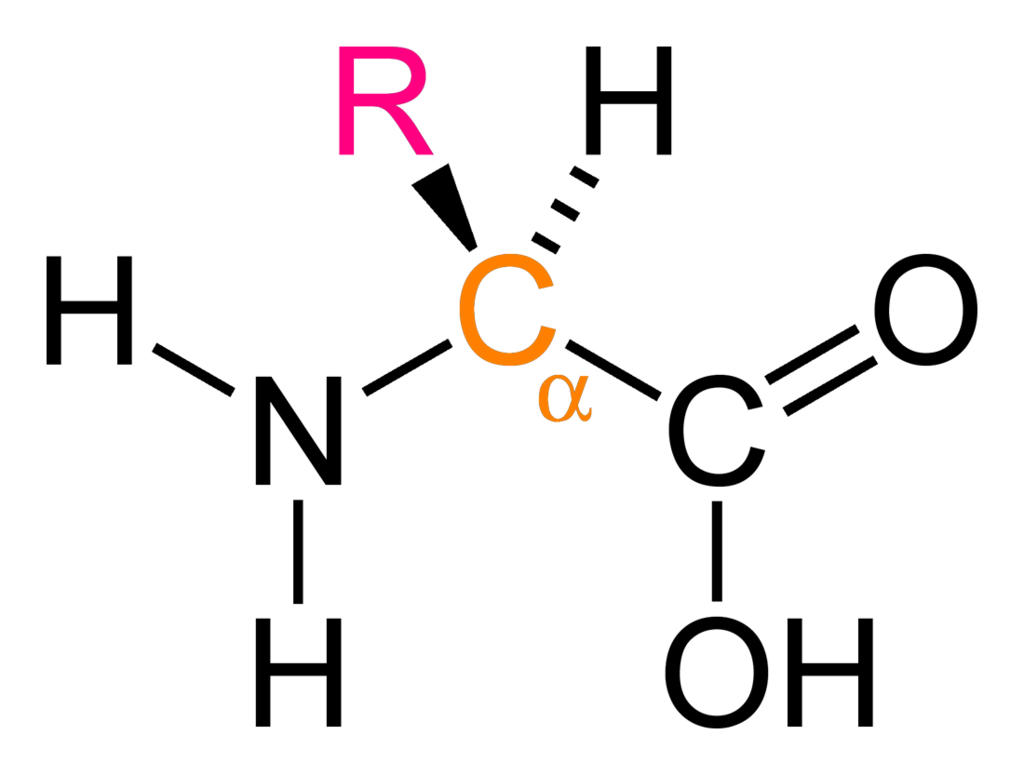
\includegraphics[height=4cm]{./figures/ch1/amino_acid_structure}}
			\caption{Structure chimique d'un acide aminé.}
			\label{fig:amino_acid_structure}
		\end{subfigure}
		~
		\begin{subfigure}{.6\textwidth}
			\centering
			{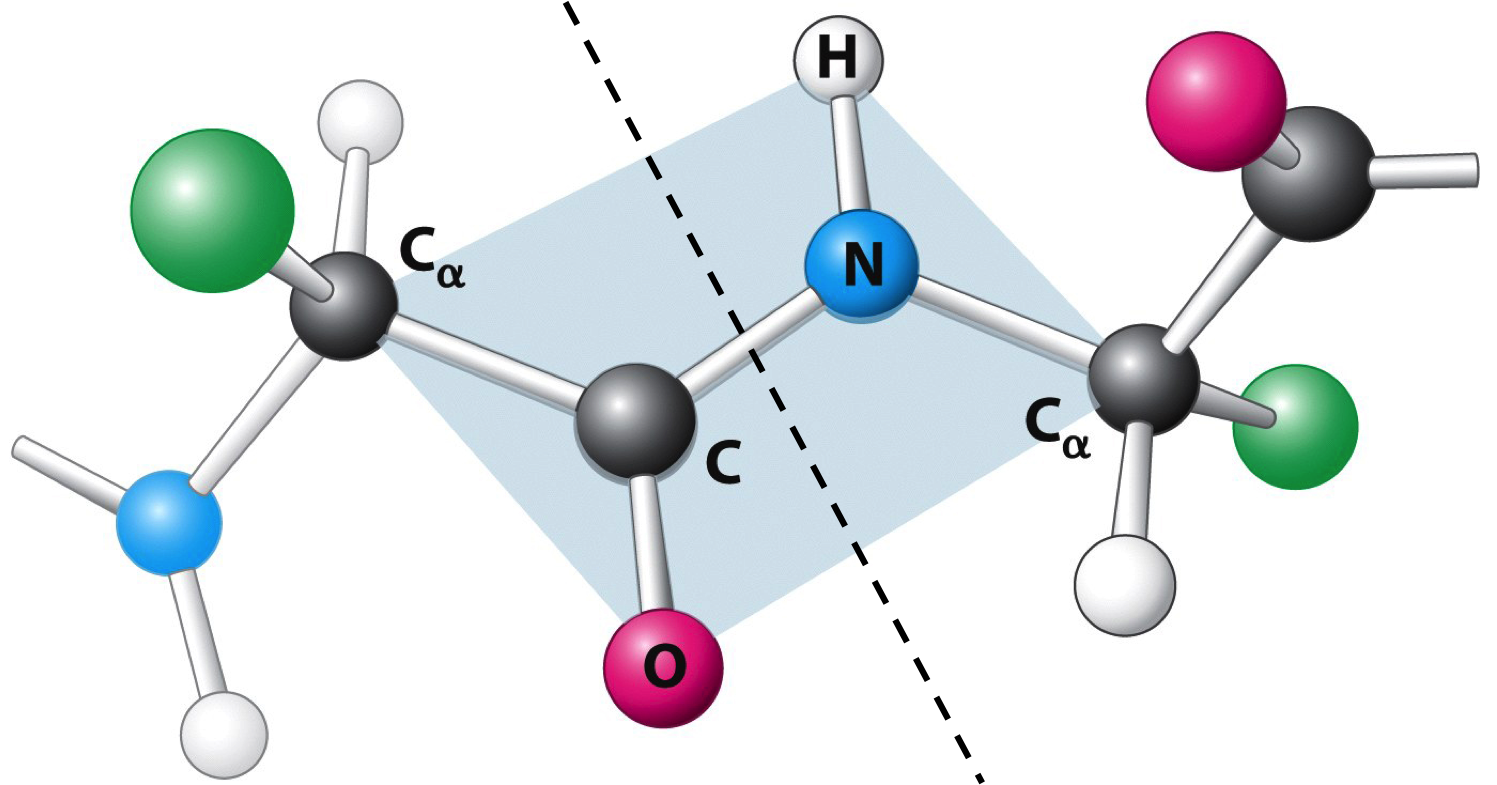
\includegraphics[height=4cm]{./figures/ch1/peptidic_bond.png}}
			\caption{Illustration d'une liaison peptidique entre deux acides aminés (à gauche et à droite de la ligne pointillée). Cette liaison est une liaison covalente entre l'azote (N) de l'acide aminé de droite et le carbone (C) de l'acide aminé de gauche.}
			\label{fig:peptide_bond}
		\end{subfigure}
		\caption[Acide aminé.]{Représentation schématique d'un acide aminé et d'une liaison petptidique. Crédit :~\cite{berg_biochemistry_2012}}
		\label{fig:aminoAcid}
	\end{figure}
	
	\begin{figure}[H]
		\centering
		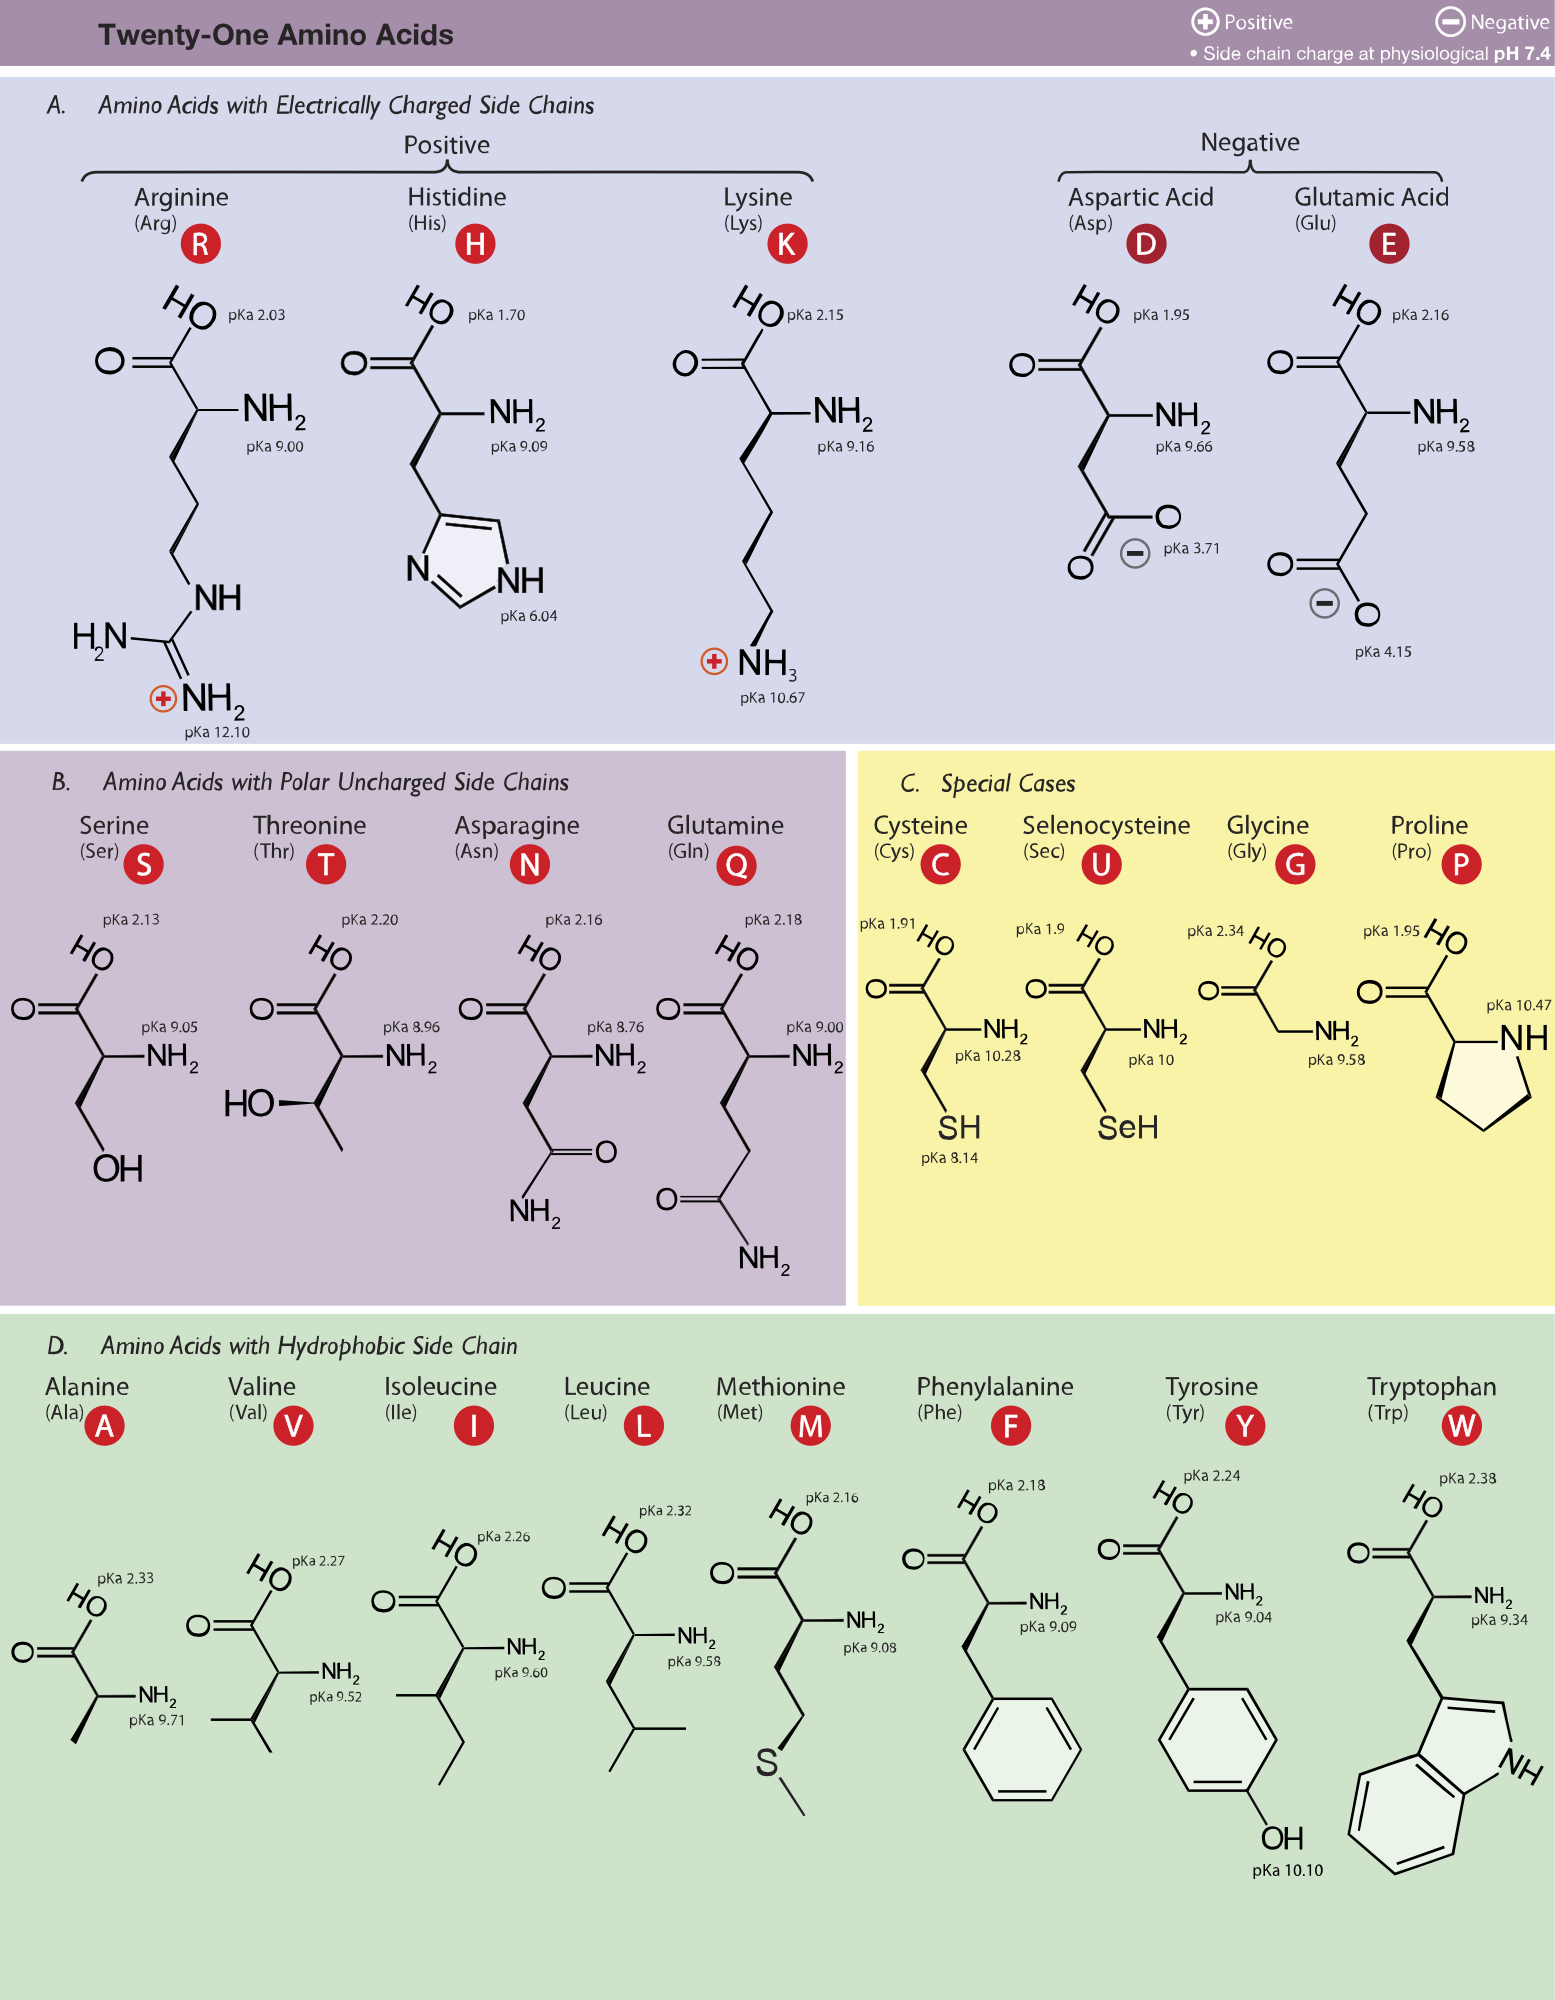
\includegraphics[width=\textwidth]{figures/ch1/aminoAcids}
		\caption[Ensemble des acides aminés.]{Les 21 acides aminés dits protéinogènes que l'on trouve chez les eukaryotes, c'est-à-dire ceux qui sont incorporés dans leurs protéines lors de la traduction de l'ARN messager par les ribosomes --- des complexes ribonucléoprotéiques dont la fonction est de synthétiser les protéines. Sur cette illustration, les acides aminés sont groupés en fonction des propriétés de leurs chaînes latérales, ici représentées \og au bas \fg{} des acides aminés. Crédit : \emph{Wikimedia}.}
		\label{fig:aminoAcids}
	\end{figure}
    
	\begin{figure}[H]
		\centering
		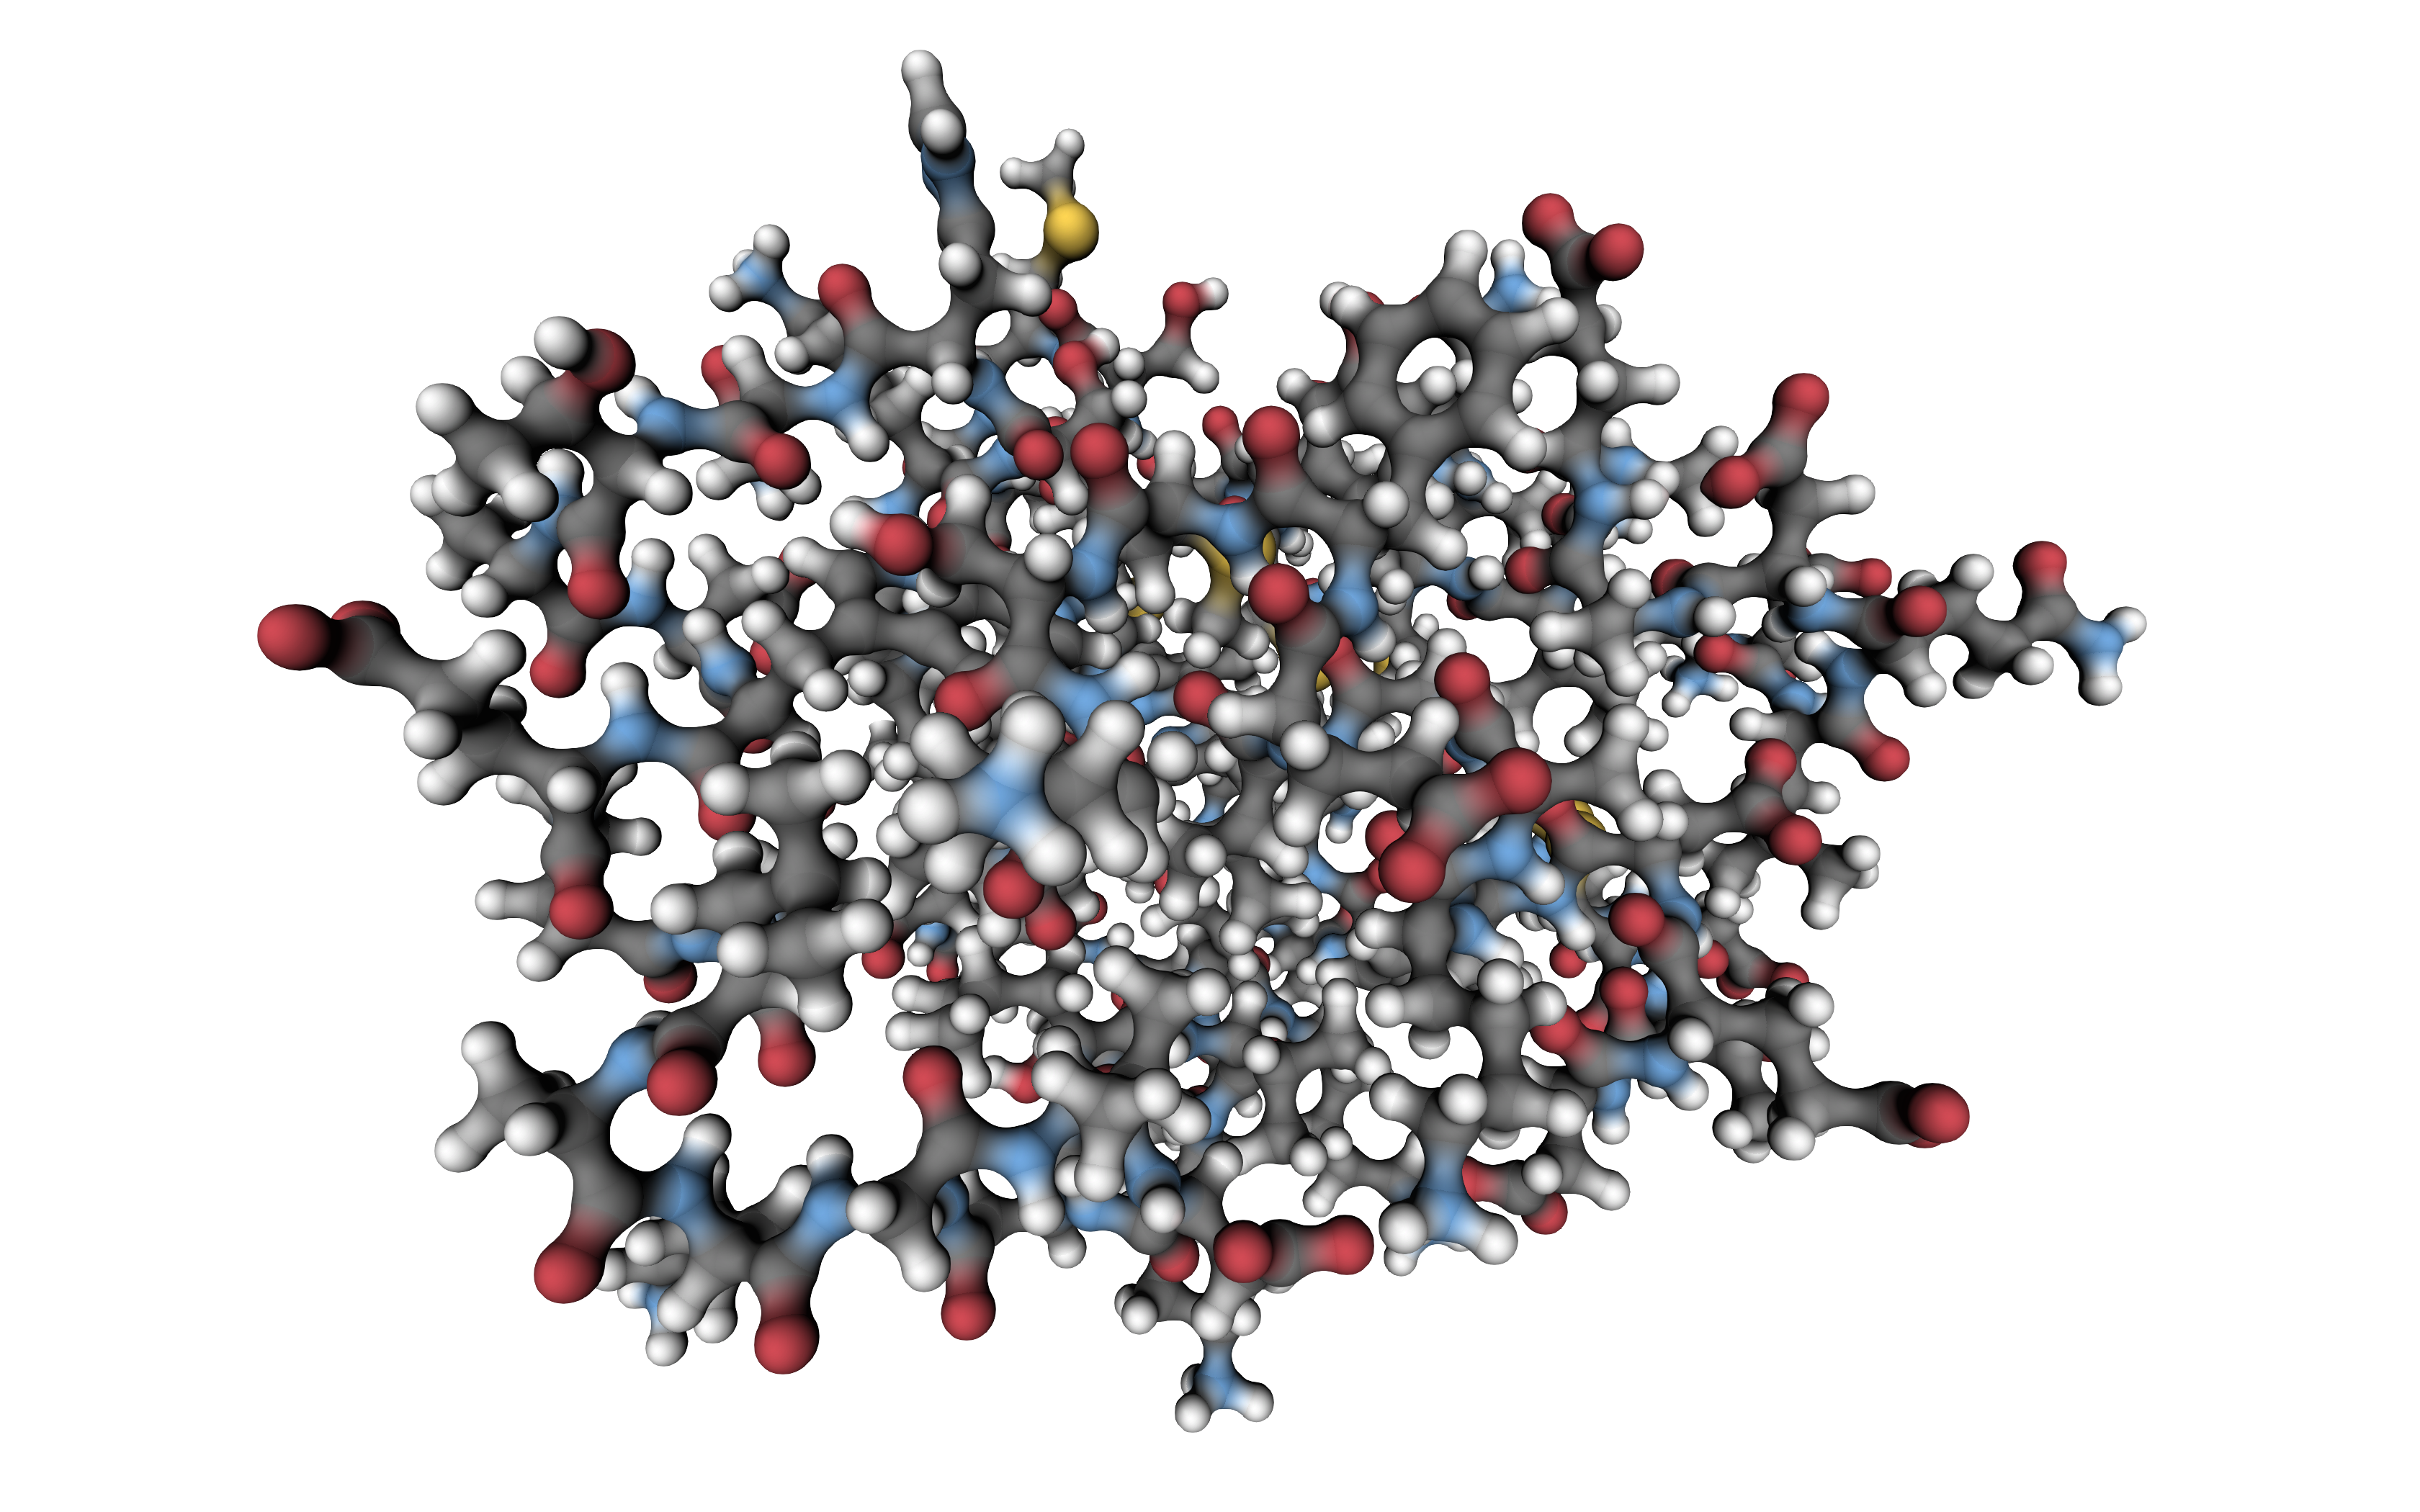
\includegraphics[width=\textwidth]{figures/ch1/1KX2}
		\caption{Illustration d'une protéine (\emph{1KX2}, un mono-hème ferrocytochrome~\cite{bartalesi2002solution}) produite avec le logiciel UnityMol~\cite{doutreligne2014unitymol}. Les atomes de carbone sont représentés en gris, ceux d'oxygène en rouge, d'hydrogène en blanc, et de soufre en jaune. Cette protéine est relativement petite, avec seulement 81 acides aminés (à comparer avec les quelque 30~000 de la titine, ou connectine) ; de plus, ce mode de représentation, dans lequel les atomes ont un rayon inférieur à leur rayon de van der Walls, couramment utilisé, minimise l'occultation ; néanmoins, on constate qu'une très grande partie de la molécule est occulée par les atomes situés au premier plan. De surcroît, il s'agit ici d'une représentation \emph{in vacuo}, c'est-à-dire sans le solvant dans lequel une protéine se trouve généralement à l'état naturel.}
		\label{fig:1KX2}
	\end{figure}
	
	\paragraph{Rôles.}
	Les protéines sont impliquées dans la plupart des processus biologiques et, de fait, leurs rôles sont extrêmement divers. On peut toutefois les diviser en deux grandes parties : les fonctions cellulaires et les fonctions biochimiques. Les premières définissent le rôle de la protéine dans la cellule ou l'organisme, et peuvent être découpées en cing groupes~\cite{lodish1995molecular} :
	\begin{enumerate}
		\item Les protéines des structures, qui permettent à la cellule de maintenir son intégrité physique et son organisation dans l'espace. C'est par exemple la fonction du collagène, la protéine la plus abondante chez les mammifères~\cite{di2002mapping}, illustrée par la figure~\ref{fig:collagen}.
		\item Les protéines de transport, qui acheminent les molécules nécessaires aux fonctions cellulaires au sein des cellules, mais aussi à travers les membranes nucélaires et plasmique, ou hors des cellules. Cela inclut notamment le transport de dioxygène par l'hémoglobine, de fer par la transferrine~\cite{crichton1987iron} (illustrée par la figure~\ref{fig:transferrin}) ou d'ions à travers les membranes cellulaires, par les canaux ioniques. 
		\item Les protéines régulatrices, qui inhibent ou stimulent l'activité d'autres protéines, ou la transcription de gènes, ce qui permet réguler divers processus biologiques. Un exemple de réseau de régulation formé par plusieurs protéines est représenté par la figure~\ref{fig:regulation}.
		\item Les protéines de signalisation, qui reçoivent les signaux extérieurs (en se liant aux molécules qui les transmettent ou en réagissant à leur contact) et assurent leur transmission vers la cellule, ou vers une autre zone de l'organisme. Les protéines de signalisation permettent notamment de réagir aux hormones ; lorsque celles-ci sont hydrophiles (et donc incapables de traverser la membrane cellulaire, composée de lipides) les protéines réceptrices sont transmembranaires, leur extrémité extérieure permet la fixation de l'hormone, tandis que l'extrémité intérieure transmet le signal. C'est notamment le cas des récepteurs de l'insuline~\cite{gammeltoft1984insulin}. Lorsque les hormones sont lipophiles et peuvent traverser la membrane, la protéine réagit à la fixation de l'hormone par un changement conformationnel qui lui permettra de transmettre le signal. C'est ainsi que fonctionnent les récepteurs d'œstrogène alpha, ou ER$\alpha$~\cite{dahlman2006international}, illustrés par la figure~\ref{fig:eralpha}.
		\item Les protéines motrices, qui permettent aux cellules ou aux organismes de se mouvoir. On peut citer par exemple la myosine, essentielle à l'activité musculaire des vertébrés~\cite{pollard1973acanthamoeba}, et illustrée par la figure~\ref{fig:myosin}.
	\end{enumerate}	

	\begin{figure}[H]
		\begin{subfigure}[t]{.4\textwidth}
			\centering
			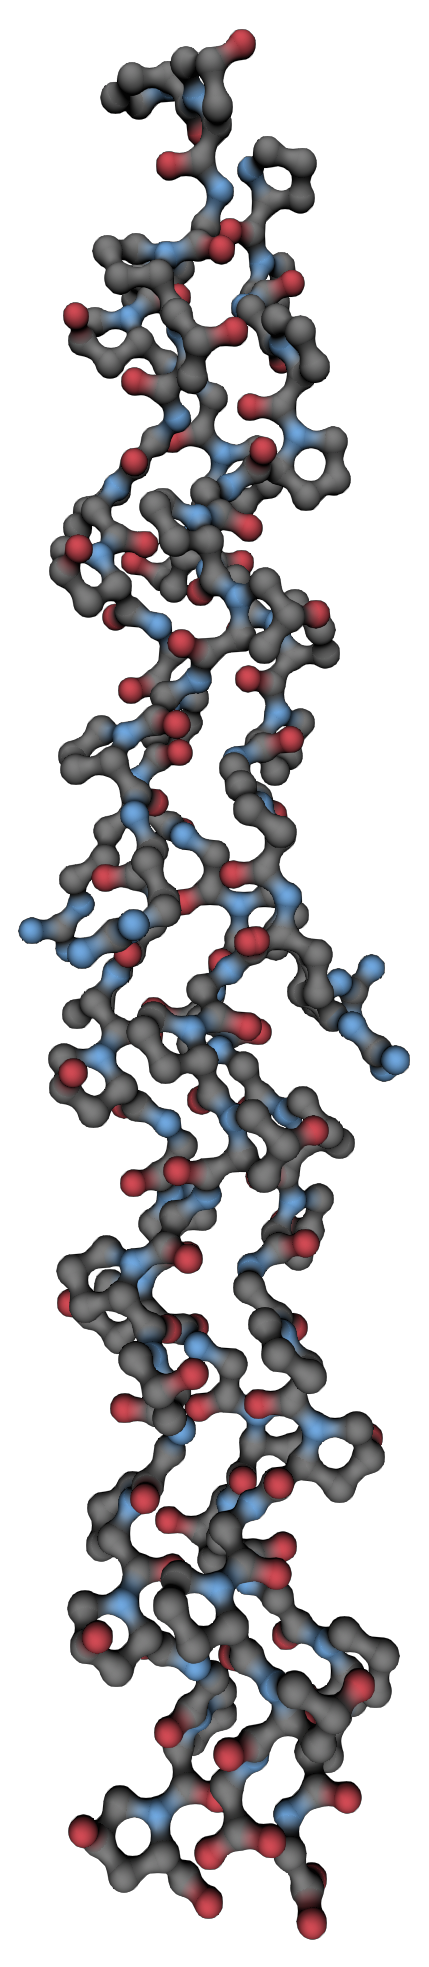
\includegraphics[height=7cm]{./figures/ch1/collagen}
			\caption[Collagène.]{Collagène : structure en triple-hélice d'arginines ; structure cristallographique~\cite{okuyama2014preferred}.}
			\label{fig:collagen}
		\end{subfigure}
		~
		\begin{subfigure}[t]{.6\textwidth}
			\centering
			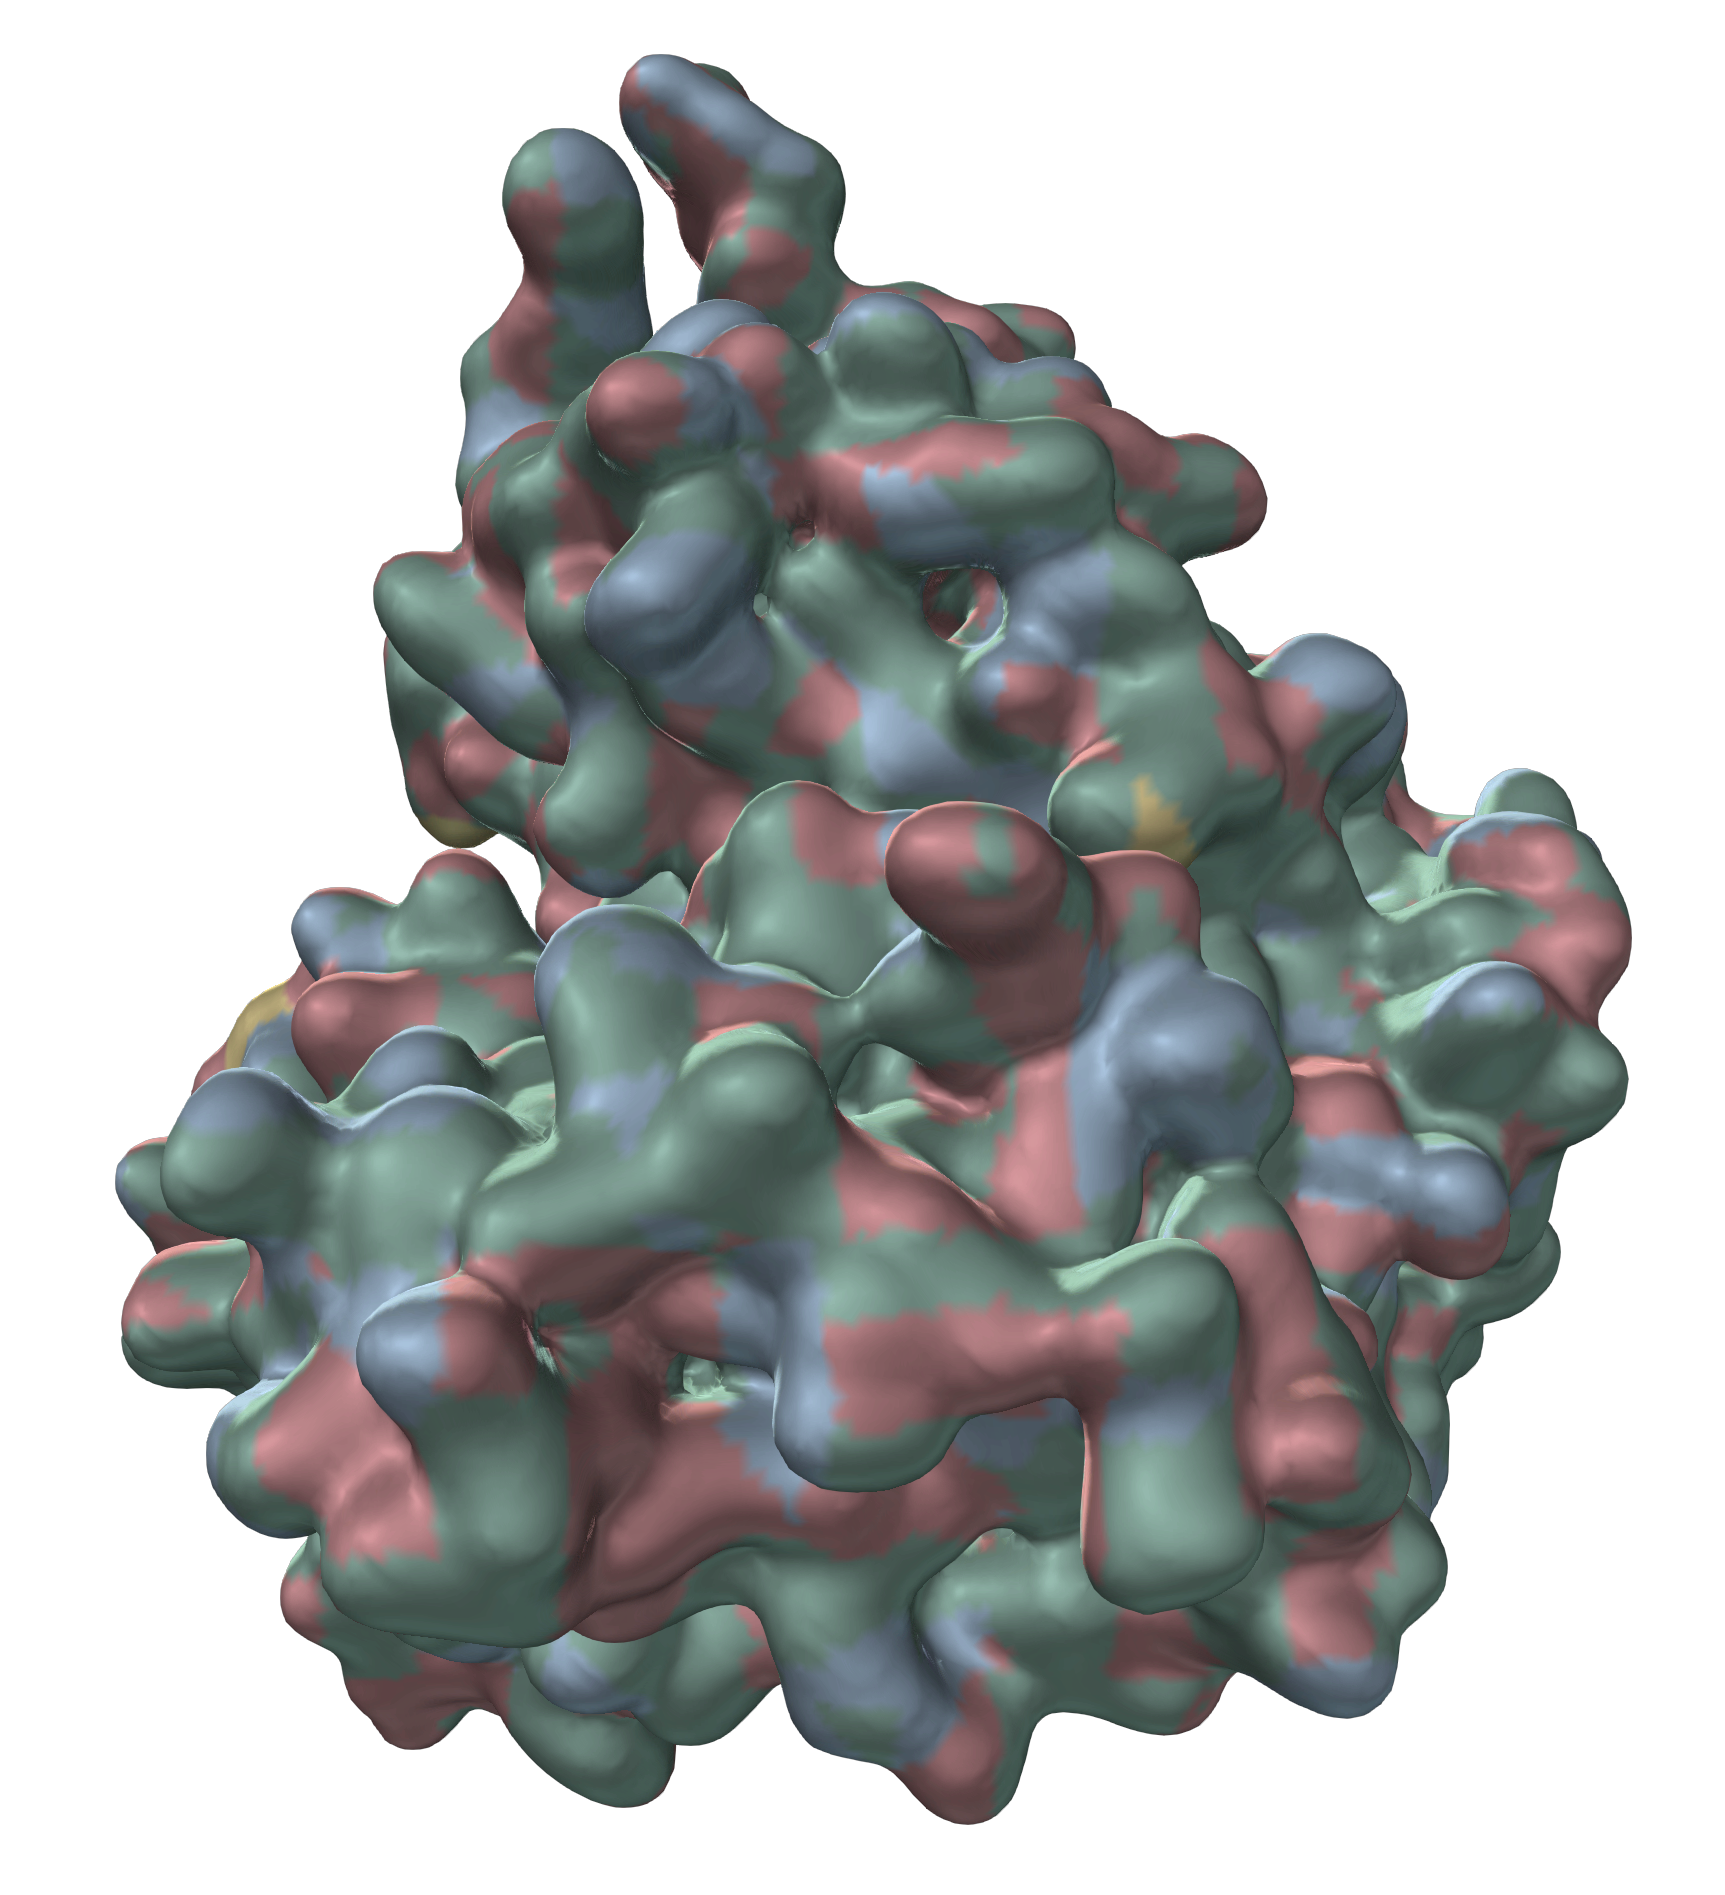
\includegraphics[height=7cm]{./figures/ch1/eralpha}
			\caption[Récepteur d'œstrogène alpha.]{Récepteur d'œstrogène alpha, représenté par une isosurface de densité colorée en fonction des atomes sous-jacents~\cite{nwachukwu2016systems}.}
			\label{fig:eralpha}
		\end{subfigure}
		\caption[Protéines de structure et de communication.]{Protéines de structure et de communication. Illustrations produites par \emph{UnityMol}.}
		\label{fig:prot_misc}
	\end{figure}
	
	\begin{figure}[H]
		\centering
		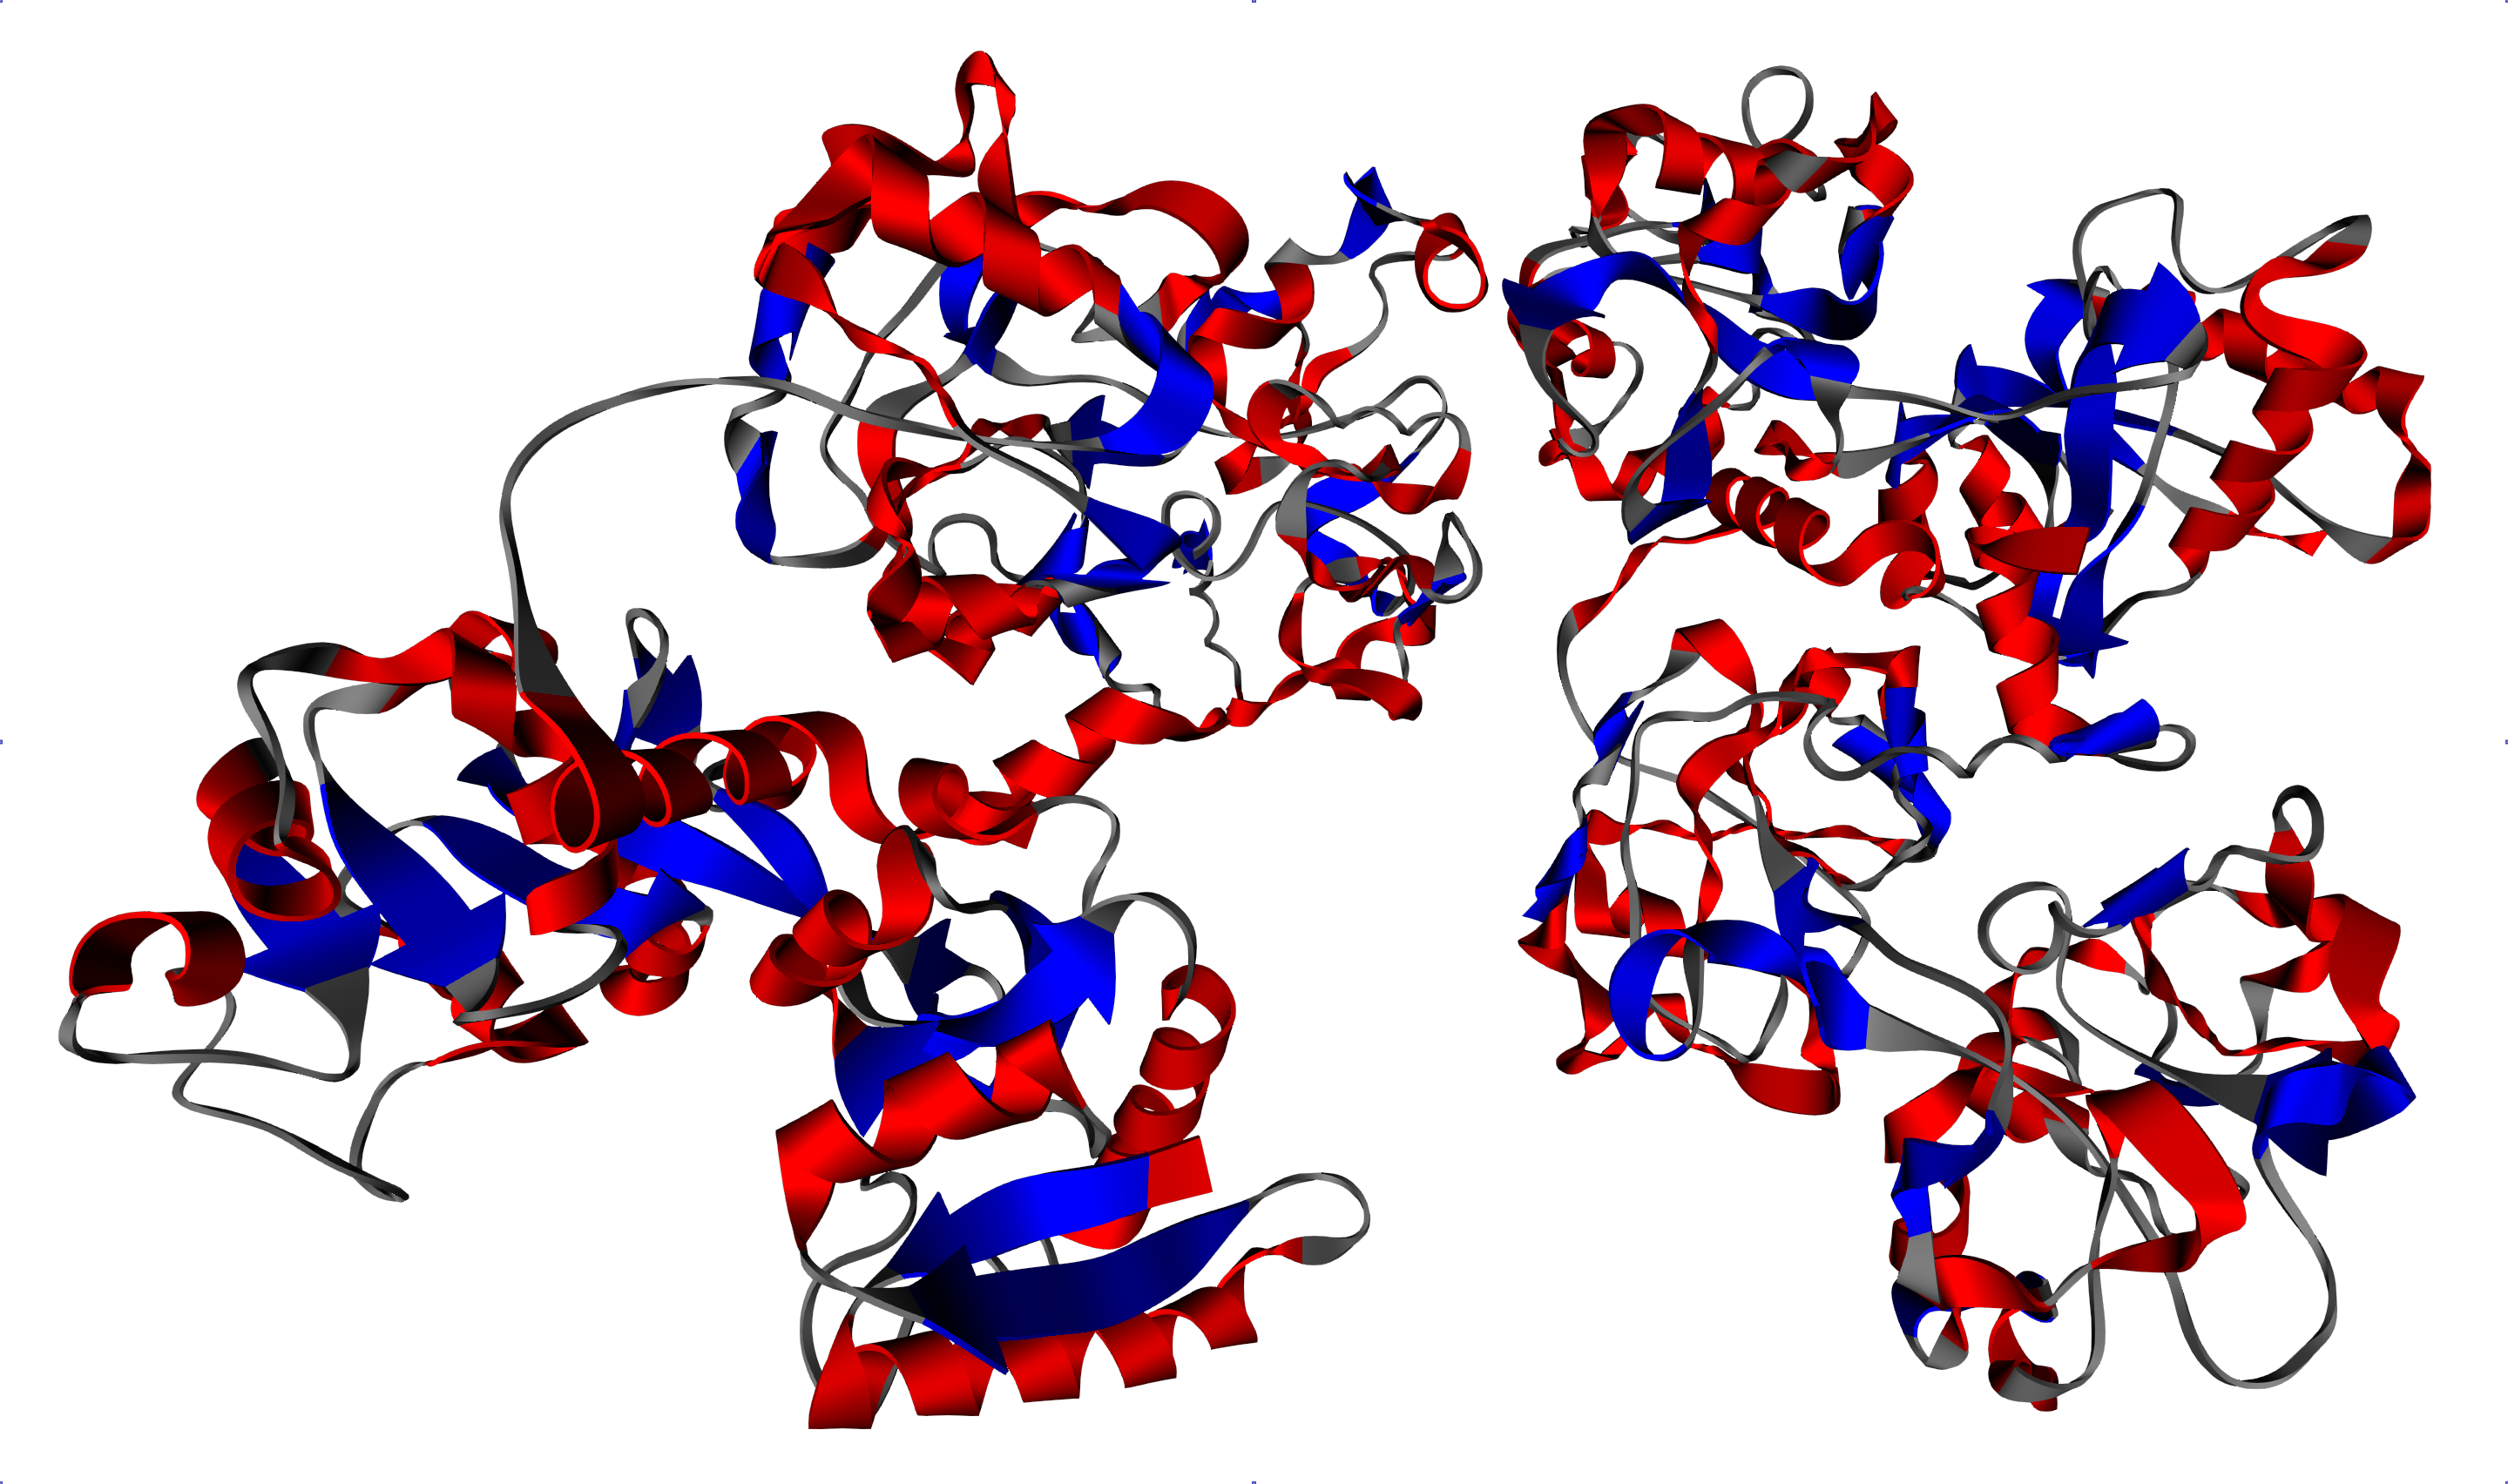
\includegraphics[width=\textwidth]{figures/ch1/transferrin}
		\caption[Transferrine.]{Illustration d'une protéine de transport : la transferrine humaine, ici liée à de l'ytterbium, et représentée par ses structures secondaires (hélices alpha en rouge et feuillets bêta en bleu). Illustration produite par \emph{UnityMol} à partir d'une structure de la \emph{Protein Data Bank}~\cite{wang2015anion}.}
		\label{fig:transferrin}
	\end{figure}
	
	\begin{figure}[H]
		\centering
		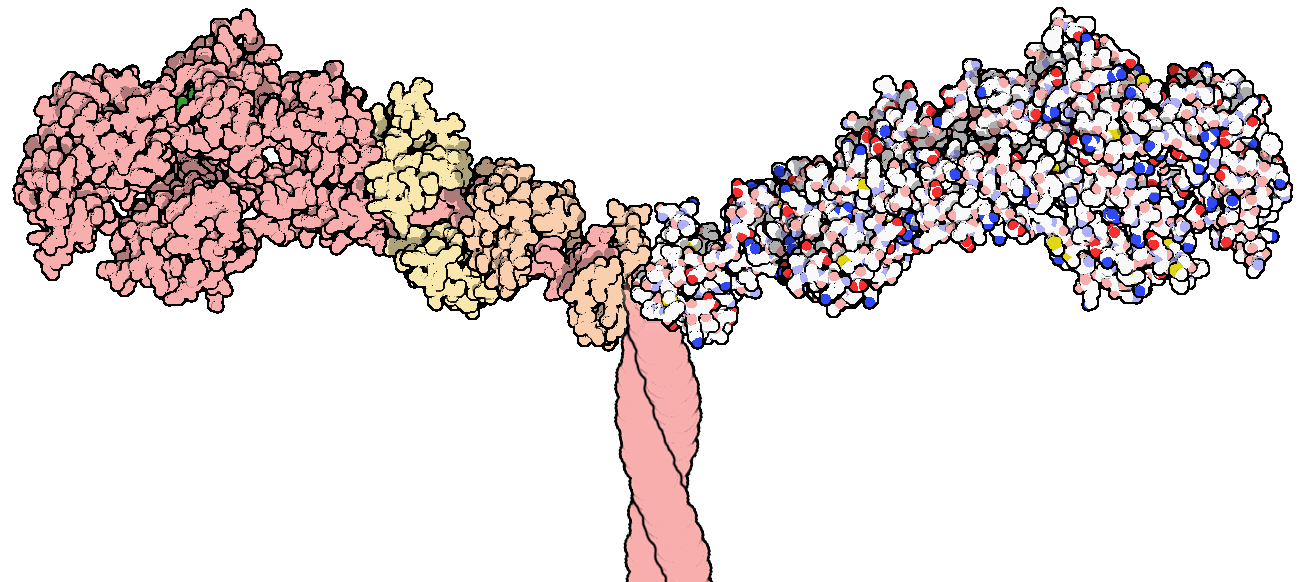
\includegraphics[width=\textwidth]{figures/ch1/myosin}
		\caption[Myosine.]{Illustration d'une portion de myosine, une protéine essentielle à l'activité contractile des vertébrés, notamment dans les cellules musculaires. Illustration de David Goodsell, à partir d'une structure de la \emph{Protein Data Bank}~\cite{houdusse1999atomic}.}
		\label{fig:myosin}
	\end{figure}
	
	\begin{figure}[H]
		\centering
		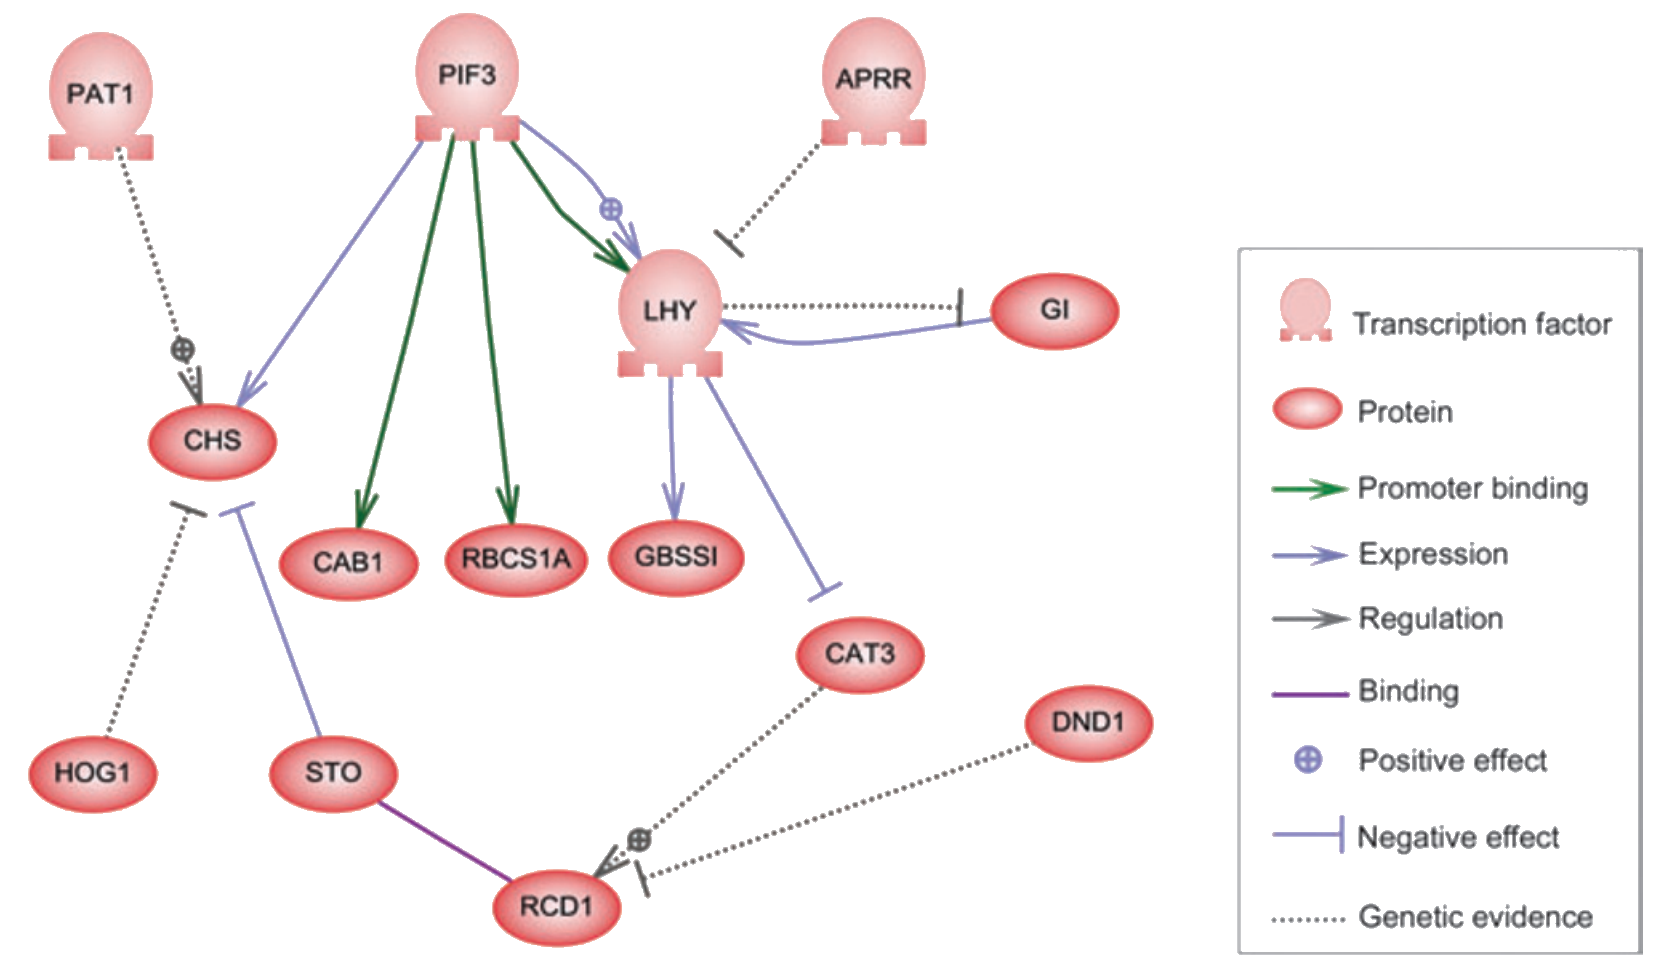
\includegraphics[width=\textwidth]{figures/ch1/regulation}
		\caption[Réseau de régulation.]{Schéma représentant un réseau de régulation génétique (chez une espèce de riz hybride). Les ellipses roses-rouges représentent des protéines, et les disques roses représentent des facteurs de transcription\footnotemark. Les interactions sont multiples, et peuvent prendre la forme d'une liaison, d'une stimulation, d'une inhibition\ldots{} Les protéines sont impliquées à tous les niveaux du processus. Crédit :~\cite{song2010comparative}.}
		\label{fig:regulation}
	\end{figure}
	
	\footnotetext{Un facteur de transcription est une protéine qui contrôle le taux de transcription d'une portion d'ADN en ARN messager~\cite{latchman1997transcription}.}
	
	
	\subsection{Modes de représentation}
	Un atome n'est pas un objet au sens où on l'entend communément, dans un contexte macroscopique. S'il est courant de représenter un atome par une sphère, il n'a pas de rayon, de \og coquille \fg{} et ce n'est qu'une représentation schématique de la réalité, utilisée pour communiquer une information. Autour du noyau de l'atome se trouve un nuage électronique où les électrons occupent de manière probabiliste certaines régions de l'espace. Pour représenter ce nuage électronique, on peut procéder comme sur la figure~\ref{fig:helium}.
	
	\begin{figure}[H]
		\centering
		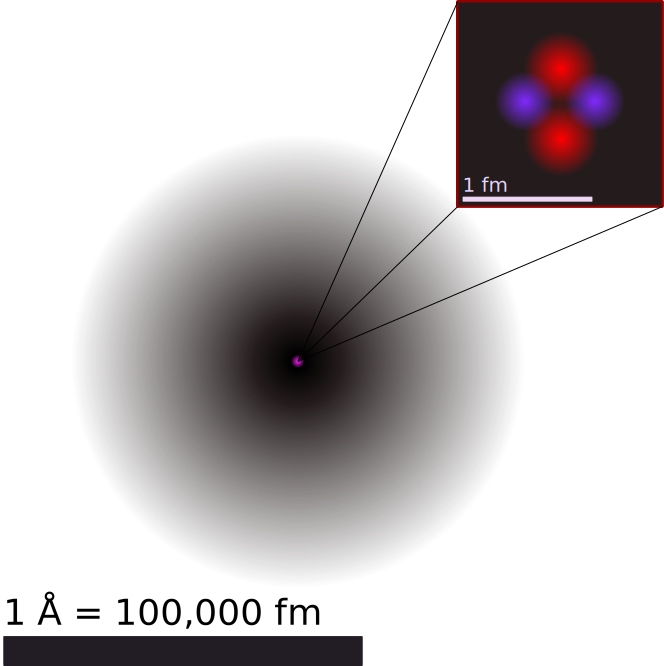
\includegraphics[width=\textwidth]{figures/ch1/helium}
		\caption{Illustration d'un atome d'hélium, représentant le noyau en rose et la distribution du nuage électronique en nuances de gris. Le noyau (en haut à droite) de l'hélium-4 est représenté de façon très schématisée. La barre noire en bas à gauche indique l'échelle, et mesure un \aa{}ngström, soit $0,1$ nanomètre. Crédit : \emph{Wikimedia}.}
		\label{fig:helium}
	\end{figure}
	
	\paragraph{Points.} Le mode de visualisation le plus simple consiste à représenter chaque atome (et uniquement les atomes) par un point tout juste assez gros pour être visible. Les liaisons covalentes ne sont pas représentées. Selon la façon dont elle est mise en œuvre, cette technique de visualisation peut être très performante, et donc garantir un affichage fluide même avec de très nombreux atomes. Elle a de plus l'avantage de minimiser l'occultation des atomes les uns par les autres, du fait de leur petite taille. Cependant, elle communique peu d'informations sur la molécule. En particulier, les liaisons covalentes étant absentes, sa structure même fait défaut. De plus, l'utilisateur peut difficilement se faire une idée de l'espace qu'occupe réellement cette molécule dans son milieu, car chaque atome n'est représenté que schématiquement, par un point bien plus petit que ce que l'on observe sur la figure~\ref{fig:helium}, par exemple.
		
	Enfin, elle rend difficile l'appréciation de la position d'un atome par rapport à ceux qui, dans le plan de l'écran (projeté) se trouvent à proximité, car seule la taille du point permet d'estimer sa distance par rapport à l'observateur. Or, comme les atomes ne font pas tous précisément la même taille, cette appréciation ne peut être que très approximative, même dans le cas où la couleur du point indiquerait la nature de l'atome représenté à une utilisateur connaissant la taille de l'atome en question. La figure~\ref{fig:4awn_points} présente un exemple de cette technique de visualisation. L'on comprend que, si la représentation en points présente certains avantages par rapport à une tâche de sélection, elle est par ailleurs trop limitée pour être apprécié des physico-chimistes ou biologistes souhaitant intéragir avec des simulations moléculaires.
	    
	\paragraph{Bâtons ou réglisse.} Un autre mode de visualisation assez simple consiste à représenter uniquement les liaisons covalentes par des traits ou bâtons, juste assez épais pour être clairement visibles, ou par de petits cyclindes ou parallélépipèdes rectangles. Cette représentation est aussi parfois appelée \og réglisse \fg{} ou \emph{licorice}, en anglais. Si les atomes eux-mêmes ne sont pas explicitement représentés, ils se trouvent à l'intersection des liaisons covalentes où à leurs extrémités, et la coloration de ces liaisons indique la nature des atomes qu'elles relient.
		
	Dans une moindre mesure, cette technique de visualisation reprend les avantages de celle en points, puisque le niveau d'occultation, s'il est plus élevé, demeure assez faible. Le coût en ressources de calcul n'est pas nécessairement plus élevé que pour la représentation en points, ce qui permet également d'obtenir de très bonnes performances, même losque l'on affiche des systèmes très complexes. Un exemple est fourni dans la figure~\ref{fig:4awn_licorice}.
		
	La visualisation en réglisse, puisqu'elle affiche les liaisons covalentes, représente la structure de la molécule, et la représente même particulièrement clairement. Ses propriétés physico-chimiques peuvent donc être déduites de la représentation, du moins par un utilisateur expert. Par ailleurs, la distance d'un atome par rapport à la caméra est un peu plus facile à apprécier, car l'utilisateur dispose de plus de repères visuels (bien que ceux-ci puissent également occulter totalement l'atome, rendant sa localisation encore plus difficile). Elle partage cependant un inconvénient avec la visualisation en points, puisqu'elle communique à peu près aussi mal l'espace occupé par la protéine, en la réduisant visuellement à son \og squelette \fg{}. Selon les cas, cet inconvénient peut être plus ou moins gênant.
		
	Cette représentation dispose de suffisamment d'avantages pour être utilisée assez fréquemment. Par conséquent, elle constitue un cas d'application important pour les contributions présentées plus loin.
		
	\paragraph{Boules et bâtons, ou CPK.} Une technique de visualisation très courante est appelée \og en boules et bâtons \fg{} (ou \emph{ball-and-stick}, en anglais). Elle est parfois appelée CPK, un peu par abus de langage, en référence aux modèles physiques créés par les chimistes Robert \textbf{C}orey, Linus \textbf{P}auling, et améliorés par Walter \textbf{K}oltun~\cite{corey1953molecular, koltun1965space} ainsi qu'à la convention de couleurs CPK qui est souvent utilisée avec cette représentation. Cette convention est essentiellement caractérisée par l'utilisation du noir pour le carbone, du blanc pour l'hydrogène, du rouge pour l'oxygène, du bleu pour l'azote, du jaune pour le soufre, du violet pour le phosphore, de nuances de vert pour les halogènes (fluore, chlore, brome, iode) et du gris argent pour les métaux.
		
	Ce mode de visualisation, que nous désignerons ci-après par l'appellation \emph{CPK}, représente chaque atome par une sphère, et chaque liaison covalente par un bâton, comme dans la représentation par bâtons. Il s'agit comme dans cette dernière de bien représenter la structure de la molécule, mais en insistant plus sur les atomes. Traditionnellement, ceux-ci sont toutefois représentés par des sphères nettement plus petites que le rayon de van der Waals des atomes (voir le mode suivant).
		
	Outre le fait qu'elle correspond aux modèles physiques CPK, comme celui de la figure~\ref{fig:aspirin}, cette représentation permet de bien visualiser la structure de la molécule et la nature de ses atomes. Naturellement, l'utilisation de sphères implique un degré d'occultation accru par rapport à la représentation en bâtons, mais elle permet aussi d'avoir une meilleure appréciation du volume occupé par la molécule.
		
	Sur ce dernier point, la représentation en boules et bâtons a néanmoins ses limites, puisqu'elle occupe un volume réduit par rapport à certaines références pertinentes d'un point de vue physico-chimique, liées au rayon de van der Waals ou à la densité moléculaire, comme détaillé dans les descriptions des représentations suivantes.
		
	\paragraph{Sphères de van der Waals.} La représentation en sphères de van der Waals repose sur la notion de rayon de van der Waals. Celle-ci découle elle même de la force de van der Waals~\cite{dzyaloshinskii1961general}. Il s'agit en fait de l'effet combiné de plusieurs forces :
	
	\begin{itemize}
	    \item Les interactions électrostatiques (attractives et répulsives) entre des multipôles permanents, parfois appelées Forces de Keesom~\cite{keesom1915second} ;
		\item L'induction (ou polarisation), c'est-à-dire l'interaction électrostatique attractive entre un multipôle permanent et un multipôle induit, également appelée force de Debye~\cite{debye1913reprinted, debye1929polar} ;
	    \item La dispersion, c'est-à-dire l'interaction électrostatique attractive entre deux multipôles induits, aussi désignée force de London~\cite{eisenschitz1930verhaltnis, london1930theorie, london1937general} ;
		\item La répulsion de Pauli, qui découle du principe d'exclusion de Pauli~\cite{pauli1925zusammenhang}, selon lequel plusieurs électrons (et autres fermions) ne peuvent pas se trouver simultanément dans le même état quantique. En effet, attendu que les électrons de deux atomes ne peuvent pas occuper le même espace simultanément, des atomes dont les nuages électroniques se croisent sont soumis à une force répulsive.
	\end{itemize}
	
	Les logiciels de simulation utilisent fréquemment le potentiel de Lennard-Jones~\cite{lennard1924determination} pour modéliser les forces de van der Waals. Celui-ci peut s'exprimer par l'équation~\ref{eq:lennard}, où $r$ est la distance entre les centres des deux atomes concernés, et $d$ représente la distance pour laquelle le potentiel de Lennard-Jones est nul ; $E_{0}$ est la valeur minimale du potentiel, soit le \og fond \fg{} du puits de potentiel. Comme on l'observe aisément sur la figure~\ref{fig:lennard}, le potentiel admet un minimum, dont on peut déduire un rayon de van der Waals. Ce rayon peut être celui d'une sphère représentant l'atome en question. La figure~\ref{fig:vdwradius} en fournit une illustration.
		
	\begin{figure}[H]
		\centering
		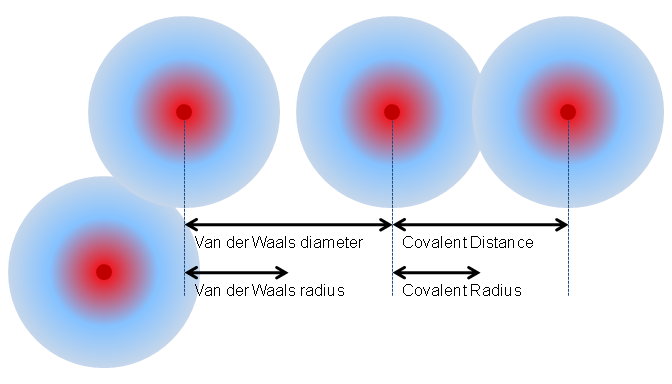
\includegraphics[width=\textwidth]{figures/ch1/vdwradius}
		\caption{Représentation du rayon de van der Waals, par opposition au rayon de covalence, plus petit. En effet, celui-ci est défini par la longueur d'une liaison covalente, qui implique le partage d'électrons entre une paire d'atomes. Le rayon de van der Waals, lui, correspond à une paire d'atomes non liés. C'est pour cette raison qu'en représentation de van der Waals, les atomes liés semblent imbriqués les uns dans les autres. Crédit : Chemistry -- LibreTexts\protect\footnotemark.}
		\label{fig:vdwradius}
	\end{figure}
	
\footnotetext{\url{http://chem.libretexts.org/Core/Physical_and_Theoretical_Chemistry/Chemical_Bonding/General_Principles_of_Chemical_Bonding/Covalent_Bond_Distance,_Radius_and_van_der_Waals_Radius}}
    
	C'est le principe de la représentation en sphères de van der Waals, illustrée par la figure~\ref{fig:4awn_VdW}. Ce mode de visualisation a plusieurs avantages. Premièrement, il correspond à une réalité physique, celle des forces de van der Waals. Deuxièmement, il permet d'apprécier le volume occupé par la molécule. Troisièmement, les atomes étant représentés par de grosses sphères, ils sont mieux visibles pour un niveau de zoom donné. De fait, il est plus aisé d'envisager les interactions possibles entre cette molécule et une autre, puisque l'on perçoit mieux les volumes des cavités dans lesquelles d'éventuels ligands pourraient venir se loger, et la bonne visualisation des atomes à la surface peut aider à évaluer la probabilité d'un arrimage avec ledit ligand.
		
	Cependant, les liaisons covalentes sont totalement occultées, et il est seulement possible de les \og deviner \fg{} à partir de l'emplacement des atomes et grâce aux lois de la chimie. La structure de la molécule est donc beaucoup moins claire qu'en représentation CPK, par exemple. De plus, les atomes sont si gros qu'ils occultent totalement ceux qui sont derrière eux. De fait, l'intérieur de la molécule devient totalement invisible. Si sa surface est mieux représentée, sa structure interne est entièrement occultée. C'est plus gênant encore lorsque les atomes d'hydrogène sont affichés, ce qui n'est pas le cas sur la figure~\ref{fig:4awn_VdW} --- il est courant de les omettre, par souci de clarté. Selon la mise en \oe{}uvre logicielle de cette représentation, elle peut être coûteuse en ressources de calcul, même si des solutions efficaces existent. En mouvement, la grande taille des atomes a l'avantage de diminuer leur mouvement relatif, c'est-à-dire leur mouvement par rapport à eux-mêmes.
		
	Les sphères de van der Waals ne sont pas une mauvaise option pour visualiser (ou interagir avec) une simulation de dynamique moléculaire, à condition que l'objet d'intérêt principal soit superficiel, et donc bien visible. La grande taille des cibles peut être un avantage, même s'il y a un certain degré d'interpénétration entre elles. Cette représentation constitue donc un cas d'application notable pour une technique de sélection de cibles mobiles.
		
	\begin{equation}
		\label{eq:lennard}
		E_{p}\left(r\right) = 4E_{0} \left( \left(\frac{d}{r}\right)^{12} - \left(\frac{d}{r}\right)^{6} \right)
	\end{equation}
		
	\begin{figure}[H]
		\centering
		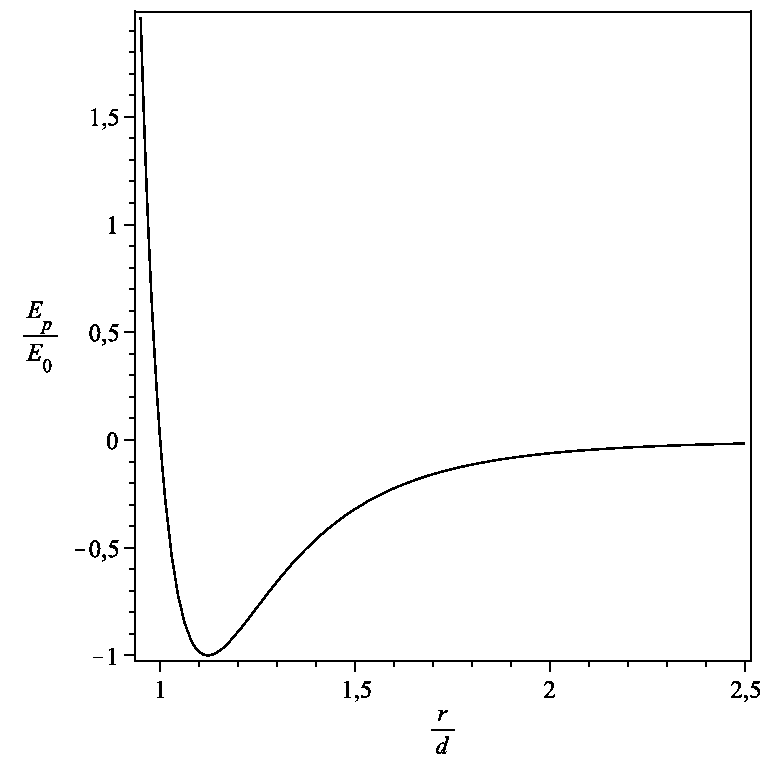
\includegraphics[width=\textwidth]{figures/ch1/lennard-jones}
		\caption[Représentation graphique du potentiel de Lennard-Jones.]{Représentation graphique du potentiel de Lennard-Jones, en fonction du rapport $r/d$ entre la distance interatomique réelle et celle pour laquelle le potentiel s'annule. Le potentiel admet un minimum en $r/d = 2^{1/6}$, soit environ $1,12246$. Crédit : \emph{Wikimedia}.}
		\label{fig:lennard}
	\end{figure}
		
	\paragraph{\emph{Hyperballs}.} La technique de visualisation de molécules appelée \emph{Hyperballs}~\cite{chavent2011gpu} se base sur une représentation analytique des atomes et des liaisons covalentes. Leurs surfaces sont décrites par des équations, des rayons sont lancés vers les atomes, et il s'agit ensuite de résoudre des équations d'intersection entre les rayons et les surfaces.
		
	Les \emph{Hyperballs} présentent de nombreux avantages. Sur le plan purement technique, leur mode de représentation analytique permet, au contraire des maillages de points (\emph{meshes}, en anglais) d'éviter d'avoir à gérer un très grand nombre de points et de triangles. De plus, quel que soit le niveau de zoom, les surfaces des sphères et des liaisons covalentes (représentées par des hyperboloïdes) demeurent parfaitement lisses. Comme l'illustre la figure~\ref{fig:spheremeshes}, avec des maillages, il est nécessaire d'avoir un grand nombre de triangles pour maintenir l'illusion de la rotondité du modèle lorsqu'il est observé de près.
		
	La figure~\ref{fig:hyperballs} illustre la représentation analytique des \emph{Hyperballs}, et sa légende détaille la façon dont on peut les utiliser pour \og imiter \fg{} les modes de représentation sus-cités. En réalité, les illustrations fournies jusqu'ici pour la représentation en points, en bâtons, en boules et bâtons, et en sphères de van der Waals ont toutes été produites avec des \emph{Hyperballs}, simplement en jouant sur leurs paramètres. Cette grande flexibilité, combinée aux performances de premier ordre offertes par cette technique (voir~\cite{chavent2011gpu}) rend cette technique particulièrement avantageuse.
		
	Au-delà de sa flexibilité, cependant, elle a l'avantage de permettre une représentation originale, avec des liaisons représentées par des hyperboloïdes. En jouant sur la courbure de ces hyperboloïdes, on peut communiquer des informations sur la nature de la liaison, par exemple sur la quantité d'énergie nécessaire à sa rupture. Si cette quantité est faible, on peut représenter la liaison par une hyperboloïde très \og creusée \fg{}, donnant l'impression d'être sur le point de rompre.
		
	Enfin, les \emph{Hyperballs}, utilisées de la façon la plus \og classique \fg{} ou \og canonique \fg{} présentent des hyperboloïdes partiellement creusées, comme sur la figure~\ref{fig:4awn_HB}. Cette représentation est souvent appréciée pour ses qualités esthétiques, certes subjectives. D'un point de vue plus objectif, la représentation en \emph{Hyperballs} canoniques présentent à peu près les mêmes caractéristiques que la représentation en boules et bâtons. Les dimensions sont proches, même si les formes diffèrent. Les liaisons sont un peu plus épaisses près des atomes, et comparables, voire un peu plus fines au milieu. De fait, la perception de la structure de la molécule et de ses propriétés, ainsi que le niveau d'occultation visuelle, sont assez comparables. Par conséquent, la représentation en \emph{Hyperballs} canoniques est un cas d'application aussi pertinent pour la sélection de cibles mobiles que la représentation CPK, voire plus, car les bonnes performances des \emph{Hyperballs} permettent de gérer de très gros systèmes plus facilement.
		
	\begin{figure}[H]
    	\centering
    	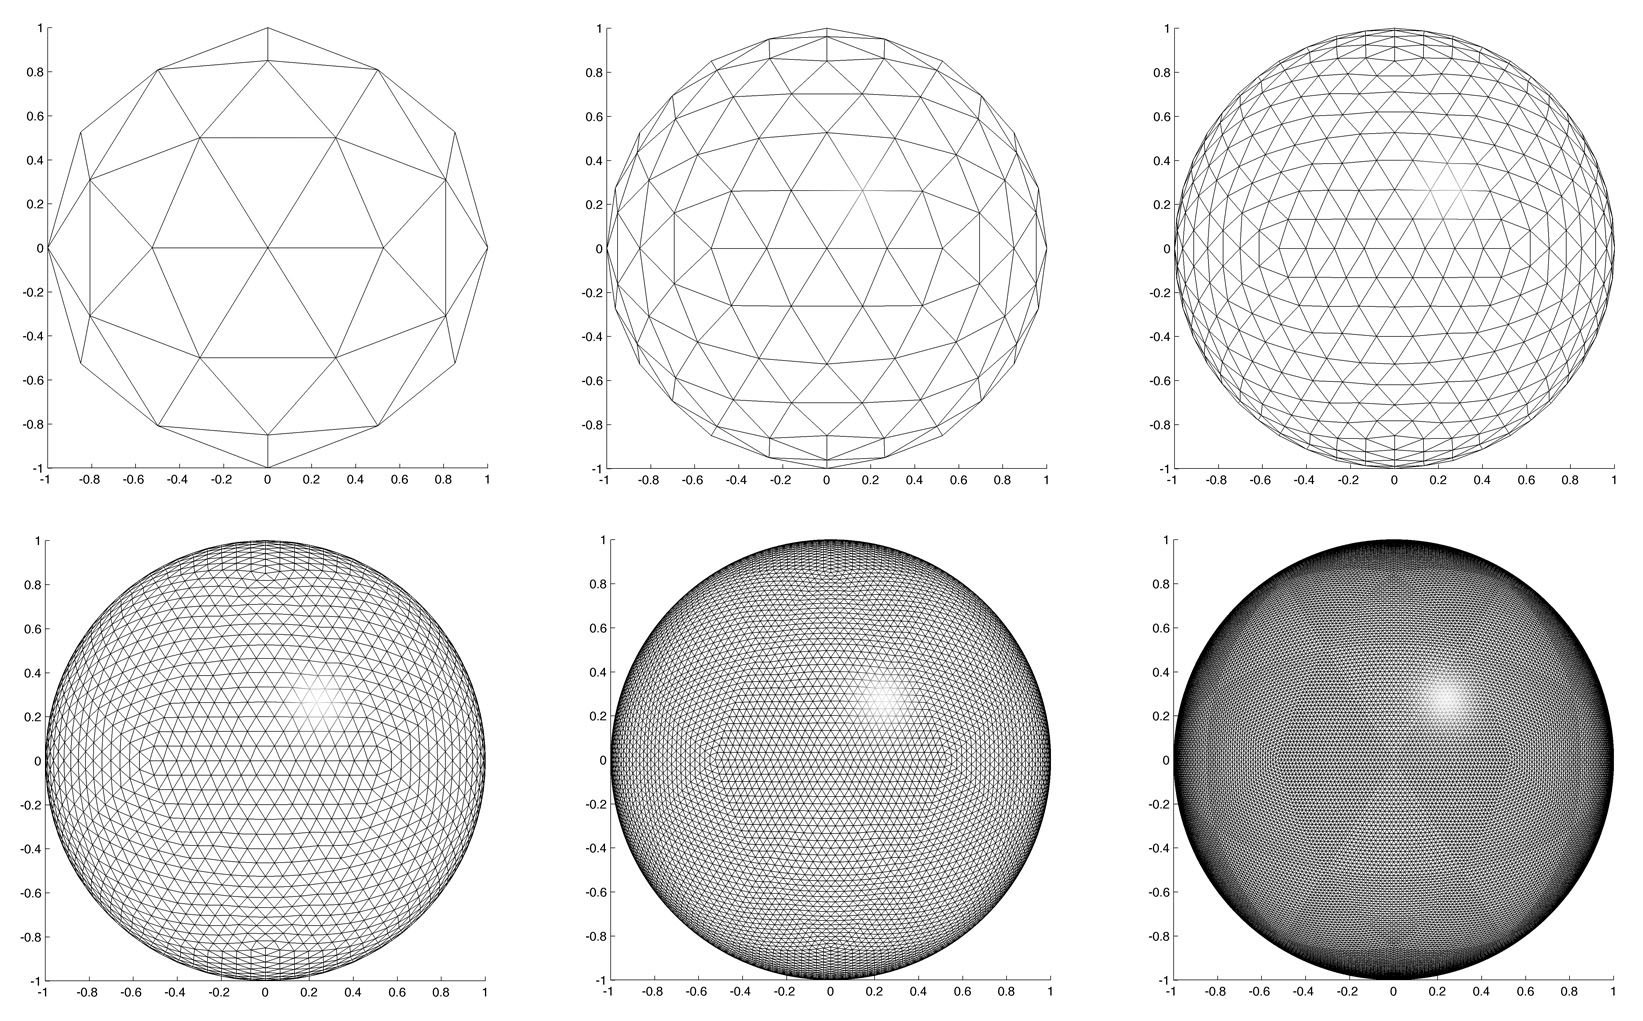
\includegraphics[width=\textwidth]{figures/ch1/spheremeshes}
    	\caption{Représentations d'une sphère par maillages de triangles, plus ou moins fins. Si un maillage grossier est économe en triangles (donc en ressources de calcul et en mémoire) il n'apparaît comme sphérique que de loin ; inversement, les maillages plus fins fournissent une illusion de rotondité convaincante, mais à un coût prohibitif. Du reste, un niveau de zoom très élevé peut briser cette illusion, même sur un maillage très fin. Crédit :~\cite{seo2010heat}.}
    	\label{fig:spheremeshes}
	\end{figure}
		
	\begin{figure}[H]
    	\centering
    	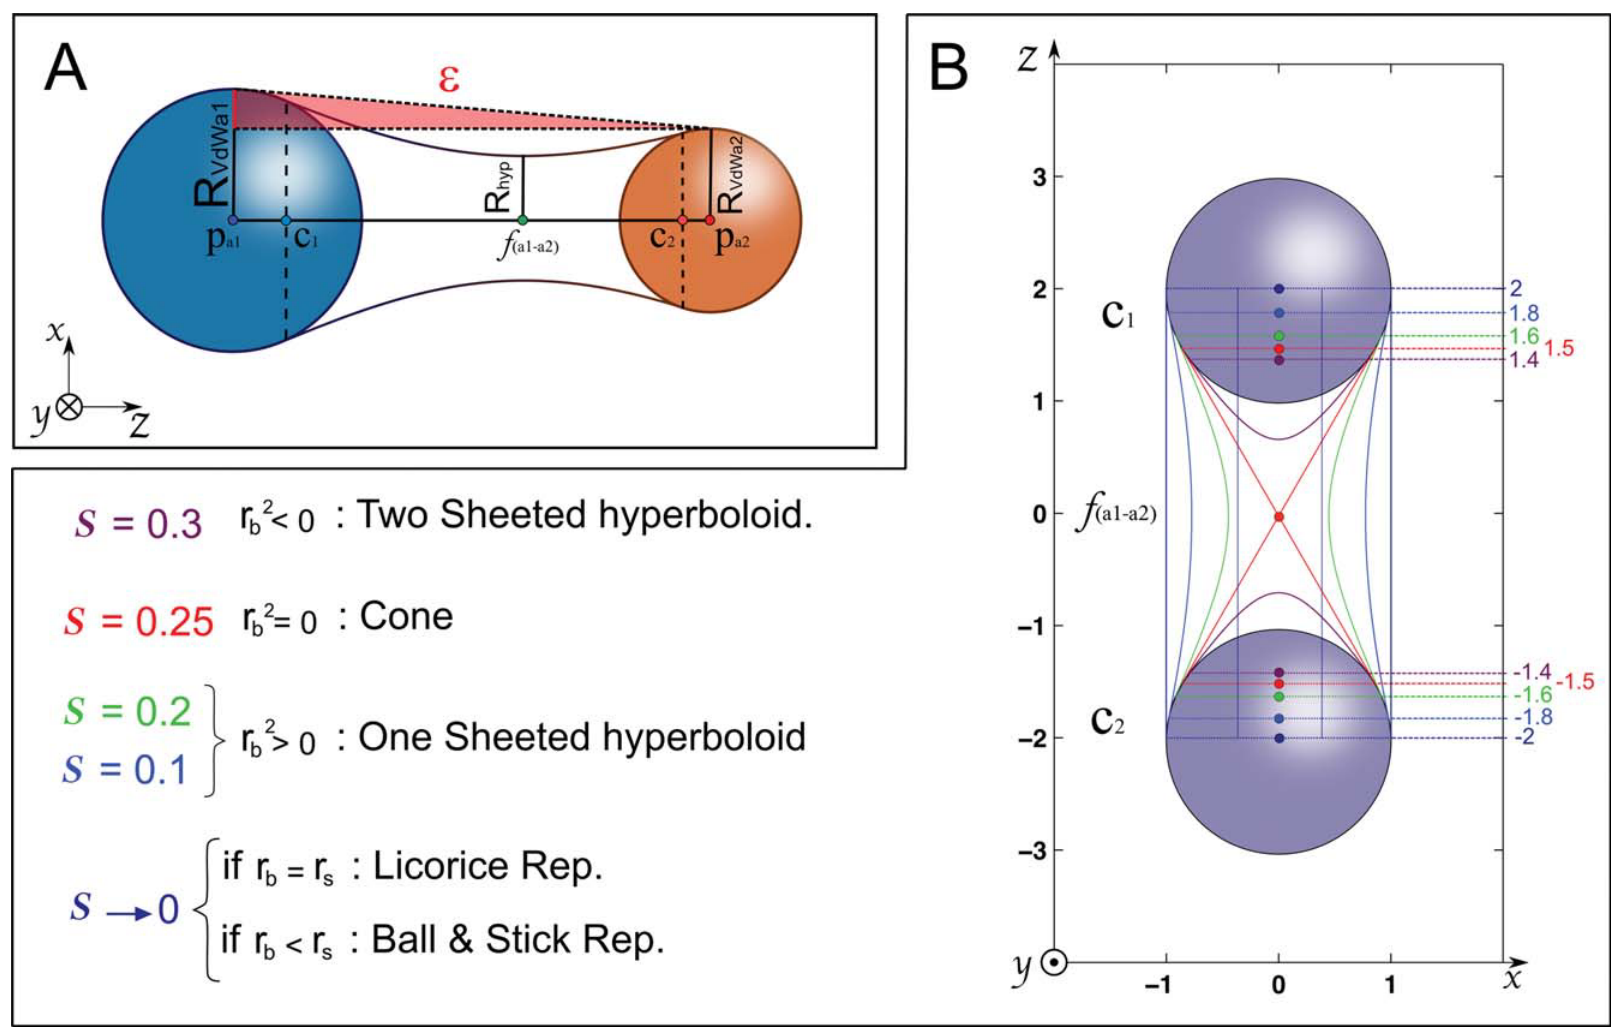
\includegraphics[width=\textwidth]{figures/ch1/hyperballs}
    	\caption{\emph{Hyperballs}. La figure A représente une paire d'atomes liés, avec quelques-uns des paramètres utilisés pour la représentation analytique de ce système. La figure B illustre particulièrement l'effet du \emph{shrink factor} (noté $S$), le principal paramètre d'ajustement de la forme de la liaison, du rayon de la liaison $r_{b}$ et du rayon des sphères $r_{b}$ (ici identique pour les deux sphères. On constante que lorsque le \emph{shrink factor} devient grand (supérieur à $0,3$ pour les valeurs de cet exemple), l'hyperboloïde qui représente la liaison entre les deux atomes se sépare en deux \emph{nappes}. Cet effet est avantageux si l'on souhaite représenter la rupture d'une liaison covalente ou hydrogène. Pour des valeurs de \emph{shrink factor} plus faibles, l'hyperboloïde reste unifiée mais apparaît plus ou moins \og creusée \fg{}. Lorsque le \emph{shrink} factor est nul, la liaison est représentée par un cylindre. Dans ce dernier cas, si le rayon des sphères est supérieur au rayon des liaisons, les \emph{Hyperballs} présentent l'apparence d'une représentation en boules et bâtons ; si le rayon est identique, alors elles génèrent une représentation à bâtons, ou \og en réglisse \fg{}. Dans tous les cas, elles le font avec un nombre de triangles très réduit, et d'excellentes performances. Surtout, ces paramètres étant modifiables à volonté et même en temps réel, les \emph{Hyperballs} permettent de basculer progressivement d'un mode de représentation à un autre. Crédit :~\cite{chavent2011gpu}.}
   		\label{fig:hyperballs}
    \end{figure}
		
	\paragraph{Structures secondaires.} En biologie structurale, on appelle structure secondaire~\cite{foltmann1981protein} la structure tridimensionnelle localement adoptée par un segment de molécule (généralement de protéine). Cette structure secondaire est définie par les liaisons hydrogène au sein du segment concerné, plus précisément entre les groupements amide et carbonyle du squelette peptidique, dans le cas des protéines, et entre les bases nucléiques dans le cas des acides nucléiques (acide désoxyribonucléique, ou ADN, et acide ribonucléique, ou ARN). Parfois, cette définition est assouplie et un segment peut être considéré comme une structure secondaire particulière sur la base des valeurs de certains de ses angles dièdres, indépendamment des liaisons hydrogène. Les algorithmes couramment utilisés pour identifier les structures secondaires incluent DSSP~\cite{kabsch1983dictionary}, \emph{Define}~\cite{richards1988identification}, \emph{Stride}~\cite{frishman1995knowledge} et SST~\cite{konagurthu2012minimum}.
		
	Dans la majorité des cas, une structure secondaire est soit une hélice alpha, soit un feuillet bêta~\cite{pauling1951structure}. Dans une représentation dite \og en structures secondaires \fg{} ces segments de molécule sont remplacés par des représentations plus schématiques. Un exemple pour une hélice alpha est présenté dans la figure~\ref{fig:aHelix}, et un exemple pour un feuillet bêta est fourni sur la figure~\ref{fig:bSheet}. L'utilisation de ces schématisations permet de considérablement simplifier la représentation de la molécule finale, comme l'illustre la figure~\ref{fig:4awn_ss}.
		
	De plus, ces représentations schématiques correspondent à des critères physico-chimiques précis et pertinents pour l'analyse des molécules concernées. La représentation en structures secondaires permet donc de simplifier la représentation tout en communicant efficacement des informations précises sur la molécule affichée~\cite{richardson2002teaching}. Le nombre d'objets différents (et de triangles, si des maillages sont utilisés) et très fortement réduit, ce qui améliore les performances d'affichage. Surtout, la molécule devient plus facile à observer, sa structure est plus lisible, et le niveau d'occultation des zones internes ou en arrière-plan de la molécule est considérablement diminué.
		
	Toutefois, l'utilisation de cette technique de visualisation implique une perte d'information. En effet, les atomes ne sont plus visibles, aussi la composition précise de la molécule n'est-elle plus perceptible. De fait, il devient difficile d'apprécier certaines propriétés du système, comme les champs électrostatiques, l'hydrophobicité, les cavités de la surface moléculaire et autres zones susceptibles de faciliter les interactions avec d'autres molécules. Il est cependant possible de représenter certaines de ces propriétés par des couleurs, par exemple.
		
	La représentation en structures secondaires est très courante, notamment pour visualiser des trajectoires\footnote{Dans le contexte de la dynamique moléculaire, on appelle \og trajectoire \fg{} l'évolution du système dans le temps, en particulier l'évolution des positions et des vélocités des particules simulées.} de dynamique moléculaire. Cette raison suffit à en faire une application majeure pour une technique de sélection de cibles mobiles. Le niveau d'occultation est particulièrement faible (relativement aux autres représentations, mais il reste élevé dans l'absolu) et les cibles, assez grosses, bougent relativement peu.
		
	Cependant, en pratique, il est courant d'associer à une représentation en structures secondaires la représentation \og tout atome \fg{} d'une partie de la molécule, généralement la partie qu'on soupçonne d'interagir avec une autre molécule, d'être un site d'arrimage, ou de présenter un autre intérêt particulier. Il en résulte une situation hybride, avec des cibles très mobiles et petites, mais un degré d'occultation global réduit. Cela permet de réduire le nombre de cibles potentielles, mais ce n'est possible qu'à condition de savoir \emph{a priori} qu'un sous-ensemble d'atomes --- et seulement ce sous-ensemble --- est susceptible d'être choisi par l'utilisateur, ce qui n'est pas toujours possible. La figure~\ref{fig:myoglobin} est un exemple de cette représentation hybride.
		
	\begin{figure}[H]
		\centering
		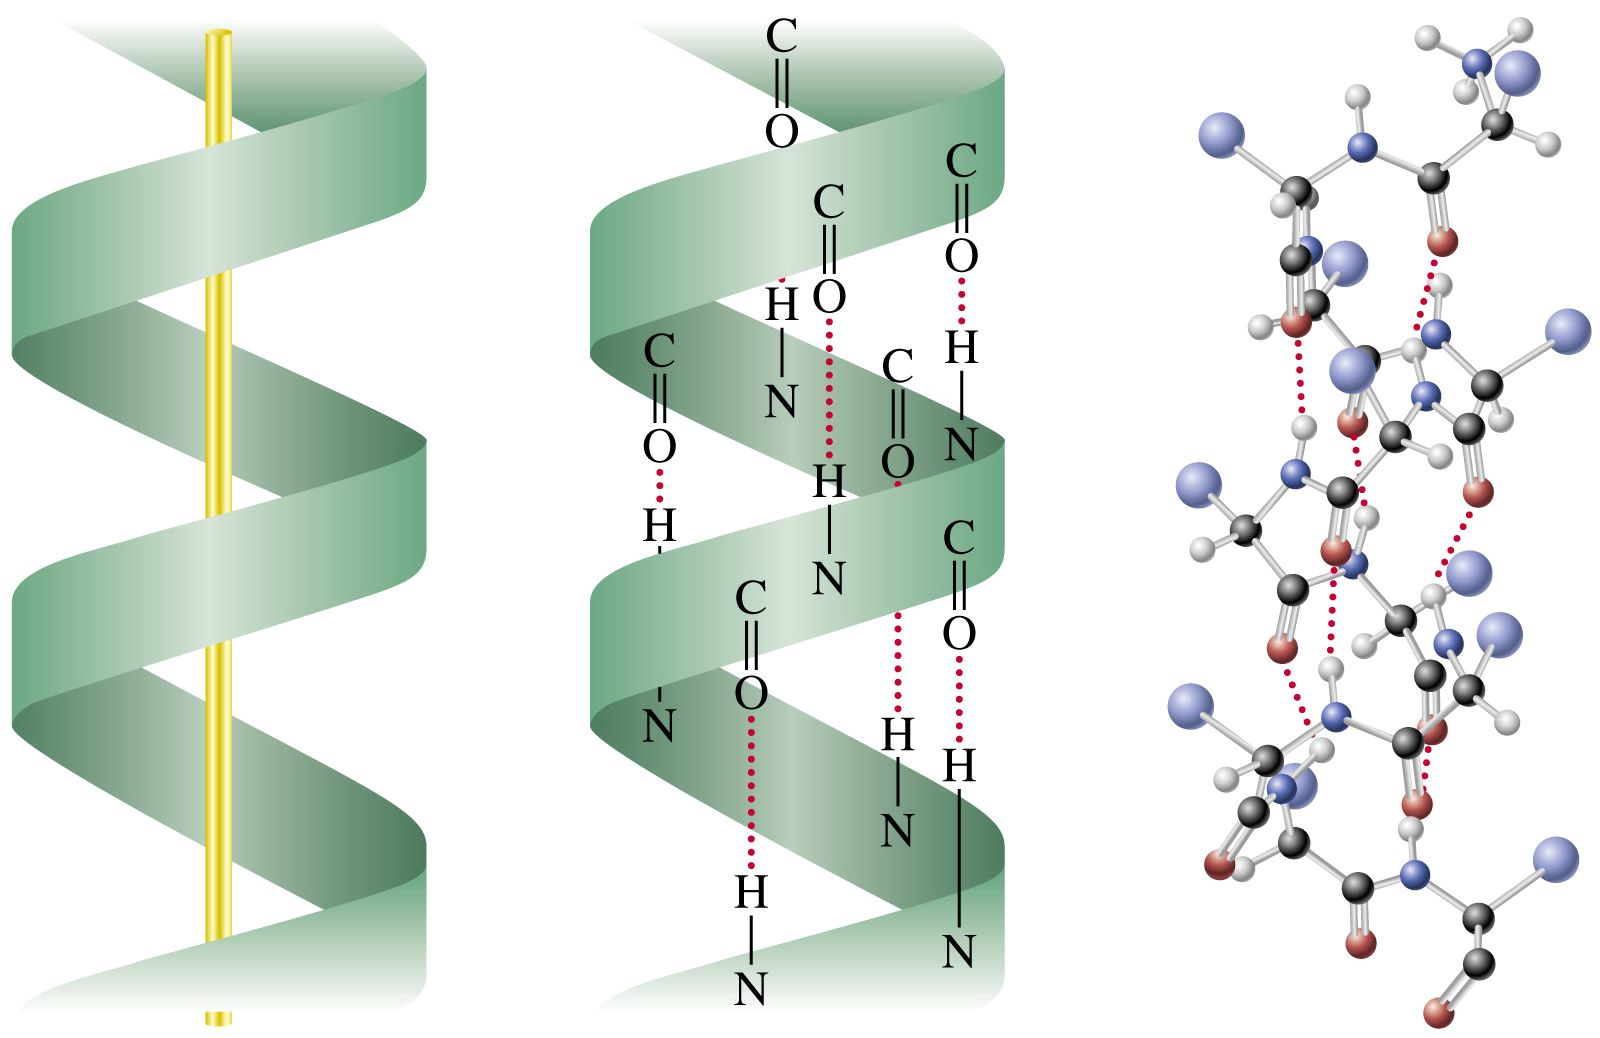
\includegraphics[width=\textwidth]{figures/ch1/aHelix}
		\caption[Hélices alpha, trois représentations différentes.]{Une hélice alpha sous forme schématique (à gauche), sous forme schématique avec un affichage texte représentant les atomes de façon simplifiée (au centre) et en représentation \og tout atome \fg{} (à droite) avec les doubles liaisons illustrées explicitement par deux bâtons, et les liaisons hydrogène représentées en pointillés rouges. Lors d'un affichage \og en structures secondaires \fg{} la représentation de gauche est généralement choisie, la plupart du temps sans la tige jaune au niveau de l'axe de l'hélice. Crédit : \emph{\emph{Bioinformatics -- An Introduction}, Bioinformatics Lab, Anna University - K.~B. Chandrasekhar Research Centre, Madras Institute of Technology}\footnotemark.}
		\label{fig:aHelix}
	\end{figure}
	
	\footnotetext{\url{http://bioinfo.au-kbc.org.in/books/bi/1.html}}
		
	\begin{figure}[H]
		\centering
		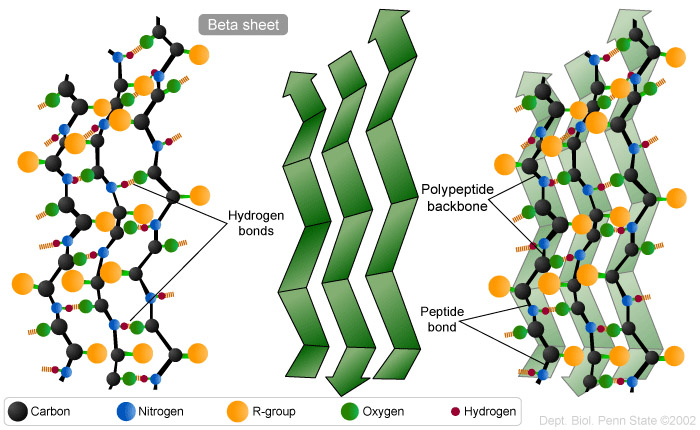
\includegraphics[width=\textwidth]{figures/ch1/bSheet}
		\caption{Un feuillet bêta en représentation \og tout atome \fg{} (à gauche), sous forme schématique (au milieu), et en représentation \og tout atome \fg{} mixte (à droite). Lors d'un affichage \og en structures secondaires \fg{} la représentation du milieu est généralement choisie. Crédit : \emph{Department of Biology -- Penn State University.}\protect\footnotemark}
		\label{fig:bSheet}
	\end{figure}
		\footnotetext{\url{https://wikispaces.psu.edu/display/Biol230WCE/Properties+of+Macromolecules+I-Proteins}}
		
	\begin{figure}[H]
		\centering
		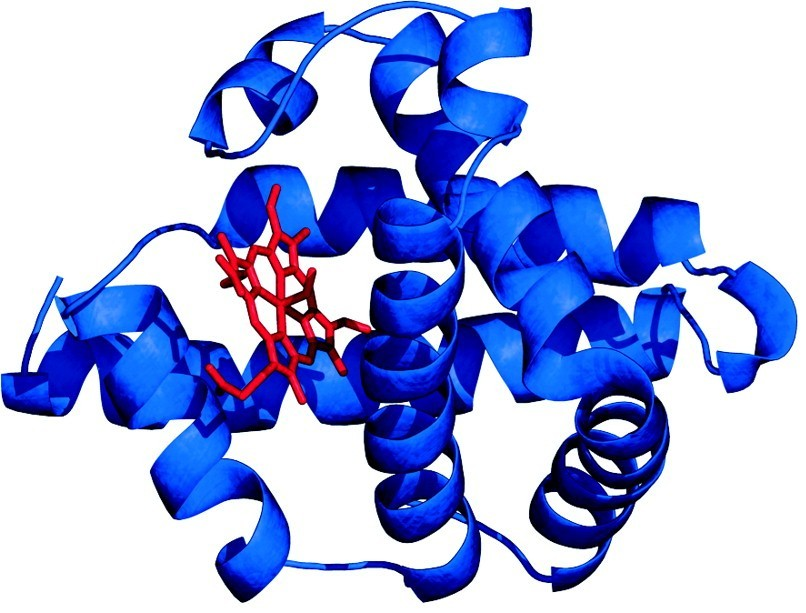
\includegraphics[width=\textwidth]{figures/ch1/myoglobin}
		\caption{À gauche : représentation en structures secondaires d'une molécule de myoglobine, une métalloprotéine présente dans les muscles des vertébrés, et dont la fonction est de stocker le dioxygène ; son hème --- un cofacteur contenant un atome de fer et pouvant accueillir du dioxygène --- est représenté en \og tout atome \fg{} et plus précisément en bâtons. À droite : une représentation schématique du hème et des histidines qui le stabilisent. Crédit :~\cite{Ordway3441}}
		\label{fig:myoglobin}
	\end{figure}
	
	Dans la littérature anglo-saxonne, la représentation en structures secondaires est parfois appelée \emph{cartoon} ou \emph{ribbons}~\cite{carson1986algorithm, richardson2000early}.
		
		
	\paragraph{Surface accessible au solvant et surface de Connolly.} Plutôt que de représenter les atomes d'une molécule, ou ses liaisons covalentes, ou sa structure interne de façon schématique, il est possible de représenter sa \og surface \fg{}. Attendu qu'une molécule n'est pas un objet macroscopique, le concept de surface est nécessairement plus abstrait, et il convient donc de préciser de quoi il s'agit. On peut en effet définir la surface moléculaire de plusieurs façons.
		
	Un définition très courante est la surface de Connolly~\cite{connolly1983analytical}, parfois également appelée \emph{solvent excluded surface} dans la littérature anglo-saxonne. Il s'agit de l'ensemble des points auxquels la molécule et \og le solvant \fg{} (généralement une sphère représentant une molécule d'eau) peuvent entrer en contact, où le contact est défini par le rayon de van der Waals. La figure~\ref{fig:connolly} illustre plus clairement ce principe. Une autre surface très courante est la surface accessible au solvant~\cite{lee1971interpretation}, définie par l'ensemble des points parcouru par le centre de la sphère représentant le solvant quand elle est en contact avec la molécule. C'est également illustré par la figure~\ref{fig:connolly}. Enfin, la figure~\ref{fig:4awn_sas} montre une protéine entière représentée par sa surface accessible au solvant, et la figure~\ref{fig:4awn_ses} représente la surface de Connolly de cette protéine.
		
	\begin{figure}[H]
		\centering
		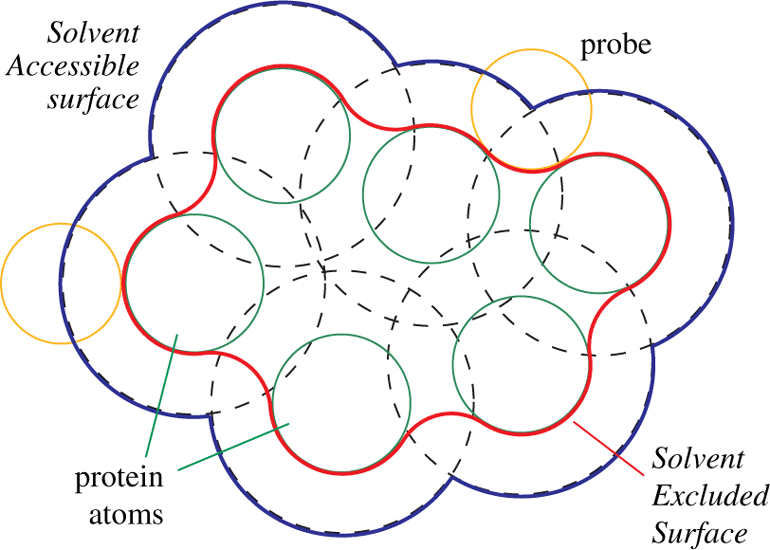
\includegraphics[width=\textwidth]{figures/ch1/connolly}
		\caption{Surface de Connolly d'une petite molécule. Six atomes sont représentés par des cercles verts correspondant à leurs rayons de van der Waals ; une sonde (\emph{probe}), i.e. le solvant, est représentée par un cercle jaune ; cette sonde est \og roulée \fg{} le long de la surface de la molécule, et son tracé est conservé en rouge : c'est la surface de Connolly. La surface tracée par le centre de la sonde est appelée surface accessible au solvant. Cet algorithme est couramment appelé \emph{rolling ball}~\cite{shrake1973environment}, et la surface de Connolly tire son nom des améliorations apportées par Michael Connolly à cet algorithme~\cite{connolly1983analytical, connolly1993molecular}. Crédit :~\cite{krone2009interactive}}
		\label{fig:connolly}
	\end{figure}
		
	\paragraph{Isosurface de densité.} On peut également représenter une molécule par sa surface en se basant sur un seuil de densité moléculaire. On calcule, dans une grille tridimensionnelle d'une résolution arbitraire, la densité en chaque case --- on construit un champ scalaire. Ensuite, on choisit arbitrairement un seuil de densité, et l'on trace une isosurface de densité à partir de ce seuil. On utilise généralement pour ce faire l'algorithme des \emph{marching cubes}~\cite{lorensen1987marching}, illustré par la figure~\ref{fig:marchingCubes}. L'isosurface de densité $D$ correspond à l'ensemble des points de l'espace dont la densité moléculaire vaut $D$.
		
	Les figures~\ref{fig:4awn_iso_0_2}, \ref{fig:4awn_iso_0_5}, \ref{fig:4awn_iso_1_0} et~\ref{fig:4awn_iso_1_5} représentent des isosurfaces de densité avec des valeurs de $D$ plus ou moins élevées ($0,2$, $0,5$, $1,0$ et $1,5$). Naturellement, plus la densité choisie est élevée, plus la surface sera proche des centres atomiques, et plus sa forme sera complexe, comme sur la figure~\ref{fig:4awn_iso_1_5} ; inversement, lorsque la densité est faible, la surface est loin des centres atomiques et sa forme est plus grossière, cf. la figure~\ref{fig:4awn_iso_0_2}.
	
	Outre le fait qu'elle représente une grandeur physique concrète, l'isosurface de densité a l'avantage d'être relativement rapide à calculer. En effet, l'algorithme \emph{QuickSurf}~\cite{krone2012fast, roberts2013lattice, stone2013early, stone2013gpu, stone2014gpu, sener2014visualization}, par exemple, permet de calculer une isosurface de densité suffisamment vite pour la recalculer en temps réel lors d'une simulation de dynamique moléculaire. Cet algorithme est conçu pour être exécuté sur un GPU (un processeur graphique, particulièrement adapté aux calculs très parallèles) ce qui améliore ses performances d'un à deux ordres de grandeur. Il permet de plus d'ajuster plusieurs paramètres : la résolution spatiale générale, le rayon des atomes (utilisé pour générer la grille de densité, par somme de gaussiennes 3D), l'isovaleur de densité voulue, la résolution de la grille de densité, et la distance de coupure utilisée pour la gaussienne associée à chaque atome\footnote{\url{http://www.ks.uiuc.edu/Research/vmd/current/ug/node73.html}}.
	
	Du fait des performances de cet algorithme et de sa souplesse, les isosurfaces de densité représentent un cas d'application intéressant. En effet, elles sont assez couramment utilisées en simulation de dynamique moléculaire, et présentent des caractéristiques très distinctes des modèles de représentation atomiques. Contrairement à ces derniers, elles ne présentent pas de (dizaines ou centaines) de milliers de cibles distinctes, mais un seul objet continu. De fait, au premier abord elles ne semblent pas nécessiter d'assistance à la sélection. Cependant, les nombreuses aspérités d'une isosurface, attendu qu'elles correspondent à celles de la molécule, peuvent être considérées comme des cibles distinctes, à condition d'avoir une méthode pour les distinguer. Cette méthode pourrait éventuellement être basée sur des critères de concavité et convexité. Si l'on considère chaque sous-ensemble convexe de la surface représentée sur la figure~\ref{fig:4awn_iso_1_5}, par exemple, on aboutit à plusieurs dizaines de cibles potentielles ; et ce pour une protéine de taille relativement réduite (moins de 2200 atomes, quand certaines protéines en comptent des dizaines de milliers). On peut également considérer les sous-ensembles concaves comme des cibles, car ils peuvent représenter des cavités ou tunnels\footnotemark dignes d'intérêt.
	
	\footnotetext{Les cavités et tunnels des protéines sont critiques pour la compréhension de phénomènes tels que la liaison de ligands, le transport moléculaire ou la catalyse enzymatique~\cite{paramo2014}.}
	
	On constate donc qu'une isosurface de densité peut présenter de nombreuses cibles mobiles, avec toutefois un niveau d'occultation réduit, puisque l'intérieur de la molécule n'est pas représenté. Les aspérités situées à \og l'arrière \fg{} de la molécule sont cependant totalement occultées. De plus, la représentation en isosurface est particulièrement prisée pour l'arrimage\footnote{\emph{docking}, en anglais} de protéines, qui implique au moins deux molécules et parfois beaucoup plus. Avec de nombreuses molécules, le nombre de cibles potentielles peut donc devenir très élevé, de même que la quantité de mouvement, puisqu'il faut ajouter au mouvement d'une aspérité d'une surface par rapport à elle-même le mouvement de toute la surface par rapport à l'environnement.
	
	\begin{figure}[H]
		\centering
		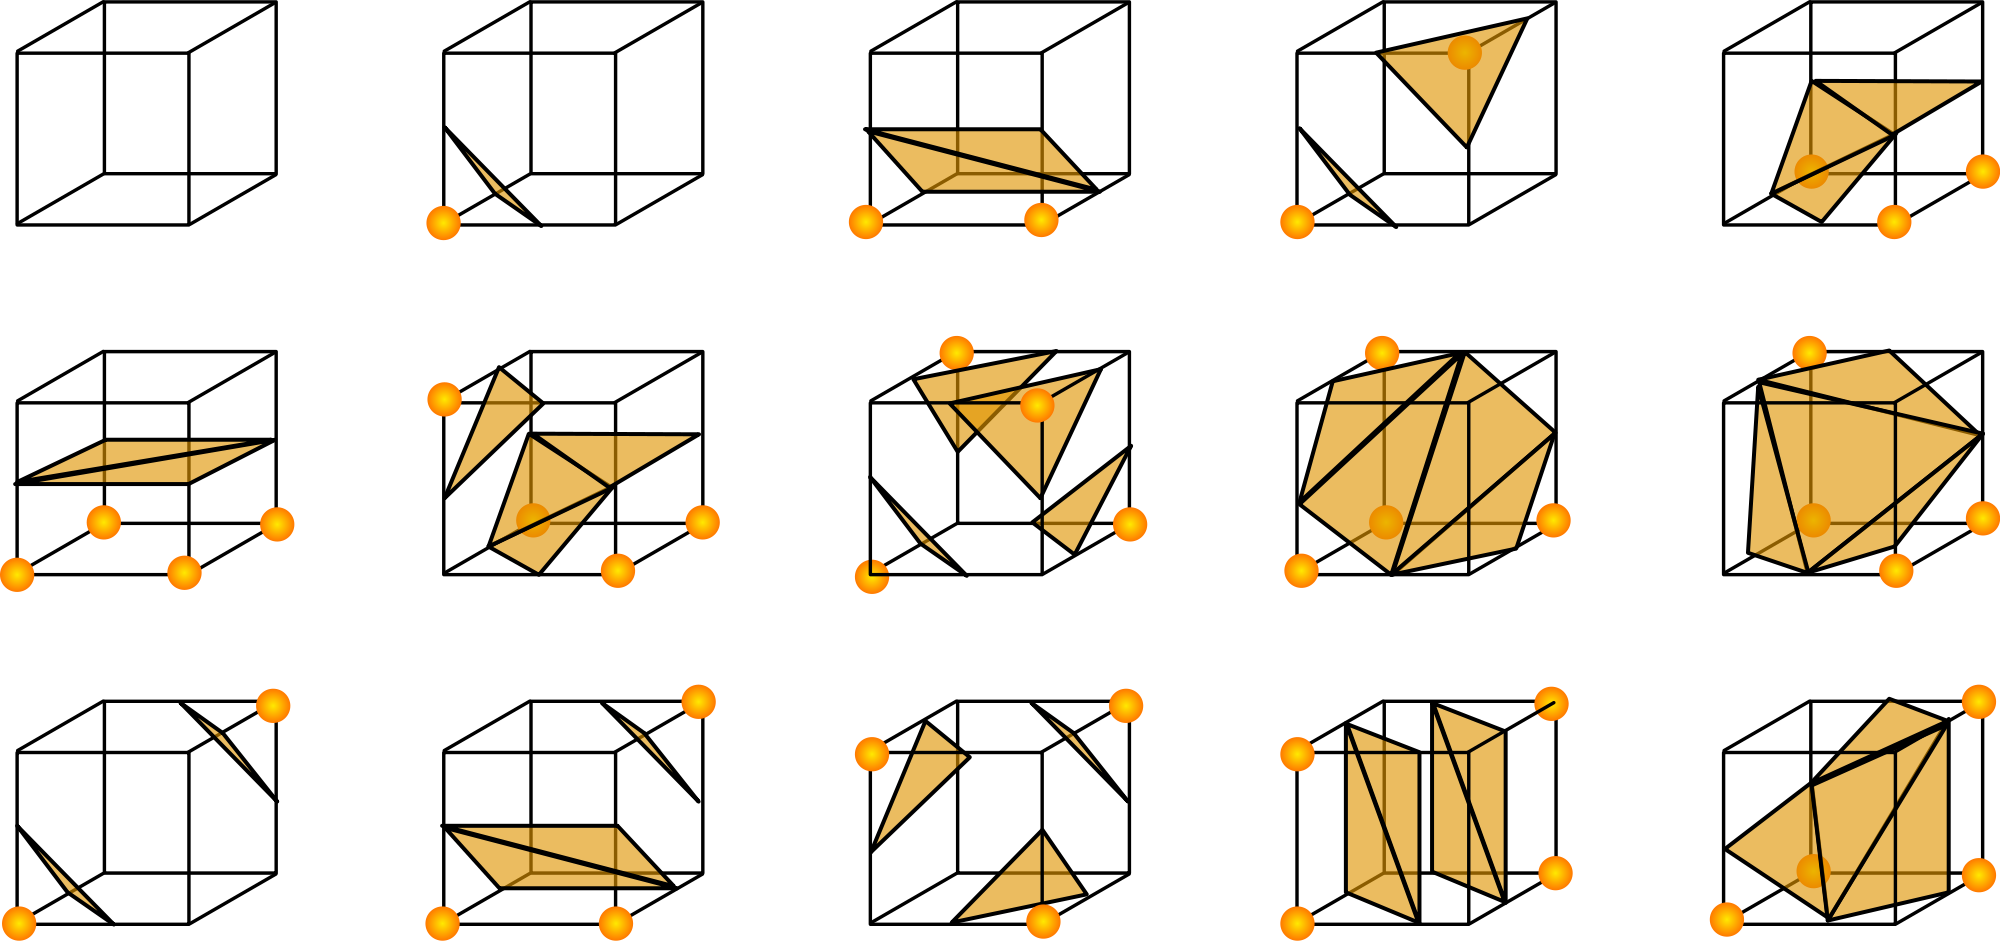
\includegraphics[width=\textwidth]{figures/ch1/marchingCubes}
		\caption{Dans l'algorithme des \emph{marching cubes}, lorsque l'on considère une cellule, on lit la valeur du champ scalaire aux huit sommets du cube. On choisit ensuite un des quinze cubes ci-dessus, en fonction des valeurs lues. L'opération est répétée pour chaque cellule de la grille, et les cubes forment un maillage de triangles. Crédit : \emph{Wikimedia}.}
		\label{fig:marchingCubes}
	\end{figure}
	
	\paragraph{Autres techniques de représentations.}
	La liste des techniques de représentation fournie ci-dessus ne saurait être considérée comme exhaustive. En effet, les logiciels de visualisation moléculaires sont nombreux, et les possibilités qu'ils offrent le sont encore plus. Des programmes courramment utilisés, tels que \emph{UnityMol}~\cite{doutreligne2014unitymol}, VMD~\cite{humphrey1996vmd}, \emph{PyMol}~\cite{delano2002pymol}, \emph{QuteMol}~\cite{tarini2006ambient, tarini2006qutemol}, \emph{Chimera}~\cite{pettersen2004ucsf}, ~\emph{Yasara}~\cite{krieger2014yasara}, \emph{LigandScout}~\cite{wolber2005ligandscout} ou \emph{Jmol}~\cite{herraez2006biomolecules} proposent des options très diverses. En outre, les divers modes de représentation proposés par ces outils peuvent être combinés librement, comme sur la figure~\ref{fig:transSS}.
	
	\begin{figure}[H]
		\centering
		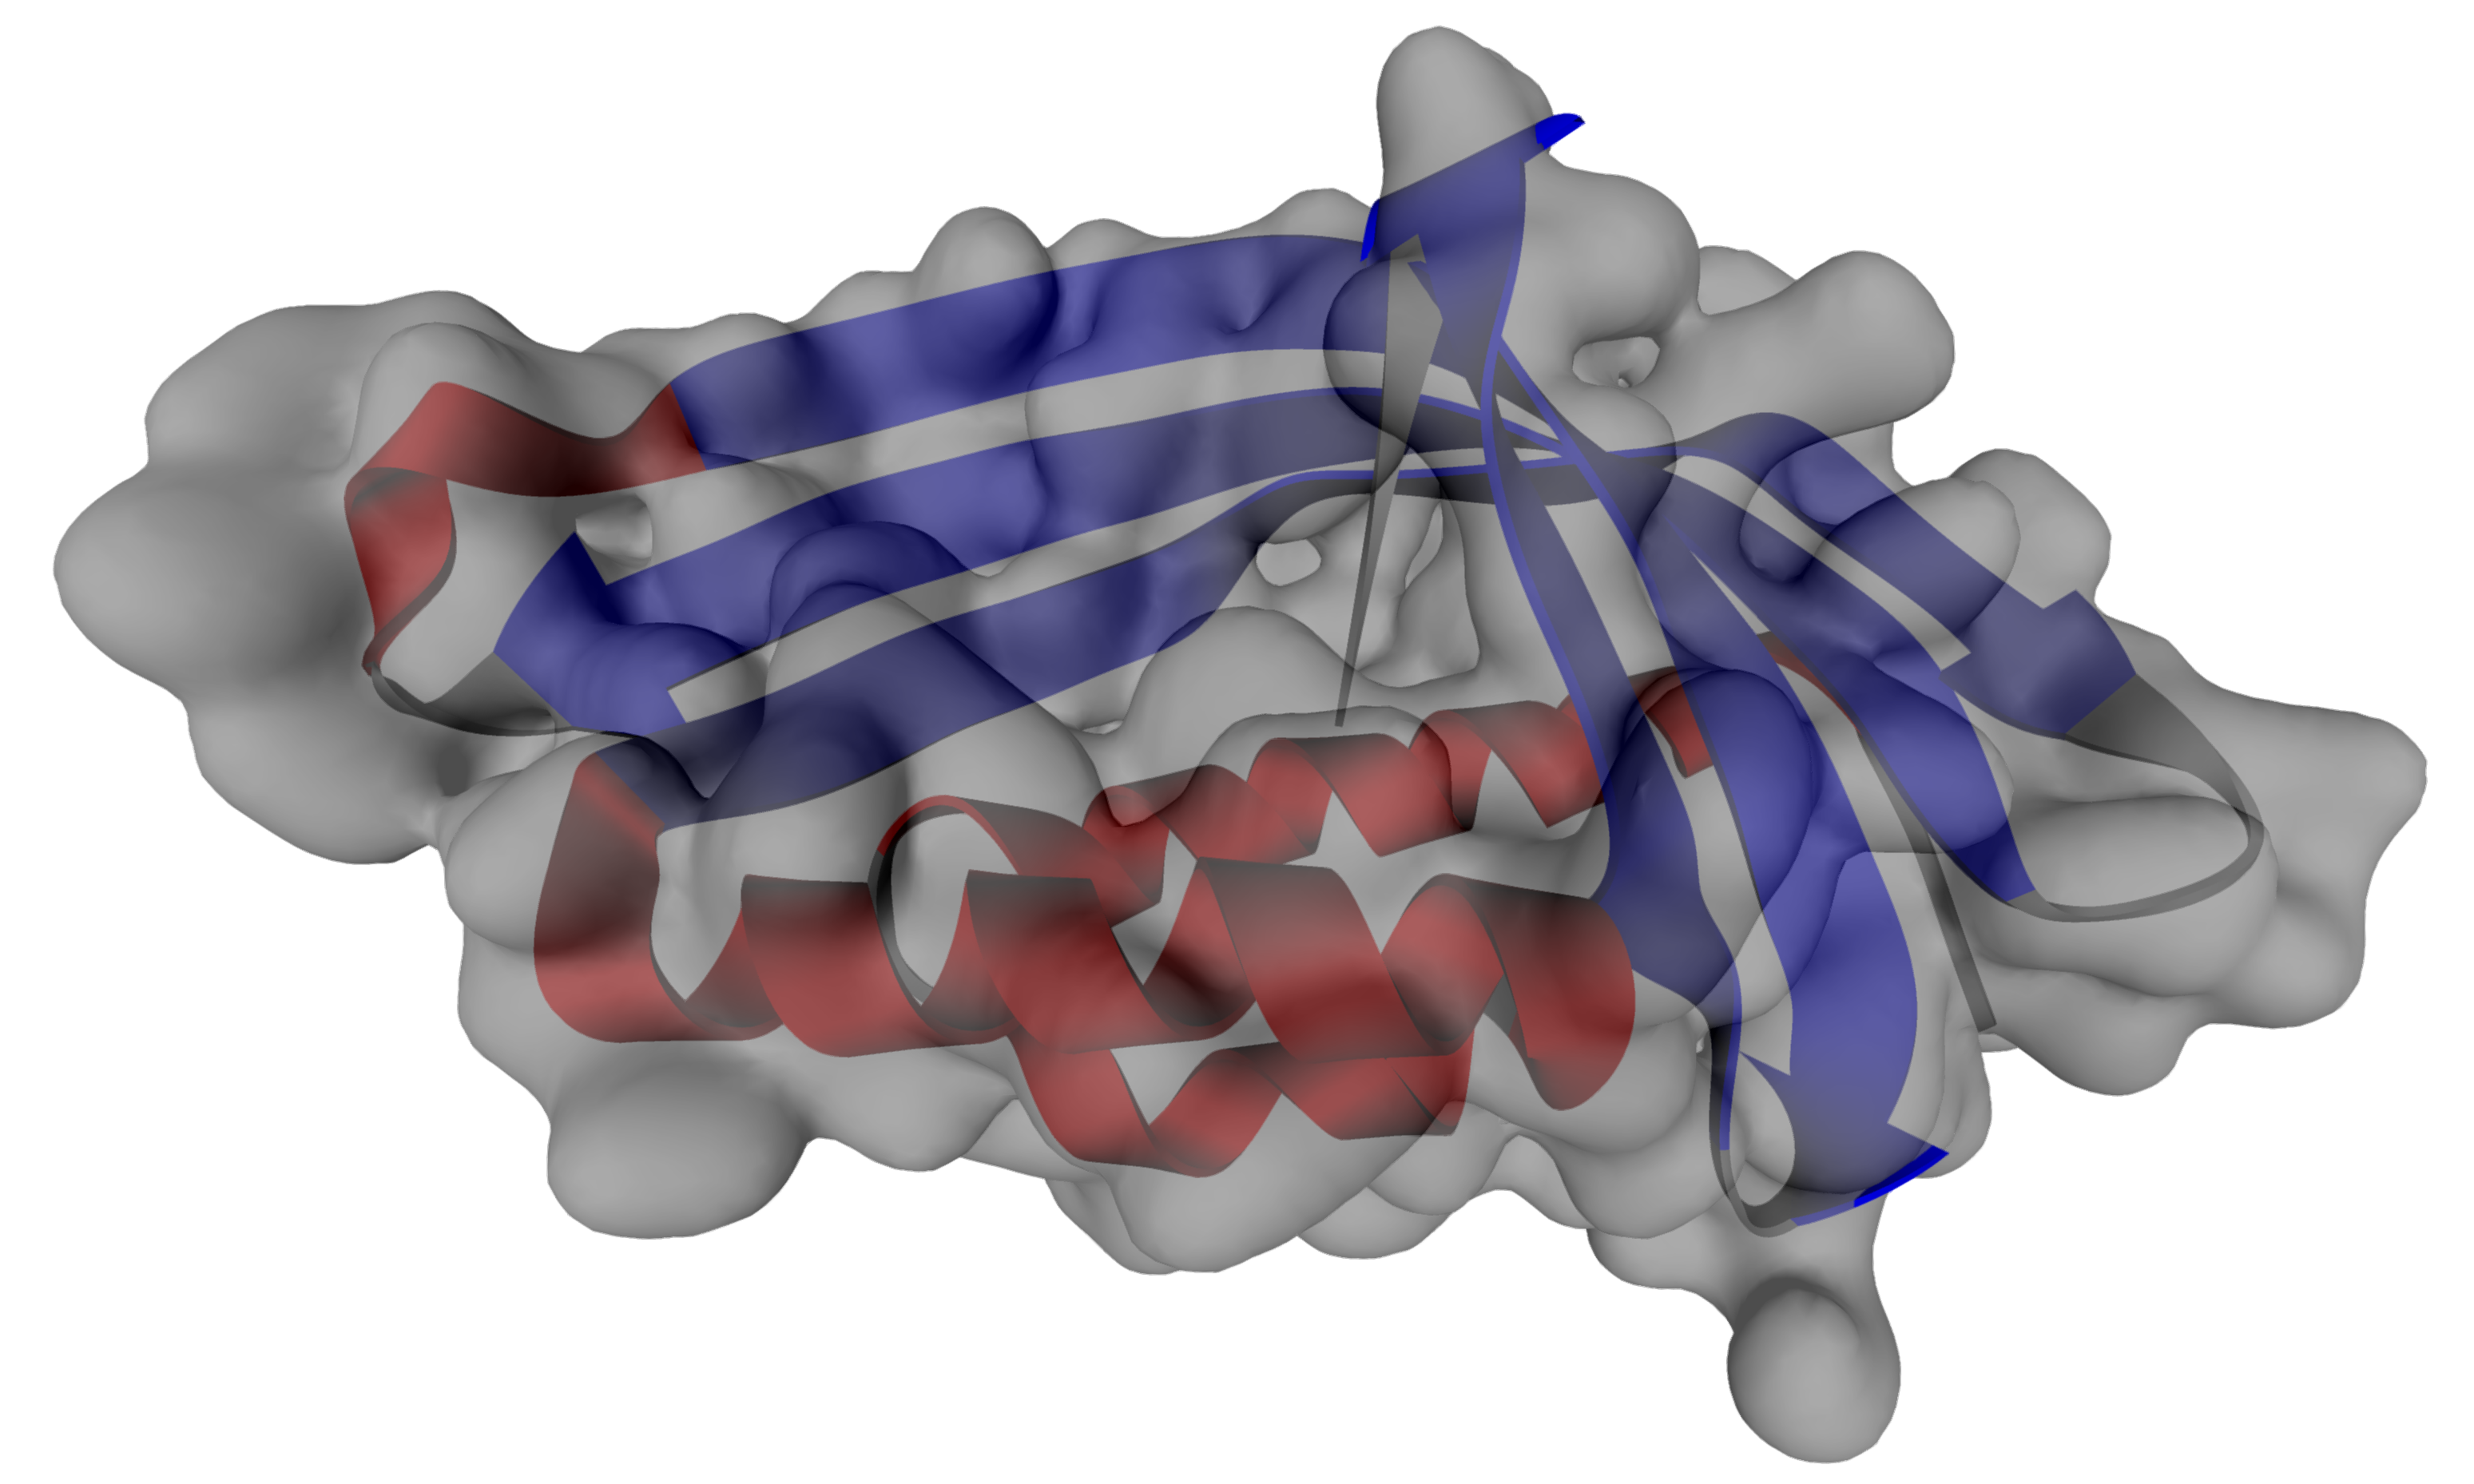
\includegraphics[width=\textwidth]{figures/ch1/transSS}
		\caption[Surface semi-transparente et structures secondaires.]{Illustration hybride d'une protéine de chloroplaste, représentée par une isosurface de densité semi-transparente et par ses structures secondaires. On peut donc apprécier à la fois le volume occupé par la molécule, les aspérités de sa surface, mais aussi sa structure interne et certaines de ses propriétés physico-chimiques. Illustration produite par \emph{UnityMol} à partir de la structure \emph{5HAD} de la \emph{Protein Data Bank}.}
		\label{fig:transSS}
	\end{figure}
	

		
	
	\begin{figure}[H]
		\centering
		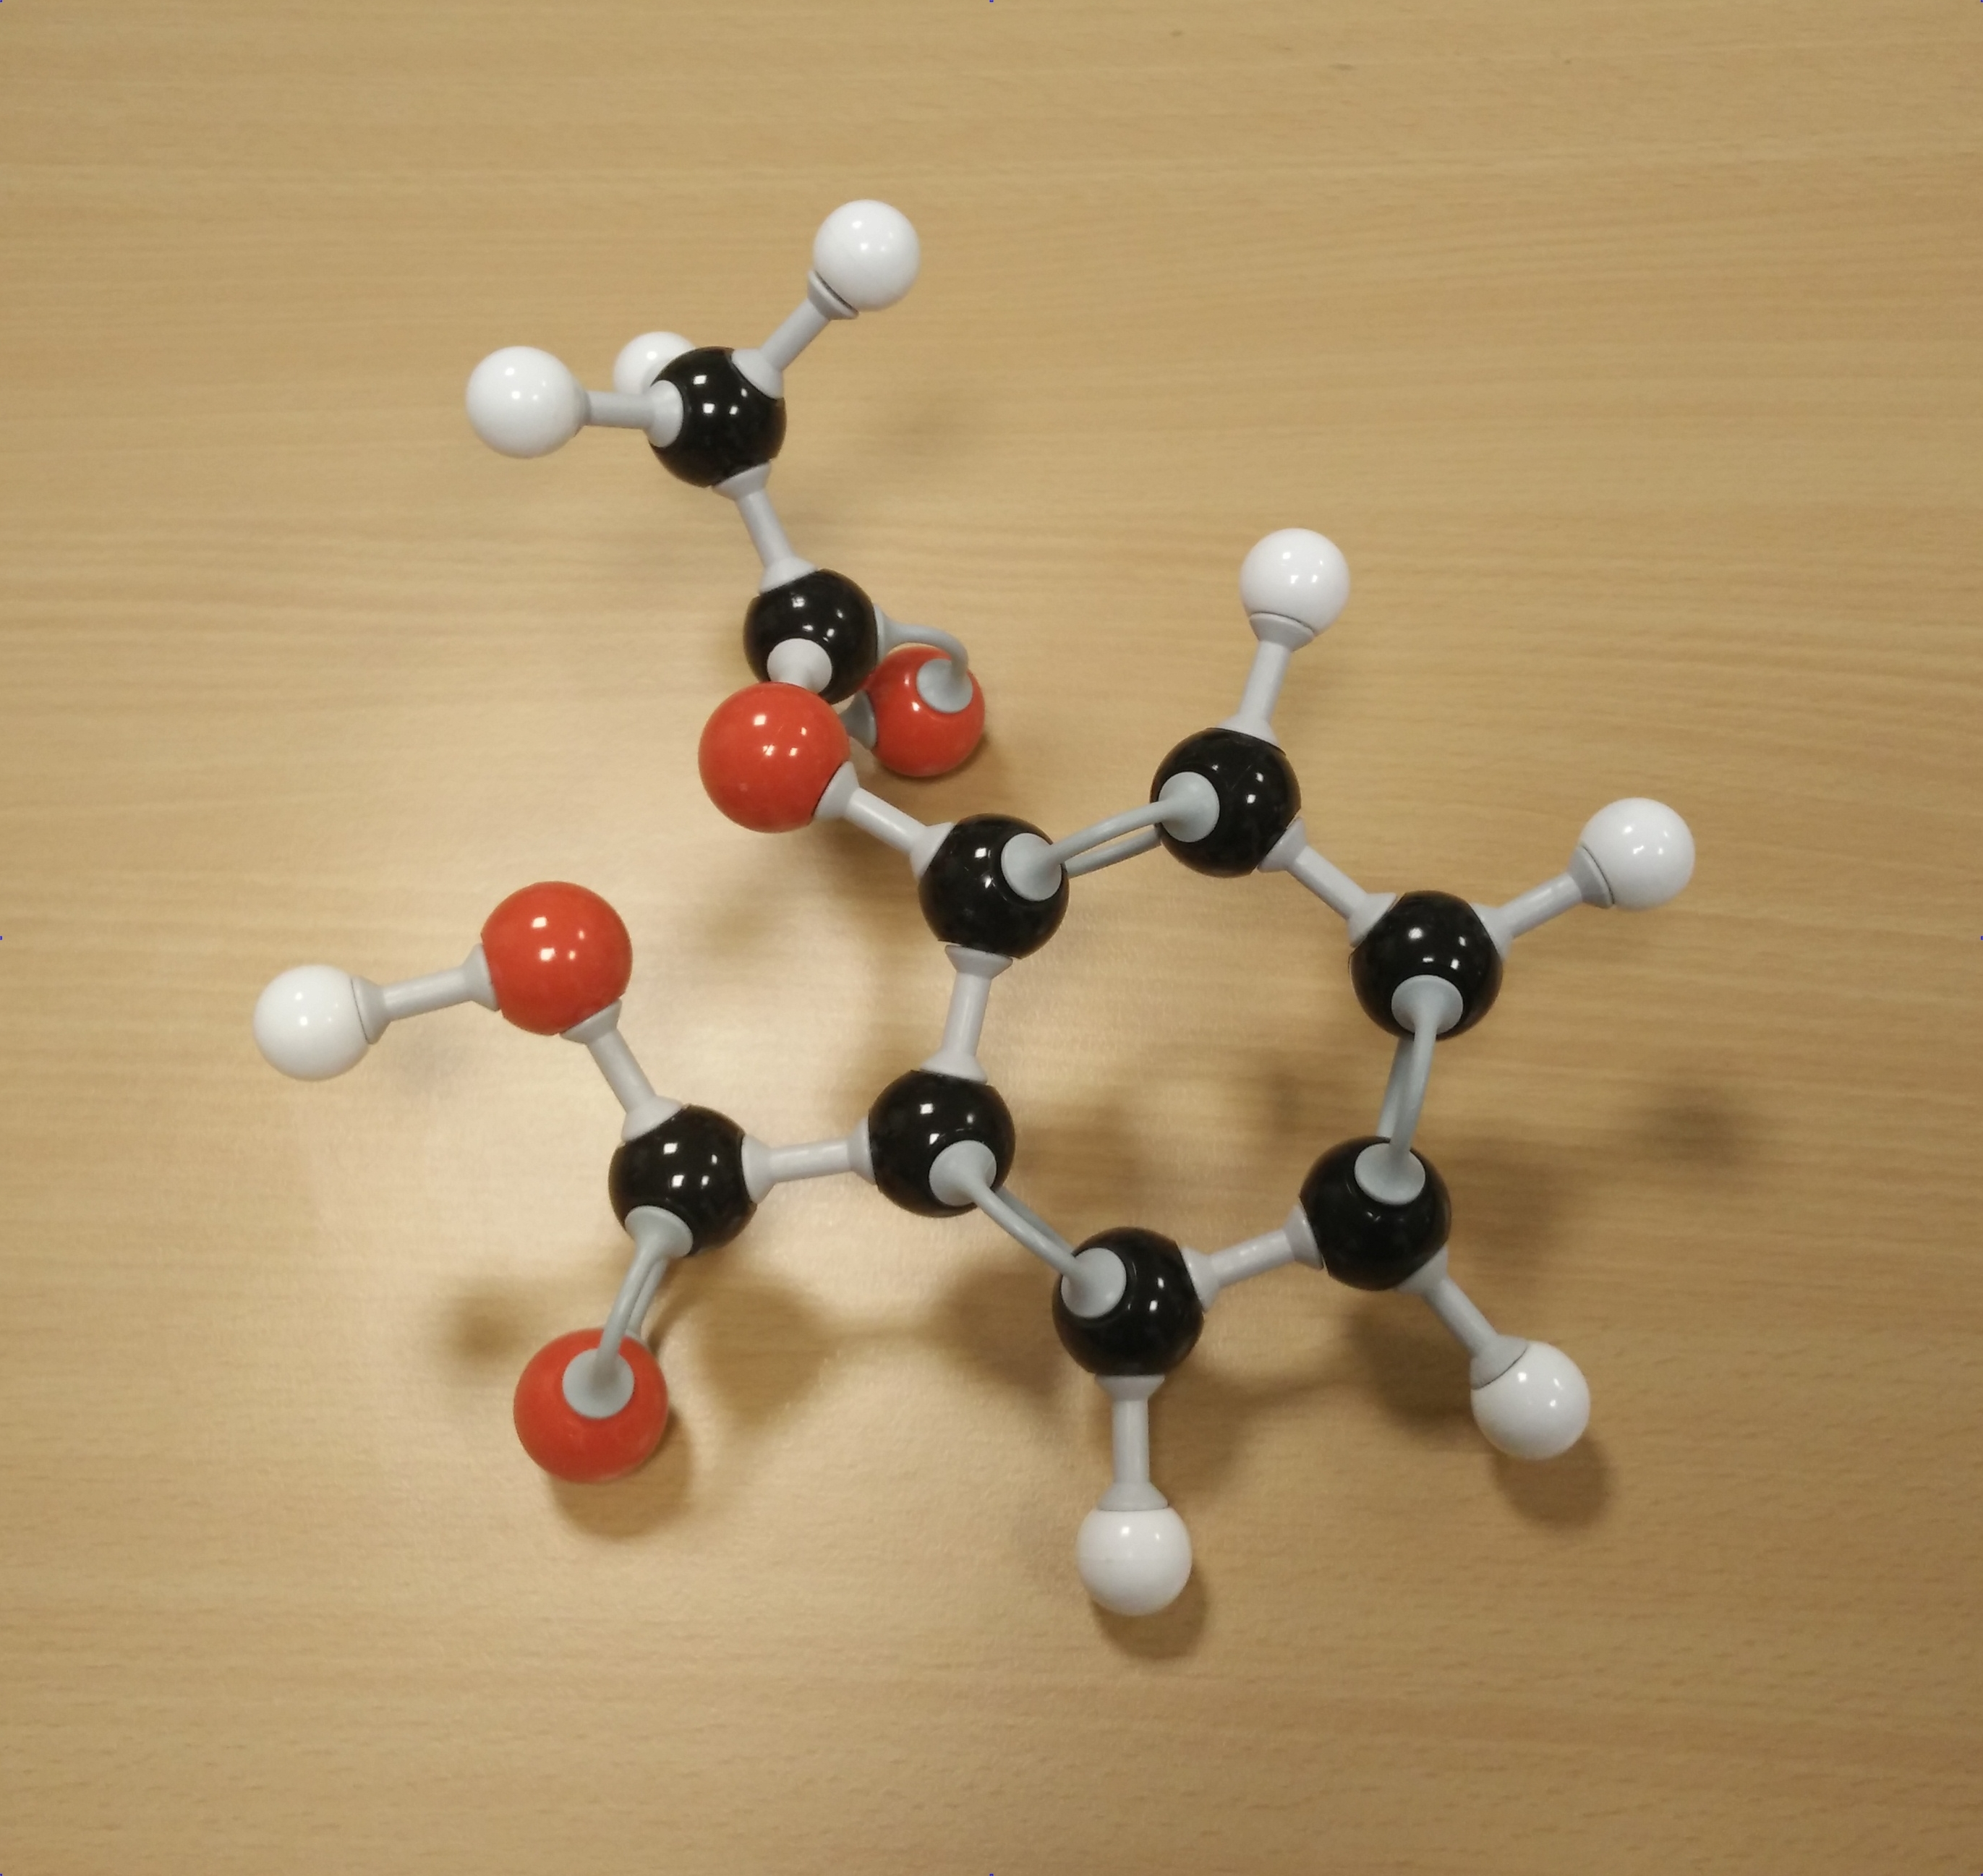
\includegraphics[width=\textwidth]{figures/ch1/aspirin}
		\caption{Modèle physique en boules et bâtons d'une molécule d'acide acétylsalicylique, plus connue sous le nom d'aspirine. Les liaisons covalentes sont représentées par des bâtons, et les liaisons doubles sont représentées par des paires de bâtons, ce qui permet notamment de rendre le modèle plus rigide à ces endroits-là, comme la molécule elle-même. La convention de couleurs CPK est respectée, donc le carbone est en noir, l'hydrogène en blanc, et l'oxygène en rouge. La manipulation manuelle de tels modèles peut favoriser la perception des propriétés d'une molécule, ou leur mémorisation.}
		\label{fig:aspirin}
	\end{figure}
	
	\newcommand{\subImgW}{0.5\textwidth}
	\begin{figure}[H]
		\begin{subfigure}[t]{\subImgW}
			\centering
			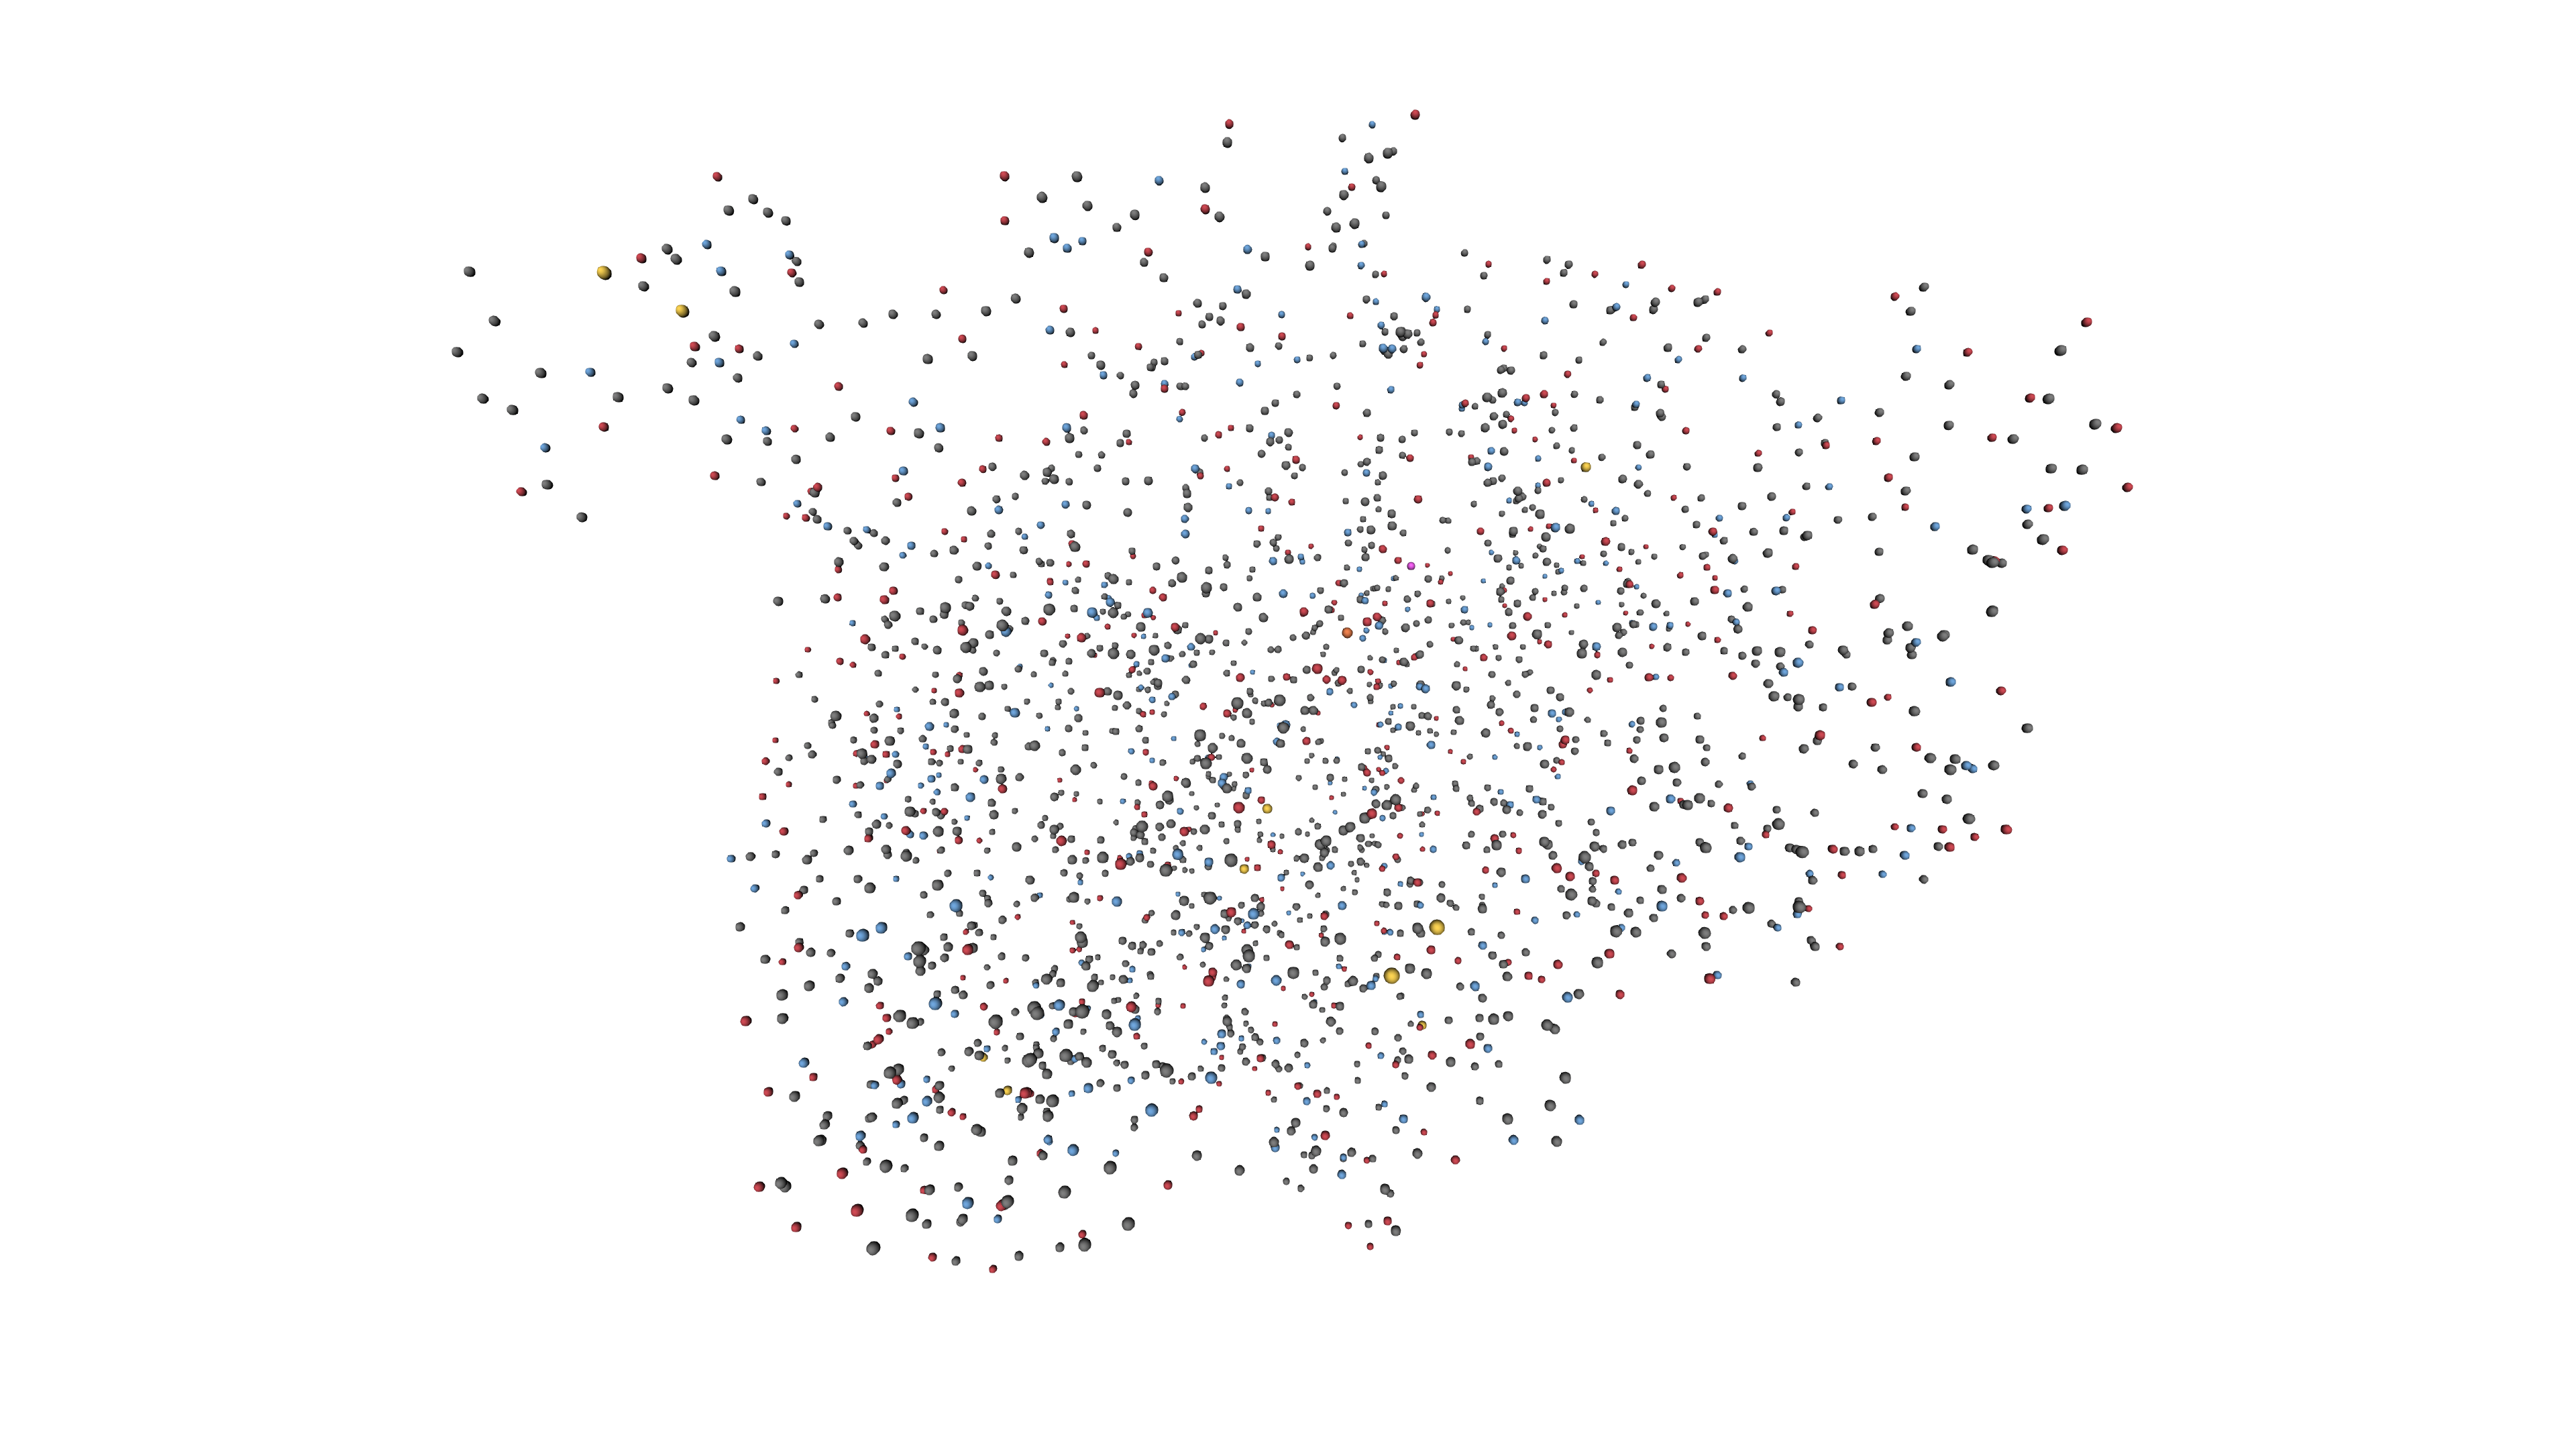
\includegraphics[width=\textwidth]{./figures/ch1/4awn_points}
			\caption{Représentation en \og points \fg{} ; seuls les atomes apparaissent.}
			\label{fig:4awn_points}
		\end{subfigure}
		~
		\begin{subfigure}[t]{\subImgW}
			\centering
			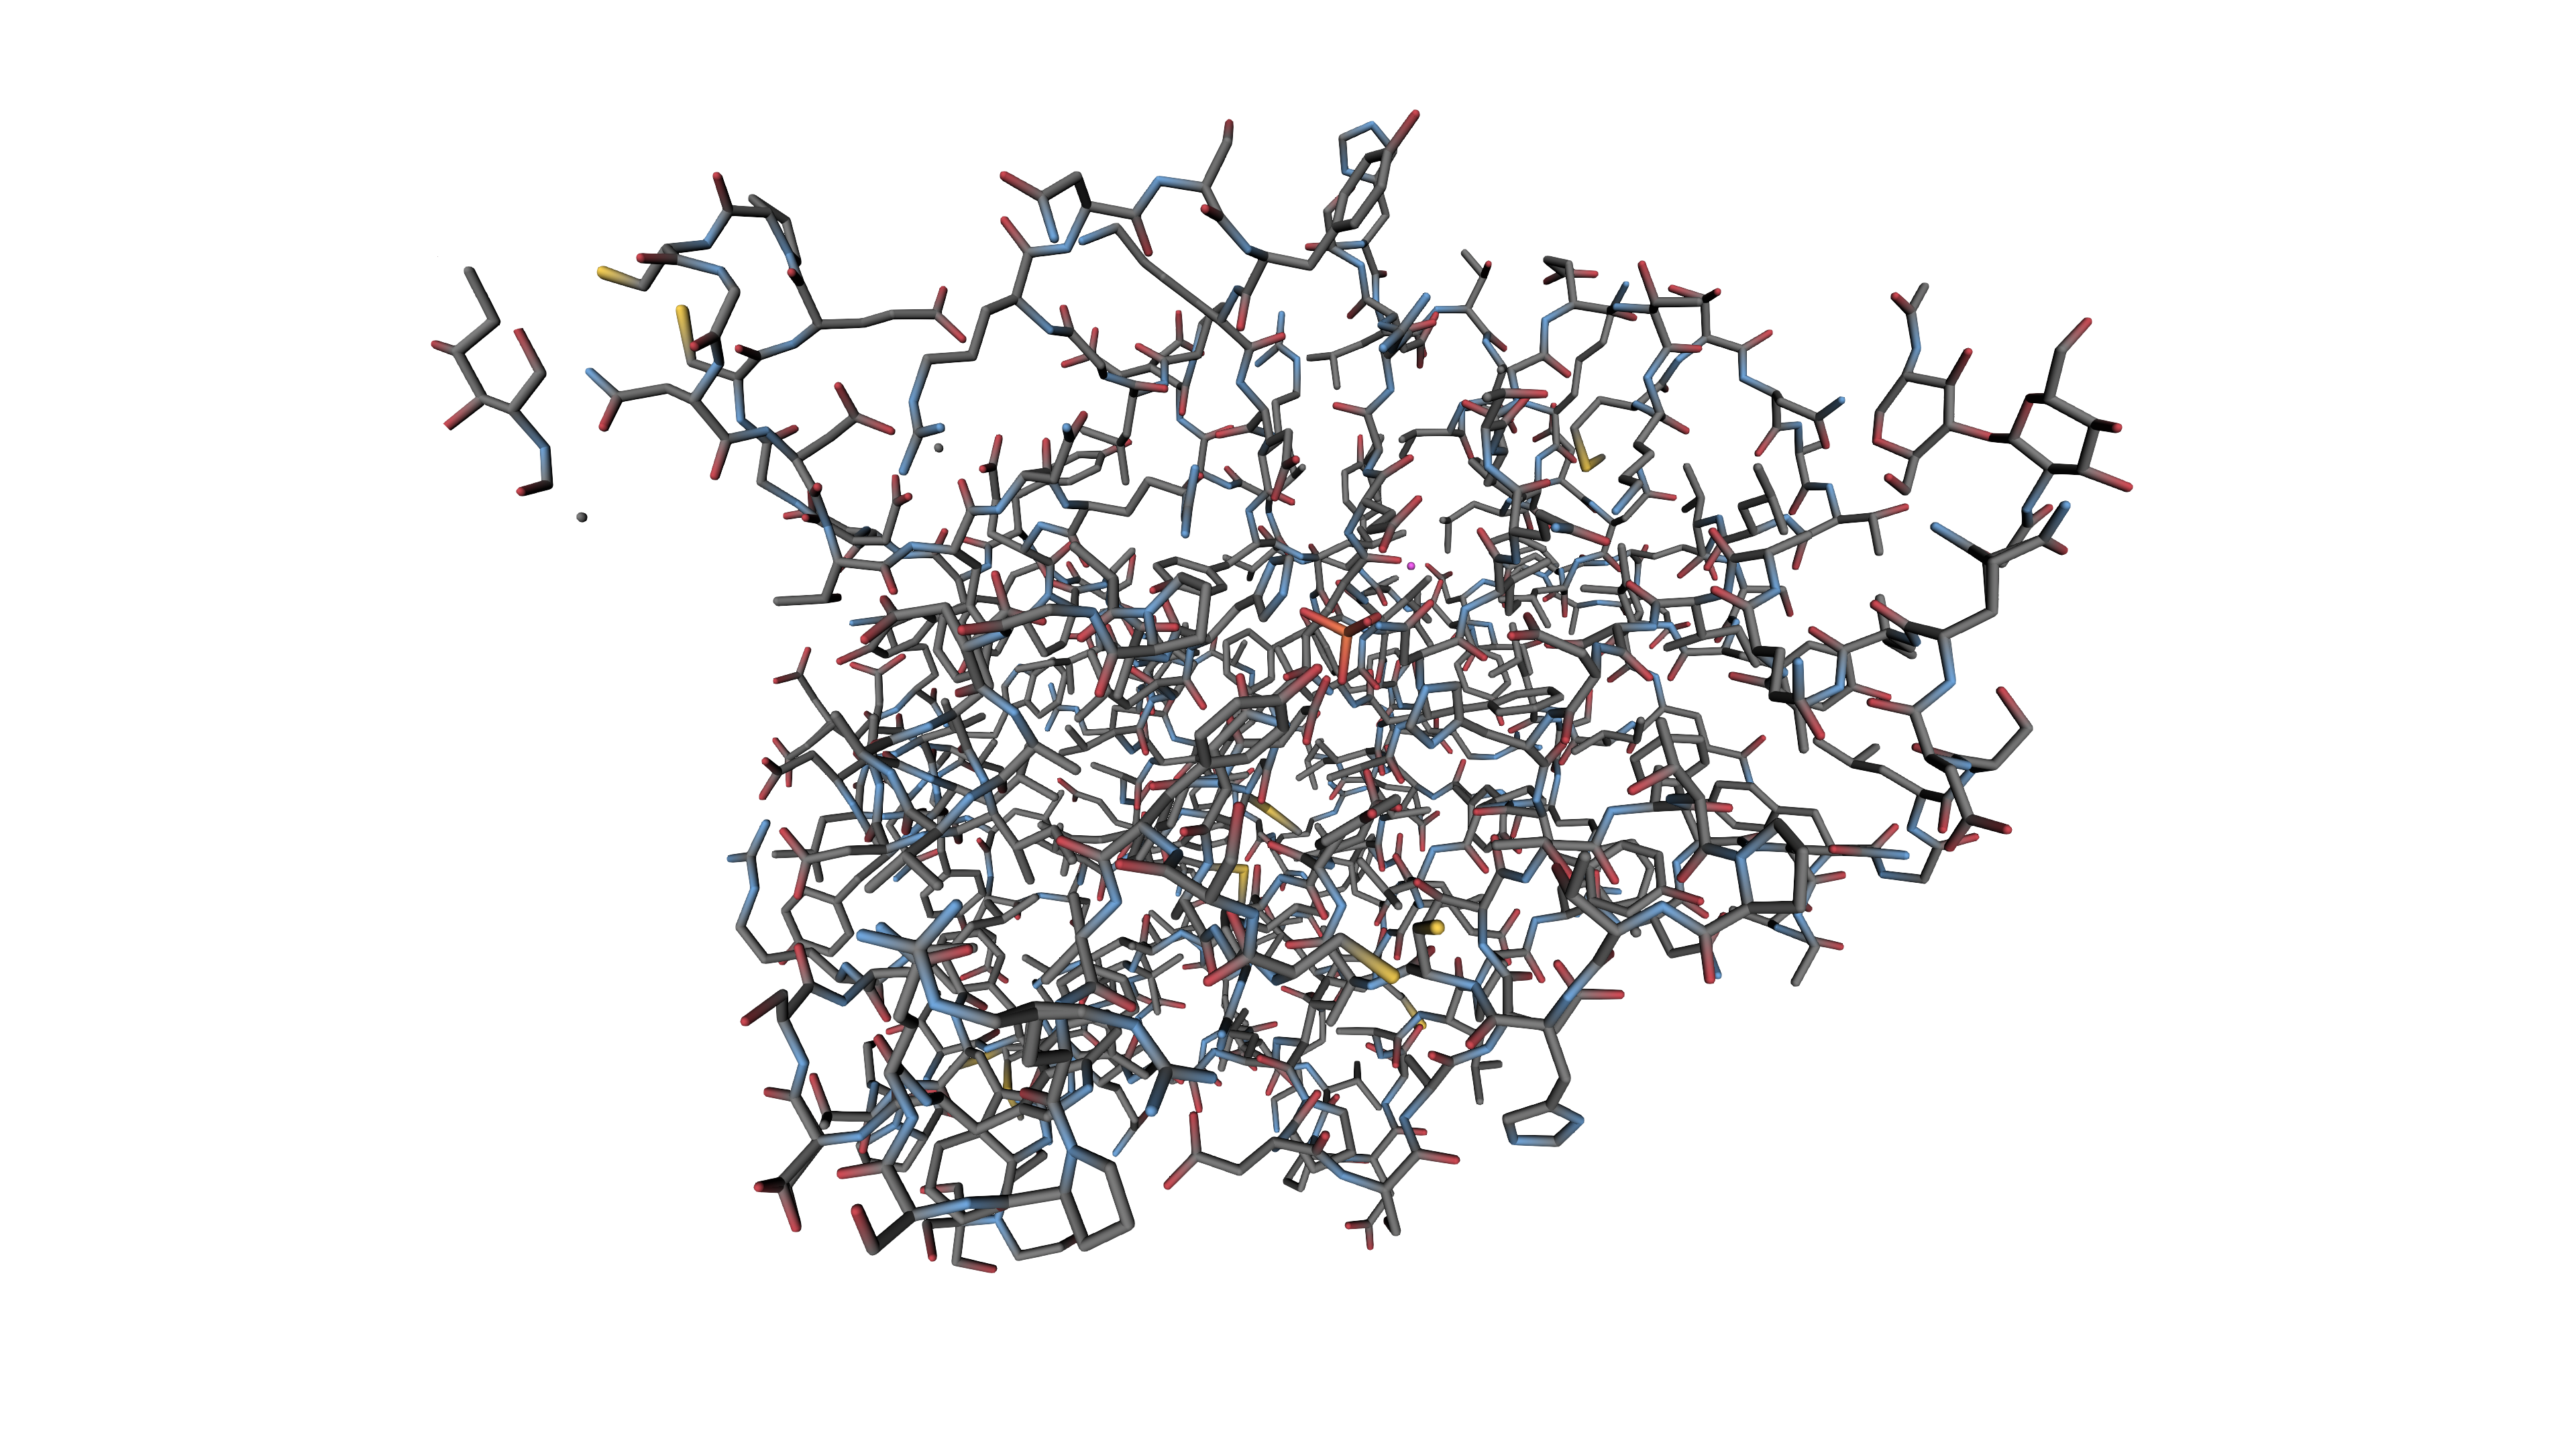
\includegraphics[width=\textwidth]{./figures/ch1/4awn_licorice}
			\caption{Représentation en \og bâtons \fg{} encore appelée en \og réglisse \fg{}, ou \emph{licorice} en anglais. Seules les liaisons covalentes sont visibles}
			\label{fig:4awn_licorice}
		\end{subfigure}
		~
		\begin{subfigure}[t]{\subImgW}
			\centering
			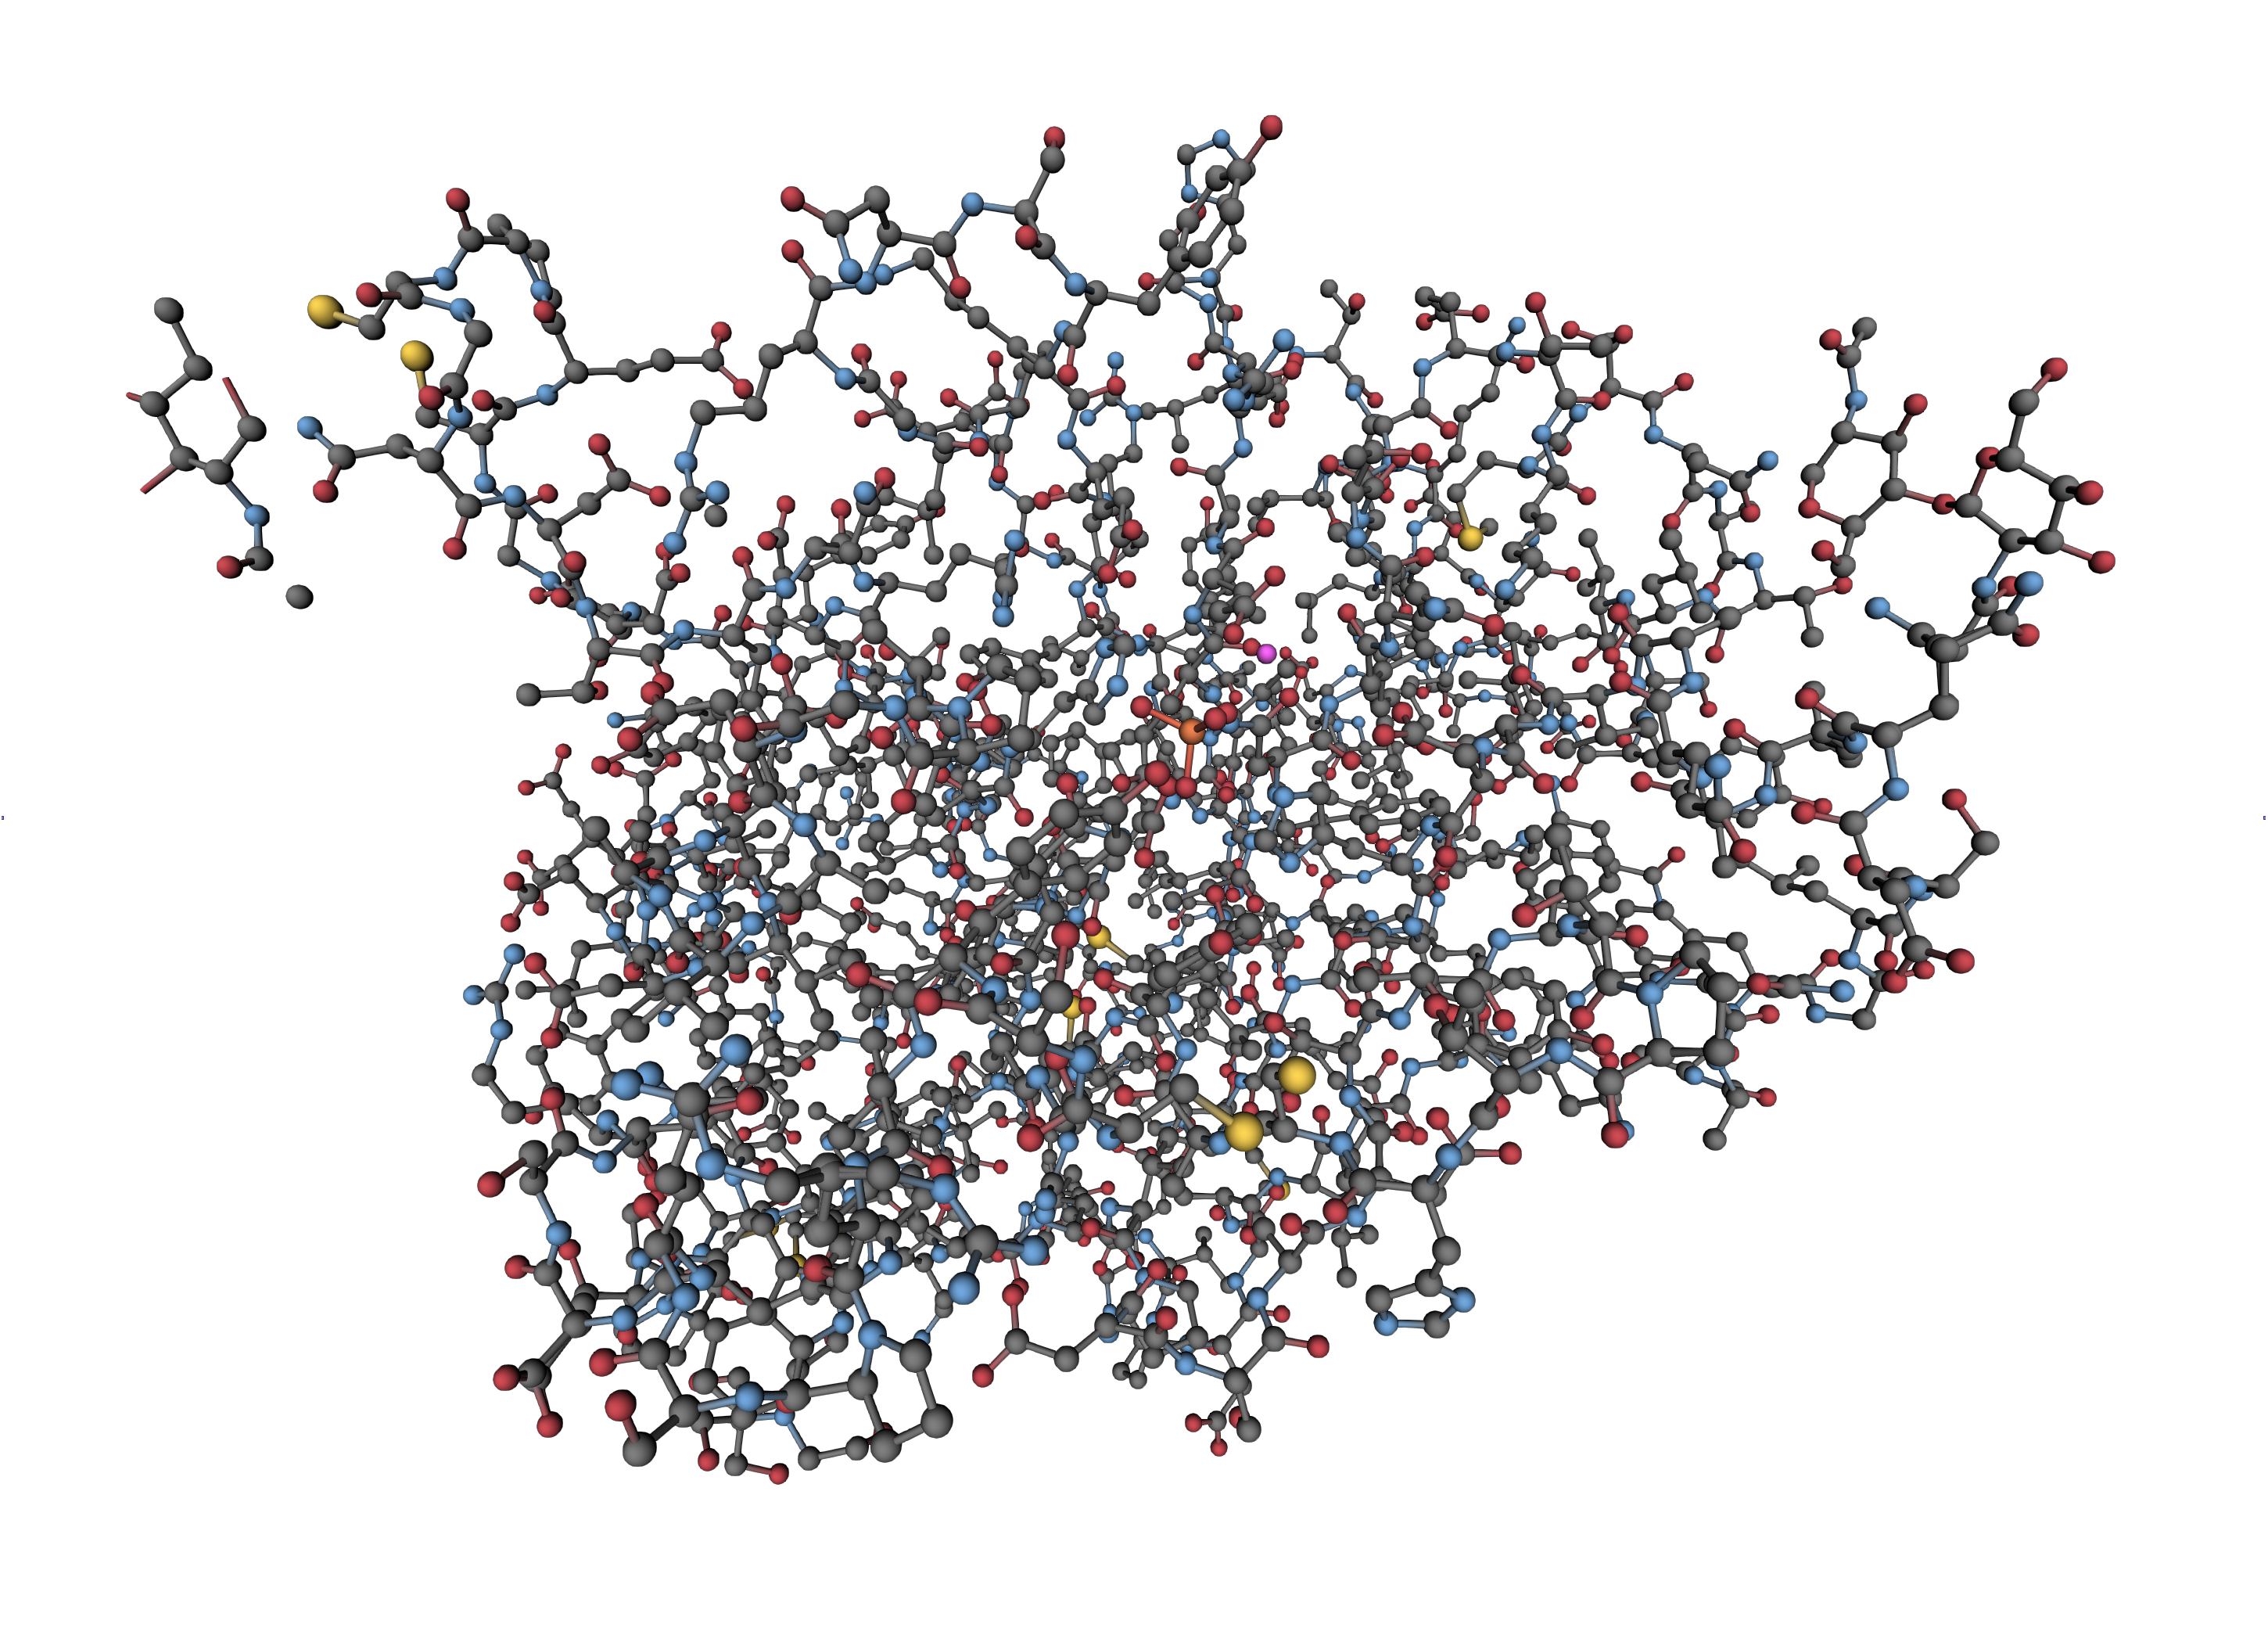
\includegraphics[width=\textwidth]{./figures/ch1/4awn_CPK}
			\caption{Représentation dite CPK, ou en \og boules et bâtons \fg{}. Les atomes et les liaisons sont représentés.}
			\label{fig:4awn_CPK}
		\end{subfigure}
		~
		\begin{subfigure}[t]{\subImgW}
			\centering
			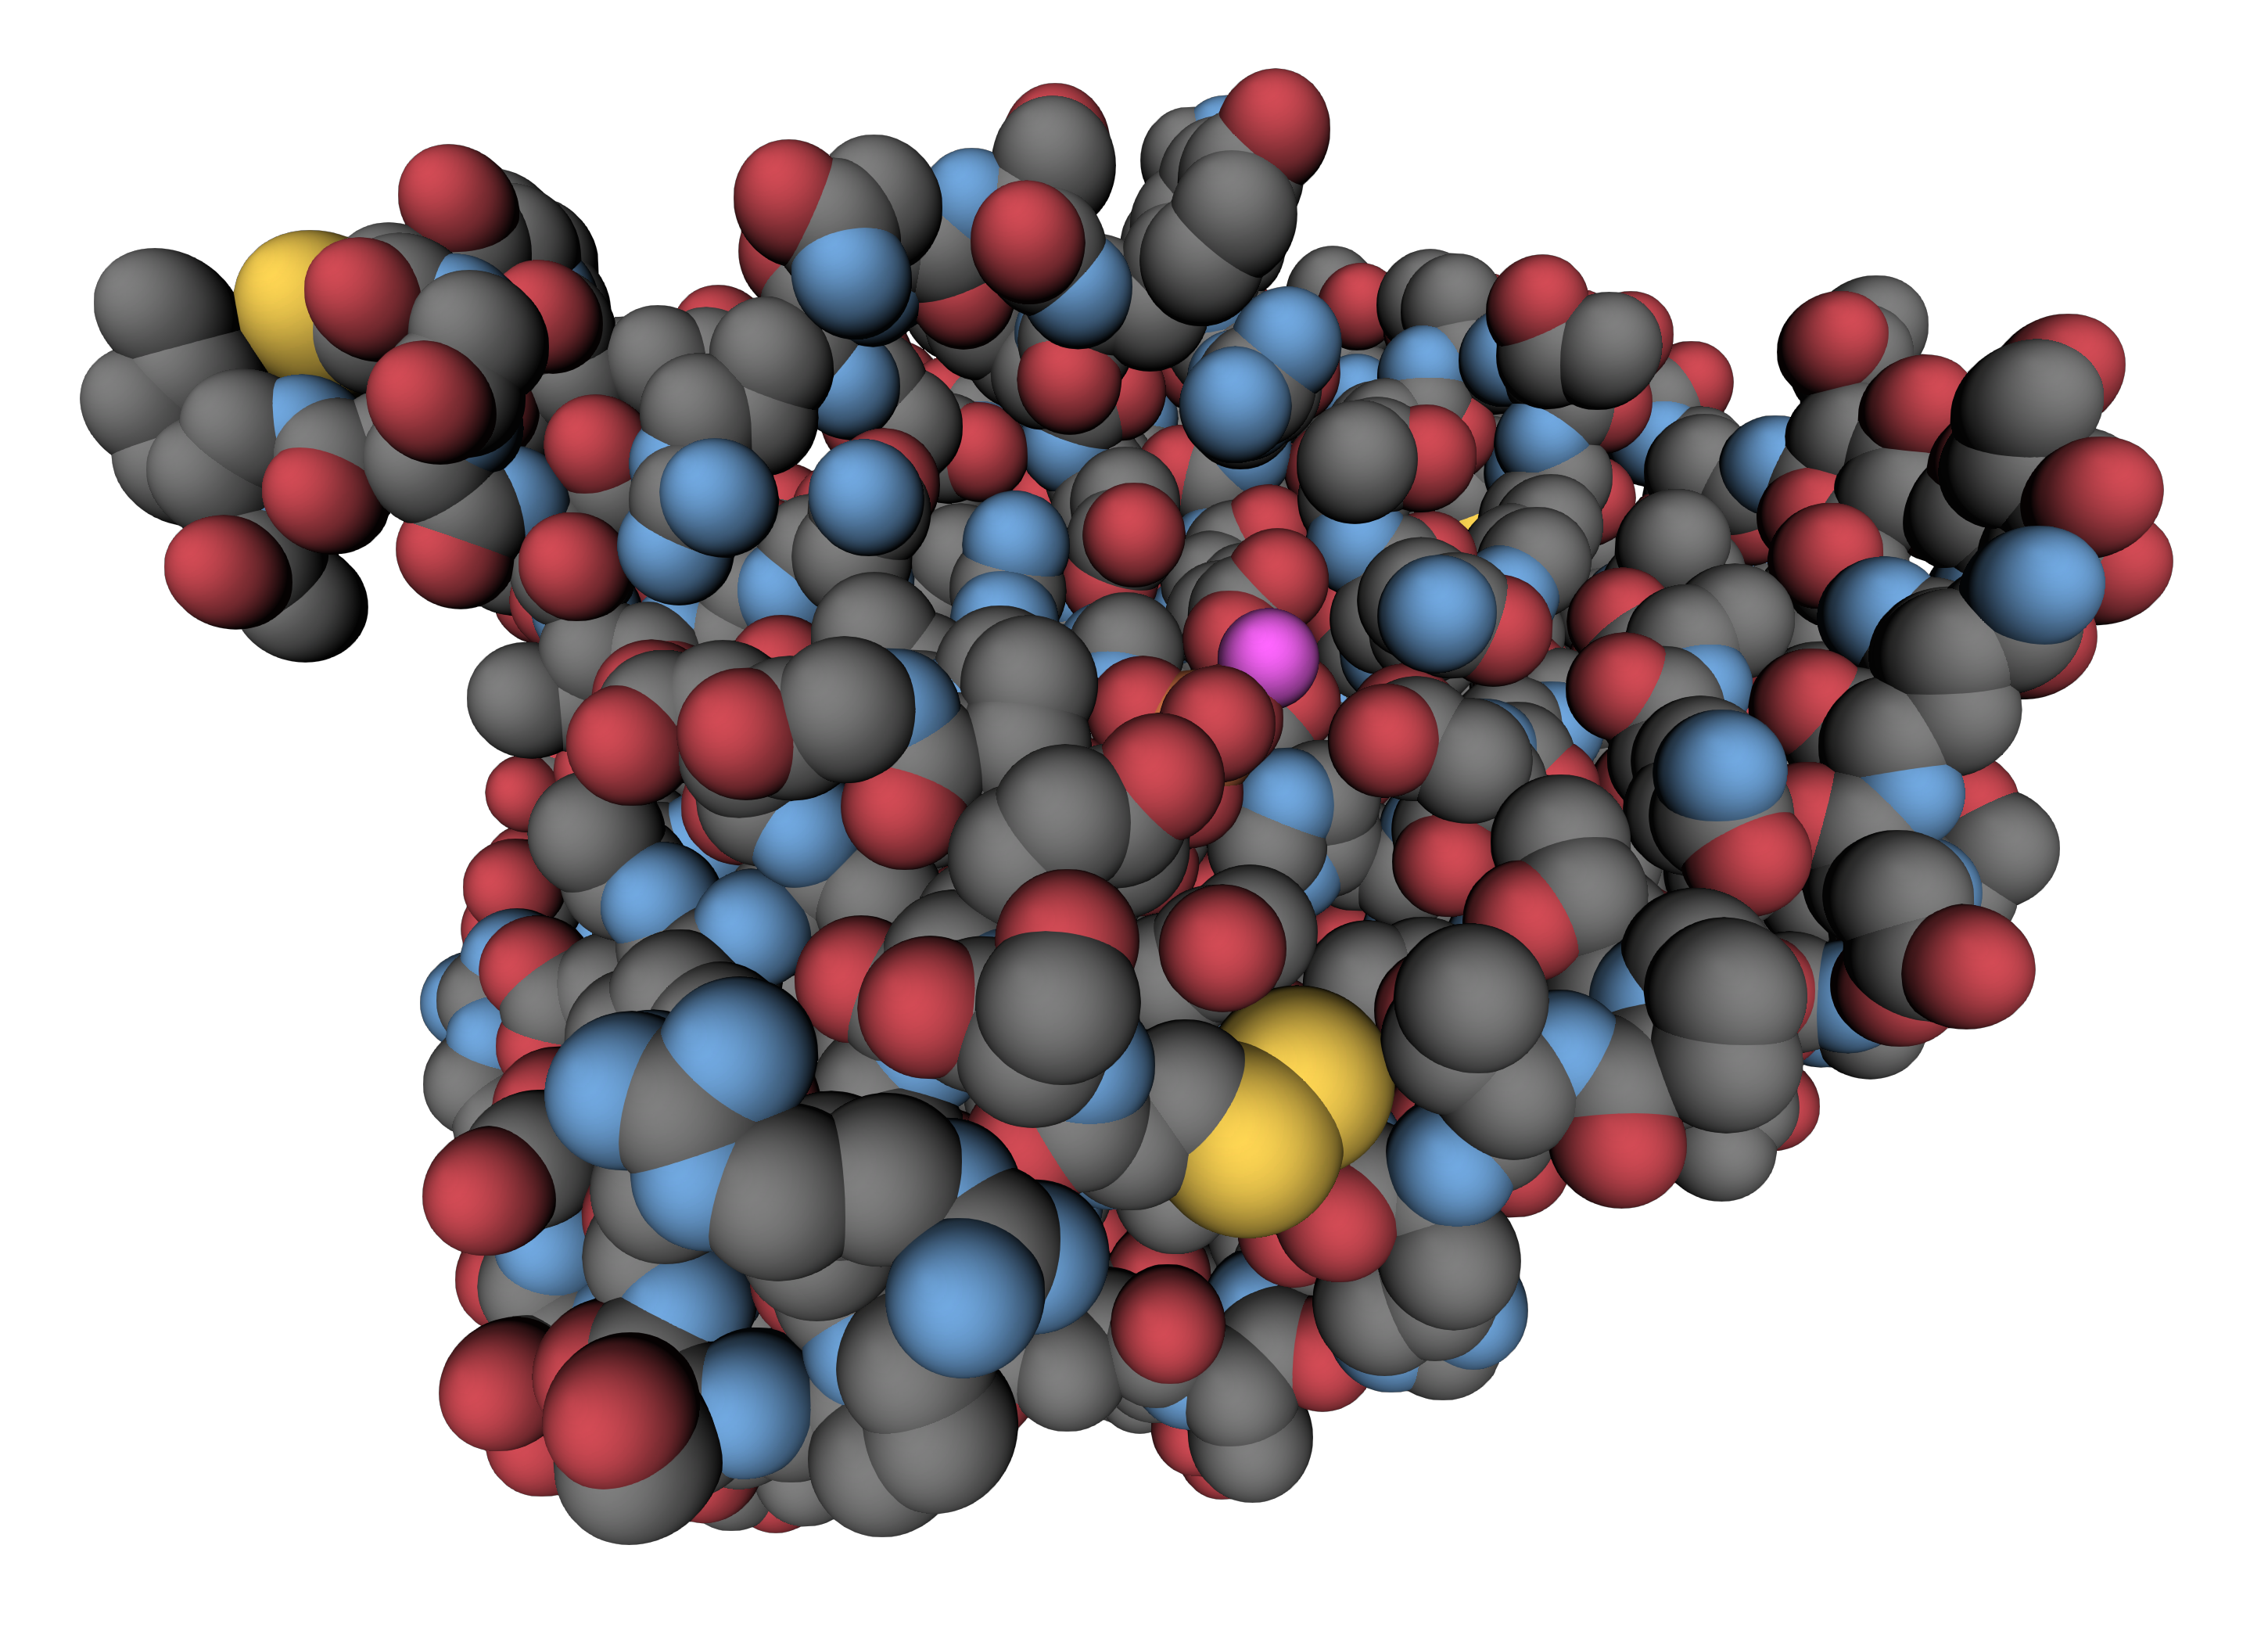
\includegraphics[width=\textwidth]{./figures/ch1/4awn_vdW}
			\caption{Représentation basée sur le rayon de van der Waals. Seuls les atomes sont visibles.}
			\label{fig:4awn_VdW}
		\end{subfigure}
		~
		\begin{subfigure}[t]{\subImgW}
			\centering
			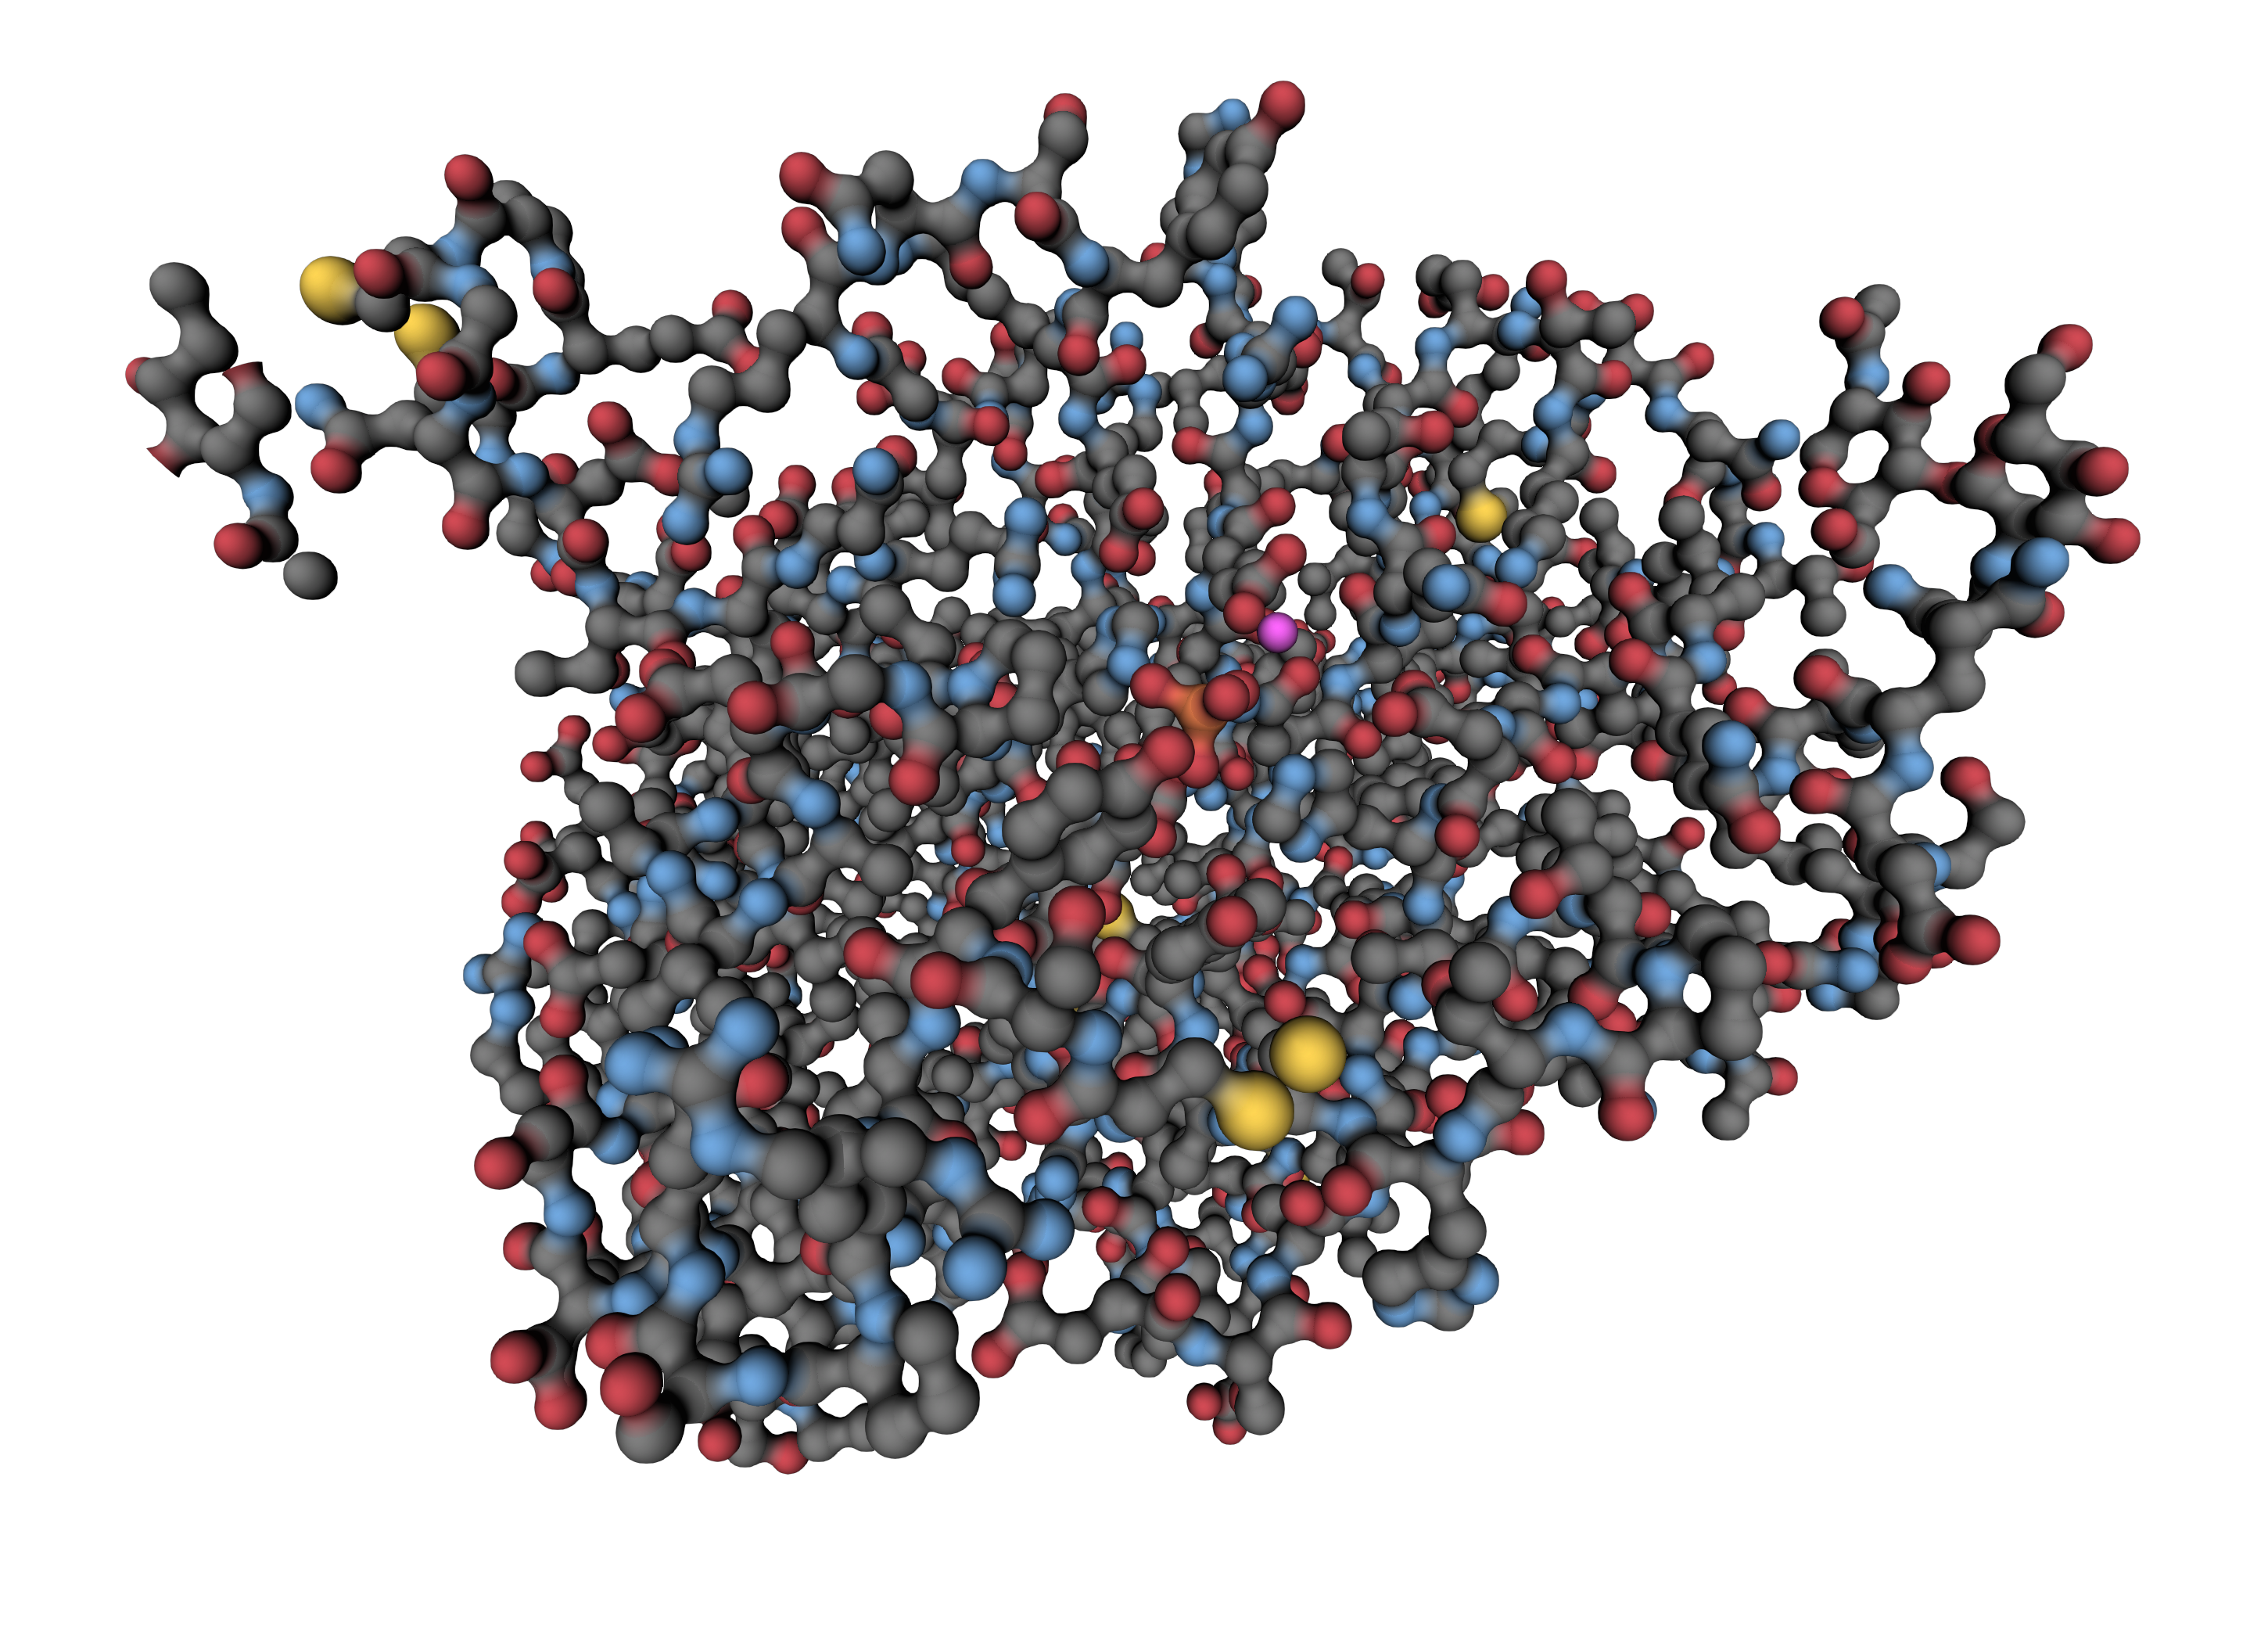
\includegraphics[width=\textwidth]{./figures/ch1/4awn_HB}
			\caption{Représentation en \emph{Hyperballs}~\cite{chavent2011gpu}. Les atomes et les liaisons sont représentés.}
			\label{fig:4awn_HB}
		\end{subfigure}
		~
		\begin{subfigure}[t]{\subImgW}
			\centering
			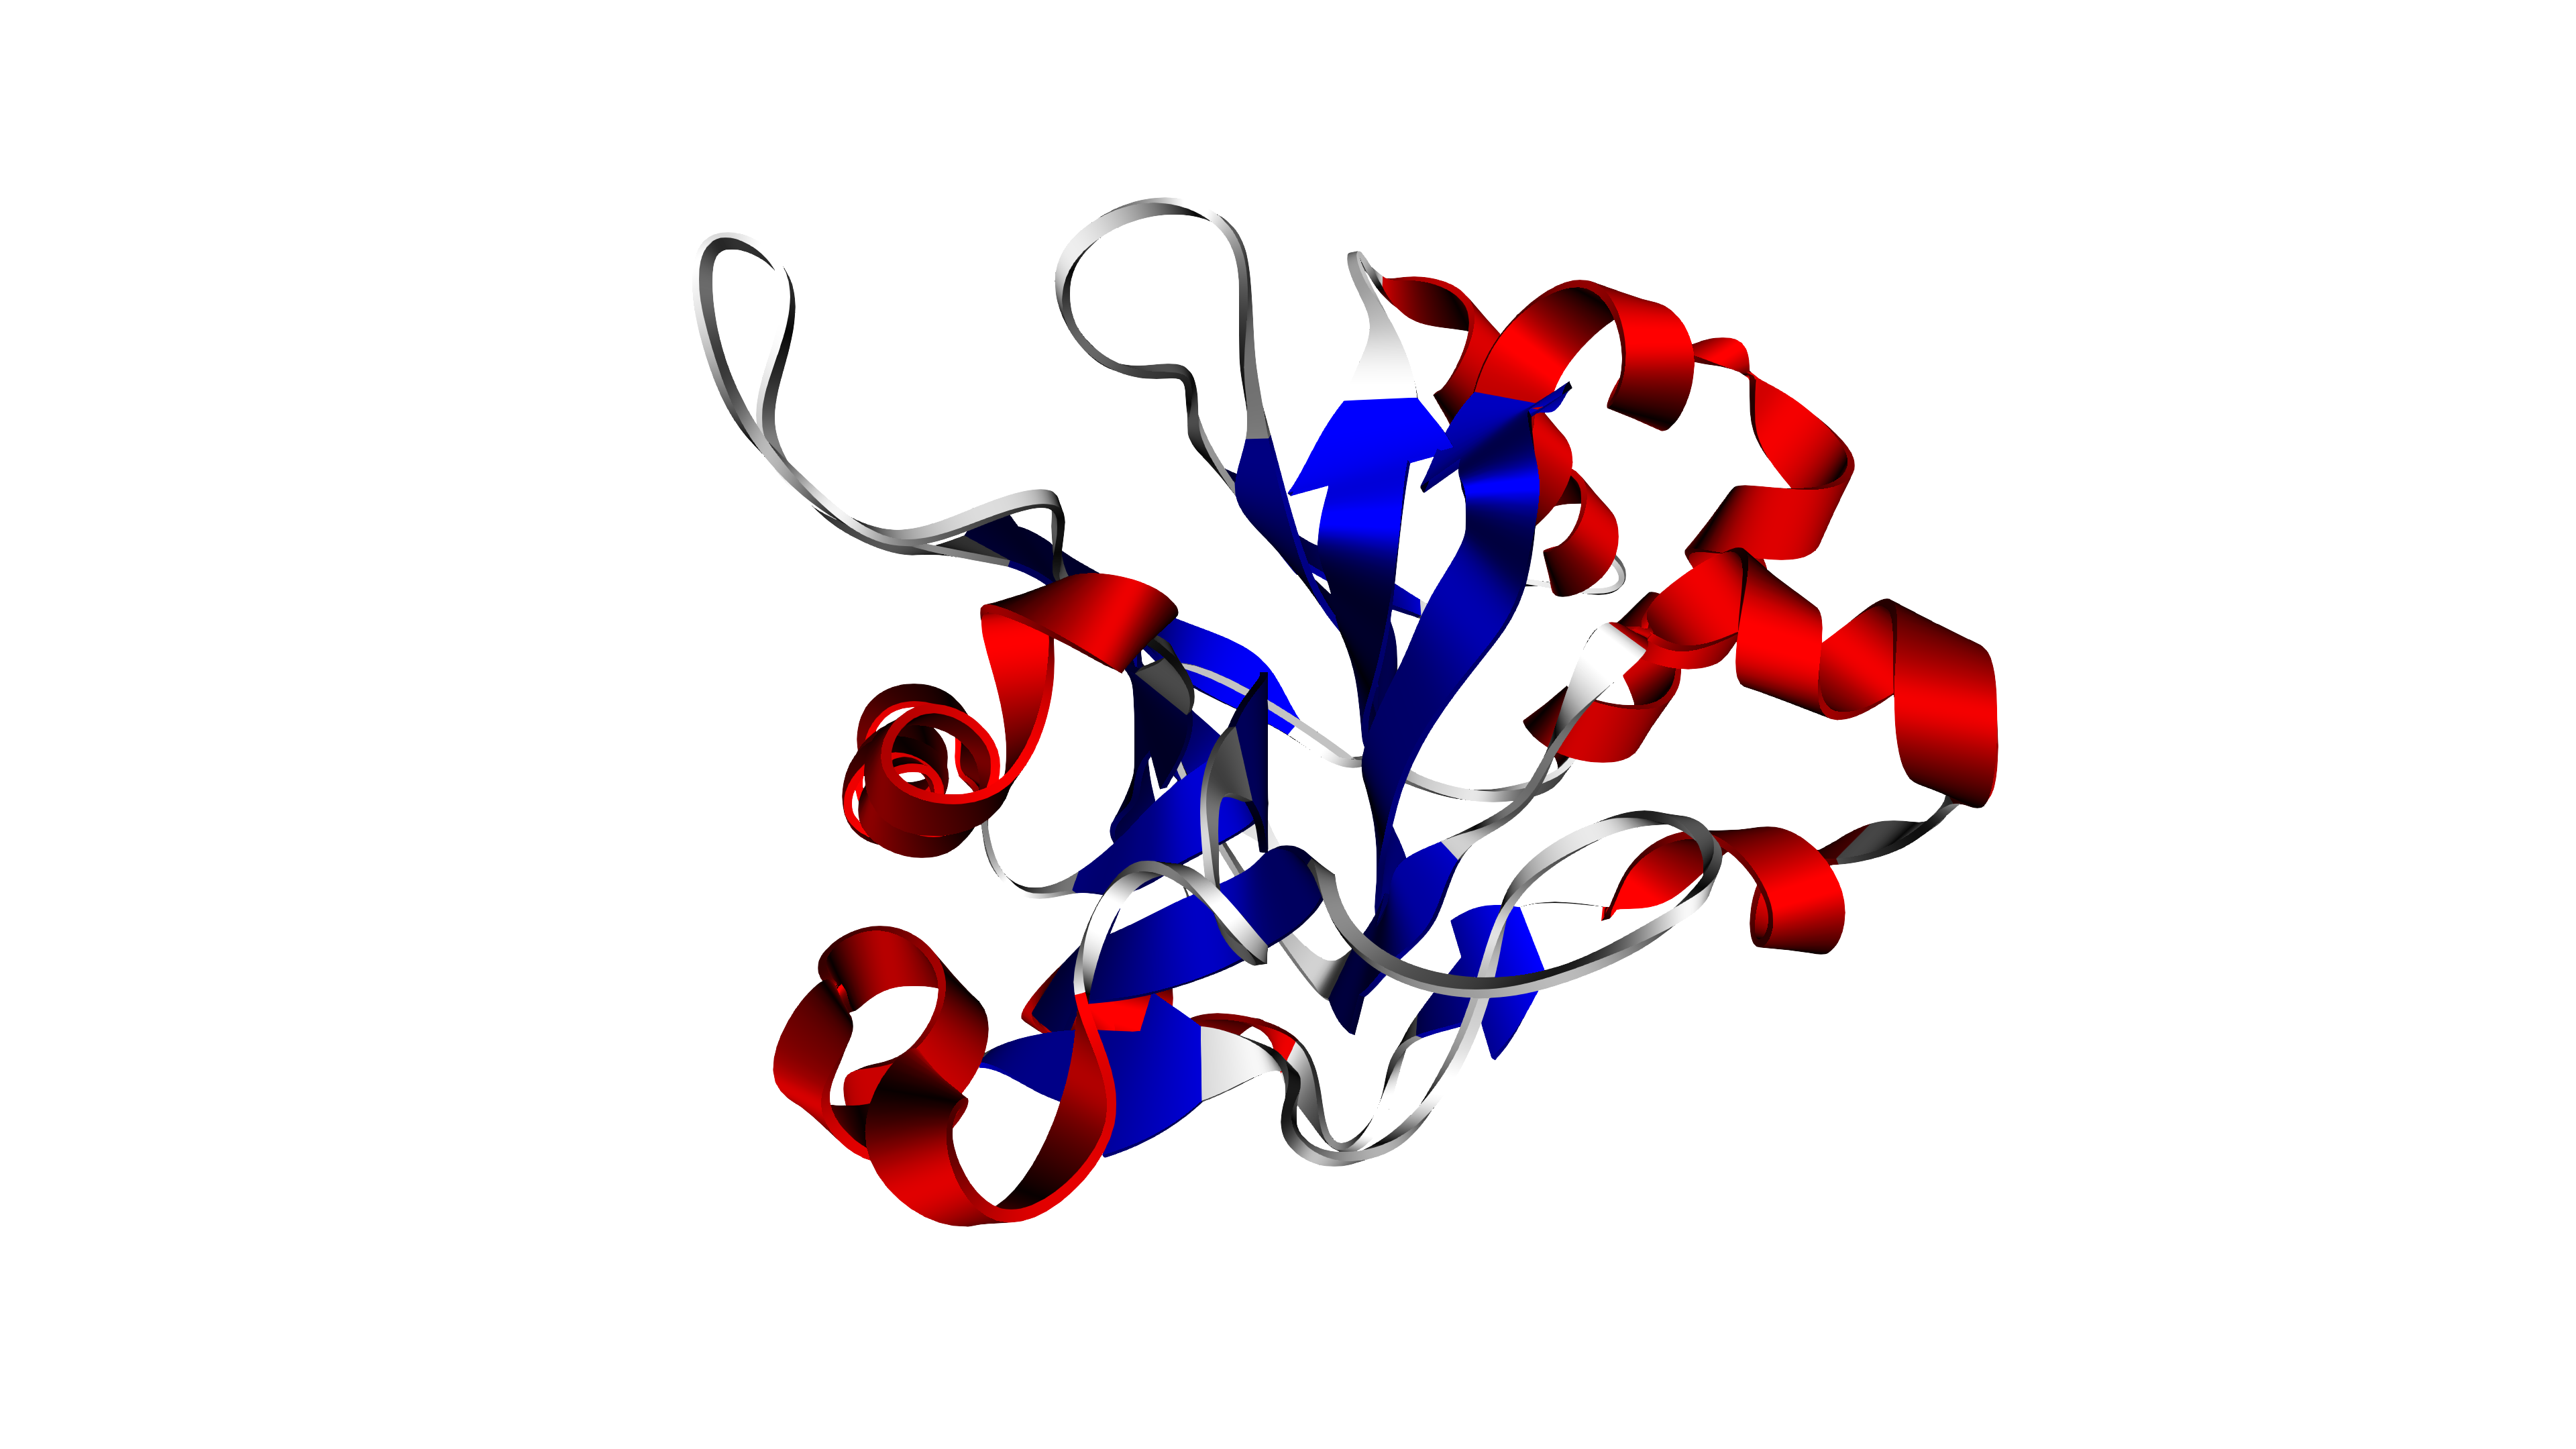
\includegraphics[width=\textwidth]{./figures/ch1/4awn_ss}
			\caption{Représentation en structures secondaires. Les atomes et les liaisons sont invisibles, mais des structures plus grandes sont représentées de façon schématique.}
			\label{fig:4awn_ss}
		\end{subfigure}
		\caption{La désoxyribonucléase (ou ADNase) est une enzyme catalysant les acides désoxyribonucléiques en nucléotides ou polynucléotides. Elle hydrolyse les liaisons phosphodiester. Voici un échantillon de quelques techniques de visualisation moléculaire, avec l'ADNase pour objet. Illustrations produites par \emph{UnityMol}~\cite{doutreligne2014unitymol} à partir d'une structure de la \emph{Protein Data Bank}~\cite{parsiegla2012structure}.}
		\label{fig:4awn_atom}
	\end{figure}
	
	\begin{figure}[H]
		\begin{subfigure}[t]{\subImgW}
			\centering
			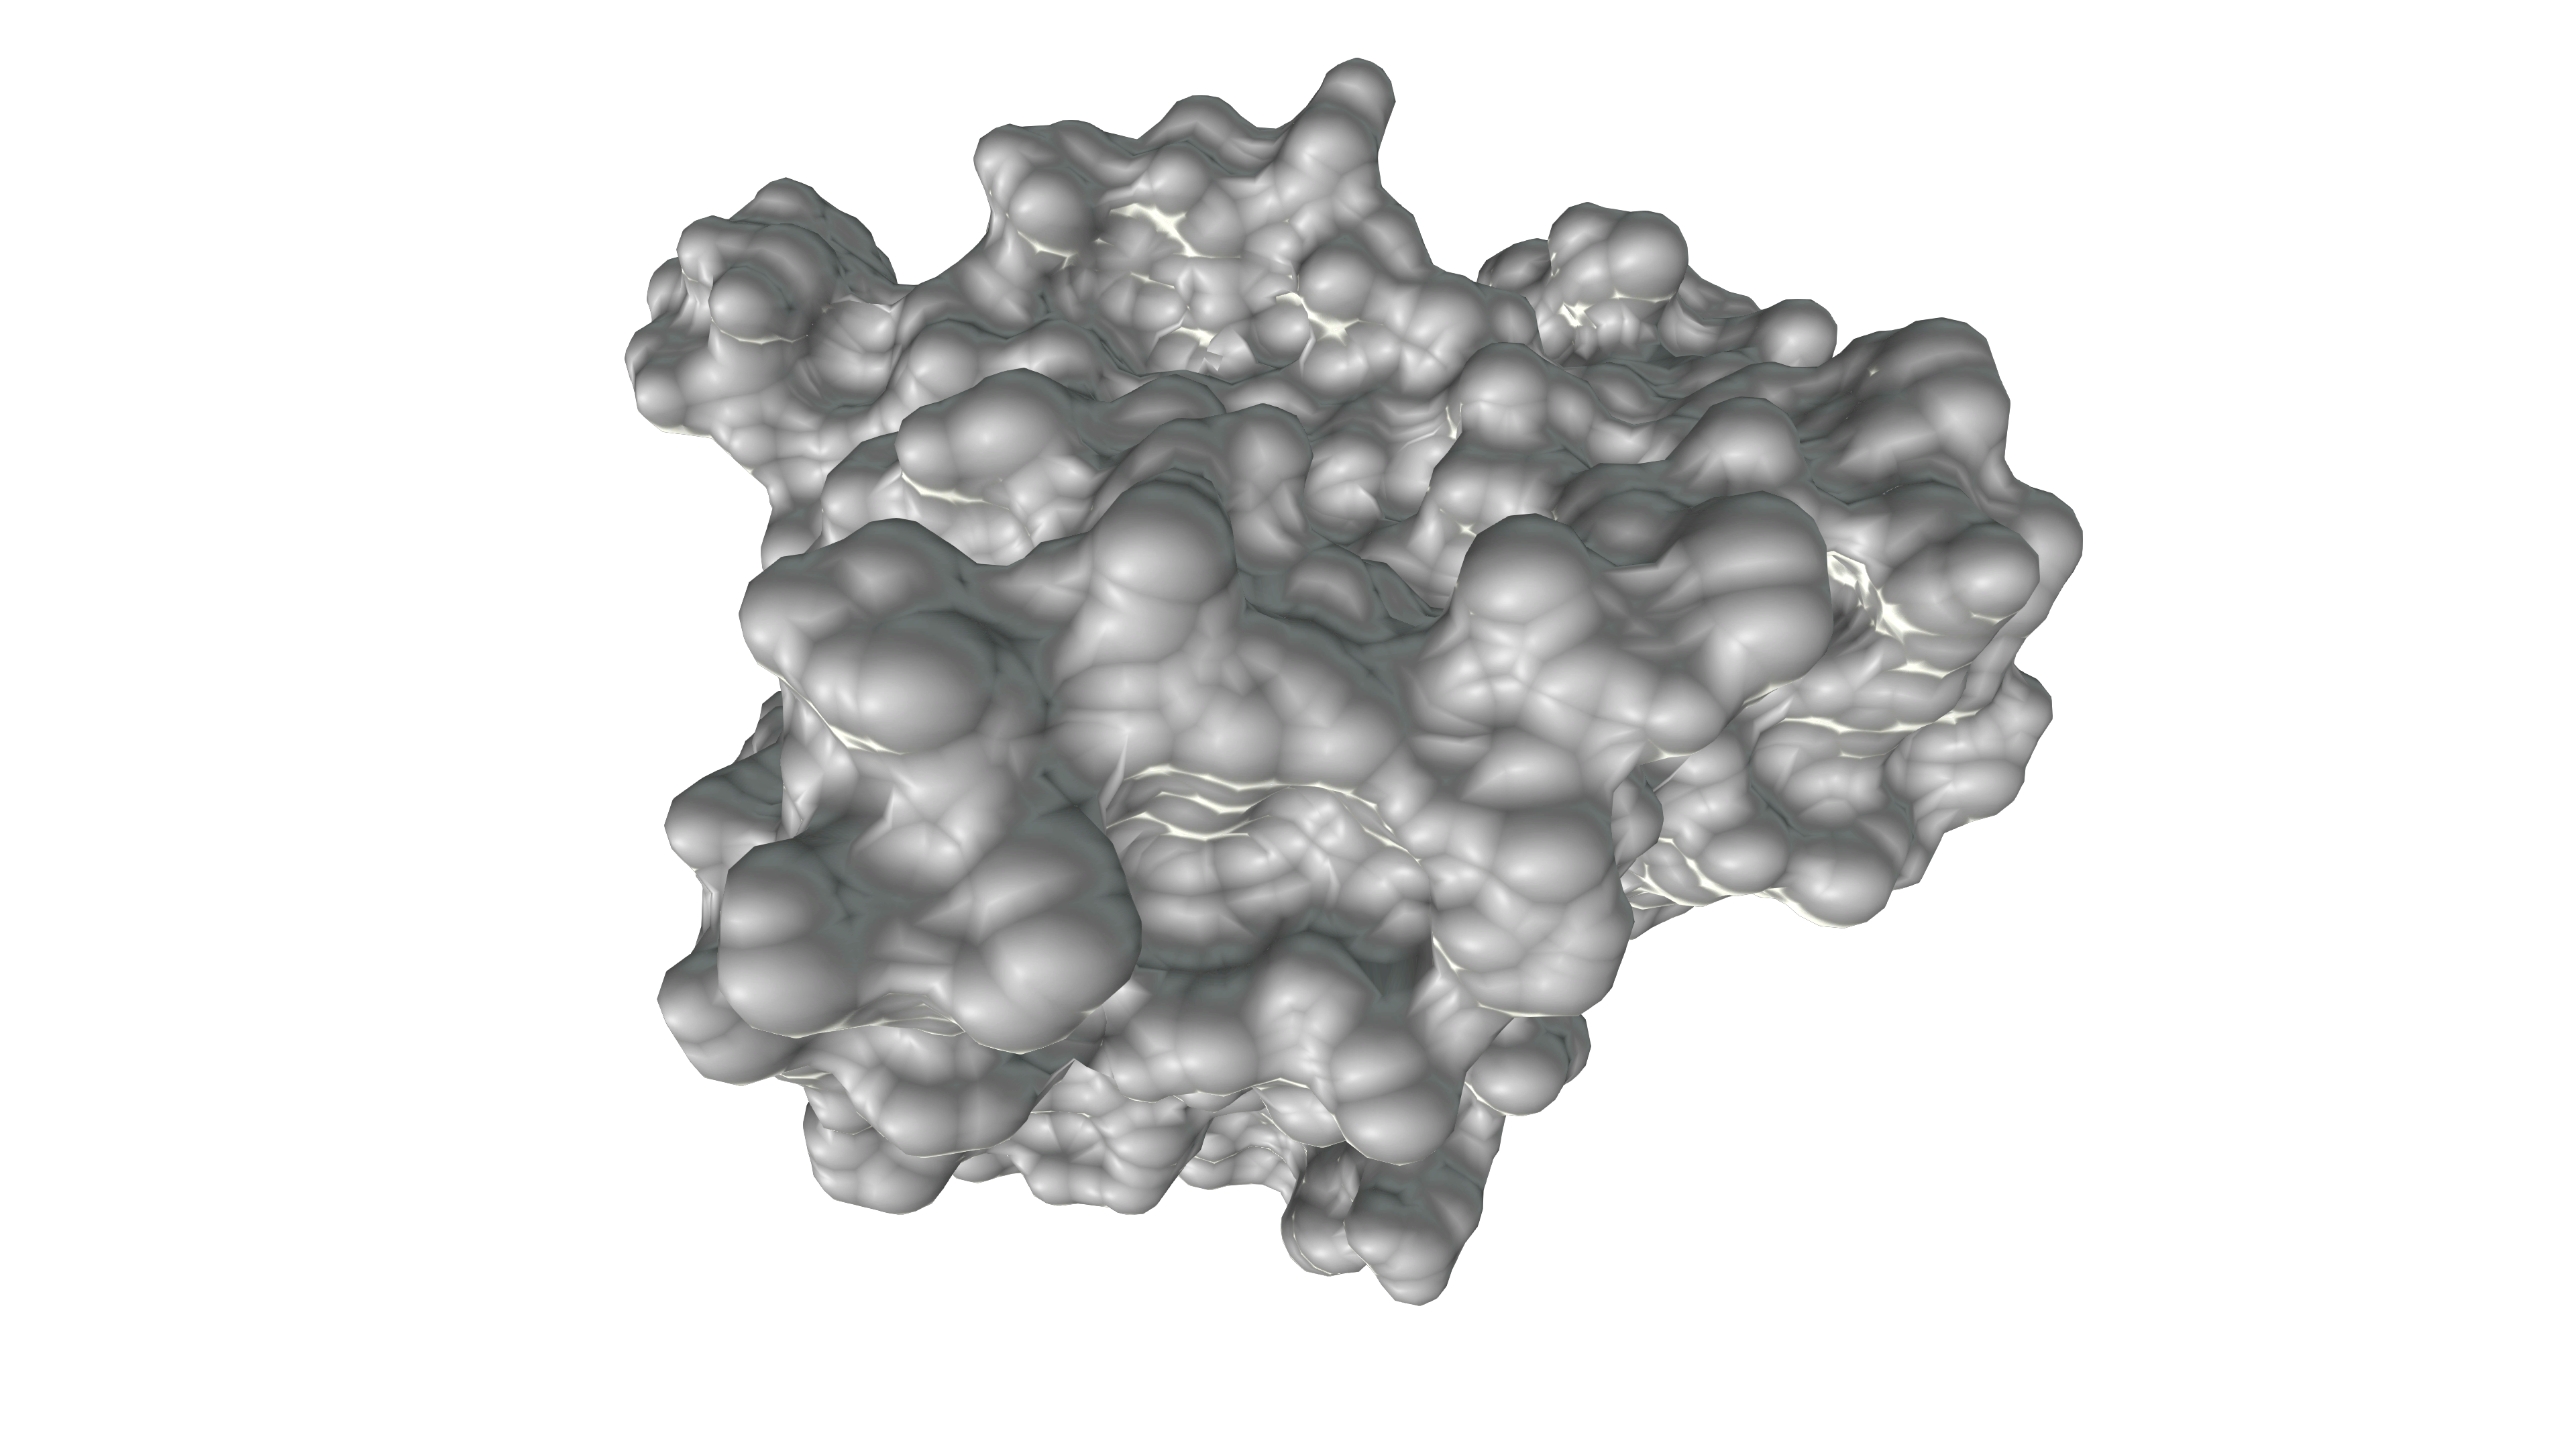
\includegraphics[width=\textwidth]{./figures/ch1/4awn_sas}
			\caption{Surface accessible au solvant, correspondant aux points parcourus par le centre d'une molécule d'eau en contact avec l'ADNase.}
			\label{fig:4awn_sas}
		\end{subfigure}
		~
		\begin{subfigure}[t]{\subImgW}
			\centering
			\includegraphics[width=\textwidth]{./figures/ch1/4awn_ses}
			\caption{Surface de Connolly, ou \emph{solvent excluded surface}, correspondant aux points de contact entre une molécule d'eau et l'ADNase.}
			\label{fig:4awn_ses}
		\end{subfigure}
		~
		\begin{subfigure}[t]{\subImgW}
			\centering
			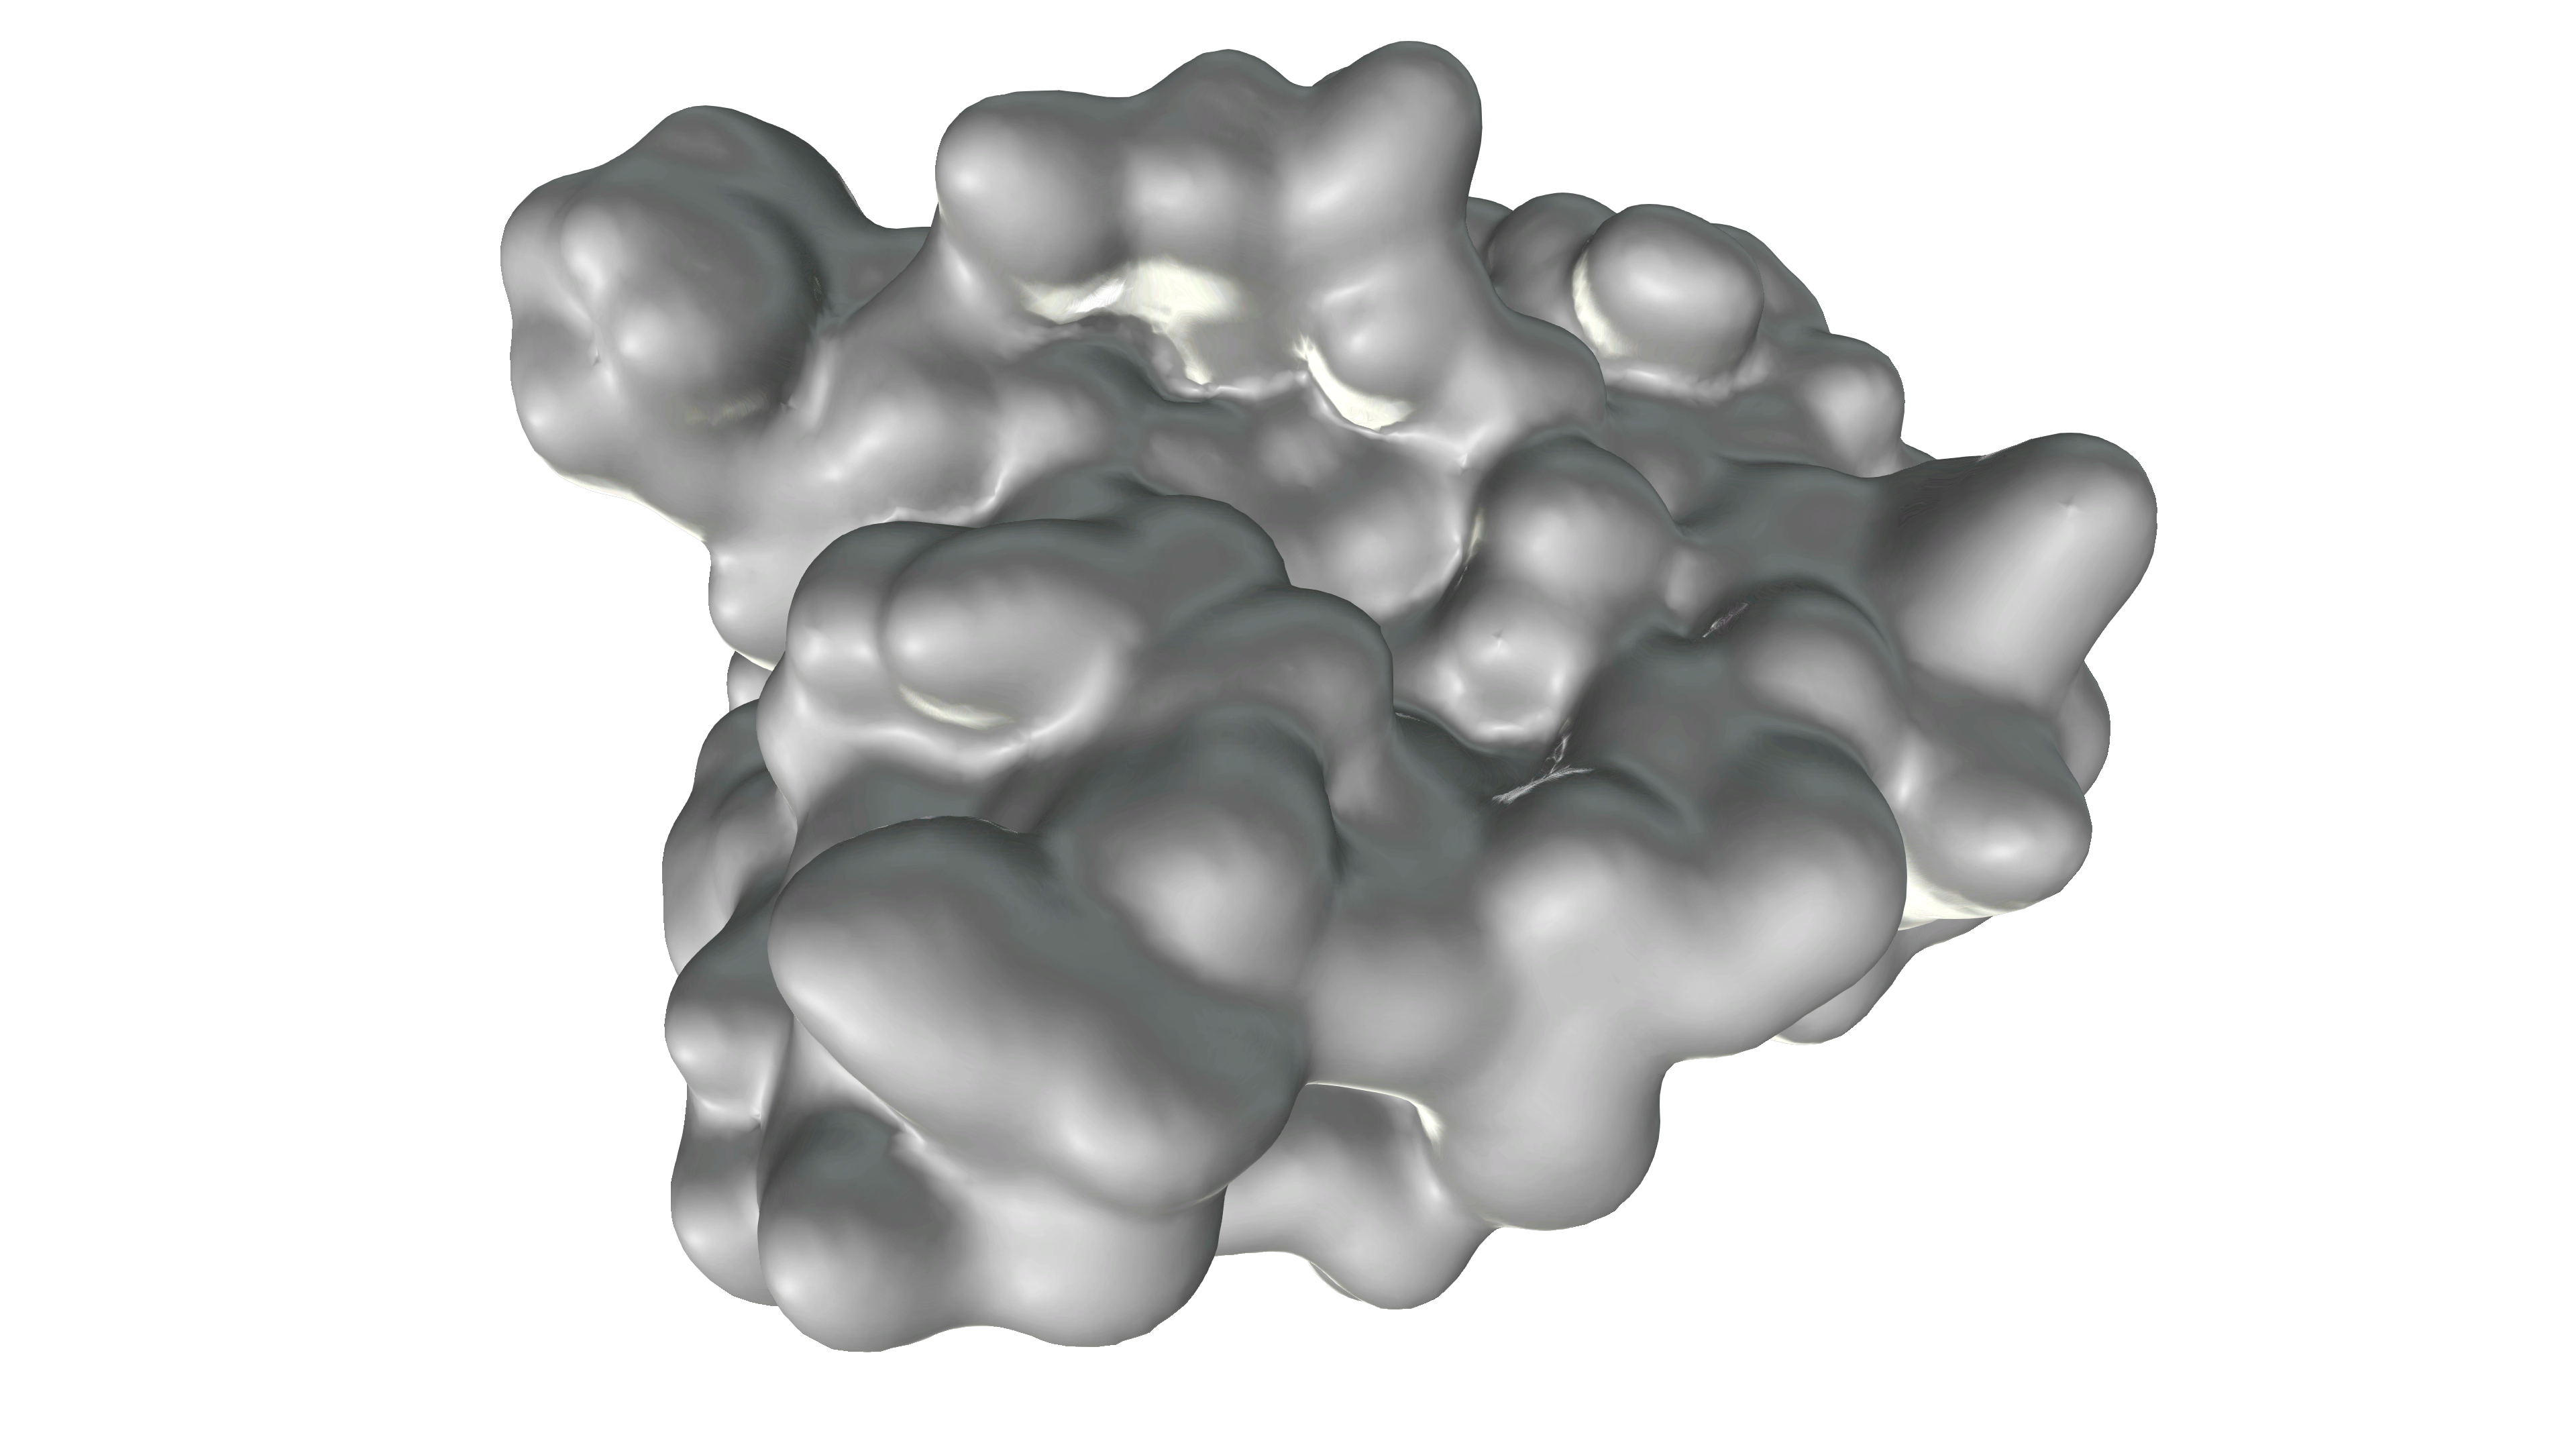
\includegraphics[width=\textwidth]{./figures/ch1/4awn_iso_0_2}
			\caption{Isosurface de densité, avec un seuil très faible, de $0,2$.}
			\label{fig:4awn_iso_0_2}
		\end{subfigure}
		~
		\begin{subfigure}[t]{\subImgW}
			\centering
			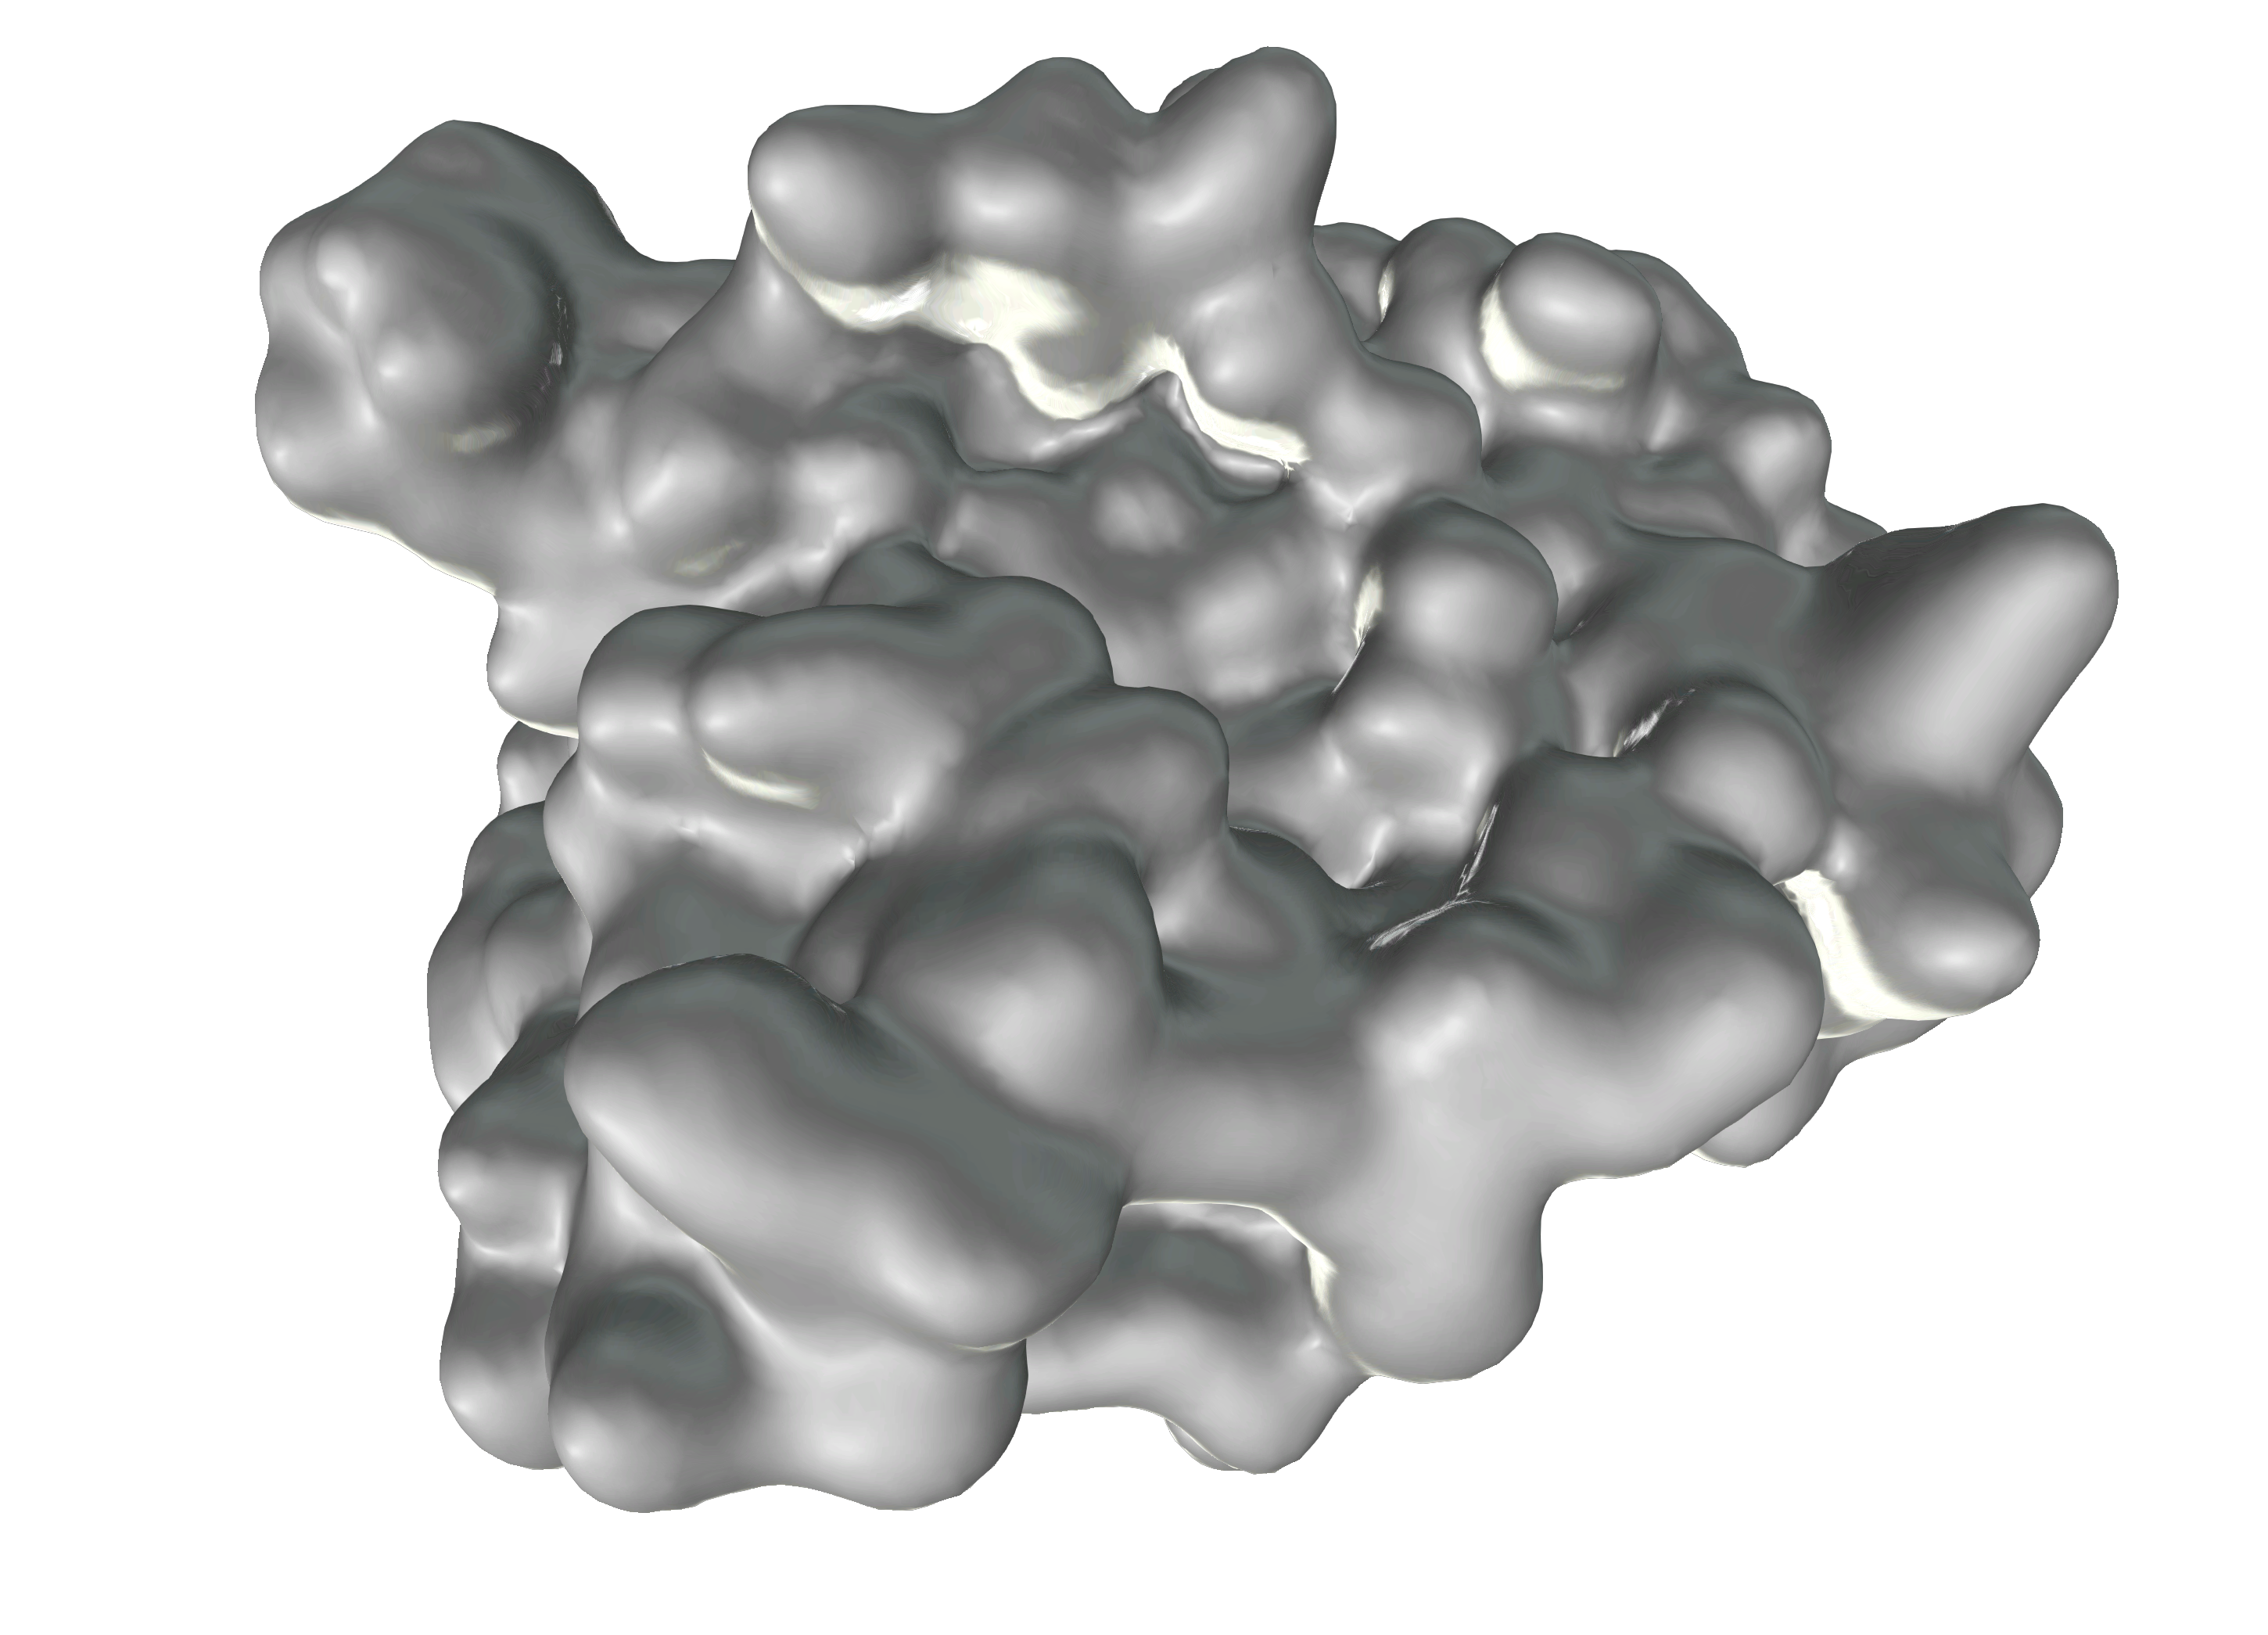
\includegraphics[width=\textwidth]{./figures/ch1/4awn_iso_0_5}
			\caption{Isosurface de densité, avec un seuil faible, de $0,5$.}
			\label{fig:4awn_iso_0_5}
		\end{subfigure}
		~
		\begin{subfigure}[t]{\subImgW}
			\centering
			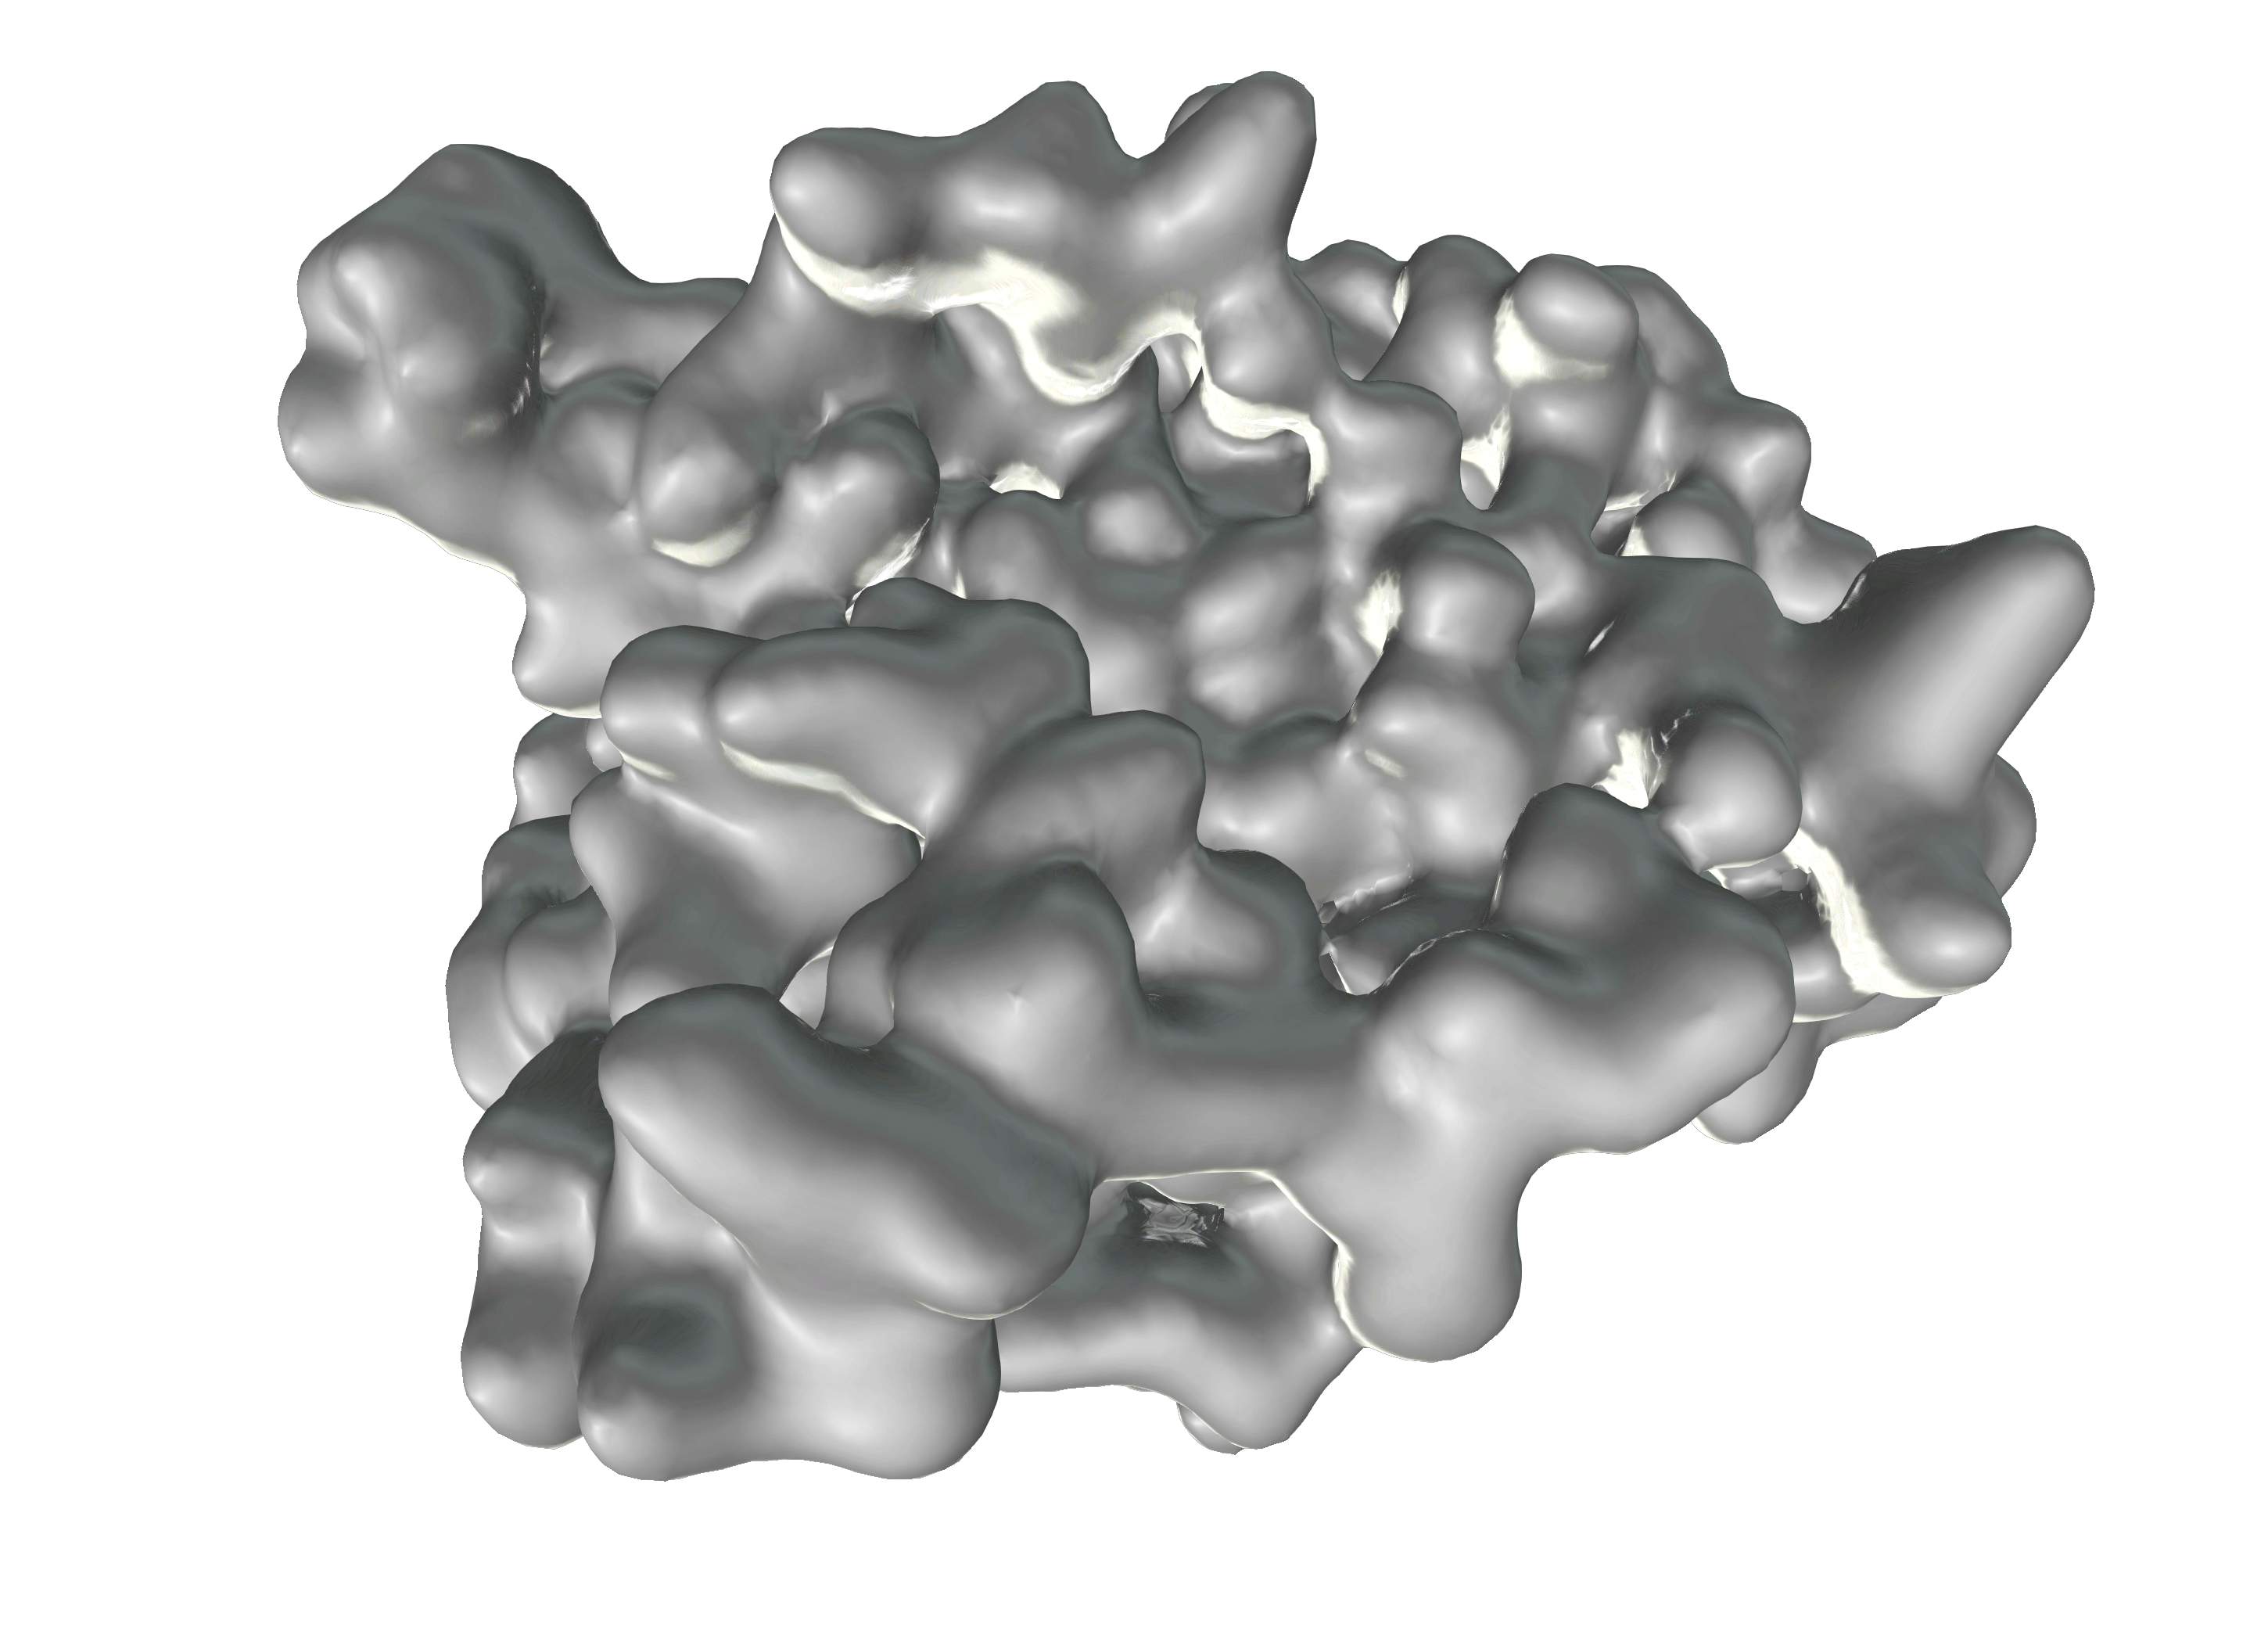
\includegraphics[width=\textwidth]{./figures/ch1/4awn_iso_1_0}
			\caption{Isosurface de densité, avec un seuil intermédiaire, de $1,0$.}
			\label{fig:4awn_iso_1_0}
		\end{subfigure}
		~
		\begin{subfigure}[t]{\subImgW}
			\centering
			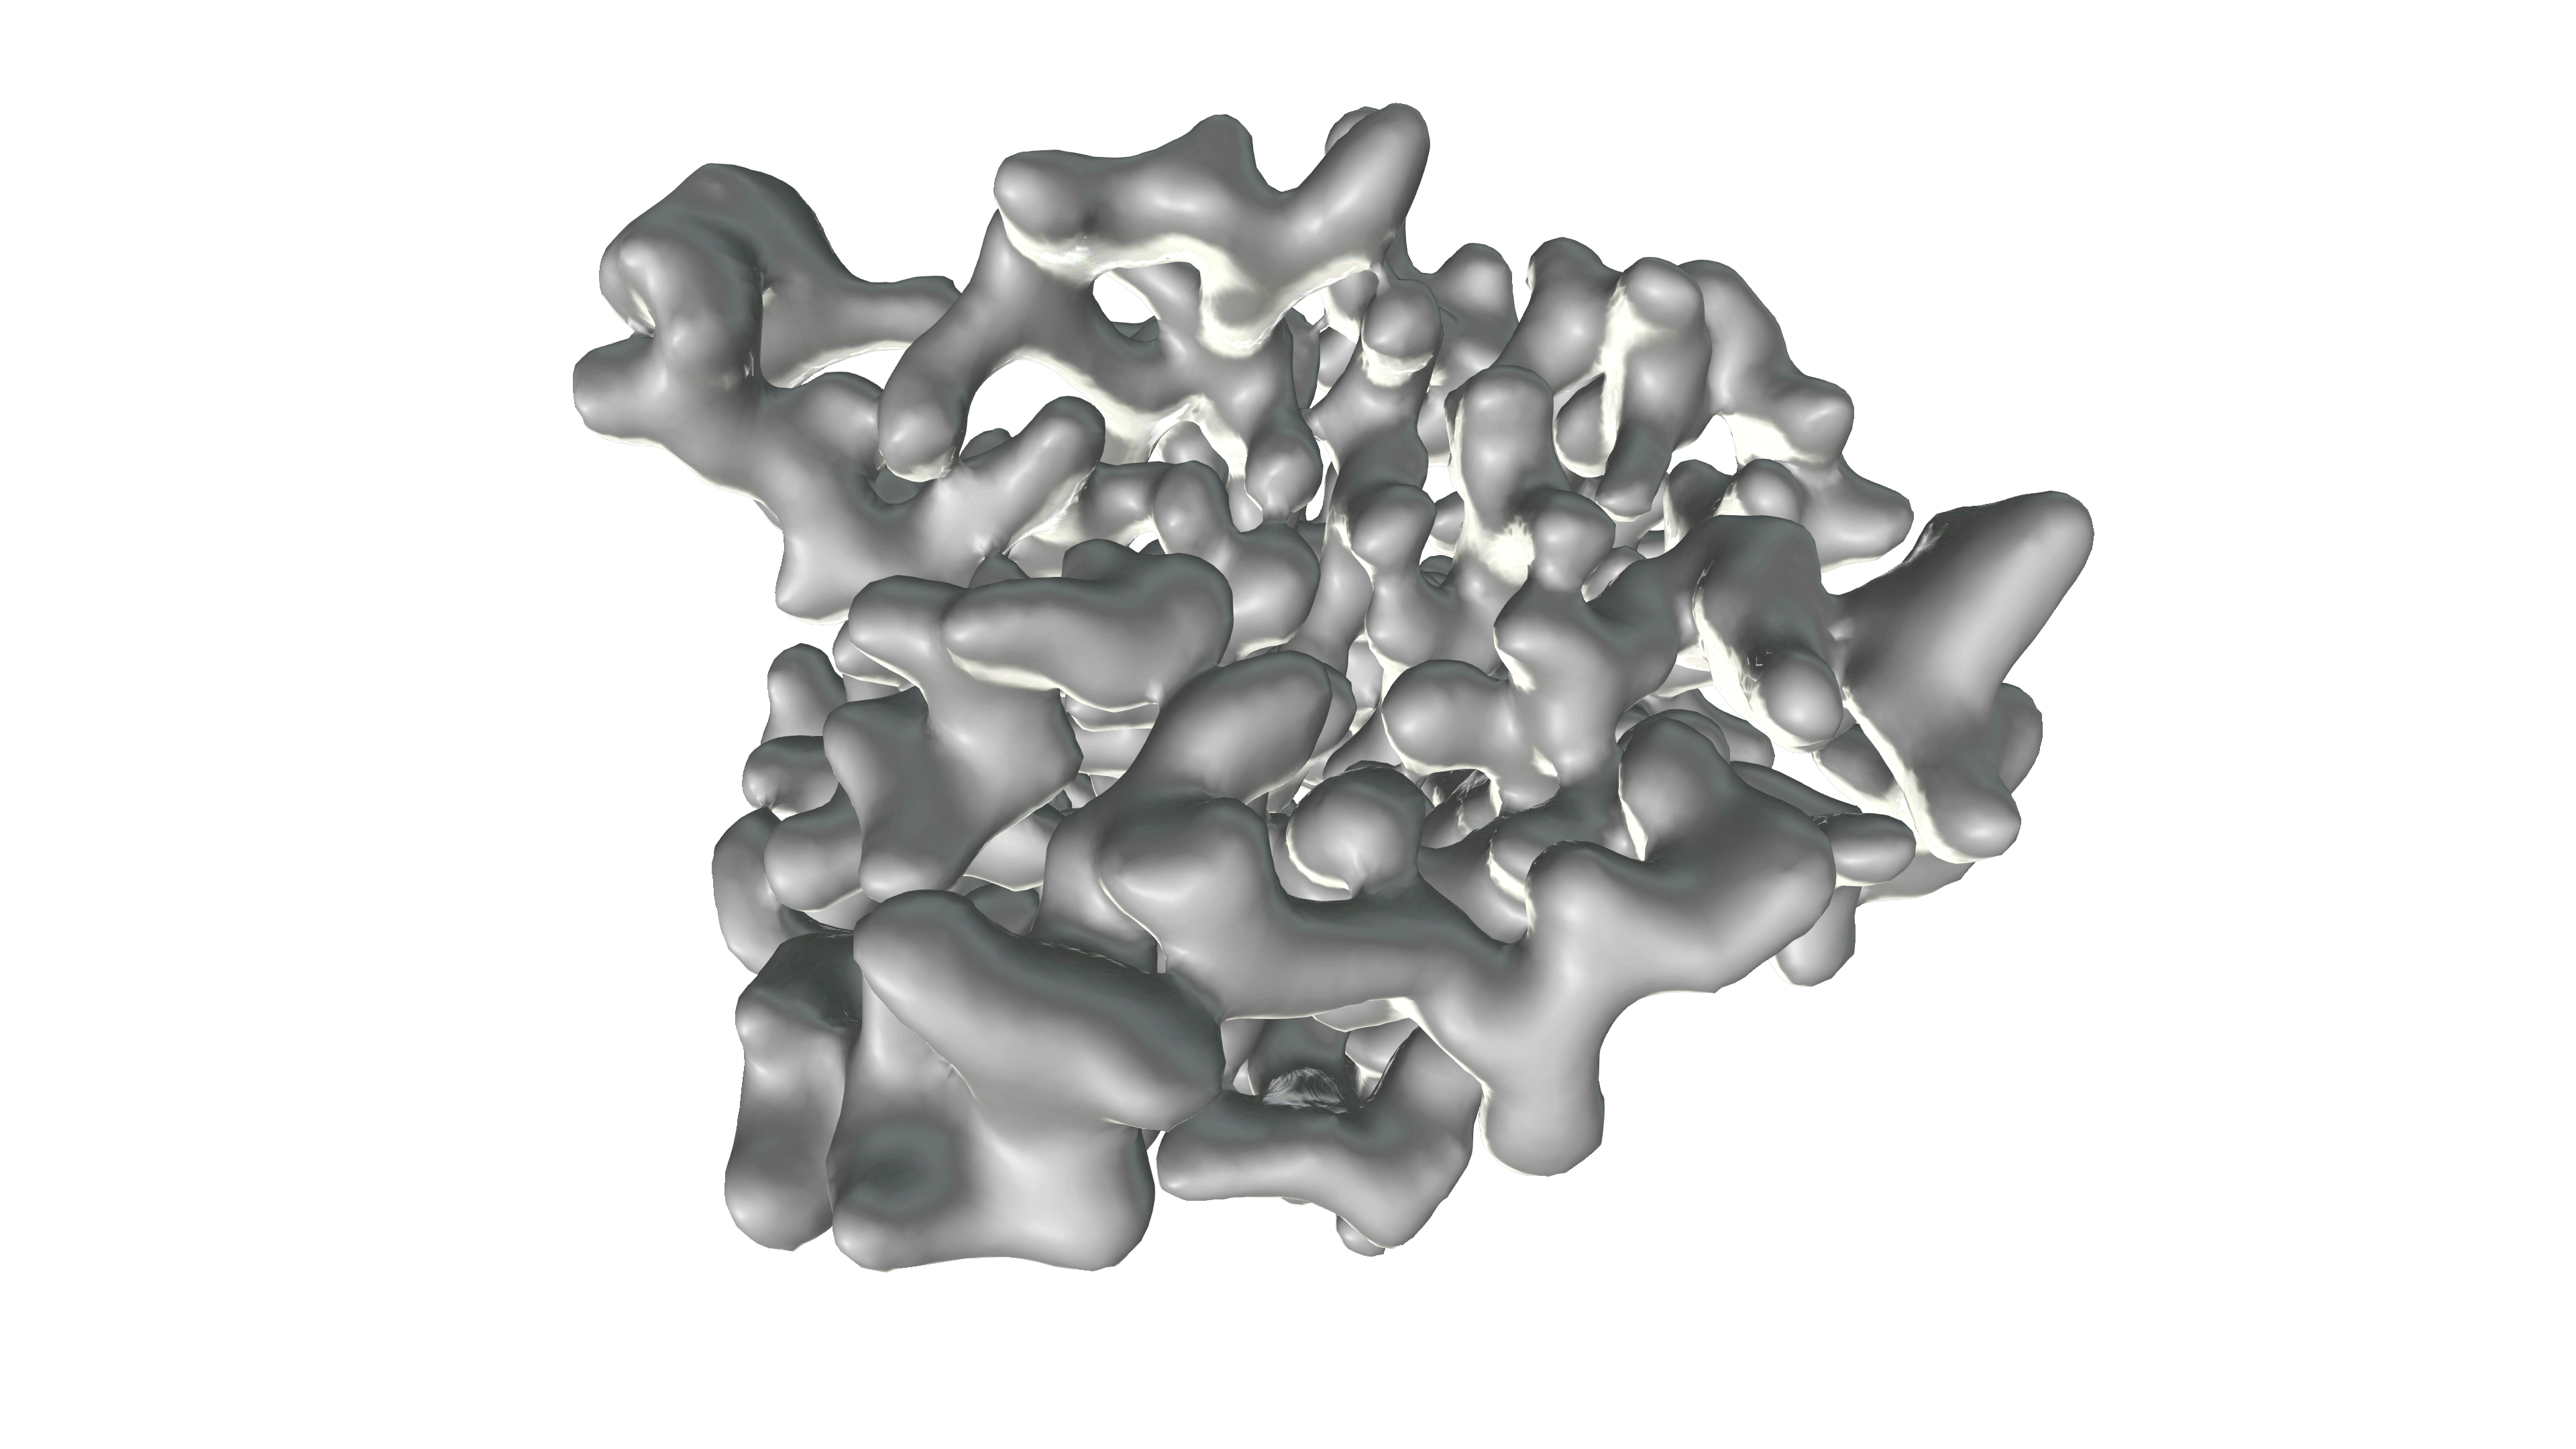
\includegraphics[width=\textwidth]{./figures/ch1/4awn_iso_1_5}
			\caption{Isosurface de densité, avec un seuil élevé, de $1,5$.}
			\label{fig:4awn_iso_1_5}
		\end{subfigure}
		\caption{Désoxyribonucléase (ou ADNase). Cette enzyme est ici illustrée par diverses représentations surfaciques. Illustrations produites par \emph{UnityMol}~\cite{doutreligne2014unitymol} et \emph{Molekel}~\cite{portmann2000molekel, varetto2009molekel} à partir d'une structure de la \emph{Protein Data Bank}~\cite{parsiegla2012structure}.}
		\label{fig:4awn_surf}
	\end{figure}
    
	\subsection{Dynamique moléculaire}
	Une simulation de dynamique moléculaire~\cite{fermi1955alamos, alder1959studies, rahman1964correlations, gibson1960dynamics, lennard1924determination} consiste à simuler, par un calcul numérique, le comportement d'un système moléculaire dans le temps. Celui-ci est modélisé par un système de particules, avec généralement une particule par atome. Des formules mathématiques permettent de modéliser les différentes forces qui s'appliquent à chaque particule, et ces forces sont intégrées avec un pas de temps pour déterminer le mouvement de chaque particule à chaque itération, donc la dynamique du système. L'algorithme général est explicité (quoique sous forme schématique) sur la figure~\ref{fig:moldyn}.
	
	\paragraph{Besoins.} Il est difficile d'observer une macromolécule à l'état statique, et impossible de le faire \emph{in vivo}, lorsqu'elle est en mouvement dans son système naturel. Par conséquent, l'étude de phénomènes moléculaires complexes nécessite de passer par des simulations numériques, seules à même d'en rendre compte. En particulier, la biologie structurale s'intéresse à la \emph{dynamique conformationnelle} des macromolécules (c'est-à-dire à leur conformation tridimensionnelle dans le temps) et à leurs intéractions avec leur environnement --- par exemple le milieu cellulaire. La mise au point de ces simulations s'appuie néanmoins autant que possible sur des données expérimentales.
	
	\paragraph{Initialisation.}
	Une simulation de dynamique moléculaire nécessite une phase d'initialisation. Il faut en premier lieu assigner une position à chaque particule --- chaque atome, en général. Pour ce faire, il est nécessaire de connaître au moins approximativement la conformation de chaque molécule du système. C'est relativement simple pour le solvant, qui est généralement de l'eau avec quelques ions dissous, mais c'est plus compliqué pour les macromolécules dont la conformation n'est pas triviale. Celle-ci est généralement déterminée par une méthode expérimentale telle que la cristallographie aux rayons X, illustrée par la figure~\ref{fig:crystal}. Cette technique fut d'abord employée pour déterminer la structure de petits cristaux inorganiques~\cite{friedrich1912sitzungsberichte, bragg1914reflexion, bragg1913structure, dickinson1923crystal}, puis de molécules organiques et de protéines~\cite{de1925interpretation, crowfoot1935x, kendrew1958three}. Lorsque la cristallographie n'est pas possible, d'autres méthodes, souvent moins précises, peuvent être utilisées. C'est notamment le cas de la spectroscopie de résonance magnétique nucléaire~\cite{clore1989determination, wuthrich1990protein, clore1991structures, wuthrich2001way}. La cryo-microscopie électronique~\cite{adrian1984cryo} (ou cryo-ME, ou encore \emph{cryo-EM} dans la littérature anglo-saxonne) est de plus en plus utilisée~\cite{kuhlbrandt2014cryo, callaway2015revolution}, notamment du fait de ses moindres contraintes --- pas de cristallisation nécessaire --- et de sa résolution croissante~\cite{dellisanti2015barrier, bartesaghi20152}.
	
	Parfois, on procède également par homologie~\cite{marti2000comparative, kaczanowski2010similar}. La modélisation par homologie repose sur l'identification d'une ou plusieurs structures protéiques connues et proches de la séquence d'acides aminés recherchée. Elle passe par un alignement qui établit une correspondance entre les acide aminés de la protéine étudiée et ceux des structures protéiques connues. Cela repose sur l'observation que la structure tridimensionnelle de protéines homologues est mieux conservée que la séquence d'ADN qui l'engendre. La connaissance de la séquence d'acides aminés d'une protéine permet donc d'essayer de prédire sa conformation 3D, si l'on parvient à trouver des protéines homologues dont la structure est connue.
	
	\begin{figure}[H]
		\centering
		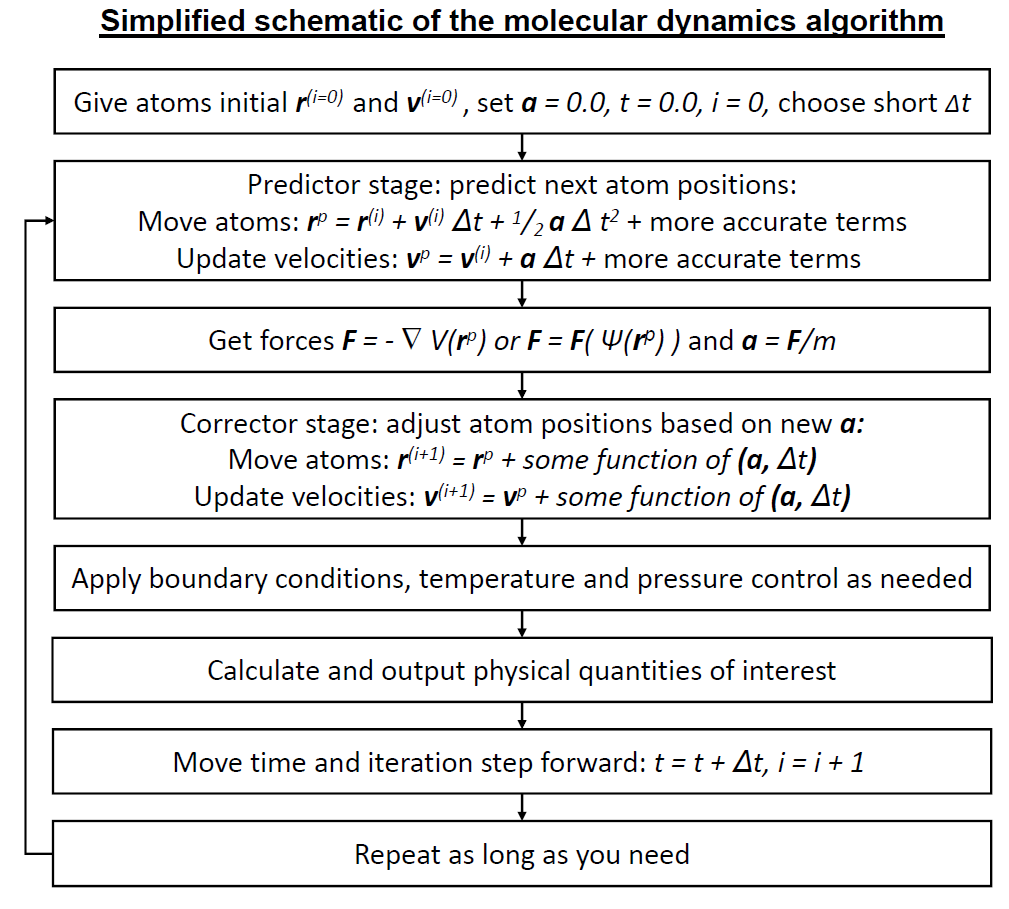
\includegraphics[width=\textwidth]{figures/ch1/moldyn}
		\caption{Schéma simplifié de l'algorithme standard de simulation de dynamique moléculaire. En général, les forces utilisées sont sous forme de potentiels interatomiques classiques ($F = -\nabla V\left(r^{p}\right)$). Ici, $r^{i}$ représente une position à l'itération $i$, $v^{i}$ représente une vélocité à l'itération $i$, $a$ est l'accélération, $t$ est le temps, et $i$ est l'itération. Enfin, $\delta{}t$ est le pas de temps utilisé pour la simulation --- qui doit être suffisamment court pour gérer correctement les phénomènes les plus fugaces, tels que les oscillations des liaisons covalentes carbone-hydrogène, dont la période est de l'ordre de 10~fs ($10^{-14}$~s). Crédit : \emph{Wikimedia}.}
		\label{fig:moldyn}
	\end{figure}
	
	\begin{figure}[H]
		\centering
		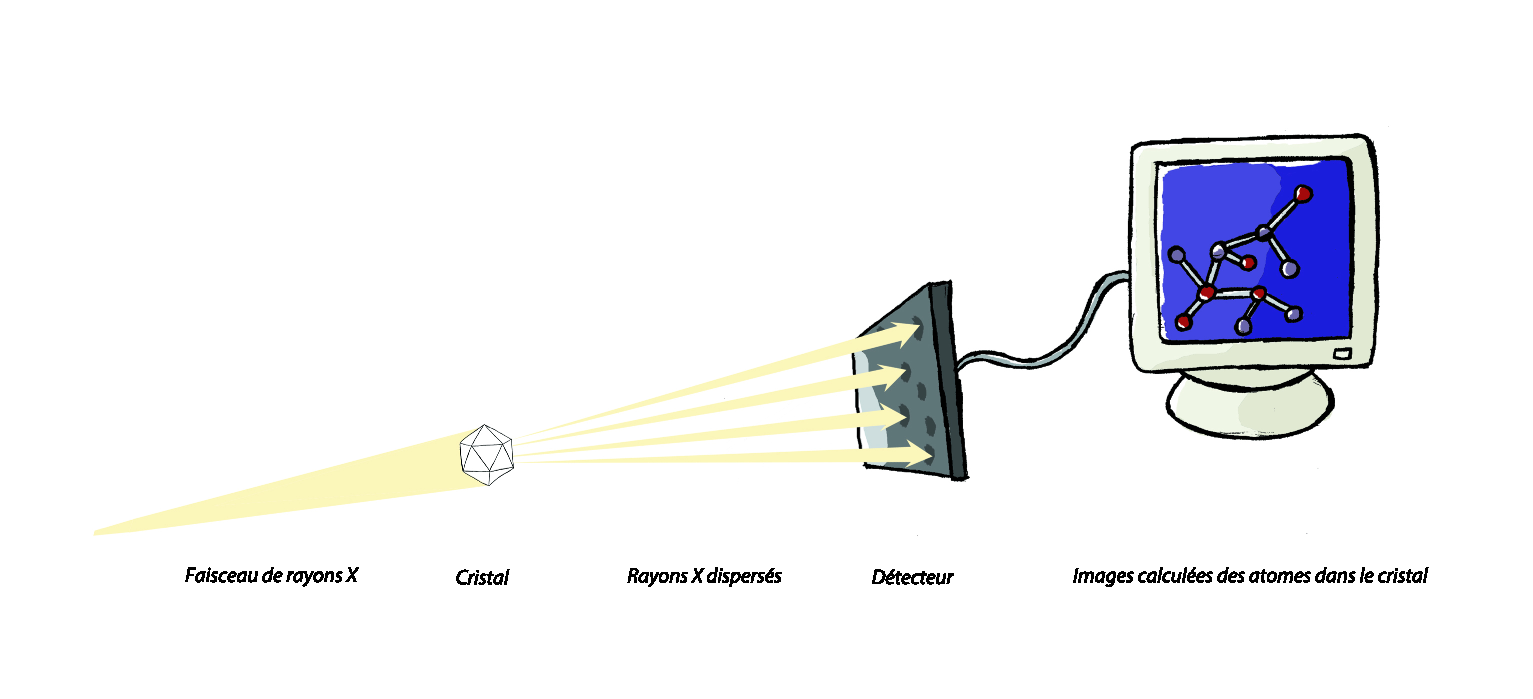
\includegraphics[width=\textwidth]{figures/ch1/crystal}
		\caption{Schéma très simplifié de la cristallographie aux rayons X. Ces rayons traversent un cristal (contenant une même molécule présente en grande quantité) qui les diffracte avant leur capture par un détecteur connecté à un ordinateur. Ce dernier, à l'aide d'un algorithme approprié, en déduit la conformation 3D de la molécule cristallisée. Crédit :~\cite{trellet2015exploration}.}
		\label{fig:crystal}
	\end{figure}
	
	\paragraph{Périodicité.}
	L'espace de simulation est généralement modélisé par ce qu'on appelle des conditions périodiques aux limites~\cite{cheatham1995molecular} (CPL, en anglais \emph{periodic boundary conditions} --- PBC). Elles constituent un ensemble de conditions aux limites utilisées afin de simuler un système pavé effectivement infini. En effet, si un système microscopique est simulé dans le vide, les molécules du système s'évaporeront, s'éloignant les unes des autres à moins d'être maintenues ensemble par une force restrictive externe. Si, au contraire, le système est simulé en utilisant des murs réflecteurs aux limites, des forces parasites sont introduites dans la simulation, pouvant donc créer un écart supplémentaire (en plus des approximations de simulation utilisées) par rapport au système réel.
	
	On optera donc généralement pour un système périodique, comme celui représenté sur la figure~\ref{fig:period} --- ce dernier est en deux dimensions, mais le principe en trois dimensions est le même. Il convient toutefois de prendre des précautions avec les conditions périodiques, afin d'éviter que des interactions \og artificielles \fg{} se produisent entre les \og bords \fg{} de l'espace de simulation, notamment entre les particules et leurs propres images si cela ne correspond pas au système étudié dans son état naturel~\cite{de1997effect}. L'utilisation de formes plus complexes que des parallélépipèdes peut permettre de minimiser ces effets indésirables pour un volume de simulation donné ; les octaèdres tronqués sont une des options possibles, comme l'illustre la figure~\ref{fig:octa}.
	
	\begin{figure}[H]
		\centering
		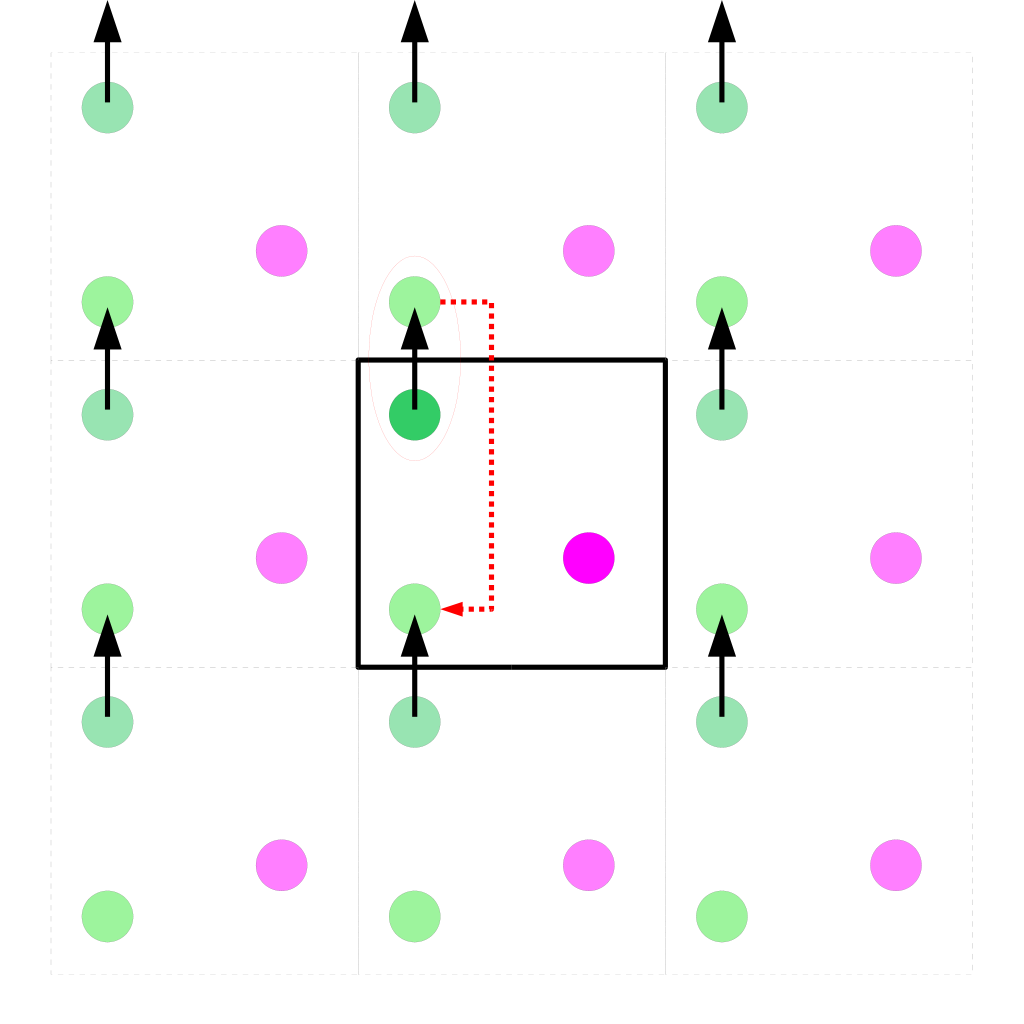
\includegraphics[width=\textwidth]{figures/ch1/period}
		\caption{Comportement par périodicité (2D) : la particule vert foncé (coin supérieur gauche de la boîte en traits pleins) possède une quantité de mouvement l'amenant à sortir de la boîte (flèche). Une fois sortie, la périodicité du système ramène une particule identique dans la boîte, avec la même quantité de mouvement. La particule subit l'influence de toutes les particules environnantes, y compris ses propres images. Crédit : \emph{Wikimedia}.}
		\label{fig:period}
	\end{figure}
	
	\begin{figure}[H]
		\begin{subfigure}{.5\textwidth}
			\centering
			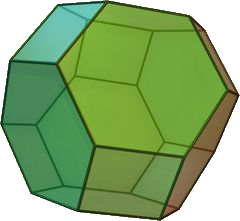
\includegraphics[height=4cm]{./figures/ch1/truncOctahedron}
			\caption{Octaèdre tronqué.}
			\label{fig:truncOctahedron}
		\end{subfigure}
		~
		\begin{subfigure}{.5\textwidth}
			\centering
			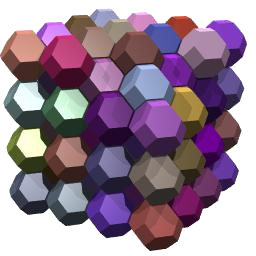
\includegraphics[height=4cm]{./figures/ch1/truncOctahedra}
			\caption{Treillis d'octaèdres tronqués.}
			\label{fig:truncOctahedra}
		\end{subfigure}
		\caption[Octaèdres pour les conditions périodiques aux limites.]{Utilisation d'octaèdres pour la mise en œuvre de conditions périodiques aux limites en minimisant les erreurs et les calculs nécessaires. Crédit : S.R. Saunders, \emph{Real Wireless}\footnotemark.}
		\label{fig:octa}
	\end{figure}
	
	\footnotetext{\url{https://realwireless.wordpress.com/2008/06/03/}}
	
	\paragraph{Paramètres initiaux.} Le principe de la simulation est de calculer les forces exercées sur chaque particule à chaque itération, et d'intégrer ces forces sur un pas de temps donné pour déplacer les particules. Pour pouvoir simuler le comportement du système sur un laps de temps aussi grand que possible --- ce qui est souvent nécessaire pour observer des phénomènes biologiques complexes et longs --- le pas de temps doit être aussi grand que possible. Cela permet en effet à chaque itération de la simulation de couvrir une durée relativement élevée, donc pour un temps (réel) de simulation donné et pour des ressources de calcul données, la durée simulée est maximisée.
	
	Cependant, le pas de temps doit être suffisamment court pour que les événements les plus rapides ne soient pas perdus. Or, les oscillations des liaisons covalentes, par exemple (particulièrement les liaisons carbone-hydrogène) sont très courtes, de l'ordre de $10^{-14}$~s, soit 10 femtosecondes. Le théorème de Nyquist-Shannon~\cite{shannon1949communication} nous apprend qu'il est nécessaire que la fréquence d'échantillonage soit au moins double de la fréquence du signal, aussi le pas de temps doit-il être, au plus, deux fois plus court que la période d'une oscillation de liaison covalente. En pratique, la valeur choisie est généralement de l'ordre de $10^{-15}$~s, soit 1 femtoseconde, du moins pour les simulations de type \og tout atome \fg{} avec liaisons flexibles. Des simulations plus grossières (notamment avec liaisons rigides, voire de type \og gros grains \fg{}) peuvent se contenter de pas de temps plus long, au prix d'une précision amoindrie.
	
	D'autres paramètres doivent être initialisés, par exemple les vitesses des particules, qui suivent généralement une distribution de Maxwell-Boltzmann~\cite{maxwell1860v, maxwell1860ii, boltzmann1970weitere, boltzmann2003further}. Il convient également d'ajuster la température, la pression, le nombre de particules, etc., et de déterminer lesquels de ces paramètres doivent être maintenus constants, et comment. Le changement d'un seul de ces paramètres mènera généralement à une autre exploration de l'espace conformationnel, c'est-à-dire à une trajectoire différente.
	
	\paragraph{Champs de force.}
	Une simulation de dynamique moléculaire s'appuie sur un \emph{champ de force}. Cette notion, propre à la chimie, est à ne pas confondre avec son homonyme en physique. Ce que l'on appelle ici un champ de forces est un ensemble de potentiels et de paramètres permettant de modéliser les interactions entre les particules simulées. Généralement, la forme fonctionnelle de base d'un champ de force s'appuie sur l'équation suivante (également illustrée par la figure~\ref{fig:ffterms}) :
	
	\begin{equation}
		\label{eq:forcefield}
		E_{totale} = E_\text{liée} + E_\text{non-liée}
	\end{equation}
	
	\begin{figure}[H]
		\centering
		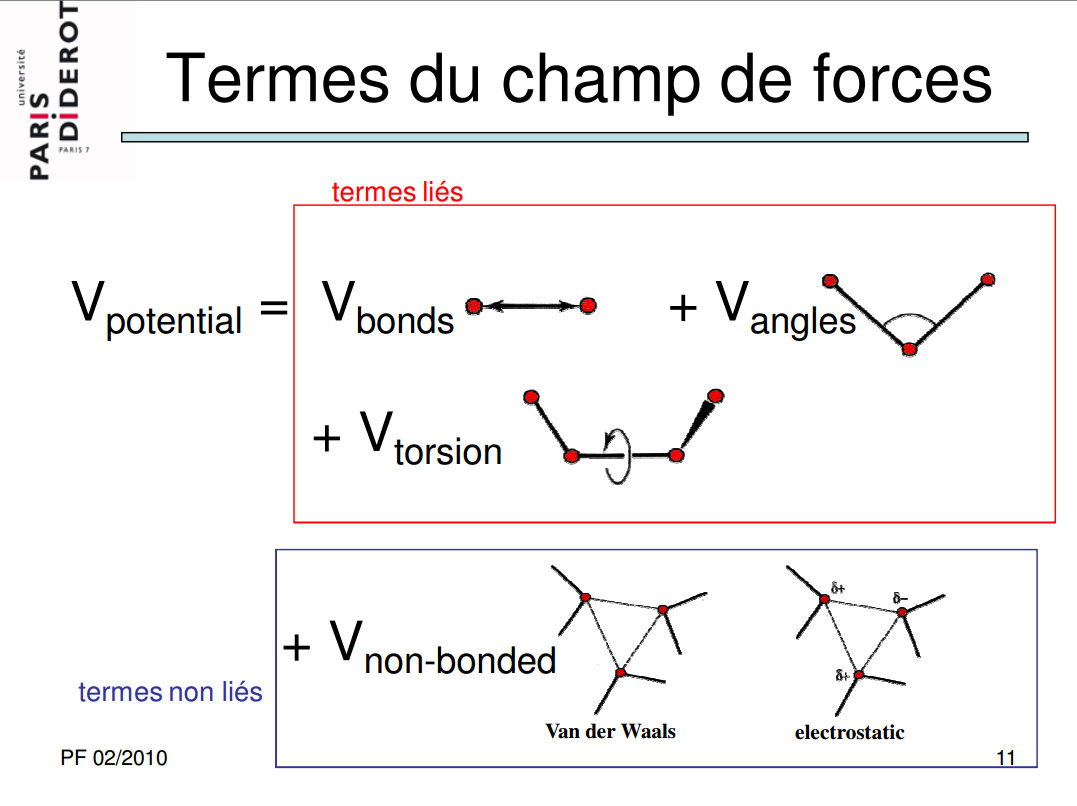
\includegraphics[width=0.7\textwidth]{figures/ch1/ffterms}
		\caption[Termes d'un champ de forces.]{Résumé des termes liés et non liés d'un champ de forces typique. Crédit : Patrick Fuchs\footnotemark.}
		\label{fig:ffterms}
	\end{figure}	
	
	L'énergie totale est égale à l'énergie liée plus l'énergie non-liée, où l'énergie liée représente l'énergie des liaisons covalentes, et l'énergie non-liée représente toutes les autres interactions.
	
	\begin{equation}
		\label{eq:ebonded}
		E_\text{liée} = E_{liaison} + E_{angle} + E_\text{angle\_{}dièdre}
	\end{equation}
	
	Le terme $E_{liaison}$ correspond à l'énergie associée à la variation de la longueur d'une liaison covalente par rapport à son équilibre, comme l'illustre la figure~\ref{fig:e_bond}.
	
	Le terme $E_{angle}$ représente l'énergie associée à la déformation des angles formés par les paires de liaisons covalentes impliquant le même atome, cf. la figure~\ref{fig:e_angle}.
	
	Le terme $E_\text{angle\_{}dièdre}$ correspond à l'énergie associée à la \og torsion \fg{} des liaisons covalentes centrales dans des groupes de quatre atomes, ce qu'explicite la figure~\ref{fig:e_dihedral}.
	
	\begin{figure}[H]
		\centering
		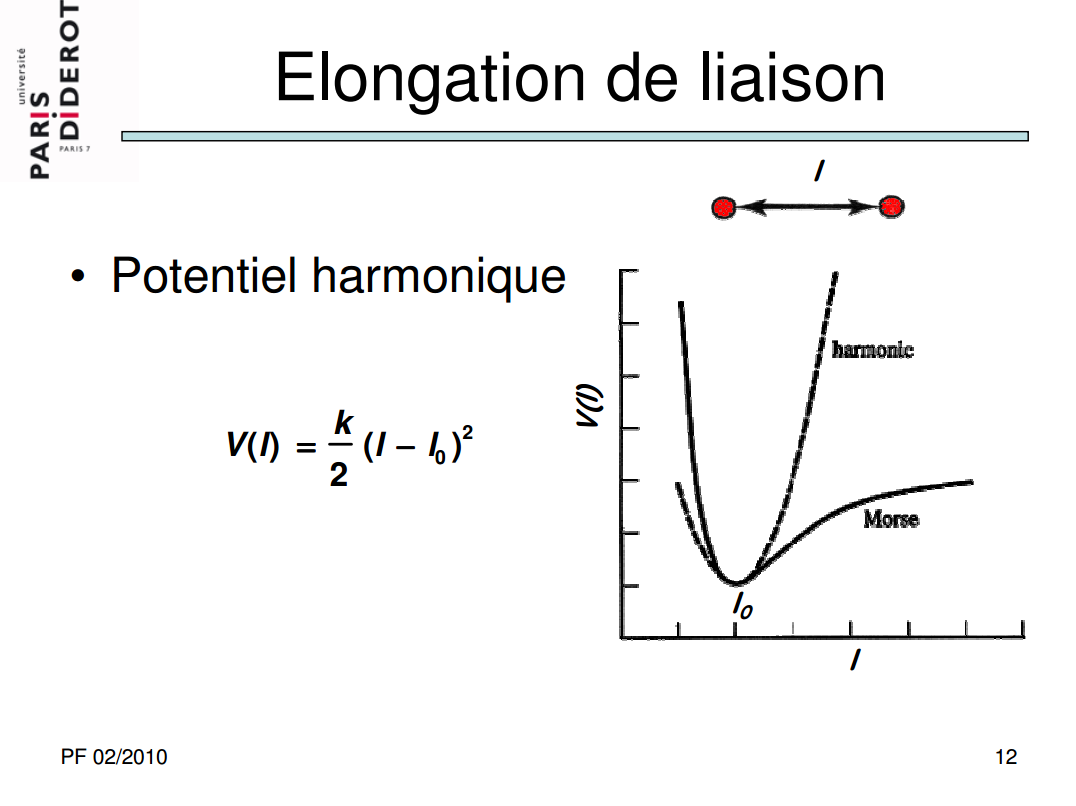
\includegraphics[width=\textwidth]{figures/ch1/e_bond}
		\caption[Énergie de liaison.]{Énergie d'élongation (ou compression) de liaison covalente. Lorsque la longueur de la liaison s'éloigne de son point d'équilibre noté $i_{0}$, l'énergie de liaison augmente. Crédit : Patrick Fuchs\footnotemark.}
		\label{fig:e_bond}
	\end{figure}
	
	\begin{figure}[H]
		\centering
		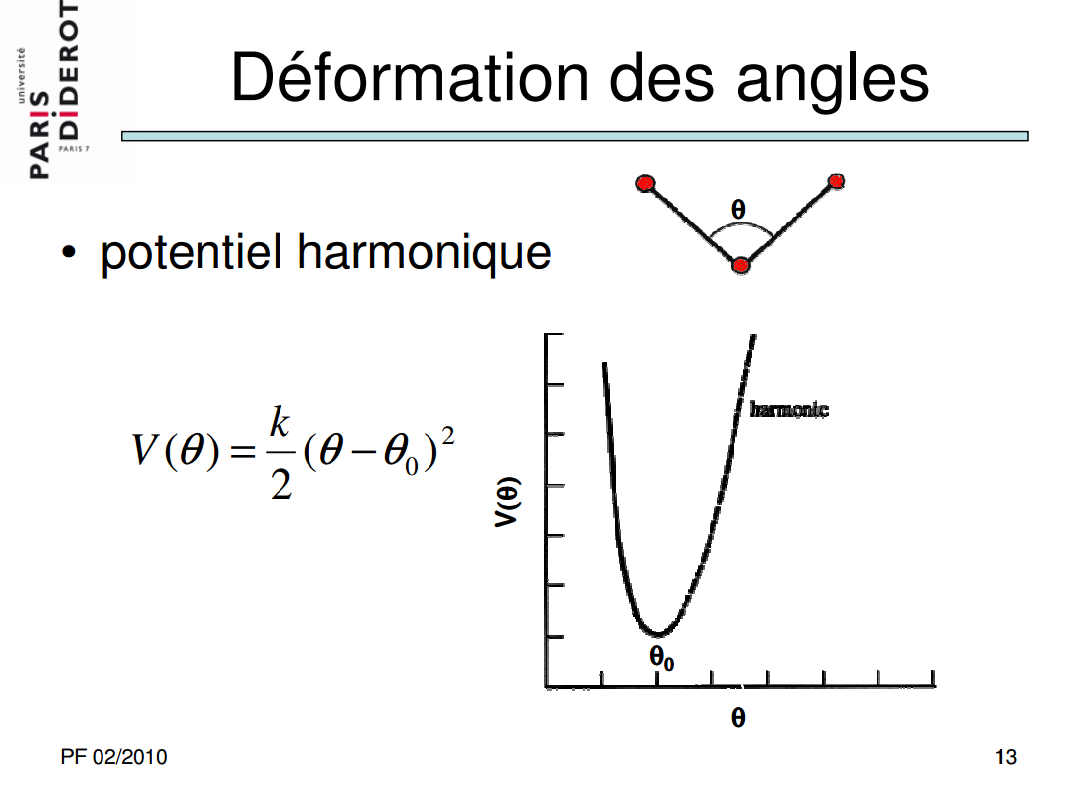
\includegraphics[width=\textwidth]{figures/ch1/e_angle}
		\caption[Énergie d'angle.]{Énergie de déformation des angles formés par des paires de liaisons covalentes impliquant un même atome. Lorsque la valeur de l'angle s'éloigne de son point d'équilibre noté $\theta_{0}$, l'énergie d'angle augmente. Crédit : Patrick Fuchs\footnotemark.}
		\label{fig:e_angle}
	\end{figure}
	
	\begin{figure}[H]
		\begin{subfigure}{\textwidth}
			\centering
			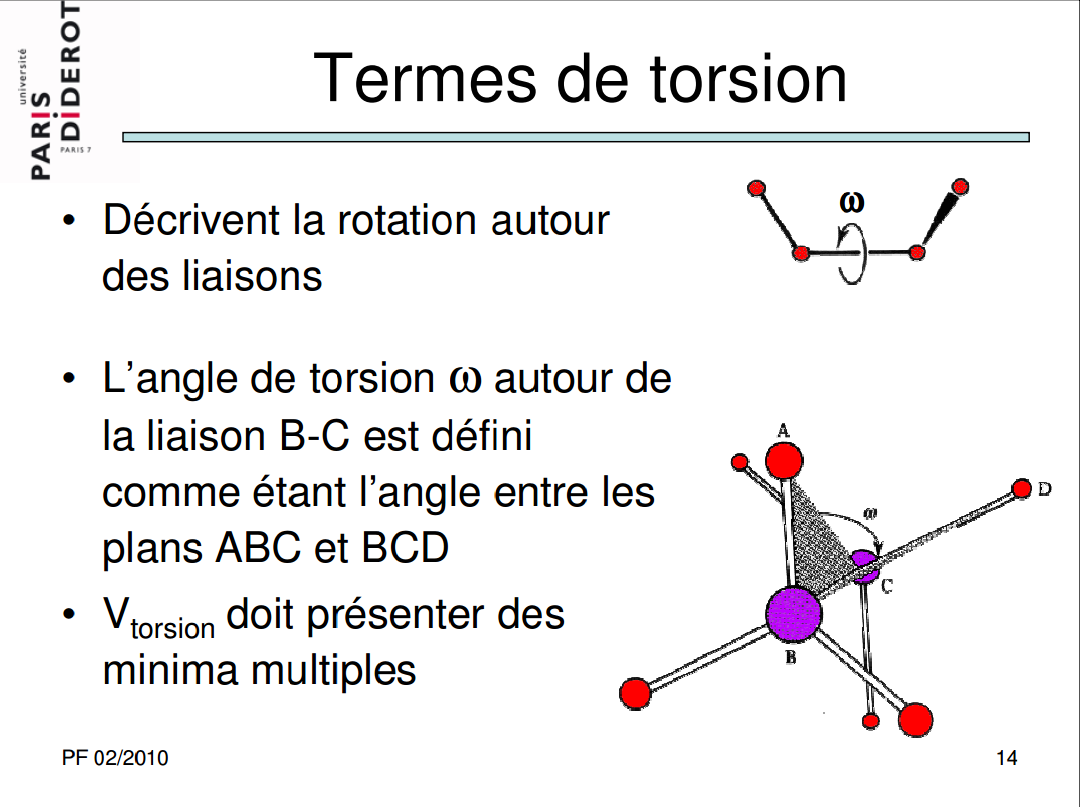
\includegraphics[width=0.8\textwidth]{./figures/ch1/e_dihedral}
			%\caption{}
			\label{fig:e_dihedrala}
		\end{subfigure}
		~
		\begin{subfigure}{\textwidth}
			\centering
			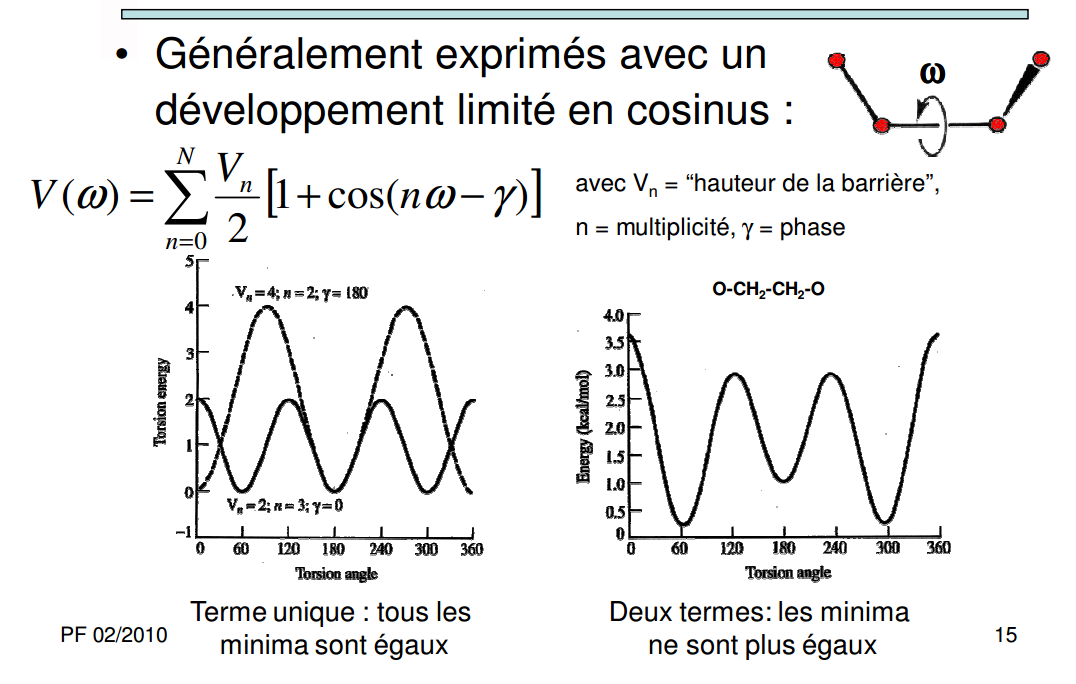
\includegraphics[width=0.8\textwidth]{./figures/ch1/e_dihedralb}
			%\caption{}
			\label{fig:e_dihedralb}
		\end{subfigure}
		\caption[Énergie de torsion, ou d'angles dièdres.]{L'énergie de torsion, ou d'angle dièdre, correspond à la variation des angles illustrés ci-dessus par rapport à leurs valeurs à l'équilibre, qui sont ici multiples. Crédit : Patrick Fuchs.}
		\label{fig:e_dihedral}
	\end{figure}
	
	\begin{equation}
		\label{eq:nonbonded}
		E_\text{non-liée} = E_\text{électrostatique} + E_{van der Waals}
	\end{equation}
	
	Le terme $E_\text{électrostatique}$ représente l'énergie des interactions électrostatiques entre les paires d'atomes ne partageant pas de liaison covalente, telle que la décrit la loi de Coulomb~\cite{coulomb1785premier}. Ce terme est détaillé par la figure~\ref{fig:e_electrostat}. En pratique, une sommation d'Ewald, basée sur une transformation de Fourier, est souvent utilisée avec la loi de Coulomb pour le calcul des énergies électrostatiques~\cite{ewald1921berechnung, essmann1995smooth}.
	
	Le terme $E_\text{van der Waals}$ correspond à l'énergie associée aux forces de van der Waals, déjà décrites plus haut, et résumées par la figure~\ref{fig:e_vdw}.
	
	\begin{figure}[H]
		\centering
		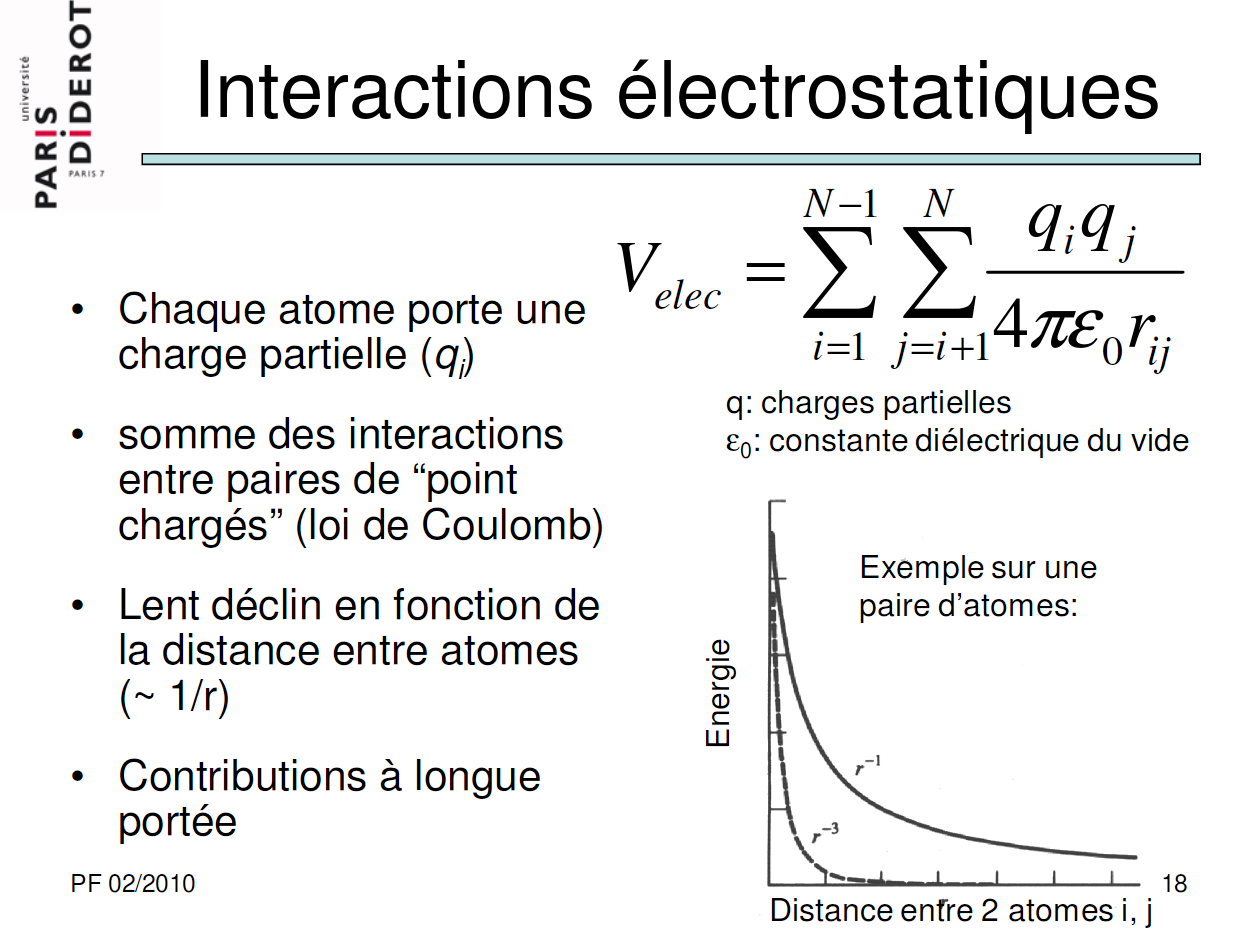
\includegraphics[width=\textwidth]{figures/ch1/e_electrostat}
		\caption[Énergie liée aux interactions électrostatiques.]{Énergie associée aux interactions électrostatiques entre les paires d'atomes non liés. Elle est inversement proportionnelle à la distance entre les atomes. Crédit : Patrick Fuchs\footnotemark.}
		\label{fig:e_electrostat}
	\end{figure}
	
	\begin{figure}[H]
		\centering
		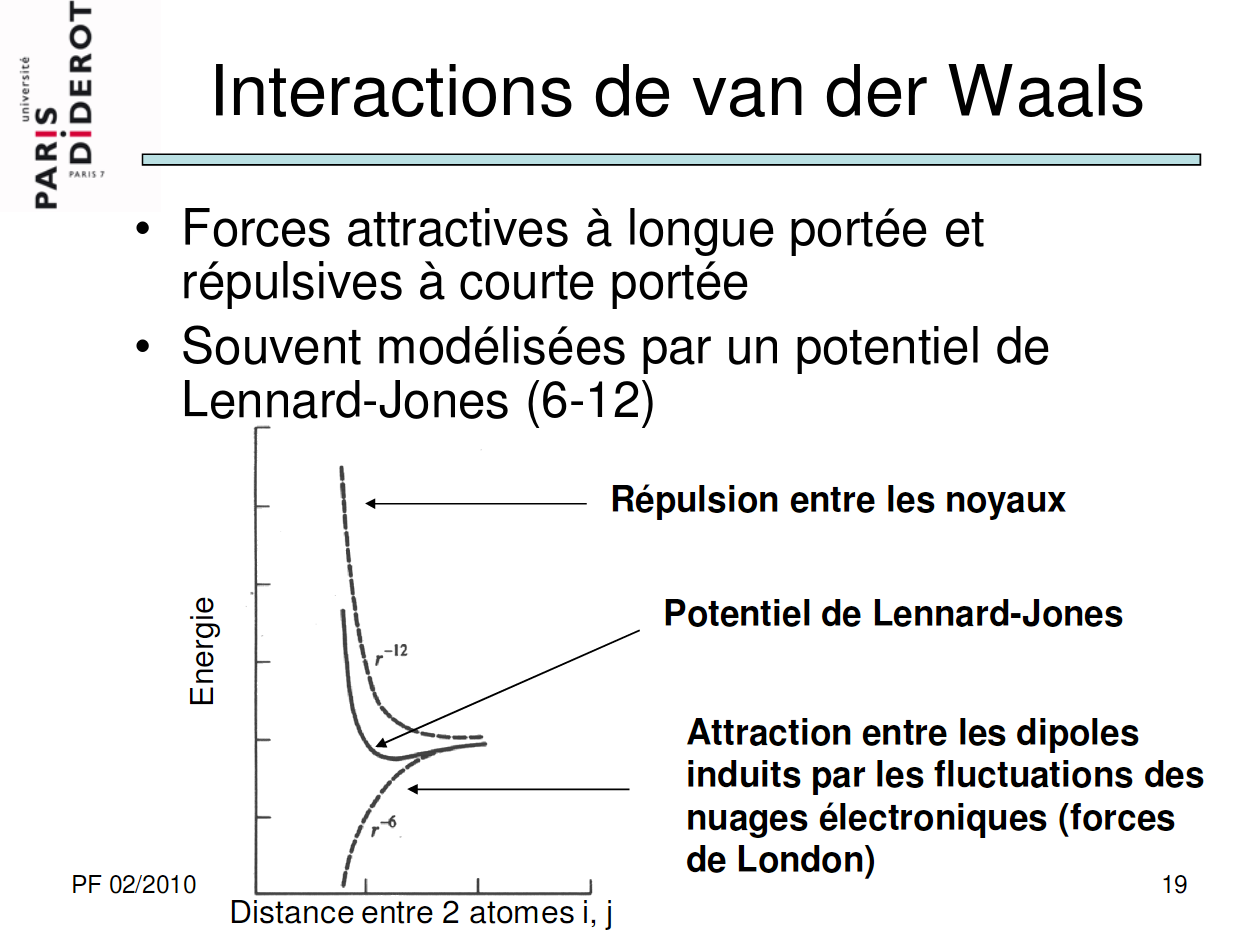
\includegraphics[width=\textwidth]{figures/ch1/e_vdw}
		\caption[Énergie liée aux forces de van der Waals.]{Énergie associée aux forces de van der Waals entre les paires d'atomes non liés. Crédit : Patrick Fuchs\footnotemark.}
		\label{fig:e_vdw}
	\end{figure}
	
	\footnotetext{\url{http://www.dsimb.inserm.fr/~fuchs/M1BC2T/Cours1_FF.pdf}}
	
	Il existe de très nombreux champs de force, avec chacun ses avantages et inconvénients spécifiques, mais parmi les plus couramment utilisés, on peut citer \emph{Chemistry at HARvard Molecular Mechanics} (CHARMM)~\cite{brooks1983charmm, brooks2009charmm}, \emph{Assisted Model Building and Energy Refinement} (AMBER)~\cite{cornell1995second, wang2004development}, \emph{Optimized Potential for Liquid Simulations} (OPLS)~\cite{jorgensen1996development, kaminski2001evaluation}, ou encore \emph{GROningen MOlecular Simulation} (GROMOS)~\cite{scott1999gromos, oostenbrink2004biomolecular}.
	
    
	\subsection{Simulations interactives}
	\paragraph{Limites des simulations non interactives.}
	Les processus biologiques dont l'étude nécessite l'emploi de simulations de dynamique moléculaire impliquent souvent des événements relativement longs ou rares, tels que de profonds changements de conformation, ou des transitions d'un état d'équilibre à un autre, comme la liaison ou la rupture de liaison avec un ligand\footnote{En biologie, un ligand est une molécule qui se lie de manière réversible sur une macromolécule ciblée, protéine ou acide nucléique, jouant en général un rôle fonctionnel : stabilisation structurale, catalyse, modulation d'une activité enzymatique, transmission d'un signal. Par exemple, le hème de la myoglobine est un ligand, cf. la figure~\ref{fig:myoglobin}.}. Or, les simulations de dynamique moléculaire étant généralement limitées à quelques dizaines de nanosecondes, ces phénomènes ne sont pas toujours observables ou reproductibles~\cite{phillips2005scalable}.
	
	\paragraph{Steering.}
	Par conséquent, il est utile de pouvoir agir sur une simulation de dynamique moléculaire. Cette technique est souvent appelée \emph{steering} dans la littérature anglo-saxonne et consiste à appliquer des forces externes à une molécule au cours de sa simulation pour explorer ses propriétés mécaniques, ou pour chercher à provoquer les phénomènes mentionnés ci-dessus, trop lents pour les simulations sans \emph{steering}. Ces phénomènes peuvent ainsi être étudiés~\cite{izrailev1999steered, isralewitz2001steered, isralewitz2001steered}. Certains spécialistes~\cite{phillips2005scalable} préfèrent parler d'\emph{Interactive Molecular Dynamics} (IMD)~\cite{stone2001system, grayson2003mechanisms} lorsque les forces sont appliquées en temps réel par l'utilisateur, par opposition au \emph{steering} basé sur des forces dont l'application est préprogrammée.
	
	\paragraph{Simulations en immersion et retour haptique.}
	La figure~\ref{fig:steeredPIT} présente un exemple précoce (1999) d'IMD en contexte immersif. La notion d'immersion fait l'objet de plusieurs définitions, notamment celles citées par J.-M.~Burkhardt \emph{et al.}~\cite{burkhardt2003immersion} :
	
	\begin{displayquote}
	    \textbf{Acception 1.} Dans le langage courant, le terme d'immersion est compris comme \emph{l'exposition de l'utilisateur à un EV au moyen de dispositifs occultant en partie la perception} (surtout visuelle) de l'environnement alentours, pour afficher en lieu et place une image du monde virtuel (visio-casque, salle immersive de type CAVE, etc.). Par extension, on parle d'immersion auditive, haptique, sensorielle etc. Au-delà d'un caractère informel, cette acception comporte deux ambiguïtés. D'une part, deux sémantiques différentes coexistent :
	    \renewcommand{\labelenumi}{\alph{enumi}} % small letters
	    \begin{enumerate}
	        \item l'immersion comme \emph{l'action d'exposer l'utilisateur à un environnement simulé numériquement},
	        \item l'effet avéré ou supposé de cette exposition sur l'utilisateur.
	    \end{enumerate}
	    
	    D'autre part, en se focalisant sur l'aspect d'exposition, cet usage courant tend à centrer le problème sur la recréation d'une image artificielle proche de la situation réelle de référence, et à occulter les éventuelles interactions avec l'information persistante liée à l'environnement physique réel de l'utilisateur.
	    
	    \textbf{Acception 2.} Le développement d'investigations empiriques en termes d'effet de l'immersion sur la cognition et l'apprentissage, nécessitera de définir de mieux en mieux le concept et de préciser les paramètres de sa mesure. Une définition plus formelle de l'immersion correspondrait ainsi au degré et à la qualité avec lesquels l'interface du système contrôle les entrées sensorielles pour chaque modalité de perception et d'action ; l'immersion peut alors se décrire dans les termes des dispositifs logiciels et matériels particuliers utilisés~\cite{burkhardt1999conception}. Le degré d'immersion se caractériserait alors au moins par :
	    \begin{enumerate}
	        \item le sous-ensemble des modalités mises en \oe{}uvre dans l'interaction,
	        \item les propriétés (degré de complétude, qualité, paramètres du signal, etc.) des dispositifs d'interaction pour chacune des modalités visées,
	        \item la cohérence interne et la latence globale de l'information et des réactions délivrées en temps réel par le système,
	        \item les propriétés de l'environnement physique dans lequel se déroule l'expérience.
	    \end{enumerate}
	    
	    Cette acception renvoie à la notion théorique analogue de \og fidélité du stimulus \fg{}~\cite{stoffregen2003nature} proposée pour être un indicateur de la distance entre le monde physique et sa simulation. Le concept d'immersion ainsi précisé ouvre vers la construction de métriques qui permettraient de quantifier, comparer et étudier systématiquement les effets de l'immersion sur la cognition, les performances et la satisfaction des utilisateurs.
	\end{displayquote}
	
	\begin{figure}[H]
		\centering
		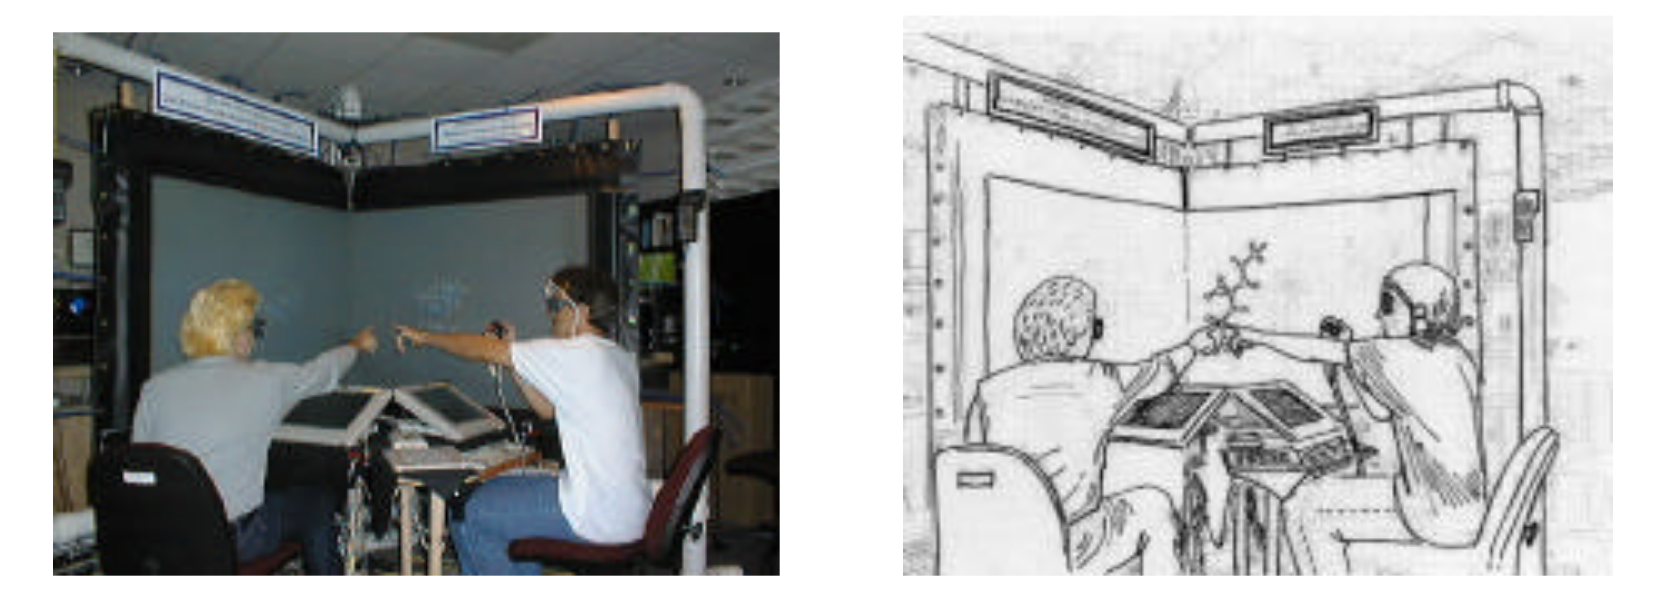
\includegraphics[width=\textwidth]{figures/ch1/steeredPIT}
		\caption[Dynamique moléculaire interactive en environnement virtuel.]{Le logiciel de visualisation moléculaire VMD est utilisé avec les lunettes sétérographiques \emph{CrystalEyes} au sein du système \emph{Protein Interactive Theater} (PIT), qui permet l'immersion dans un environnement virtuel. Le PIT est par ailleurs couplé avec le module de simulation Sigma~\cite{mann2002sigma} pour permettre l'interaction avec la simulation. À gauche, une photo du PIT avec deux utilisateurs. À droite, un schéma de l'environnement virtuel tel qu'il est perçu par les utilisateurs. Crédit :~\cite{prins1999virtual}.}
		\label{fig:steeredPIT}
	\end{figure}
	
	Pour Guillaume Bouyer~\cite{bouyer2007rendu} :
	
	\begin{displayquote}
	    D'un point de vue sensoriel, concret, il s'agit d'occulter partiellement ou totalement la perception de l'humain des objets réels qui l'entourent pour qu'elle soit uniquement ou principalement exposée aux stimuli du monde virtuel. Dans le cas le plus abouti de l'immersion virtuelle, l'humain est totalement découplé du monde réel : seul l'environnement virtuel l'occupe, c'est la notion de \og présence \fg{}. Mais l'immersion peut également être mentale, l'utilisateur pouvant être littéralement \og plongé \fg{}, absorbé par son activité, occultant de lui-même le monde réel (comme il pourrait l'être par exemple pendant la vision d'un film ou la lecture d'un livre). L'immersion de l'utilisateur dans l'[environnement virtuel] est donc créée à la fois par des moyens techniques, sensoriels, comme l'obscurité, de grands écrans et des enceintes diffusant des images en relief et du son 3D, des interfaces de commande non intrusives et naturelles, etc. ; et des procédés logiciels, basés sur des connaissances psychologiques : les concepteurs jouent sur le rendu de la scène, les habitudes de l'utilisateur, ses émotions, etc.
	    
	    Ensuite, l'interaction doit être pseudo-naturelle, c'est-à-dire proche de l'interaction de l'humain dans son environnement réel. En effet, dans le monde réel, l'être humain a acquis, assimilé un certain nombre de \og schèmes \fg{}, de comportements à la fois sensori-moteurs voire cognitifs. Il possède ses propres raisonnements assortis de représentations mentales, a construit une organisation du monde selon un ensemble de règles spatio-temporelles et causales, a acquis des réflexes, a appris des gestes, etc. Dans un [environnement virtuel], il va être tenté de répéter ces schèmes ou de les adapter au nouveau contenu qui s'offre à lui. L'une des caractéristiques des travaux sur l'interaction en RV est de faciliter cette transposition, pour que l'interaction se fasse inconsciemment et sans grand effort mental : \og les interfaces exploitent la motricité ou les perceptions de l'homme issues de son comportement dans le monde réel \fg{}~\cite{fuchs2006introduction}.	
	\end{displayquote}
	
	Pour gérer des données aussi complexes que celles impliquées dans une simulation de dynamique moléculaire, l'immersion présente plusieurs avantages. Comme l'expliquent M.~Dreher \emph{et al.}~\cite{dreher2014exaviz}, le rendu stéréoscopique (\og en 3D \fg{}) permet l'exploration de structures biologiques complexes qui sont intrinsèquement tridimensionnelles. De plus, la stéréoscopie avec suivi des mouvements de la tête permet à l'utilisateur de tourner autour d'objets 3D pour les examiner depuis différents points de vue, simplement en se déplaçant physiquement dans le système immersif, comme dans un contexte réel. Quand ce type de navigation n'est pas nécessaire, la stéréoscopie avec suivi de tête fournit à l'utilisateur la possibilité de se concentrer sur sa structure moléculaire et de l'étudier sous divers angles sans être distrait par les périphériques de navigation ou manipulation traditionnellement utilisés pour pallier le manque d'adaptation du rendu par rapport aux mouvements de tête.
	
	\begin{figure}[H]
		\centering
		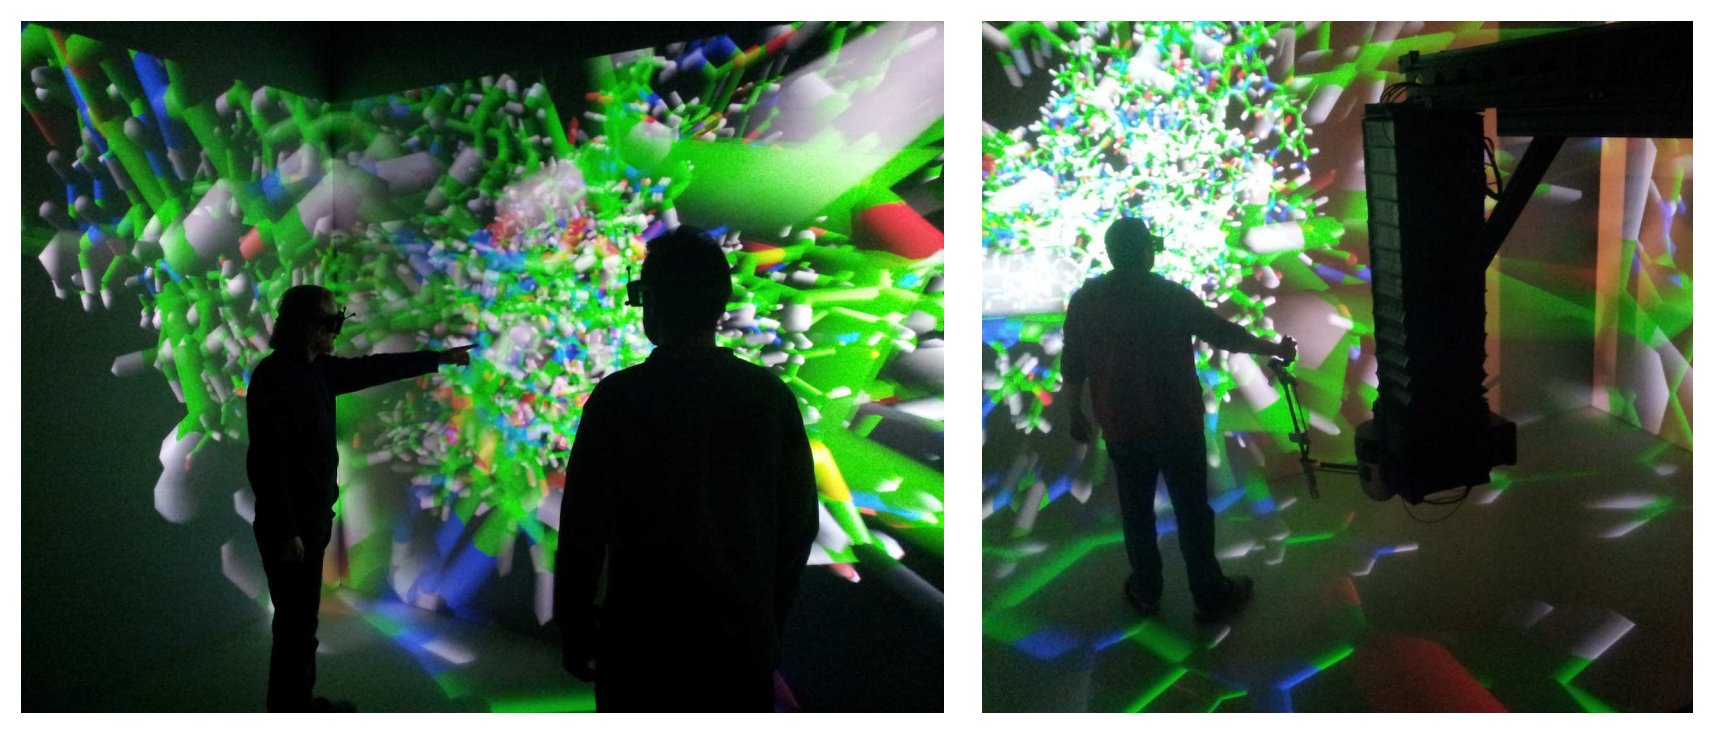
\includegraphics[width=\textwidth]{figures/ch1/exaviz}
		\caption[IMD en environnement virtuel avec retour haptique, \emph{Exaviz}.]{Le système \emph{Exaviz}. À gauche, deux utilisateurs sont dans un CAVE\footnotemark, chacun avec son point de vue personnel en 3D, grâce au suivi de la tête ; ils peuvent ainsi désigner des objets du doigt et en discuter. À droite, l'utilisation du bras haptique permet d'interagir avec les objets de la scène en obtenant un retour de force. Crédit :~\cite{dreher2014exaviz}.}
		\label{fig:exaviz}
	\end{figure}
	
	Pour améliorer la perception des propriétés mécaniques des molécules étudiées, et des forces qui s'exercent sur elle, un retour haptique est possible au cours d'une simulation de dynamique moléculaire interactive~\cite{stone2001system}. Si l'haptique concerne le toucher et les phénomènes kinesthésiques, en pratique on utilise en IMD des bras haptiques, qui fonctionnent par retour de force, comme celui de la figure~\ref{fig:virt6d}.
	
	\begin{figure}[H]
		\centering
		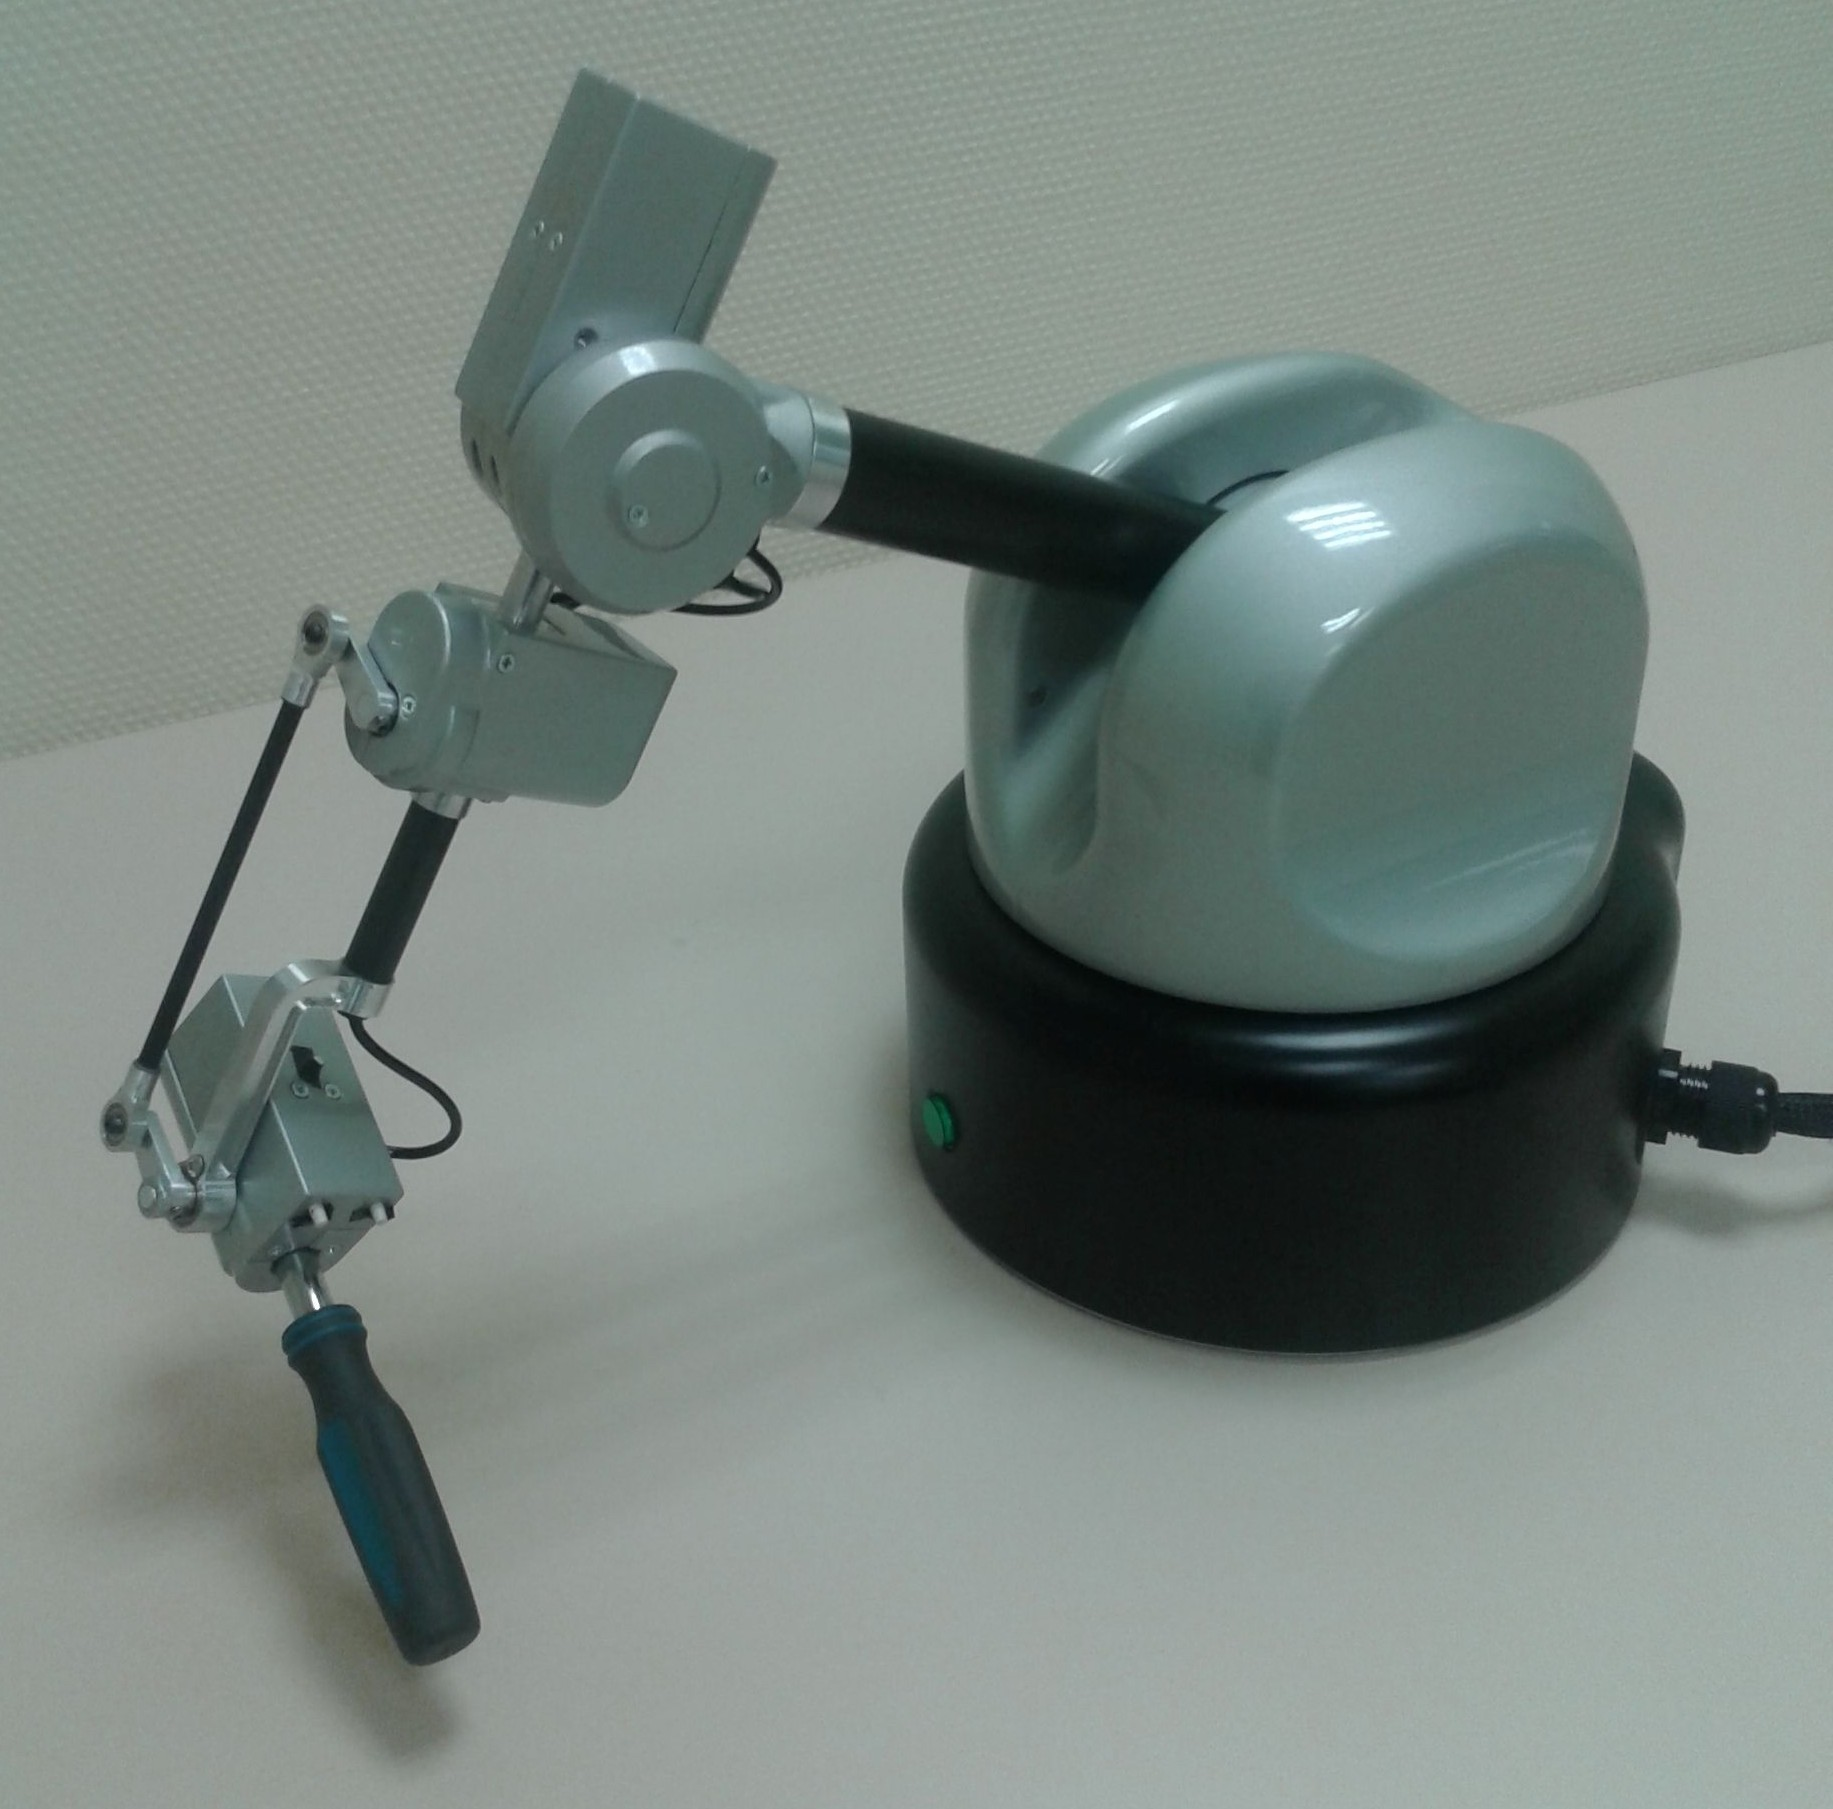
\includegraphics[width=\textwidth]{figures/ch1/virt6d}
		\caption[Bras haptique, Virtuose 6D.]{Le \emph{Virtuose 6D Desktop} est un périphérique haptique conçu pour l'interaction bidirectionnelle avec des environnements virtuels en 3D. C'est un dispositif série dont la structure permet de travailler dans un volume correspondant à un tore de section carrée de 20 cm. Le centre du tore est de 30 cm de la base de l'appareil. La résolution en position est de $4.10^{-2}$ millimètres. Crédit :~\emph{Haption}\footnotemark.}
		\label{fig:virt6d}
	\end{figure}
	
	\footnotetext{\url{http://www.haption.com/site/index.php/fr/products-menu-fr/hardware-menu-fr/virtuose-6ddesktop-menu-fr}}
	
	Ceux-ci peuvent être utilisés de diverses façons, notamment pour percevoir les \og collisions \fg{} entre le curseur et les objets de la scène, ou entre un objet sélectionné par l'utilisateur et un autre objet de la scène, pour permettre à l'utilisateur de percevoir les forces qui s'exercent entre les composantes de la molécule, ou encore pour guider la sélection, en appliquant une force au périphérique haptique dans la direction de la cible présumée de l'utilisateur. Le choix du mode d'utilisation d'un périphérique haptique dans une simulation d'IMD dépend de l'effet recherché.
	
	\footnotetext{\emph{Cave Automatic Virtual Environment}, un système permettant l'immersion dans un environnement virtuel doté de vidéo-projecteurs dirigés vers trois à six des murs d'une salle parallélépipédique. Ce nom est également une référence à l'allégorie de la caverne de Platon, dans laquelle le philosophe médite expose ses vues sur la perception, la réalité et l'illusion.}
	
	\paragraph{Limites et défis actuels.}
	L'interaction avec une simulation de dynamique moléculaire présente plusieurs difficultés majeures. Tout d'abord, le nombre de cibles potentielles est très élevé, avec au minimum plusieurs centaines d'objets, généralement plusieurs dizaines de milliers, voire plusieurs centaines de milliers ou plusieurs millions dans les cas les plus extrêmes. Ces cibles étant confinées dans un espace relativement petit, il en résulte de plus une densité élevée, voire très élevée (selon le mode de représentation). La figure~\ref{fig:exaviz} donne d'ailleurs une idée de cette densité, et encore cet exemple n'est-il pas le plus extrême, car la molécule représentée n'est pas très grande et, surtout, le solvant n'est pas représenté.
	
	Il résulte naturellement de cette forte densité un niveau d'occultation très important. Comme nous l'avons vu plus haut, cette occultation dépend également du mode de représentation utilisé. Le système représenté sur la figure~\ref{fig:gluTrans}, du fait de l'utilisation de sphères de van der Waals, présente un degré d'occultation particulièrement important, et ce malgré le fait que le solvant n'est pas représenté.
	
	\begin{figure}[H]
		\centering
		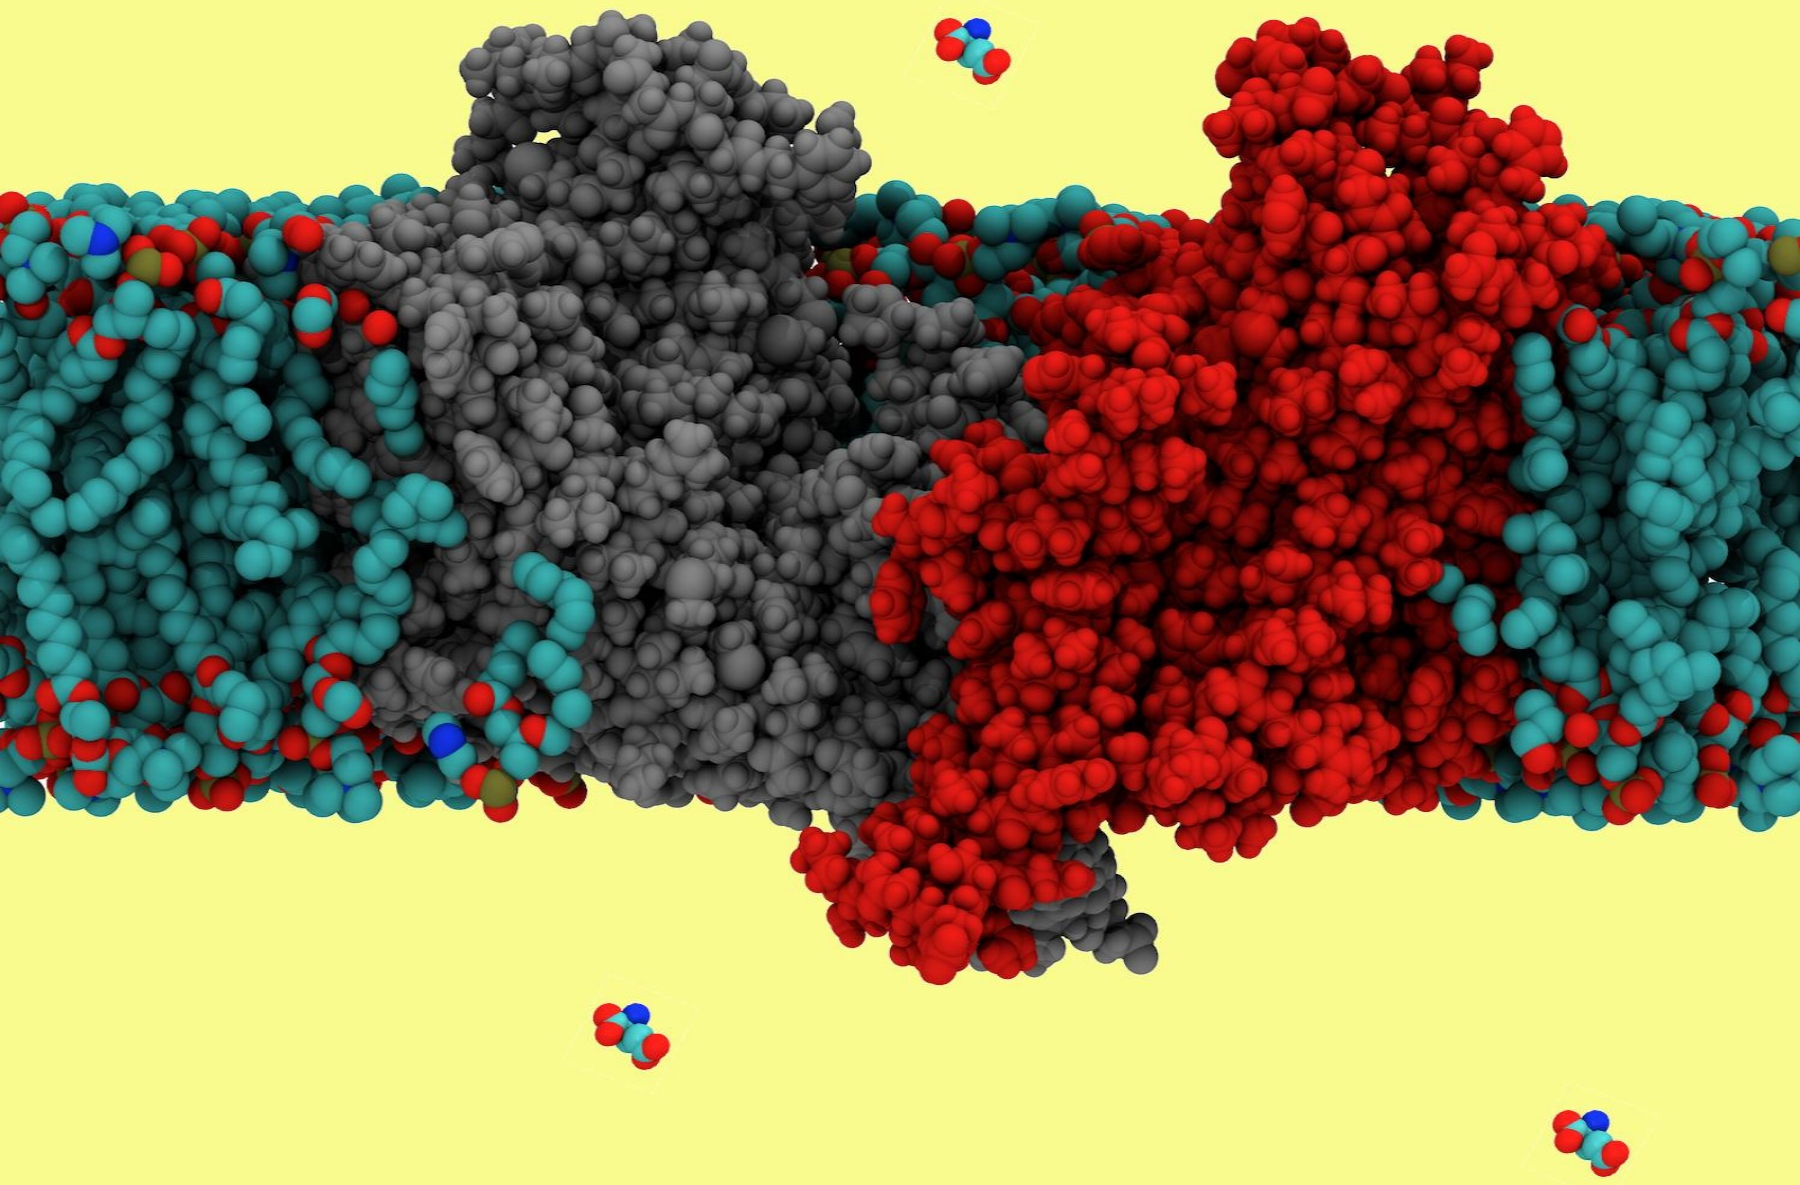
\includegraphics[width=\textwidth]{figures/ch1/gluTrans}
		\caption[Transporteur de glutamate, très forte occultation.]{Un transporteur de glutamate représenté en sphères de van der Waals, sans son solvant. C'est une protéine qui transporte le glutamate (forme ionisée de l'acide glutamique, c'est est le neurotransmetteur excitateur le plus important du système nerveux central) à travers des membranes. Sur cette image issue d'une simulation de dynamique moléculaire, seule la surface de la molécule est visible, les atomes \og enfouis \fg{} sont entièrement occultés, alors qu'ils représentent la majeure partie de la molécule. Crédit : NVIDIA et Joshua Adelman\footnotemark.}
		\label{fig:gluTrans}
	\end{figure}
	
	\footnotetext{\url{https://blogs.nvidia.com/blog/2011/01/13/university-pittsburg-researcher-studies-molecular-dynamics-gpus/}}
	
	Dans les simulations d'IMD, la vitesse des cibles peut être très élevée. Elle dépend en pratique de la vitesse de la simulation, donc de la taille du système simulé et des ressources de calcul disponibles, mais elle peut être supérieure à 10~\r{A}/s, sachant que le rayon d'un atome est d'environ 1~\r{A}.
	
	Quand il s'agit d'interagir avec un tel système, la vitesse d'une particule dans l'espace moteur dépend de la façon dont le système est représenté et du périphérique utilisé, mais elle devient rapidement problématique, \emph{a fortiori} quand la nature même du mouvement pose problème.
	
	En effet, les mouvements des atomes dans une simulation de dynamique moléculaire se caractérisent par leur irrégularité et, par conséquent, leur imprévisibilité. Selon la simulation et la façon dont elle est représentée, les atomes peuvent adopter un mouvement brownien ou plus proche de celui d'une mouche, avec des mouvements très vifs, saccadés et imprévisibles.
	
	Ensemble, la très forte densité de cibles, le haut degré d'occultation, la haute vitesse de ces cibles et la nature très imprévisible de leurs mouvement rendent l'interaction (et en particulier la sélection d'une particule) avec les simulations de dynamique moléculaire très difficile. C'est pourquoi les chercheurs en biologie structurale expriment le besoin de meilleurs modes d'interaction, et c'est la principale motivation des travaux présentés dans cette thèse.
	
	\section{Simulations de problèmes à N corps}
	
	\section{Contrôle de l'espace aérien}
	La biologie structurale n'est cependant pas le seul domaine caractérisé par un besoin d'interaction avec des cibles mobiles, loin s'en faut. La figure~\ref{fig:airtraffic} représente un écran de contrôle du trafic aérien. Les trajectoires des avions sont (normalement) légèrement courbées ou rectilignes, ce qui les rend particulièrement prévisibles, et donc facilite considérablement la tâche de sélection, comme nous le verrons en détail plus loin. Cependant, selon le niveau de zoom et la quantité d'informations contextuelles affichées sur l'écran, le niveau d'occultation peut devenir très important. La vitesse des cibles dépend également du niveau de zoom, mais dans une relation inverse : plus l'échelle est grande, plus les mouvements des avions seront lents sur l'écran.
	
	\subsection{Applications civiles}
	\paragraph{Avions.}
	Quantitativement, un avion de ligne atterrit à environ 250~km/h et ne dépasse pas 1000~km/h en vol de croisière. Ses changements de direction sont très progressifs, généralement de l'ordre de deux degrés par seconde. Ils sont peu fréquents et généralement prévisibles car ils ont pour but d'emprunter des couloirs aériens, ou des trajectoires d'approche imposées aux abords des aéroports. Ils sont néanmoins nombreux, en particulier aux abords des aéroports, et la grande quantité d'informations pertinentes associées à chaque vol peut requérir un affichage contextuel important, d'où une forte densité d'informations, et des niveaux d'occultation parfois élevés. La figure~\ref{fig:atlanta} en fournit un exemple.
	
	\begin{figure}[H]
		\centering
		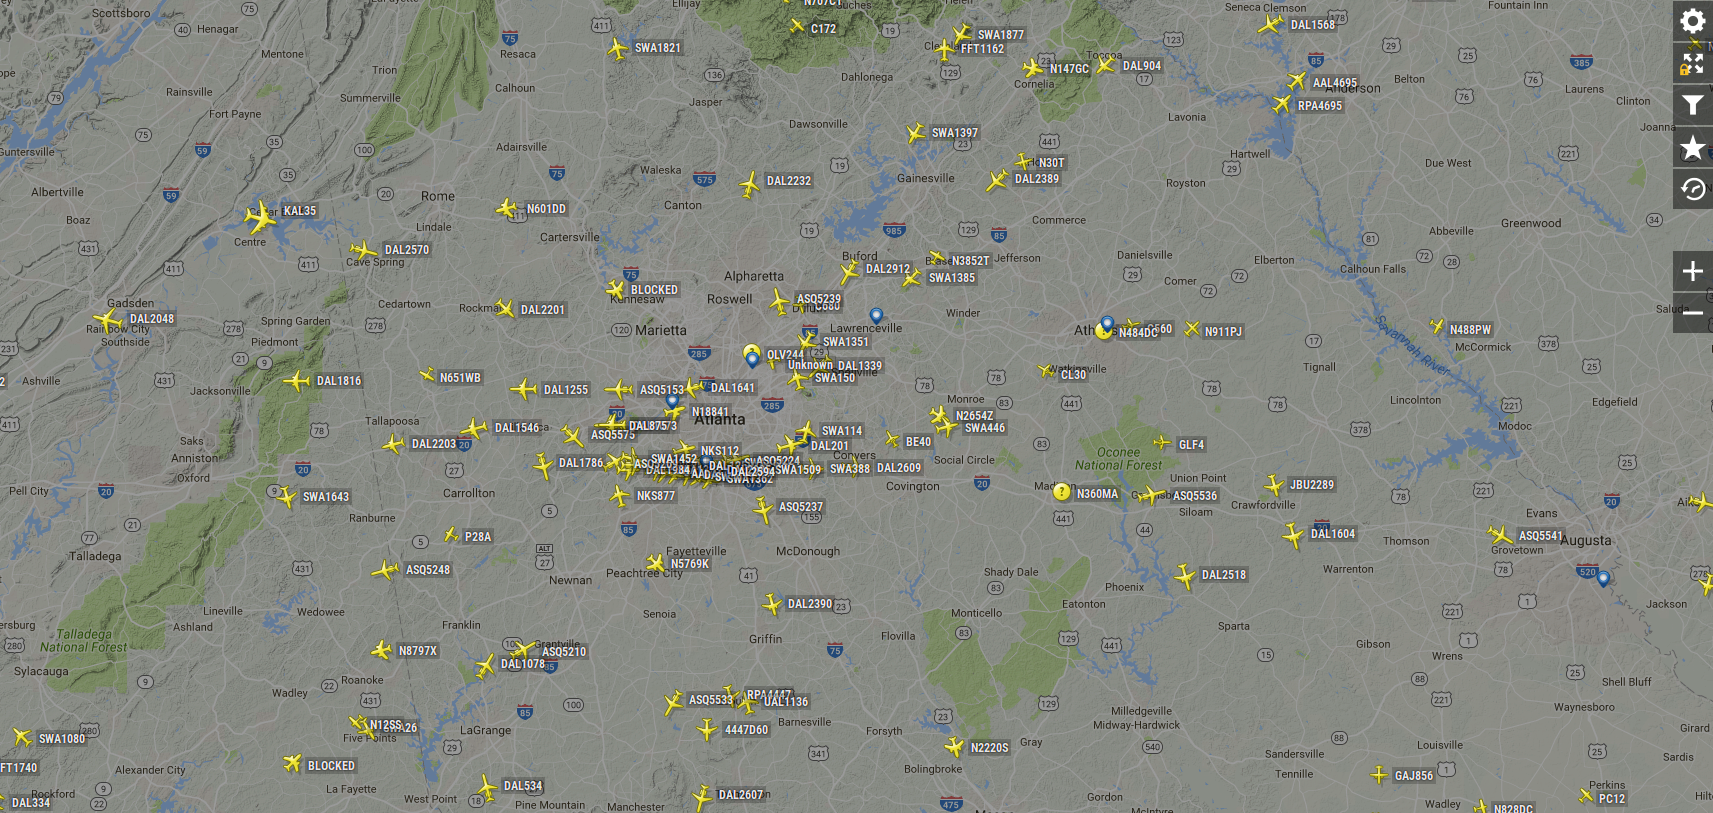
\includegraphics[width=\textwidth]{figures/ch1/atlanta}
		\caption[Trafic aérien, Atlanta.]{Trafic aérien centré sur l'aéroport d'Atlanta, en Géorgie (États-Unis) un lundi matin vers 8~h~40, heure locale. Chaque vol est représenté par un schéma de l'avion permettant d'indiquer son type, ainsi que par un indentifiant de vol alphanumérique, de 5 à 7 caractères. Aucune information supplémentaire (origine ou destination du vol, altitude, vitesse, horaires prévus, modèle exact de l'avion, carburant encore disponible, etc.) n'est affichée ; malgré tout, la densité d'informations est élevée et les appareils s'occultent mutuellement, surtout près de l'aéroport (à quelques kilomètres d'Atlanta, au sud. Néanmoins, les vitesses apparentes (à l'écran) des avions demeurent faibles, sauf à un niveau de zoom élevé. Crédit : \emph{Flight Radar 24\footnotemark}.}
		\label{fig:atlanta}
	\end{figure}
	
	\footnotetext{\url{https://www.flightradar24.com/}}

	\paragraph{Hélicoptères.}
	Comme les aéronefs à voilure fixe, les hélicoptères s'insèrent dans la circulation aérienne et il est nécessaire de les surveiller. Leurs caractéristiques de vol sont néanmoins quelque peu différentes de celles des avions, puisqu'ils peuvent faire demi-tour en environ quatre secondes, voire moins. Ils sont beaucoup plus lents que les avions : les modèles civils dépassent rarement les 300~km/h. La fréquence des changements de direction dépend considérablement de la mission, elle peut être très faible pour un simple transport d'un point A vers un point B, auquel cas la trajectoire de l'hélicoptère va tendre vers la ligne droite, plus importante dans le cadre d'une mission de secours en montagne, et plus importante encore pour un hélicoptère de police fournissant une assistance aérienne pendant une course-poursuite, ou pour un hélicoptère utilisé pour filmer un événement sportif, un documentaire animalier, une manifestation, des émeutes, etc.
	
	\subsection{Applications de sécurité et défense (surveillance de l'espace aérien)}
	Les aéronefs militaires présentent des caractéristiques beaucoup plus variables, dans des intervalles nettement plus grands. C'est notamment dû à leur diversité, puisque l'on trouve des avions de tailles et usages divers, des drones de quelques grammes comme de plusieurs tonnes, des hélicoptères, des missiles, etc.
	
	\paragraph{Avions de chasse.}
	La vitesse d'un avion de chasse, par exemple, peut atteindre 3000~km/h\footnotemark. Il est beaucoup plus difficile d'obtenir des données chiffrées sur la maœuvrabilité de tels engins, mais il est du moins clair qu'un avion de chasse moderne peut changer de direction beaucoup plus brutalement qu'un avion de ligne, et certaines sources non officielles font état de capacités de l'ordre de 35\textdegree{}/s pour les meilleurs\footnotemark.
	
	\addtocounter{footnote}{-1}
	\footnotetext{Données constructeur : \url{http://www.migavia.ru/index.php/en/production/mig-31e-fighter?limit=1&start=2}}
	\addtocounter{footnote}{1}
	\footnotetext{\url{https://defenseissues.net/2014/01/11/comparing-modern-western-fighters/}}
	
	La fréquence maximale à laquelle un avion peut changer de direction est également difficile à connaître avec certitude, d'autant qu'elle dépend de la façon dont on définit un changement de direction, mais une simple observation d'une démonstration en vol permet d'estimer que cette valeur est, grossièrement, de l'ordre d'un changement par seconde environ\footnotemark. Indépendamment des capacités techniques des avions militaires, leurs missions peuvent précisément imposer la recherche de l'imprévisibilité (par exemple pour éviter les tirs ennemis)~\cite{shaw1985fighter} ce qui n'est généralement pas le cas dans le civil.
	
	\footnotetext{Démonstration en vol : \url{https://www.youtube.com/watch?v=vo0ZN2_O29M}}
	
	\begin{figure}[H]
		\centering
		\includegraphics[width=\textwidth]{figures/ch1/AlFursan}
		\caption[La patrouille acrobatique \emph{Al Fursan}.]{La patrouille acrobatique émiratie \emph{Al Fursan}, avec ses trajectoires entremêlées mises en évidence par des traînées de fumée colorées. Des avions militaires peuvent avoir des trajectoires à la fois complexes, très proches les unes des autres, et parcourues à grande vitesse. Crédit : The National UAE\footnotemark.}
		\label{fig:alfursan}
	\end{figure}
	
	\footnotetext{\url{http://www.thenational.ae}}
	
	Il convient de noter que les avions de chasses eux-mêmes ont des besoins similaires en matière de sélection de cibles mobiles, puisqu'ils ont, comme les stations au sol, pour rôle de contrôler l'espace aérien. Ils ont de plus la charge de mener des opérations de reconnaissance ou de bombardement de cibles au sol qui, si elles sont statiques, sont bien mobiles dans le référentiel de l'avion en vol, a fortiori si elles sont filmées par des caméras mobiles. Par ailleurs, les cibles affichées sur les ordinateurs de bord des avions sont accompagnées de diverses informations tactiques qui augmente fortement la densité d'informations, et potentiellement le niveau d'occultation, comme l'illustre la figure~\ref{fig:sitac}.
	
	\begin{figure}[H]
		\centering
		\includegraphics[width=\textwidth]{figures/ch1/sitac}
		\caption[Situation tactique vue d'un \emph{Rafale}.]{Cette image représente une situation tactique telle qu'affichée sur un écran dit \og visualisation tête moyenne \fg{} dans un \emph{Rafale}, un avion de chasse français produit par Dassault Aviation. Sur cette image très \og chargée \fg{} seuls deux petits symboles, que nous avons ici entourés en rouge, représentent des avions ennemis. Au-delà de la carte de fond, les autres symboles représentent diverses informations tactiques importantes : l'avion lui-même bien sûr, sa direction, une boussole, l'altitude maximale des obstacles terrestres, l'échelle, la vitesse de l'avion, le plan de vol, la ligne de front, une loupe, etc. Par conséquent, même avec un très petit nombre de cibles potentielles, l'affichage est complexe, dense, et potentiellement gênant pour la sélection. Crédit : Portail Aviation\footnotemark.}
		\label{fig:sitac}
	\end{figure}
	
	\footnotetext{\url{http://www.portail-aviation.com/2015/07/exclusif-a-la-decouverte-de-la-situation-tactique-du-rafale-sitac.html}}
	
	\paragraph{Hélicoptères.}
	De même, les hélicoptères militaires sont plus agiles que leurs homologues civils, sans qu'il soit aisé de quantifier cette différence. Comme pour les avions, leur comportement est susceptible de varier considérablement selon la mission. Ils sont ausssi légèrement plus rapides, de quelques dizaines de km/h, notamment en piqué. Comme pour les avions, leurs missions impliquent souvent des trajectoires moins prévisibles, d'autant qu'ils cherchent souvent à se camoufler (visuellement et pour les radars) en volant le plus bas possible, ce qui implique de contourner les éléments de relief. L'hélicoptère \emph{Tigre} représenté sur la figure~\ref{fig:tigre} est un exemple d'appareil rapide, compact et très manœuvrable.
	
	\begin{figure}[H]
		\centering
		\includegraphics[width=\textwidth]{figures/ch1/tigre}
		\caption[Hélicoptère d'attaque \emph{Tigre}.]{L'hélicoptère d'attaque \emph{Tigre} conçu et fabriqué par Airbus Helicopters. Cet aéronef est capable de voler jusqu'à 370~km/h en piqué, et il est assez manœuvrable pour changer de direction de vol (sans nécessairement changer l'orientation de l'engin, par exemple en volant latéralement) très rapidement, voler à très basse altitude en suivant le terrain, effectuer des tonneaux, \emph{loopings}, etc., notamment grâce à sa capacité de tolérer des accélérations allant jusqu'à 4g~\cite{tigre}. Crédit : \emph{Wikimedia}}
		\label{fig:tigre}
	\end{figure}
	
	\paragraph{Drones.}
	Le cas des drones aériens, c'est-à-dire des aéronefs sans pilote embarqué (télécommandés ou autonomes) est peut-être le plus hétérogène. On trouve en effet des drones de très petite taille, mais aussi des modèles de plusieurs tonnes~\footnotemark. Leurs modes de sustentation sont très divers, leurs moyens de propulsion varient également et, de fait, leurs caractéristiques de vol sont extrêmement variables, selon qu'il s'agisse de très petits engins extrêmement manœuvrables ou d'aéronefs plus gros, qui se comportent comme des avions traditionnels.

	\footnotetext{On peut citer le RQ-4 \emph{Global Hawk}, de Northrop Grumman, un drone de reconnaissance dont la masse maximale au décollage dépasse les 14 tonnes, ce qui le rend comparable à un avion de chasse.
	\url{http://www.af.mil/AboutUs/FactSheets/Display/tabid/224/Article/104516/rq-4-global-hawk.aspx}}
	
	Au-delà de leurs caractéristiques de vol, certains drones sont délibérément conçus pour être utilisés en grandes quantités, en essaims\footnotemark~\cite{alonso2016distributed, saska2014autonomous}, notamment pour submerger l'ennemi par le nombre. Cela implique une densité de cibles potentiellement très importante, avec les niveaux d'occultation qui en découlent. L'on peut d'ailleurs supposer qu'ils seront impliqués dans des manœuvres délibérément conçues pour compliquer la détection, l'identification et le suivi des drones individuels.
	
	\footnotetext{L'\emph{Office of Naval Research} du \emph{Department of Defense} étastunien ne cache pas son intérêt pour l'usage d'essaims de drones, comme l'illustre ce communiqué de presse intitulé \emph{LOCUST: Autonomous, swarming UAVs fly into the future} : \url{http://www.onr.navy.mil/Media-Center/Press-Releases/2015/LOCUST-low-cost-UAV-swarm-ONR.aspx}.
	
	Le \emph{Strategic Capabilities Office} du même département a déjà mené des essais avec des essaims d'une centaine de petits drones : \url{https://www.washingtonpost.com/news/checkpoint/wp/2016/03/08/watch-perdix-the-secretive-pentagon-program-dropping-tiny-drones-from-jets/} ; \url{https://www.defense.gov/Portals/1/Documents/pubs/Perdix\%20Fact\%20Sheet.pdf}.}
	
	
	
	\begin{figure}[H]
		\centering
		\includegraphics[width=\textwidth]{figures/ch1/swarm}
		\caption{Petit essaim de drones aériens. Ces engins simples et peu coûteux peuvent être produits et utilisés en très grand nombre. Ils sont souvent capables d'évoluer en formation serrée, donc de constituer un ensemble de cibles très dense. Crédit : \emph{International Business Times}\protect\footnotemark.}
		\label{fig:swarm}
	\end{figure}
	
	\footnotetext{\url{http://www.ibtimes.com/}}
	
	Dans une certaine mesure, le contrôle de la circulation des drones est également un enjeu pour le domaine civil, car ils peuvent évoluer (légalement ou non) près des aéroports. Cette pratique peut représenter un risque de sécurité, et des arrêtés ont été pris par le Ministère de l'écologie et du développement durable pour les prévenir, comme le rappelle notamment l'Union des Aéroports Français\footnotemark. Par ailleurs, l'utilisation de drones au-dessus de sites sensibles tels que les centrales nucléaires ne va pas sans inquiéter EDF et les pouvoirs publics\footnotemark.
	
	\addtocounter{footnote}{-1}
	\footnotetext{\url{http://www.aeroport.fr/page/page/drones}}
	
	\addtocounter{footnote}{1}
	\footnotetext{\emph{Au total, 17 sites nucléaires ont été survolés par des drones depuis octobre [2014, au 29 janvier 2015]} : \url{http://www.lemonde.fr/planete/article/2015/01/29/dix-sept-sites-nucleaires-ont-ete-survoles-par-des-drones-depuis-octobre_4565967_3244.html}}


	Les drones représentent un risque sécuritaire généralisé :
	
	\begin{displayquote}
	C'est un mode d'action inédit contre des forces françaises. Le camp militaire d'Erbil, qui abrite des peshmergas et des commandos français au Kurdistan irakien, a été le théâtre d'une explosion sans précédent le 2 octobre dernier. Celle d'un drone, piégé par le groupe État islamique. Bilan : deux combattants kurdes tués, et deux commandos parachutistes de l'armée de l'air française grièvement blessés.
	
	[\ldots{}]
	
	\og On ne peut pas faire grand-chose \fg{}, constate avec amertume auprès de LCI Jean-Vincent Brisset, général de brigade aérienne. Ce directeur de recherche à l'IRIS l'assure : \og C'est quelque chose d'assez terrifiant pour les services de sécurité. Il est horriblement compliqué de stopper un drone qui, par exemple, chercherait à s'attaquer à un responsable politique en plein discours. \fg{} Pour preuve, la scène surréaliste à laquelle avaient assisté ceux qui écoutaient Angela Merkel, il y a trois ans à Dresde. Durant son intervention, la chancelière avait observé l'atterrissage surprise d'un appareil au pied de la tribune\footnotemark.	
	\end{displayquote}
	
	\footnotetext{\emph{Soldats français blessés par un drone de Daech : quand un engin de loisir devient une arme du terrorisme} -- \url{http://www.lci.fr/international/soldats-francais-blesses-par-un-drone-de-daech-en-irak-quand-un-engin-de-loisir-devient-une-arme-du-terrorisme-2007738.html}}
	
	\paragraph{Missiles.}
	La surveillance de l'espace aérien concerne également divers types de missiles (de croisière, balistiques, etc.). Leurs caractéristiques détaillées sont généralement au moins aussi secrètes que celles des avions de chasse, mais on sait néanmoins qu'ils peuvent être à la fois hypersoniques (c'est-à-dire dépasser Mach~5\footnote{C'est-à-dire 5 fois la vitesse du son, ou nettement plus de 5000~km/h.}) et manœuvrables à de telles vitesses~\cite{missiles}, comme le missile BrahMos-II dont une maquette est représentée sur la figure~\ref{fig:brahmos}.
	
	\begin{figure}[htb]
		\centering
		\includegraphics[width=\textwidth]{figures/ch1/brahmos-II}
		\caption[Missile hypersonique BrahMos-II.]{Maquette du missile de croisière hypersonique russo-indien BrahMos-II, en cours de développement. L'objectif de ce missile est d'atteindre une vitesse de croisière de Mach~7\footnotemark. Crédit : Pakistan Defence\footnotemark.}
		\label{fig:brahmos}
	\end{figure}
	
	\addtocounter{footnote}{-1}
	\footnotetext{\emph{The Economic Times} -- \url{http://economictimes.indiatimes.com/news/politics-and-nation/hypersonic-version-of-brahmos-missile-on-the-way/articleshow/10286984.cms}}
	\addtocounter{footnote}{1}
	\footnotetext{\url{http://defence.pk}}
	
	\paragraph{Hétérogénéité des cibles.}
	En situation réelle, un espace aérien pourrait tout à fait contenir des véhicules et autres engins volants de tous les types sus-cités, des essaims de drones très manœvrables jusqu'aux missiles balistiques les plus rapides. Un système de contrôle interactif devrait donc être assez souple pour permettre la sélection de cibles de natures très différentes.
	On peut noter que les engins volants militaires ont vocation à chercher à éviter d'être détectés, soit en étant naturellement furtifs, soit en volant à très basse altitude et en tirant parti du relief naturel. Il en résulte qu'ils peuvent n'apparaître sur les écrans de contrôle que lorsqu'ils sont déjà très proches de lieux à protéger, et peuvent éventuellement disparaître de ces écrans, offrant une fenêtre temporelle restreinte pour l'interaction.
	
	De plus, le commandant du \emph{Chevalier Paul}\footnotemark précise qu'outre la détection d'un aéronef, son identification est souvent très difficile, ce qui peut expliquer des accidents tels que la destruction du vol MH17\footnote{Abattu en Ukraine le 17 juillet 2014.}. En pratique, l'équipage du \emph{Chevalier Paul} s'entraîne avec une quarantaine de cibles potentielles, mais attendu que le navire est capable de surveiller un espace aérien de plus de 500~000~km², l'on imagine aisément qu'en situation réelle, ce nombre pourrait être plus élevé, \emph{a fortiori} avec des drones en essaims. Néanmoins, cet entraînement à 40 cibles est déjà parmi les plus exigeants au monde, et les difficultés qu'il présentent ne sauraient être sous-estimées.
	
	
	
	\footnotetext{Une frégate de défense aérienne (FDA) française de classe \emph{Horizon}. C'est bâtiments, d'un déplacement d'environ 7000 tonnes, ont pour mission principale de participer à la défense antiaérienne d'un groupe aéronaval, ou d'assurer la protection d'une zone ou d'un convoi contre des attaques aériennes ou de missiles. Un groupe aéronaval est un groupe de combat naval articulé autour d'un porte-avions. Les groupes aéronavals représentent une part importante des capacités de projection de puissance militaire des pays dont les marines sont dotées de porte-avions.}
	
	
	
	\subsection{Observations}
	Qu'il s'agisse d'applications civiles ou militaires, cette tâche est critique, puisque de nombreuses vies sont en jeu. Selon l'application, il peut donc y avoir des contraintes fermes et spécifiques, soit sur le temps de sélection maximal acceptable (contrainte de temps-réel) soit sur le taux d'erreur, ou encore sur les niveaux de zoom, etc.

	Les systèmes de contrôle aérien dont nous avons connaissance sont tous en deux dimensions. Pour des engins volants, cela implique nécessairement une perte d'informations. Une technique de sélection suffisamment performante pourrait rendre envisageable l'utilisation d'un système en 3D. Cela permettrait par exemple de mieux déterminer si deux avions qui paraissent dangereusement proches dans le plan le sont réellement dans l'espace, ou de pouvoir choisir un objet parmi plusieurs évoluant aux mêmes coordonnées 2D, mais à des altitudes différentes, ou tout simplement d'avoir une meilleure représentation et perception générales de la situation.
	
	L'utilisation d'un dispositif immersif présente \emph{a priori} des avantages intéressants, tant pour la perception et la représentation de l'environnement que pour l'interaction. Elle faciliterait par ailleurs l'affichage de données contextuelles plus détaillées que ce qu'un dispositif de rendu 2D traditionnel permet (sans mener à un niveau d'occultation intolérable). Dans un contexte militaire, on peut également imaginer permettre à l'utilisateur, via ses interactions avec l'environnement virtuel, de donner des instructions tactiques aux forces déployées sur terre, en mer ou dans les airs.

	\begin{figure}[H]
		\centering
		\includegraphics[width=\textwidth]{figures/ch1/Radar-Scope-ZSE}
		\caption[Écran de contrôle du trafic aérien, en 2D.]{Écran de contrôle du trafic aérien. Toutes les informations, qui portent pourtant sur un espace tridimentionnel, sont représentées sur le même plan, avec une densité telle que certaines indications écrites sont illisibles. Crédit : \emph{Bold Method}\footnotemark.}
		\label{fig:airtraffic}
	\end{figure}
	
	\footnotetext{\url{http://www.boldmethod.com/}}
	
	\section{Contrôle de l'espace maritime}
	\subsection{Enjeux}
	La figure~\ref{fig:channel} représente un écran de contrôle du trafic maritime en Manche. Fondamentalement, c'est un problème très similaire à celui du contrôle du trafic aérien, car il s'agit dans les deux cas de surveiller et d'organiser un espace fluide~\cite{henninger2012avant}. Comme dans les airs, les enjeux sont à la fois militaires et civils. Les bâtiments militaires (\emph{a fortiori} s'ils sont potentiellement hostiles) doivent en effet être détectés le plus tôt possible et suivis tant qu'ils sont dans un espace d'intérêt défini, mais il faut également surveiller les bâtiments civils.
	
	\paragraph{Criminalité et terrorisme.}
	En effet, au-delà des activités commerciales normales qui font l'objet de contrôles douaniers, la mer abrite des activités illégales diverses, incluant tous types de trafics (contrebande, œuvres d'art, drogue, armes, êtres humains) mais aussi la piraterie ou des activités liées au terrorisme.
	Le fret maritime mondiale représentant près de 10 milliards de tonnes, on mesure l'ampleur et l'importance du défi à l'échelle planétaire~\cite{unctad}.
	
	\paragraph{Piraterie.}
	La piraterie, en particulier, représente un tel danger que l'Union européenne a dû mettre en place une force navale, \emph{Atalanta}\footnotemark, spécialement dédiée à la lutte contre la piraterie au large de la Somalie. Celle-ci atteint depuis quelques années un tel degré de sophistication que les pirates utilisent de grands bâtiments (cargos, chalutiers, pétroliers\ldots{}) détournés comme bateaux-mères, à partir desquels ils lancent de plus petites embarcations pour intercepter leurs cibles~\cite{audebaud2010lutte, guisnel2012pirates, dumas2015}. La Somalie n'est cependant pas le seul lieu où la piraterie sévit, puisqu'on la retrouve notamment dans le Gofle de Guinée~\cite{onuoha2012piracy}, aux abords du détroit de Malacca~\cite{raymond2009piracy} ou encore au large du Bangladesh~\cite{liss2011oceans}.
	
	\footnotetext{\url{http://eunavfor.eu/}}
	
	
	\begin{figure}[H]
		\centering
		\includegraphics[width=\textwidth]{figures/ch1/channel}
		\caption[Écran de contrôle maritime en Manche (SIA).]{Écran de contrôle représentant les navires utilisant le Système d'identification automatique (SIA) en Manche. Ce système n'étant obligatoire que sur les navires de jauge brute supérieure à 300 effectuant des voyages internationaux, ce n'est qu'une représentation partielle du trafic à cet instant. Crédit : \emph{Arlo Maritime}\footnotemark.}
		\label{fig:channel}
	\end{figure}
	
	\footnotetext{\url{http://www.arlomaritime.com/}}
	
	\subsection{Difficultés}
	La plupart des navires se déplacent à la surface de l'eau. Par conséquent, leur représentation dans le plan sur un écran de contrôle n'implique généralement pas de perte d'information significative, contrairement au cas aérien. Les sous-marins constituent toutefois une exception à cette règle, et peuvent plonger à plusieurs centaines de mètres. S'ils représentent une très petite minorité des navires en circulation, leur détection revêt une importance militaire critique.
	
	\paragraph{Données 3D affichées en 2D.}
	De fait, le problème de l'affichage planaire d'information tridimensionnelles demeure, même s'il est moins prégnant. Les navires sont en moyenne bien plus lents que les aéronefs, mais certains bateaux de type \emph{go-fast} peuvent dépasser les 150~km/h. Ces navires étant fréquemment utilisés par les trafiquants de drogue pour échapper aux garde-côtes, il est particulièrement important de pouvoir les détecter et les contrôler.
	
	\paragraph{Densité d'informations.}
	Comme souvent pour les tâches de ce type, la densité de cibles dépend du niveau de zoom, qui peut résulter d'un choix de l'utilisateur, ou d'une contrainte (l'obligation d'avoir en permanence une zone donnée affichée, par exemple). La densité peut donc varier et, potentiellement, être très élevée. Elle devient particulièrement problématique lorsque l'on souhaite afficher des informations contextuelles à propos des navires, ou d'un sous-ensemble de ceux-ci. Ces informations peuvent concerner le type du navire, son pavillon, son propriétaire, son équipage, son origine, sa destination (connue ou présumée) ses escales, sa cargaison, etc., ainsi que les éventuelles précédentes valeurs de toutes ces données.
	
	\paragraph{Vitesse et contraintes de temps.}
	Ces informations revêtent une importance particulière lorsqu'il est nécessaire aux autorités de faire la différence entre un bateau effectuant un simple voyage de plaisance et une embarcation susceptible d'être engagée dans une activité criminelle. Un groupe de \emph{speedboats} filant à vive allure vers une destination donnée peut tout aussi bien être un groupe d'amis en promenade qu'une bande de trafiquants de drogue. Il est donc nécessaire aux agents de contrôle de l'espace maritime de disposer d'un maximum d'informations le plus vite possible pour déterminer s'il faut ordonner l'interception de ces bateaux.
	
	La figure~\ref{fig:lincoln} illustre un cas de forte densité locale de navires, avec des cibles de haute importance stratégique de surcroît. Près des ports, la densité peut être plus élevée encore, même si les navires concernés sont moins préoccupants pour les autorités. Il leur est toutefois nécessaire de garantir la circulation fluide et sûre de ces navires, et de veiller à ce que personne ne tire parti de cette forte densité à des fins illicites ou criminelles.
	
	\begin{figure}[H]
		\centering
		\includegraphics[width=\textwidth]{figures/ch1/lincoln}
		\caption[Le groupe aéronaval de l'USS \emph{Abraham Lincoln}.]{Même dans des eaux relativement vides, la densité de navries peut être élevée localement. C'est généralement le cas quand un groupe aéronaval est présent, comme ici, avec le groupe aéronaval de l'USS \emph{Abraham Lincoln}, photographié en 2000. Il est de plus capital dans ce cas d'identifier clairement tous les navries présents, compte tenu de leur importance militaire, sous-marins compris. Crédit : Gabriel Wilson, via \emph{Wikimedia}.}
		\label{fig:lincoln}
	\end{figure}
	
	\section{Contrôle de l'espace extra-atmosphérique}
	\subsection{Enjeux}
	Le problème de la surveillance de l'espace extra-atmosphérique se pose de façon assez analogue à celui des espaces aérien et maritime. Là encore il s'agit d'une part de vérifier que les objets qui s'y meuvent le font de façon sûre, et d'identifier ce qui peut potentiellement représenter une menace (essentiellement militaire, car à ce jour aucune organisation criminelle connue n'a pu mettre un objet en orbite).
	
	Même si d'importantes restrictions sont en place sur l'utilisation de l'espace extra-atmosphérique à des fins militaires\footnotemark, les missiles balistiques, en particulier intercontinentaux, passent par ce milieu. Il est donc nécessaire aux systèmes de détection et de défense de pouvoir les distinguer rapidement des satellites. Compte tenu de l'extrême dangerosité de ces armes, et de leur vitesse foudroyante, tout système interactif permettant à un être humain d'examiner la situation afin de prendre une décision se doit d'être extrêmement performant, c'est-à-dire de permettre un examen approfondi de la cible visée par l'utilisateur aussi rapidement que possible, et en minimisant les erreurs de sélection. Un tel missile est représenté sur la figure~\ref{fig:m51}.
	
	Par ailleurs, une pratique consistant à utiliser un satellite pour se rapprocher le plus d'un autre afin de l'observer et d'espionner ses activités se développe de plus en plus. Nous sommes donc ici dans un cas où, sur un écran de surveillance --- à supposer que l'on puisse détecter cela --- les deux cibles (le satellite espion et le satellite espionné) apparaîtraient avec des trajectoires quasi identiques, et très, très proches l'une de l'autre, voire superposées, si un satellite est juste au-dessus de l'autre, par exemple.
	
	
	\footnotetext{\emph{Treaty on Principles Governing the Activities of States in the Exploration and Use of Outer Space, including the Moon and Other Celestial Bodies} -- \url{http://disarmament.un.org/treaties/t/outer_space}}
	
	\begin{figure}[H]
		\centering
		\includegraphics[width=\textwidth]{figures/ch1/m51}
		\caption[Missile mer-sol-balistique-stratégique (MSBS) français, désigné M51.]{Tir d'essai du missile français mer-sol-balistique-stratégique (MSBS) M51, depuis un sous-marin. Son altitude de croisière est d'environ 1000~km/h et sa vitesse maximale serait de Mach~25\footnotemark. Crédit : \emph{Defence Talk}\footnotemark.}
		\label{fig:m51}
	\end{figure}
	
	\addtocounter{footnote}{-1}
	\footnotetext{\url{http://www.techno-science.net/?onglet=glossaire&definition=12366}}
	\addtocounter{footnote}{1}
	\footnotetext{\url{http://www.defencetalk.com/french-m51-ballistic-missile-self-destructs-in-failed-test-47689}}
	
	\subsection{Débris}
	D'après l'Agence spatiale européenne (ASE ou ESA pour son sigle anglophone), l'orbite terrestre compterait environ 29~000 objets de plus de 10~cm, 670~000 objets de plus de 1~cm, et pas moins de 170 millions d'objets de plus de 1~mm\ldots{} La collision d'un satellite artificiel avec un objet de seulement un millimètre pourrait détruire un sous-système, tandis qu'un objet d'un centimètre détruirait généralement le satellite\footnotemark.
	\footnotetext{\url{http://www.esa.int/Our_Activities/Space_Engineering_Technology/Clean_Space/How_many_space_debris_objects_are_currently_in_orbit}}
	
	Les débris spatiaux proviennent de sources aussi diverses que des véhicules spatiaux hors service, de l'équipement perdu, des propulseurs de véhicules\ldots{} ou des armes\footnotemark~\cite{chun1999shooting}.
	
	\footnotetext{\emph{Space Debris from Anti-Satellite Weapons} -- \url{http://www.ucsusa.org/sites/default/files/legacy/assets/documents/nwgs/debris-in-brief-factsheet.pdf}}
	
	Si le sujet est préoccupant pour les satellites et autres vols non habités, il est beaucoup plus inquiétant pour les vols habités, comme en témoigne l'incident illustré par la figure~\ref{fig:endeavour}. La question est d'autant plus importante que les vols habités pourraient devenir bien plus courants à moyen terme\footnotemark.
	
	\footnotetext{\emph{SpaceX's Elon Musk Unveils Interplanetary Spaceship to Colonize Mars} -- \url{http://www.space.com/34210-elon-musk-unveils-spacex-mars-colony-ship.html}}
	
	La question des débris, et plus génélement des collisions et de la circulation dans l'espace extra-atmosphérique est suffisamment sérieuse pour que la \emph{Federal Aviation Administration} (FAA) étatsunienne travaille sur un système civil de gestion du trafic spatial\footnotemark.
	
	\footnotetext{\emph{Towards a Civil Space Traffic Management System} -- \url{https://www.faa.gov/about/office_org/headquarters_offices/ast/media/6_space_traffic_management_plans.pdf} ;
	
	\emph{Congress gets report on giving FAA space traffic role} -- \url{http://spacenews.com/congress-gets-report-on-giving-faa-space-traffic-role}}
	
	\begin{figure}[H]
		\centering
		\includegraphics[width=\textwidth]{figures/ch1/endeavour}
		\caption[Dégâts sur un panneau de radiateur de la navette spatiale \emph{Endeavour}.]{Un panneau de radiateur de la navette spatiale \emph{Endeavour}, très endommagé par un impact avec une particule riche en métaux (titane, zinc, et peut-être antimoine) d'un diamètre estimé entre $1,5$ et $2$~millimètres. Crédit : NASA\protect\footnotemark.}
		\label{fig:endeavour}
	\end{figure}
	
	\footnotetext{\url{https://ntrs.nasa.gov/archive/nasa/casi.ntrs.nasa.gov/20080010742.pdf}}
	
	
	\section{Vidéo-surveillance}
	La vidéo-surveillance s'applique aussi bien aux foules dans les lieux publics ou sensibles qu'à la voirie, où peuvent circuler des véhicules de types divers. Un agent de sécurité en charge de visionner un flux de vidéo-surveillance pourrait avoir à sélectionner une personne, par exemple pour obtenir des informations sur celle-ci grâce à la reconnaissance faciale, ou un véhicule, pour les mêmes raisons, par exemple grâce à sa plaque d'immatriculation.
	
	Quelle que soit la nature de la cible, sa sélection pourrait avoir pour but de zoomer dessus, de verrouiller une caméra robotisée afin qu'elle la suive, ou de la désigner à des forces de sécurité sur le terrain pour qu'elles interviennent physiquement. Le suivi de cibles filmées par des caméras de vidéo-surveillance a déjà fait l'objet de travaux de recherche~\cite{benfold2011stable}, mais sans la composante interactive qui nous intéresse ici.
	
	\subsection{Piétons}
	La vitesse d'un être humain à pied est (généralement très) inférieure à 45~km/h. Les changements de direction peuvent aller jusqu'au demi-tour, et leur fréquence est très variable selon la tâche accomplie. On peut supposer que cette fréquence est au plus de l'ordre de quelques Hz, en pratique souvent bien moins.

	\subsection{Véhicules motorisés}
	Sur la voie publique, un véhicule motorisé n'est pas censé dépasser 130~km/h, exception faite de ceux qui enfreignent le code de la route. Mais, soit à cause de l'infraction en question, soit parce qu'ils l'enfreignent pour fuir après des délits ou crimes plus graves, ces véhicules-là peuvent justement faire l'objet d'une attention particulière de la part des forces de l'ordre. Dans ces cas-là, la vitesse d'un véhicule peut dépasser les 300~km/h\footnotemark.
	
	\footnotetext{\emph{Un chauffard roule à plus de 320~km/h sur l'A1} -- \url{http://www.rts.ch/info/suisse/3483170-un-chauffard-roule-a-plus-de-320-km-h-sur-l-a1.html}}
	
	Les changements de direction dépendent évidemment de la vitesse. En ville, à moins de 50~km/h, une automobile peut effectuer un virage à 90 degrés dans un laps de temps de l'ordre de la seconde si sa vitesse est réduite, mais elle est contrainte à des courbes beaucoup plus douces lorsqu'elle se déplace rapidement, par exemple sur une autoroute.
	
	La fréquence des changements de direction dépend également de la vitesse, tant pour des raisons physiques que du fait du tracé des trajets communément effectués. En milieu urbain dense, on peut considérer qu'un véhicule va changer de direction, de façon plus ou moins prononcée, à une fréquence de l'ordre de 0,1~Hz, sachant qu'en cas de nécessité, cette fréquence peut être nettement plus élevée.
	
	\subsection{Véhicules divers}
	En plus des piétons et des automobiles, la vidéo-surveillance s'applique à tous les véhicules et moyens de déplacement susceptibles d'être utilisés dans l'espace public : patins à roulettes, skateboards de tous types, bicyclettes, motocyclettes, etc. Les caractéristiques du mouvement de ces moyens de transport sont diverses, mais généralement comprises dans les intervalles formés par les piétons et les automobiles. Il est donc important qu'une technique de sélection puisse non seulement gérer les valeurs extrêmes de vitesse, d'angle et de fréquence de changements de direction, mais également les diverses combinaisons de ces valeurs qui peuvent se présenter simultanément.
	
	\subsection{Foules}
	Dans certains cas, par exemple au cours de manifestations publiques ou de concerts, les individus filmés peuvent devenir quasi statiques, mais très nombreux et confinés dans un espace réduit. Il en résulte une densité de cibles potentielles et un niveau d'occultation très élevés. Dans ces circonstances, la vidéo-surveillance devient difficile.
	
	\begin{figure}[H]
		\centering
		\includegraphics[width=\textwidth]{figures/ch1/crowdhk}
		\caption[Foule de manifestants à Hong-Kong.]{Foule de manifestants à Hong-Kong. Le mouvement des individus est en moyenne très faible, mais leur densité est très élevée. Crédit : \emph{ABC News}\footnotemark.}
		\label{fig:crowdhk}
	\end{figure}
	
	\footnotetext{\url{http://a.abcnews.com/images/International/AP_hong_kong_democracy_protests_1_sk_140929_3x2_1600.jpg}}
	
	\begin{figure}[H]
		\centering
		\includegraphics[width=\textwidth]{figures/ch1/crowdacdc}
		\caption[Foule à un concert.]{Foule à un concert du groupe AC/DC. Le mouvement presque nul, mais la densité de cibles est extrêmement élevée. Crédit : \emph{SHP Online}\footnotemark.}
		\label{fig:crowdacdc}
	\end{figure}
	
	\footnotetext{\url{http://www.shponline.co.uk/understanding-crowds-and-crowded-space-issues}}
	
	\section{Surveillance électromagnétique}
	\subsection{Enjeux}
	La surveillance s'applique également à la partie invisible du spectre électromagnétique, et notamment aux signaux émis par les téléphones portables.  Le objectifs de la surveillance de ce type sont multiples mais peuvent inclure la lutte contre la criminalité, le terrorisme, ou un adversaire militaire, mais aussi l'étude des usages afin d'adapter les réseaux de communication, de transport, etc.
	
	
	\subsection{Moyens et méthodes}
	La figure~\ref{fig:cellphones} fournit une illustration (tirée d'une œuvre de fiction) d'un tel système. S'il est présenté dans l'œuvre en question comme basé sur des détections par satellite, en pratique les systèmes réels se basent plutôt sur des capteurs aériens ou, plus simplement, sur les données fournies directement par les opérateurs téléphoniques, comme le permet par exemple l'article 20 de la loi de programmation militaire de décembre 2013, en France\footnotemark.
	
	\footnotetext{\url{https://www.legifrance.gouv.fr/affichTexte.do?cidTexte=JORFTEXT000028338825}}
	
	L'État français s'appuie notamment sur les services d'entreprises telles que Deveryware :
	
	\begin{displayquote}
	    La société Deveryware est depuis 2003 la spécialiste de référence pour le développement et le déploiement de solutions mettant en œuvre la géolocalisation en temps réel des personnes et des biens.

        Elle est un partenaire important de l'État français pour des applications régaliennes utilisant ces techniques, qu'il s'agisse de sécurité publique ou de sécurité civile pour contribuer à la mise en sécurité des citoyens.\footnotemark
	\end{displayquote}
	
	\footnotetext{\url{http://www.deveryware.com/savoir-faire/notre-expertise}}
	
	\begin{figure}[H]
		\centering
		\includegraphics[width=\textwidth]{figures/ch1/cellphones}
		\caption[Surveillance des signaux de téléphones portables.]{Illustration d'un système de surveillance en temps réel des signaux émis par les téléphones portables, tiré de la série télévisée \emph{Le Bureau des légendes}, et inspiré de systèmes réels (dont les images ne sont pas publiques). Sur cette image représentant une vue de la ville d'Alger, chaque point coloré représente la position d'un téléphone portable dont le signal est capté et localisé. Le nombre de cibles potentielles est très élevé, et la densité peut être extrême par endroits. \OE{}uvre réalisée par Éric Rochant et produite par Canal+.}
		\label{fig:cellphones}
	\end{figure}
	
	\subsection{Hétérogénéité}
	L'on comprend aisément que la surveillance des signaux téléphoniques porte sur des cibles à peu près identiques à celles de la vidéo-surveillance. En effet, les téléphones sont généralement transportés par des gens à pied, en voiture, à vélo, dans les transports en commun, etc. Cependant, une difficulté s'ajoute puisque l'on surveille ici des espaces beaucoup plus grands, et donc plus hétérogènes.
	
	En sus de la quantité de cibles, il faut donc pouvoir gérer leur très forte densité, et l'hétérogénéité de leurs mouvements : un groupe de piétons peut potentiellement être seulement quelques mètres d'un groupe de voyageurs dans un train à grande vitesse, d'automobilistes sur une autoroute, etc.
	
	\subsection{Informations complémentaires}
	Par ailleurs, il peut être souhaitable ou nécessaire d'afficher des informations complémentaires pour chaque signal localisé. L'identité ou la localisation de l'interlocuteur si un appel est en cours, la durée de l'appel, la fréquence à laquelle l'interlocuteur courant est appelé, la liste des interlocuteur fréquents de la personne concernée, les localisations de ces interloducteurs fréquents, leurs interlocuteurs à eux — en somme, le réseau social de la personne observée — ne sont que des exemples parmi d'autres.
	
	Ces informations pourraient être affichées sous forme de texte associé à un point, ou représentée par d'autres moyens graphiques : traits entre les signaux, clignotement, textures, etc. Dans tous les cas, la complexité visuelle et la densité de la vue présentée à l'utilisateur n'en seraient qu'accrues ; de fait, la difficulté de la tâche de sélection le serait aussi. Nous sommes donc face à une tâche de sélection de cibles mobiles très nombreuses, denses, hétérogènes dans un environnement visuel pouvant contenir de nombreuses informations complémentaires.
	
	\section{Analyse de processus complexes}
	Mélange d'humains, de machines, espaces 3D, multiplicité d'objets, etc.
	
	\section{Retransmissions d'événements sportifs ou artistiques}
	Les retransmissions d'événements sportifs présentent un potentiel d'interactivité intéressant, et nécessitent souvent la sélection de cibles mobiles. Il peut être utile, par exemple, de sélectionner un joueur de football pour afficher ses statistiques. Pour les mêmes raisons, un ballon ou une balle peuvent être une cible, de même que certains éléments du terrain de jeu, qui sont physiquement fixes mais peuvent être mobiles à l'écran du fait des mouvements de caméra. La nature du mouvement de ces cibles varie nécessairement d'un sport ou d'un jeu à l'autre.
	
	\subsection{Athlètes}
	Certains sports d'équipe comme le football, le hockey sur glace ou le basket-ball sont caractérisés par des cibles potentielles relativement nombreuses, mobiles, et dont les mouvements ne sont pas toujours très prévisibles. Les mouvements d'humains à pied obéissent aux règles habituelles, mais dans un cadre sportif, ils peuvent être sur des patins à glace, des bicyclettes, des skis, etc. Les athlètes peuvent donc avoir des mouvements nettement plus rapides que de simples piétons, jusqu'à plus de 160~km/h pour certains skieurs\footnotemark.
	
	\footnotetext{\emph{Ski alpin -- Une histoire de famille se termine au Lauberhorn} --- \url{http://www.swissinfo.ch/fre/societe/ski-alpin-_une-histoire-de-famille-se-termine-au-lauberhorn/37746484}}
	
	\subsection{Véhicules}
	Les valeurs deviennent plus extrêmes encore dans les sports hippiques ou mécaniques. Dans ces derniers cas, les mouvements sont certes (souvent) plus prévisibles, mais aussi nettement plus rapides, avec en plus une certaine tendance des cibles à être très proches les unes des autres, ce qui augmente la probabilité d'erreur de sélection. Et si l'on inclut les courses de drones aériens\footnotemark (une discipline récente et en plein essor) dans les sports mécaniques, l'on est alors face à un cas où les objets sont à la fois très rapides et très manœuvrables, donc potentiellement imprévisibles dans leurs mouvements.
	
	\footnotetext{\url{https://thedroneracingleague.com}}
	
	\subsection{Projectiles}
	Les divers projectiles utilisés dans les sports (balles, ballons, volants, palets, etc.) sont généralement beaucoup plus petits et rapides que les joueurs, ce qui en fait des cibles très difficiles. Un palet de hockey sur glace, par exemple, peut dépsser les 180~km/h\footnotemark, une balle de baseball peut atteindre 199~km/h\footnotemark, tandis qu'une balle de tennis peut excéder 260~km/h\footnotemark. Dans le cas du hockey sur glace, les rebonds potentiellement nombreux du palet peuvent rendre sa trajectoire complexe et imprévisible. Dans une moindre mesure, c'est vrai d'une balle de baseball, voire d'un ballon de football, par exemple.
	
	Cependant, il n'y a généralement qu'un seul projectile de ce type par match, donc dans la mesure du possible, un raccourci dédié (éventuellement actionné à l'aide d'un contrôle spécifique) serait probablement une option préférable à l'utilisation d'une technique de sélection \og libre \fg{} , fût-elle assistée.
	
	\addtocounter{footnote}{-2}
	\footnotetext{\emph{KHL's Alexander Ryazantsev sets new "world record" for hardest shot at 114mph} -- \url{https://sports.yahoo.com/blogs/nhl-puck-daddy/khl-alexander-ryazantsev-sets-world-record-hardest-shot-174131642.html}}
	
	\addtocounter{footnote}{1}
	\footnotetext{\emph{This Giancarlo Stanton grounder is the hardest-hit ball ever recorded by Statcast} -- \url{http://m.mlb.com/cutfour/2016/06/10/183198514/giancarlo-stanton-hits-hardest-ball-recorded-by-statcast}}
	
	\addtocounter{footnote}{1}
	\footnotetext{\emph{Aussie smashes tennis serve speed record} -- \url{http://www.smh.com.au/sport/tennis/aussie-smashes-tennis-serve-speed-record-20120513-1ykfk.html}}
	
	\begin{figure}[H]
		\centering
		\includegraphics[width=\textwidth]{figures/ch1/basket}
		\caption[Match de basket-ball.]{Match de basket-ball. Les joueurs sont peu nombreux, mais leurs mouvements sont vifs, horizontaux comme verticaux, et imprévisibles. Ils sont de plus très près les uns des autres et s'occultent mutuellement, \emph{a fortiori} quand ils sont filmés depuis le côté, comme souvent et notamment sur cette image. Le ballon lui-même peut être une cible. Crédit : \emph{Weekend Notes}\footnotemark.}
		\label{fig:basketball}
	\end{figure}
	
	\footnotetext{\url{http://www.weekendnotes.com/perth-wildcats-nbl-games}}
	
	\section{Jeux vidéo}
	\subsection{Une tâche centrale dans de nombreux genres}
	La sélection ou le pointage de cibles mobiles est une tâche que l'on retrouve dans de très nombreux jeux vidéo, appartenant à un nombre important de catégories. On peut notamment citer les jeux de tir (\emph{Fist-person shooters}, ou FPS, comme \emph{Doom}, \emph{Counter-Strike}\ldots{} et \emph{Third-person shooters}, ou TPS, comme \emph{Max Payne}, \emph{Gears of War}\ldots{}), les jeux de rôle d'action (\emph{Action role-playing games}, ou ARPG, comme \emph{The Witcher}, \emph{The Elder Scrolls}, voire \emph{Deus Ex}\ldots{}) les jeux de gestion (\emph{Anno}, \emph{Civilization}\ldots{}) ou de stratégie et tactique militaire (les catégories \emph{Real-time strategy} ou RTS, dans laquelle on trouve des jeux comme \emph{Starcraft} ou \emph{Age of Empires}, et \emph{Real-time tactics} ou RTT, avec \emph{Total War} ou \emph{World in Conflict}\ldots{}), les simulateurs de vol de combat (réalistes ou non, comme \emph{X-Plane}, \emph{IL-2 Sturmovik}, \emph{Elite: Dangerous}\ldots{}) ainsi que les jeux de type arène de bataille en ligne multijoueur (\emph{Multiplayer online battle arena}, ou MOBA, tels que \emph{League of Legends} ou \emph{DOTA~2}).
	
	D'un type de jeu à l'autre, la sélection de cibles varie à la fois du fait de la nature des cibles et parce que la tâche elle-même n'est pas vue de la même façon. Si elle est un élément essentiel des mécanismes du jeu dans certains genres, avec une valeur ludique propre, dans d'autres, elle est purement utilitaire, comme nous allons le voir dans les sous-sections suivantes.
	
	\subsection{Jeux de tir (FPS/TPS) et jeux de rôle d'action (ARPG)}
	\paragraph{FPS/TPS.}
	Dans un jeu de tir à la première personne (FPS) la caméra est placée \og dans la tête \fg{} du personnage, selon un mode appelée \og vue subjective \fg{} ; dans un jeu de tir à la troisième personne (TPS) la caméra est placée hors du personnage, souvent derrière lui, un peu au-dessus et, parfois, avec un décalage sur le côté. On appelel parfois la vue d'un TPS \og objective \fg{}. Un FPS est présenté sur la figure~\ref{fig:bf1}, tandis qu'un exemple de TPS est fourni par la figure~\ref{fig:gears}.
	
	\begin{figure}[H]
		\centering
		\includegraphics[width=\textwidth]{figures/ch1/bf1}
		\caption[Le FPS \emph{Battlefield 1}.]{Extrait du jeu de tir à la première personne (FPS) \emph{Battlefield 1}. Le réticule de visé est bien visible ici. Aucune cible n'est visible sur cette image, mais des ennemis peuvent surgir n'importe quand, de n'importe où, et le joueur devra réagir avec vitesse et précision. Jeu développé par EA DICE et produit par Electronic Arts.}
		\label{fig:bf1}
	\end{figure}
	
	Attendu que dans les FPS/TPS, la visée est précisément le cœur du jeu, et censée être difficile, les développeurs seraient probablement peu enclins à intégrer des techniques la facilitant, car cela diminuerait l'intérêt ludique (la valeur du \emph{gameplay}) de leur œuvre. Toutefois, cela pourrait avoir un intérêt dans le cadre d'un mode de jeu à difficulté réduite, pour les débutants. D'ordinaire, ces modes sont plutôt mis en œuvre par une réduction du nombre des ennmis, de leurs compétences, de leur résistance, etc., ce qui peut rendre l'expérience de jeu moins spectaculaire.
	
	\begin{figure}[H]
		\centering
		\includegraphics[width=\textwidth]{figures/ch1/gears}
		\caption[Le TPS \emph{Gears of War 4}.]{Extrait du jeu de tir à la troisième personne (TPS) \emph{Gears of War 4}. La caméra est placée derrière le personnage, au-dessus et sur le côté. Jeu développé par The Coalition et produit par Microsoft Studios.}
		\label{fig:gears}
	\end{figure}
	
	\paragraph{Jeux de rôle (RPG).}
	Dans un jeu de rôle (RPG) classique, l'enjeu est très différent. Les capacités du (des) personnage(s) contrôlé(s) par le joueur dépendent de l'expérience accumulée depuis le début du jeu, l'expérience étant ici une ressource précisément quantifiée, sous forme de points la plupart du temps. Ces points sont ensuite investis dans des attributs (force, dextérité, endurance, intelligence\ldots{}) ou compétences (combat à mains nues, tir au fusil, persuasion, furtivité, magie de types divers\ldots{}). Souvent, les performances de visée d'un personnage dépendent uniquement de ses attributs et compétences, et non de la dextérité du joueur, qui n'a pas forcément besoin de désigner les cibles (le personnage les choisissant automatiquement) ou qui peut le faire pendant que l'action du jeu est en pause.
	
	Une assistance à la sélection pourrait ici permettre à l'utilisateur de désigner plus facilement des cibles pour ses personnages (afin d'outrepasser le choix fait automatiquement par le personnage, ce qui est parfois judicieux) ou de pouvoir le faire confortablement sans avoir à mettre le jeu en pause, ce qui a pour conséquence non seulement de ralentir le jeu --- et donc de faire perdre du temps au joueur --- mais aussi, potentiellement, de nuire à la sensation d'immersion. Il s'agirait dans ce genre d'accroître le confort des jeux, sans avoir à en altérer les mécanismes fondamentaux.
	
	\paragraph{Jeux de rôle d'action (ARPG).}
	Mais il existe aussi une catégorie intermédiaire, les jeux de rôle d'action (ARPG). Les détails varient d'un jeu à l'autre, mais en général, le joueur est directement responsable des mouvements de ses personnages, tandis que les attributs et compétences du personnage ont une influence sur ses performances finales. Ce principe peut être mis en œuvre de diverses façons. En ce qui concerne le tir avec une arme (pistolet, arc, fusil\ldots{}) trois options, pas forcément mutuellement exclusives, sont couramment retenues :
	\begin{description}
		\item[Dispersion.] Quand les compétences de tir du personnage sont faibles, le réticule de visée est agrandi, ce qui indique au joueur que l'angle du cône de dispersion\footnote{Ce cône représente le volume minimal dans lequel les trajectoires possibles des tirs sont contenues.} est grand. À mesure que les attributs et compétences du personnage augmentent, le réticule et le cône se resserrent.
		\item[Perturbations.] Le curseur et le cône de dispersion peuvent être constants par rapport aux attributs et compétences, mais ils bougent même lorsque le joueur ne touche pas à son périphérique de saisie. Celui-ci doit donc compenser ces mouvements pour viser correctement. À mesure que les attributs et compétences du personnage augmentent, ces mouvements diminuent, et peuvent finir par disparaître entièrement.
		\item[Recul.] Une arme qui tire un projectile a généralement un certain recul. Celui-ci n'a généralement pas d'influence sur la précision du premier tir, mais sur tous les suivants. Dans un jeu vidéo, il est généralement simulé par un mouvement du curseur après le tir, habituellement vers le haut, avec en plus une composante horizontale, qui peut être aléatoire. On peut diminuer cet effet de recul quand les attributs et compétences du personnage croissent, là encore éventuellement jusqu'à l'annuler totalement, quoique cette option soit rarement retenue, pour des raisons de réalisme.
	\end{description}

	\paragraph*{}
	Ces mécanismes permettent d'obtenir une difficulté de tir qui dépend du joueur, puisqu'il doit tout de même viser, mais aussi des attributs et compétences du personnage. On remarque qu'il s'agit toujours de gêner le joueur, de lui imposer un handicap qui diminue quand les attributs et compétences de ses personnages augmentent. Mais \emph{in fine}, lorsque ce handicap est minime ou nul, le joueur reste borné par sa propre dextérité, comme dans un FPS classique.
	
	Une autre technique, utilisée par les récents opus de la série \emph{Fallout} (désormais produite par Bethesda Studios) appelée \emph{Vault-Tec Assisted Targeting System}, ou V.A.T.S, consiste à arrêter ou considérablement ralentir le temps, pour permettre au joueur de désigner ses cibles, que le personnage attaquera ensuite automatiquement. Cette opération se fait en échange de \og points d'action \fg{}. L'inconvénient majeur de cette solution (illustrée par la figure~\ref{fig:f4vats}) est la perte du temps-réel, et l'impact négatif sur l'immersion qui y est associé. De plus, le caractère automatique de l'attaque, une fois les cibles désignées, rend l'opération totalement indépendante de la dextérité du joueur, ce qui d'une part est une déviation par rapport au paradigme de l'ARPG, et d'autre part peut diminuer l'intérêt ludique du combat, ou nuire à la sensation d'immersion.
	
	On pourrait imaginer, à la place ou en complément de ces approches, d'apporter au joueur une assistance à la visée. Une telle technique d'aide à la sélection devrait être paramétrable dans son \og intensité \fg{} c'est-à-dire qu'il devrait lui être possible d'apporter au joueur une assistance plus ou moins prononcée, selon un paramètre donné. Ce paramètre pourrait être (dérivé de) la compétence de tir du personnage. Ainsi, un joueur contrôlant un personnage expert en tir serait capable d'abattre des cibles très difficiles, conformément à l'image du personnage telle qu'elle est véhiculée par le jeu, mais le joueur resterait l'acteur principal de l'opération, sans ralentissement ou suspension du temps. L'aide à la sélection permettrait ici de dépasser la \og borne \fg{} imposée par la dextérité du joueur.
	
	À l'inverse, sans aide à la sélection, même un joueur très adroit aurait du mal à abattre ses cibles si les attributs et compétences de son personnage étaient faibles, car il serait dépourvu d'assistance, et pourrait être handicapé par une (ou plusieurs) des méthodes mentionnées plus haut. Un tel système permettrait d'obtenir des performances de tir qui dépendraient toujours significativement de l'adresse du joueur, mais qui demeureraient en accord avec les performances attendues de la part d'un personnage donné en fonction de ses attributs et compétences, et donc maintiendraient la cohérence de l'univers du jeu tel qu'envisagé par ses créateurs.
	
	\begin{figure}[H]
		\centering
		\includegraphics[width=\textwidth]{figures/ch1/f4vats}
		\caption[Système V.A.T.S permettant de faciliter les tirs dans \emph{Fallout 4}.]{Dans l'ARPG \emph{Fallout 4}, le système V.A.T.S. permet ici au joueur de cibler tranquillement la tête de cette créature, pendant que le temps est ralenti. Le tir aura une probabilité de succès de 77~\%{}, dérivée des compétences de tir du personnage contrôlé, et des circonstances du combat à cet instant précis. Cette technique a cependant l'inconvénient majeur de ralentir le jeu, d'afficher beaucoup d'informations contextuelles, et ainsi de nuire doublement à la qualité de la sensation d'immersion. Jeu édité par Bethesda Softworks, et développé par ses propres studios.}
		\label{fig:f4vats}
	\end{figure}
	
	
	\subsection{Jeux de gestion, de stratégie (RTS) et de tactique (RTT)}
	Dans ce que nous appellerons, pour simplifier, les jeux de gestion (en y incluant les RTS et RTT) le but est de mener un organisme (d'une petite entreprise à une civilisation) vers la prospérité, ou une armée vers la victoire. Ces genres mettent l'accent sur la réflexion tactique et stratégique, la gestion des ressources naturelles et humaines, l'organisation logistique, l'utilisation astucieuse du terrain, l'art de la feinte, etc. La figure~\ref{fig:cossacks2} présente un exemple de RTS.
	
	S'il est fréquemment nécessaire de sélectionner des cibles dans ces jeux, ce n'est pas une fin en soi, ou un objectif conçu comme ayant une valeur ludique. Il s'agit de sélectionner des unités amies pour leur donner des instructions, ou des unités ennemies pour les désigner comme cibles à attaquer. Au contraire, la tâche de sélection est purement utilitaire et vue comme une banale nécessité, voire une corvée. Elle fait perdre du temps au joueur, du temps qui pourrait être utilisé pour organiser ses ressources et forces, ou tout simplement pour réfléchir.
	
	Par conséquent, une technique de sélection facilitant cette tâche autant que possible serait probablement bénéfique en recentrant ces jeux sur leurs cœurs. Dans les jeux de gestion, les cibles peuvent être extrêmement nombreuses. Dans \emph{Cossacks~II: Napoleonic Wars}, par exemple, une bataille peut engager jusqu'à 64~000 unités, et la situation devient assez délicate à gérer pour pousser les joueurs à mettre le jeu en pause, le temps de donner des instructions aux unités\footnotemark. Il est évident que si cette solution est acceptable (quoique loin d'être idéale) dans un jeu opposant une intelligence artificielle au joueur humain, elle vient beaucoup plus gênante dans un contexte multijoueur, où les instances du jeu s'exécutant sur chaque machine doivent rester synchronisées. Une bataille de ce jeu est illustrée par la figure~\ref{fig:cossacks2}, mais elle fait pâle figure comparée à l'énorme bataille du jeu de rôle et de stratégie multijoueur \emph{EVE Online}, représentée sur la figure~\ref{fig:eveonline}.
	
	\footnotetext{\emph{Cossacks~II: Napoleonic Wars -- Strategy Guide} --- \url{http://www.ign.com/articles/2005/05/27/cossacks-ii-napoleonic-wars-strategy-guide}}
	
	\begin{figure}[ht]
		\centering
		\includegraphics[width=\textwidth]{figures/ch1/cossacks2}
		\caption[Un RTS avec de très nombreuses unités : \emph{Cossacks~II: Napoleonic Wars}.]{Exemple d'une partie du RTS \emph{Cossacks~II: Napoleonic Wars}, avec de nombreuses unités, très proches les unes des autres. Au nombre et à la densité s'ajouteront, pendant la bataille, le mouvement, le désordre et le mélange avec des unités ennemies. Ce jeu est connu pour son nombre maximal d'unités particulièrement élevé : 64~000. La gestion de troupes si nombreuses est un défi particulièrement difficile qui n'est pas facilité par la pénibilité de la tâche de sélection dans un tel contexte. Jeu développé par GSC Game World et édité par CDV Software.}
		\label{fig:cossacks2}
	\end{figure}
	
	Notons qu'une difficulté spécifique au RTS/RTT doit être prise en compte : s'il est parfois souhaitable de sélectionner \emph{une} cible (qu'il s'agisse d'une unité alliée à laquelle on veut donner un ordre ou d'une unité ennemie à attaquer) il est plus fréquent de vouloir sélectionner une groupe d'unités d'un coup (là encore, qu'elles soient amies ou ennemies). Une technique de sélection appropriée devrait donc permettre aux joueurs de sélectionner leurs cibles rapidement et confortablement, mais aussi de pouvoir gérer à la fois la sélection simple et la sélection multiple.
	
	Une telle technique allégerait le fardeau de la sélection, laissant les joueurs de RTS et RTT de se concentrer sur le cœur du jeu, sur les éléments dont la valeur ludique est la plus élevée --- gestion, organisation tactique, choix stratégiques, etc. Elle pourrait même permettre de gérer des situations plus complexes, avec plus d'unités, plus de variables à prendre en compte, et donc plus de richesse tactique ou stratégique. De fait, l'on pourrait s'approcher un peu plus des situations réelles que ces jeux simulent parfois --- la bataille de Stalingrad, par exemple, impliquait quelque deux millions d'hommes, sans compter les véhicules et pièces d'artillerie\ldots{}
	
	\begin{figure}[H]
		\centering
		\includegraphics[width=\textwidth]{figures/ch1/eveonline}
		\caption[Énorme bataille dans le jeu \emph{EVE Online}.]{Énorme bataille dans le jeu \emph{EVE Online}. Le nombre précis d'unités est inconnu, mais chaque point rouge ou orange représente un vaisseau ou un drone, donc une cible potentielle. Au-delà du nombre extrêmement important de cibles, ce cas présente la difficulté d'être en trois dimensions, ce qui complique la saisie et implique un haut niveau d'occultation, en particulier pour les petits vaisseaux situés derrière un vaisseau capital ou de grande taille. Crédit : \emph{EVE Online Community} ; jeu développé et édité par CCP Games.}
		\label{fig:eveonline}
	\end{figure}
	

	\subsection{Arènes de bataille en ligne multijoueur (MOBA/ARTS)}
	Les jeux de type arène de bataille en ligne (MOBA, ou ARTS pour \emph{action real-time strategy}) ont émergé comme un sous-genre de la catégorie RTS, dans lequel le joueur ne contrôle qu'un seul personnage, et est éventuellement aidé par des personnages non jouables\footnotemark dans sa lutte contre ses ennemis. Ces derniers sont souvent au nombre d'une poignée ou de quelques dizaines, et sont généralement caractérisés par leurs mouvements vifs. Les MOBA présentent donc un assez petit nombre de cibles potentielles (parfois très) rapides dont les mouvements sont fréquemment imprévisibles. Le jeu \emph{League of Legends} est un exemple de MOBA, illustré par la figure~\ref{fig:lol}.
	
	\footnotetext{PNJ : personnage non jouable, ou non-joueur, de l'anglais \emph{non-player character} (NPC). Désigne, dans un jeu vidéo, un personnage contrôlé exclusivement par l'ordinateur, qui peut être opposé au joueur, l'aider, ou avoir une position neutre.}

	Le \emph{wiki} du MOBA \emph{Dota~2} fournit des informations très précises sur les caractéristiques de mouvement des unités principales du jeu\footnotemark. Celles-ci sont reproduites dans le tableau~\ref{tab:dotamoves}. Les détails figurent dans la légende du tableau, mais l'on peut résumer ces informations en deux points essentiels : les personnages peuvent changer de direction de façon significative à une fréquence de plusieurs dizaines de hertz, et ils peuvent se déplacer d'une dizaine de centimètres par seconde sur l'écran du joueur. Ces changements de direction se font au gré des décisions de l'intelligence artificielle pour les PNJ, ou du joueur pour les personnage qu'ils contrôle. \emph{Dota~2} est un jeu multijoueur, et naturellement les joueurs peuvent chercher à éviter les attaques de leurs adversaires, précisément en adoptant des mouvements imprévisibles.
	
	Par conséquent, une technique d'aide à la sélection serait bénéfique dans le sens où elle permettrait aux joueurs de se concentrer sur les aspects tactiques du jeu, mais elle pourrait également modifier l'équilibre du jeu en faveur de l'attaque, au détriment de l'esquive. Cette perturbation de l'équilibre ne serait pas nécessairement souhaitable, mais elle pourrait aussi être compensée par une augmentation de la vitesse des personnages. Le résultat net serait donc d'augmenter la sensation de vivacité du jeu. Une autre option serait de permettre aux personnages, actuellement limités à un espace bidimensionnel, d'évoluer en 3D. Une assistance à la sélection suffisamment performante permettrait d'acquérir les cibles souhaitées même en 3D, ce qui conférerait une toute nouvelle profondeur tactique au genre MOBA.
	
	\footnotetext{\emph{Dota~2 Wiki -- Turn rate} --- \url{http://dota2.gamepedia.com/Turn_rate}}
	
	\newcommand{\newrow}{\bigstrut[t] \\ \hline}
	\newcolumntype{Y}{>{\small}X}
	\newcolumntype{Z}{>{\centering}X}
	\begin{table}[H]
		\centering
%		\begin{tabularx}{\textwidth}{ l {\centering}\p{width=0.24\textwidth} {\centering}\p{width=0.24\textwidth} {\centering}\p{width=0.24\textwidth} }
		\begin{tabularx}{\textwidth}{ Y X X X } % Putain j'entrave que dalle mais ça marche à peu près
		Héros				&	Temps de virage à 180\textdegree(s)	&	Vitesse (unités arbitraires)	&	Vitesse à l'écran (cm/s)	\newrow
		Lifestealer			&	0.094 s								&	315								&	63							\newrow
		Shadow Fiend		&	0.094 s								&	315								&	63							\newrow
		Faceless Void		&	0.094 s								&	300								&	60							\newrow
		Batrider			&	0.094 s								&	290								&	58							\newrow
		Bristleback			&	0.094 s								&	290								&	58							\newrow
		Phoenix				&	0.094 s								&	285								&	57							\newrow
		Earthshaker			&	0.105 s								&	310								&	62							\newrow
		Magnus				&	0.118 s								&	315								&	63							\newrow
		Storm Spirit		&	0.118 s								&	285								&	57							\newrow
		Luna				&	0.157 s								&	335								&	67							\newrow
		Gyrocopter			&	0.157 s								&	315								&	63							\newrow
		Keeper of the Light	&	0.188 s								&	335								&	67							\newrow
		Pugna				&	0.188 s								&	330								&	66							\newrow
		Leshrac				&	0.188 s								&	325								&	65							\newrow
		Skywrath Mage		&	0.188 s								&	325								&	65							\newrow
		Lich				&	0.188 s								&	315								&	63							\newrow
		Outworld Devourer	&	0.188 s								&	315								&	63							\newrow
		Enchantress			&	0.236 s								&	335								&	67							\newrow
		Lone Druid			&	0.236 s								&	325								&	65							\newrow
		\og Maximum \fg{}	&	---									&	550								&	110							\bigstrut[t] \\
		\end{tabularx}
		\caption[Caractéristiques de mouvement des personnages les plus vifs du MOBA \emph{Dota~2}.]{Caractéristiques de mouvement des personnages les plus vifs du MOBA \emph{Dota~2}. Les personnages les plus \og agiles \fg{} peuvent effectuer un demi-tour en moins de 0,1 seconde, ce qui correspond à une fréquence d'un peu plus de 10~Hz, ou 20~Hz pour des virages de 90\textdegree, 30~Hz pour des virages de 60\textdegree, etc. Les vitesses des personnages sont également notées dans ce tableau, premièrement dans les unités arbitraires du jeu, et deuxièmement en cm/s telles qu'elles apparaissent sur un écran. Ces dernières valeurs peuvent déprendre de la définition de l'écran et de sa taille, mais sont assez typiques d'un écran de bureau ordinaire. Enfin, la ligne \og maximum \fg{} correspond à la vitesse \og maximale \fg{} d'un personnage. Les guillemets sont dus en fait qu'en pratique, certains objets et certaines capacités accessibles à quelques personnages leur permettent d'aller encore plus vite. Les valeurs exactes ne sont pas très importantes, d'autant qu'elles sont variables, mais l'on retiendra que des changements de direction significatifs sont possibles à plusieurs dizaines de hertz, et qu'un personnage peut se déplacer à l'écran d'environ 10 centimètres par seconde.}
		\label{tab:dotamoves}
	\end{table}
	% On peut considérer que 128 unités représentent à peu près un mètre dans l'espace virtuel, et apparemment 600 unités feraient environ 12 cm à l'écran, soit environ 2 mm par unité.
	% https://www.hiveworkshop.com/threads/warcraft-iii-distance-units-convert.137848/
	% https://www.reddit.com/r/DotA2/comments/1vaklc/how_big_is_the_dota2_map_really/
	

	
	\begin{figure}[H]
		\centering
		\includegraphics[width=\textwidth]{figures/ch1/lol}
		\caption[Une partie d'un MOBA, \emph{League of Legends}.]{Exemple d'une partie d'un MOBA, le jeu \emph{League of Legends}, avec quelques personnages. Les cibles potentielles ne sont pas très nombreuses, mais leurs mouvements sont vifs et imprévisibles. Par ailleurs, divers événements (lancements de sorts et autres effets magiques, par exemple) peuvent créer des effets visuels qui, parfois, occultent une bonne partie de l'écran. Pour autant, le jeu ne s'arrête pas pendant ces moments-là et il demeure nécessaire de pouvoir sélectionner des personnages. Jeu développé et édité par Riot Games.}
		\label{fig:lol}
	\end{figure}
	
	\begin{figure}[H]
		\centering
		\includegraphics[width=\textwidth]{figures/ch1/dota2}
		\caption{Exemple d'une partie d'un MOBA, le jeu \emph{DOTA~2}. Les cibles sont assez nombreuses, mais surtout très denses et rapides. Dans ce jeu comme dans \emph{League of Legends}, des effets visuels plus ou moins occultants peuvent survenir à tout moment, et gêner la sélection des cibles. Les caractéristiques de ses personnages les plus vifs sont dans le tableau~\ref{tab:dotamoves}. Jeu développé et édité par Valve Corporation.}
		\label{fig:dota2}
	\end{figure}
	
	
	\section{Conclusion}    
	Les besoins en sélection de cibles mobiles sont très divers, et répartis sur des domaines bien différents : des simulation scientifiques aux jeux vidéo, en passant par le maintien de l'ordre, la défense, les retransmissions sportives, etc. Selon les domaines, les impératifs peuvent varier : dans tous les cas, la performance est recherchée, mais le temps de sélection peut être plus important pour certaines applications, et le taux d'erreur pour d'autres. Parfois, les applications sont si critiques (car des vies humaines en dépendent, par exemple dans la défense) que les performances doivent impérativement atteindre certains seuils.
	
	La difficulté de la tâche varie également d'un domaine à l'autre. L'on peut identifier parmi les facteurs de difficulté :
	\begin{itemize}
		\item la taille des cibles,
		\item la distance des cibles par rapport au \og curseur \fg{} ou périphérique,
		\item la vitesse des cibles,
		\item la quantité absolue de cibles
		\item la densité de cibles,
		\item le niveau d'occultation,
		\item le nombre de dimensions de l'espace des cibles,
		\item l'hétérogénéité des cibles,
		\item la nature du mouvement, plus ou moins imprévisible.
	\end{itemize}
	
	Un examen des cas évoqués dans ce chapitre, mené à la lumière des facteurs sus-cités, suggère que les simulations de dynamique moléculaire interactives représentent la tâche la plus difficile, quoique certaines autres ne soient pas très loin derrière. Cette application peut donc servir de guide dans la conception d'une technique de sélection de cibles mobiles, puisque selon le principe du \og qui peut le plus peut le moins \fg{} une technique efficace dans ce domaine devrait également l'être dans les autres, à condition d'être suffisamment générique.
	
	Cependant, compte tenu des divers impératifs requis par chaque application, une technique idéale devrait être suffisamment paramétrable pour favoriser le temps de sélection ou le taux d'erreur, selon les besoins. Elle devrait également pouvoir s'adapter à des espaces à deux et trois dimensions, ainsi qu'à des dispositifs de visualisation et d'interaction aussi divers que possible : téléphones (\emph{smartphones}), tablettes tactiles, ordinateurs portables équipés de \emph{touchpads}, ordinateurs de bureau équipés d'une souris et d'un clavier, dispositifs immersifs(de type CAVE ou HMD, par exemple), murs d'écrans, manettes de jeu, \emph{joysticks}, souris 3D, \emph{Flysticks}\footnotemark, bras haptiques, etc.
	
	\footnotetext{Périphérique d'interaction sans fil conçu pour la réalité virtuelle, produit par Advanced Realtime Tracking (ART) : \url{http://www.ar-tracking.com/products/interaction/flystick2}}
	
	L'enjeu des travaux présentés dans cette thèse sera donc de développer une technique suffisamment efficace et souple pour répondre à ces besoins, après avoir caractérisés plus précisément l'effet des facteurs de difficultés identifiés mais à ce jour encore insuffisamment étudiés. En particulier, l'impact de l'imprévisibilité du mouvement d'une cible sur la difficulté de sa sélection a jusqu'ici été négligé par la recherche en interaction homme-machine. Il est pourtant essentiel dans certaines des applications évoquées dans ce chapitre, et en particulier pour les simulations moléculaires.

\clearpage
